% Only allowed a lef margin of 38mm and the rest has be 25mm.
\documentclass[11pt]{report}
%\usepackage[a4paper, left=38mm, right=25mm, top=25mm, bottom=25mm,includeheadfoot]{geometry}
\usepackage{geometry}

\usepackage[utf8]{inputenc}
\usepackage{graphicx}
\graphicspath{ {images/} }
\usepackage[backend=bibtex,style=authoryear,doi=false,maxcitenames=1,natbib]{biblatex}
\usepackage{hyperref}
\hypersetup{
    colorlinks=false,
    breaklinks=true
}
\usepackage[section]{placeins}
\usepackage[subsection]{placeins}
\usepackage{amsmath}
\usepackage{mathtools}
\usepackage{textcomp}
\usepackage{caption}
\usepackage{newfloat}
\usepackage{subcaption}
% To create landscape pages

\usepackage{pdflscape}
\usepackage{afterpage}
\usepackage{capt-of} % or use the larger `caption` package
% Hypothesis writing
\usepackage{ntheorem}
\newtheorem{hyp}{Hypothesis}
\newtheorem{definition}{Definition}
\newtheorem{researchq}{Research Question}
% algorthims
\usepackage[linesnumbered,ruled]{algorithm2e}
% Side ways figures
\usepackage{rotating}
% Tables across multiple pages
\usepackage{longtable}
\usepackage{multirow}
% Examples
\DeclareFloatingEnvironment[
  fileext = loe,
  listname = Examples,
  name = Example,
  placement = H,
  within = none,
  ]{example}
\captionsetup[example]{labelfont=bf}
% Section numbering
\setcounter{secnumdepth}{4}
\setcounter{tocdepth}{4}
%%
%
% This contains all of the commenting packages and commands
% https://tex.stackexchange.com/questions/11177/how-to-write-hidden-notes-in-a-latex-file/11179
%
% Select what to do with todonotes: 
% \usepackage[disable]{todonotes} % notes not showed
\usepackage[draft]{todonotes}   % notes showed
% Select what to do with command \comment:  
% \newcommand{\comment}[1]{}  %comment not showed
\newcommand{\comment}[1]
{\par {\bfseries \color{blue} #1 \par}} %comment showed

% Used to put table and figures next to each other
\usepackage{floatrow}
% Table float box with bottom caption, box width adjusted to content
\newfloatcommand{capbtabbox}{table}[][\FBwidth]

% Inline lists
\usepackage[inline]{enumitem}

% reduces the latex under and over flow problems, keep in mind that people have found problem using this package with the table of contents.
\usepackage{microtype}
% Clashes with amsmath but is required for math drawings
\usepackage{amsfonts}

\usepackage{bibentry}

% Box colours, taken from the paper I did with Jeremy Barnes, of which I thank Jeremy for these Latex commands
\usepackage{colortbl}
\usepackage{xcolor}
\definecolor{lightblue}{RGB}{200,245,255}
\definecolor{lightred}{RGB}{255,200,200}
\definecolor{lightgrey}{RGB}{215,215,215}
\definecolor{lightgreen}{RGB}{144,238,144}
\newcommand{\posbox}[1]{{\setlength{\fboxsep}{1pt}\colorbox{lightblue}{#1}}}
\newcommand{\negbox}[1]{{\setlength{\fboxsep}{1pt}\colorbox{lightred}{#1}}}
\newcommand{\neubox}[1]{{\setlength{\fboxsep}{1pt}\colorbox{lightgrey}{#1}}}
\newcommand{\highbox}[1]{{\setlength{\fboxsep}{1pt}\colorbox{lightgreen}{#1}}}

\newcolumntype{k}{>{\columncolor{pink}}p{0.4cm}}
\newcolumntype{g}{>{\columncolor{green}}p{0.4cm}}
\newcolumntype{y}{>{\columncolor{yellow}}p{0.4cm}}
\newcolumntype{d}{>{\columncolor{gray}}p{0.4cm}}
\newcolumntype{M}{>{\centering\arraybackslash}p{1.2cm}}
\usepackage{pifont}
\newcommand{\cmark}{\ding{51}}
\newcommand{\cbox}[1]{\raisebox{\depth}{\fcolorbox{black}{#1}{\null}}}

\newcommand{\R}{\mathbb{R}}
\newcommand{\Z}{\mathbb{Z}}
\usepackage{booktabs}
\newcommand{\sd}[1]{\par \scriptsize #1}
\newcommand{\rqref}[1]{RQ \ref{#1}}

% This has come from overleaf and has been slightly adapted. This counts everything including footnotes and captions I believe and the appendix, but not bibliography.
% https://www.overleaf.com/learn/how-to/Is_there_a_way_to_run_a_word_count_that_doesn%27t_include_LaTeX_commands%3F
\newcommand{\quickwordcount}[1]{%
  \immediate\write18{texcount -0 -sum -merge  #1.tex > #1-words.sum }%
  \input{#1-words.sum}%
}
\usepackage{datetime}
\newdateformat{monthyeardate}{%
  \monthname[\THEMONTH], \THEYEAR}

\newgeometry{a4paper, left=38mm, right=25mm, top=25mm, bottom=25mm,includeheadfoot}

\bibliography{references/methods}

\begin{document}

\begin{titlepage}

\center


\includegraphics[scale=0.45]{main/uni_logo.png}\vspace{1cm}

\huge  \textbf{Empirical Evaluation Methodology for Target Dependent Sentiment Analysis}

\vspace{2cm}

\large \textbf{Andrew Phillip Moore B.Sc. (Hons)}

School of Computing and Communications

Lancaster University

\vfill

A thesis submitted for the degree of

\textit{Doctor of Philosophy}

\vspace{0.5cm}

\monthyeardate\today

\end{titlepage}


% This has been taken from Alistair Baron and Kelly Widdicks thesis
\section*{\centering Declaration}
I declare that the work presented in this thesis is, to the best of my knowledge and belief, original and my own work. The material has not been submitted, either in whole or in part, for a degree at this, or any other university. This thesis does not exceed the maximum permitted word length of 80,000 words including appendices and footnotes, but excluding the bibliography. A rough estimate of the word count is: \quickwordcount{main}\vspace{48pt} 

\noindent Andrew Phillip Moore

\clearpage

% Design taken from Kelly Widdicks thesis
\begin{center}
\textbf{Empirical Evaluation Methodology for Target Dependent Sentiment Analysis}

Andrew Phillip Moore B.Sc. (Hons).

School of Computing and Communications, Lancaster University

A thesis submitted for the degree of \textit{Doctor of Philosophy}. \monthyeardate\today
\end{center}


\section*{\centering Abstract}
The area of sentiment analysis has been around for at least 20 years in one form or another. In which time, it has had many and varied applications ranging from predicting film successes to social media analytics, and it has gained widespread use via selling it as a tool through application programming interfaces. The focus of this thesis is not on the application side but rather on novel evaluation methodology for the most fine grained form of sentiment analysis, target dependent sentiment analysis (TDSA). TDSA has seen a recent upsurge but to date most research only evaluates on very similar datasets which limits the conclusions that can be drawn from it. Further, most research only marginally improves results, chasing the State Of The Art (SOTA)\langcorrections{Done}, but these prior works cannot empirically show where their improvements come from beyond overall metrics and small qualitative examples. By performing an extensive literature review on the different granularities of sentiment analysis, coarse (document level) to fine grained, a new and extended definition of fine grained sentiment analysis, the hextuple, is created which removes ambiguities that can arise from the context. In addition, examples from the literature will be provided where studies are not able to be replicated nor reproduced.

This thesis includes the largest empirical analysis on six English datasets across multiple existing neural and non-neural methods, allowing for the methods to be tested for generalisability. In performing these experiments factors such as dataset size and sentiment class distribution determine whether neural or non-neural approaches are best, further finding that no method is generalisable. By formalising, analysing, and testing prior TDSA error splits, newly created error splits, and a new TDSA specific metric, a new empirical evaluation methodology has been created for TDSA. This evaluation methodology is then applied to multiple case studies to empirically justify improvements, such as position encoding, and show how contextualised word representation improves TDSA methods. From the first reproduction study in TDSA, it is believed that random seeds significantly affecting the neural method is the reason behind the difficulty in reproducing or replicating the original study results. Thus highlighting empirically for the first in TDSA the need for reporting multiple run results for neural methods, to allow for better reporting and improved evaluation. This thesis is fully reproducible through the codebases and Jupyter notebooks referenced, making it an executable thesis.\langcorrections{Languages corrections in this paragraph have been made.}



\clearpage

% To be done after the viva for final submission.
%\section*{\centering Acknowledgements}
%Add something here

\clearpage

\section*{\centering Publications}
Only one publication, shown below, has been created directly from the thesis, from which large portions of this published work is used within chapter \ref{chapter:reproducibility}:\bigskip

\noindent \fullcite{moore-rayson-2018-bringing}\vspace{24pt}

\noindent The following publication have been generated while developing this thesis, and to an extent has guided the thesis into what it has become:\bigskip

\noindent \fullcite{moss-etal-2019-fiesta}\bigskip

\noindent \fullcite{moore-rayson-2017-lancaster}\bigskip

\noindent \fullcite{el-haj-etal-2016-learning}\bigskip

\noindent \fullcite{moore2016domain}

\clearpage

\tableofcontents

\clearpage

\listoffigures

\clearpage

\listoftables



\chapter{Introduction}
\label{chapter:introduction}
\section{Introduction}
Sentiment analysis is a large sub field within the larger research area of Natural Language Processing (NLP), it has been defined by \citet{liu2015sentiment} as the analysis of people's opinions towards entities in written text. This definition to some degree is slightly out of date as the field has grown to encompass more information than just written text, such as images, voice, and video\footnote{The use of more than one source of information e.g. voice and text, is commonly known as multimodal.} \citep{poria2016fusing}. However as this thesis only uses textual information, this definition is representative of sentiment analysis in the research presented here. Following this definition, people's opinions are represented by sentiment values such as positive, negative, and neutral. Further, the entities within the definition can be an organisation, person, object, or more broadly a concept or topic such as politics within Britain. 


The applications and thus the motivation for sentiment analysis are many and varied, due to a large degree the massive quantities of unstructured textual data that the web contains. Application examples include understanding what audiences liked and disliked within films and trailers \citep{pereg-etal-2019-absapp}, linking the sentiment of the text about\langcorrections{changed} a film over time with a\langcorrections{added} film's success \citep{Vecchio2018TheDS}, and providing additional information for analysis on political tweets \citep{wang-etal-2017-totemss}. Further, many businesses sell sentiment analysis via an application programming interface (API) including Google\footnote{\url{https://cloud.google.com/natural-language}}, Microsoft\footnote{\url{https://azure.microsoft.com/en-gb/services/cognitive-services/text-analytics/}}, and Aylien\footnote{\url{https://aylien.com/text-analysis-platform/}}. This thesis is less focussed in the end application of sentiment analysis, but rather whether the empirical evaluation of the methods created for the most fine grained version, target dependent sentiment analysis (TDSA), can be improved.

%what do these increases in results mean?
The research area of TDSA has recently seen a surge\footnote{The chart from Papers With Code, shown here \url{https://paperswithcode.com/sota/aspect-based-sentiment-analysis-on-semeval}, plots a paper's method and its metric score on a set of popular TDSA datasets over time. Note that the chart states it is for the task Aspect-Based Sentiment Analysis, but in this thesis the task is named TDSA, the difference between the two will be explained in chapter \ref{chapter:lit_review}.} of new research most likely due to commercial applications. This is fantastic for any area of research, however current research, in the majority of cases, is only publishing positive results\footnote{This is in reference to negative publication bias, of which there is a NLP workshop at EMNLP 2020 that focuses on negative results \url{https://insights-workshop.github.io/}.} on very similar datasets without any empirical or quantitative reasons for these positive results. Thus TDSA methods cannot be shown empirically to be generalisable, where in this thesis generalisable means that a method performs well\footnote{In this thesis a method performs `well' when it performs either significantly better than all other methods or it is not significantly different to the other top performing methods.} across many vastly different datasets. Further, evaluation within this generalisable setup is approached by training and evaluating a method on each dataset independently. By testing methods for generalisability, rather than on a few similar datasets, it is possible to find out whether one method performs well across the board in all circumstances, or the more likely case of which methods perform best for different dataset properties. Thus testing for generalisability would allow researchers to get a better understanding of their method, where the method can be improved, and based on the dataset properties if it is the best method to use.

%However this type of analysis is rather coarse grained and requires comparison at the dataset level.

Even though generalisability can show some reasons why a method may work well on one dataset compared to another, e.g. a\langcorrections{Added} method performs well on review data and not social media, \langcorrections{Removed}this form of analysis cannot explain why one method is better than another within a dataset. Thus a more fine grained analysis that can test different phenomena within a dataset is required, especially as the difference in results between methods on some dataset are marginal. Some approaches for fine grained analysis already exist that can test different phenomena within TDSA through error splits\footnote{We define an error split as a method of splitting an existing dataset into subsets of data, whereby each subset satisfies a different condition of the split. For instance the error split suggested by \citet{wang-etal-2017-tdparse} is conditioned on the number of unique sentiments in a text, in this case for datasets with two unique sentiment values there would be only two subsets of data, the first subset for texts with a single unique sentiment, and the second for texts with two unique sentiments.} of a dataset. Within the existing literature, several different error splits have been suggested that probe different phenomena within TDSA \citep{nguyen-shirai-2015-phrasernn,wang-etal-2017-tdparse,he-etal-2018-exploiting,yang2018multi}. However,\langcorrections{Added} so far no work has performed a detailed analysis of these error splits, nor has any work examined how these error splits can be improved upon. By better understanding what these prior works' error splits probe, improvements could be made, and more rigorous evaluation methodology can be created for TDSA.

If the results from a paper are difficult or impossible to reproduce or replicate\footnote{The definition of the differences between reproduce and replicate will be explained in chapter \ref{chapter:reproducibility}.} to a large extent that research is pointless, and this has been expressed through the fictional tale of the Zigglebottom tagger \citep{pedersen-2008-last}. From a review of the literature it has been found that one particular Neural Network (NN) based TDSA method has been difficult to reproduce or replicate\footnote{See chapter \ref{chapter:reproducibility} section \ref{section:repro_lstm}.}\langcorrections{Space removed between footnote and last character.}. Within neural sequence labelling,\langcorrections{Added.} \citet{reimers-gurevych-2017-reporting} \langcorrections{Removed}found that NN methods can produce significantly different results between multiple runs due to random initialisations. Thus as these prior NN works within TDSA have only reported single runs it is plausible that the reason for the lack of replication or reproducibility could be due to not reporting multiple runs. Therefore a review within reporting standards for NN TDSA approaches is required for both reproducibility and fair evaluation.

The main goal of this thesis is to improve evaluation and reporting within TDSA so that researchers can better understand and reproduce the methods they create. This thesis also goes one step further whereby instead of just theoretically and empirically showing how evaluation and reporting can be improved, the whole thesis is `executable' as in all code to produce the findings within the thesis is reproducible through Jupyter notebooks\footnote{\url{https://jupyter.org/}.} and related codebases. All codebases and notebooks that are relevant to different sections to produce the results within those sections are stated within footnotes as URLs attached to the relevant section headers. Lastly all empirical results within this thesis are on datasets within the English language\footnote{This is highlighted following what has been known as the \#BenderRule \citep{bender2019rule}, which re-iterated a point made in prior work \citep{bender2011achieving}, that not stating the language (normally English) the data has come from misleads the reader into thinking the work is language independent.}.


\section{Research Questions}
Building on the motivation provided above, these are the research questions that the thesis will answer:

\begin{researchq}
What lessons can be learned from reproducing a method within TDSA? 
\label{rq:lessons}
\end{researchq}

\begin{researchq}
How generalisable are existing methods within TDSA?
\label{rq:generalisable}
\end{researchq}

\begin{researchq}
What is an appropriate empirical evaluation methodology for TDSA?
\label{rq:measured}
\end{researchq}

\section{Contributions and Findings}
\begin{itemize}
    \item \textbf{The creation of a new definition, the hextuple, for fine grained sentiment analysis that directly extends the current definition by \citet{liu2015sentiment}.}\newline
    The extended fine grained sentiment analysis definition in comparison to the existing by \citet{liu2015sentiment} removes any ambiguity that arises from the context\footnote{Ambiguity is later defined, within section \ref{section:lit_review_fine_grained_sentiment_analysis_intro}, as sentiment ambiguity.}. This ambiguity is motivated through multiple examples and an empirical analysis of existing datasets, wherein this empirical analysis found that for two datasets 3.68\% and 3.27\% of samples would be impossible to classify through Liu's \citep{liu2015sentiment}\langcorrections{Add the 's} original definition, due to ambiguity. Further by analysing the existing definition by \citet{liu2015sentiment}, this thesis justifies parts of the definition through ambiguity, whereas in comparison the original justifications from \citet{liu2015sentiment} were motivated through application rather than a more theoretical ambiguity perspective.  
    \item \textbf{The first reproduction study within TDSA.}\newline
    Through the reproduction studies of two non-NN based methods \citep{vo2015target, wang-etal-2017-tdparse}, neither report a factor that is significant in reproducing their results, further both of these factors, scaling features and the C-value of a Support Vector Machine (SVM) \citep{chang2011libsvm}, are found across many datasets to be significant for both methods. Additionally it is found for NN based methods within TDSA that multiple runs can produce significantly different results, which is what \citet{reimers-gurevych-2017-reporting} found for neural sequence labelling methods. The distribution of results created from the NN method through multiple runs is thus believed to be the reason why prior works found it difficult to reproduce or replicate a particular NN TDSA method \citep{tang-etal-2016-effective}.
    \item \textbf{The largest empirical evaluation of TDSA methods.}\newline
    Due to our goal of reproducing diverse methods, in this case non-NN and NN methods, and applying them to a large range of different datasets, it was possible to test for generalisability. Finding that no one method was best or generalisable, but factors such as dataset size and sentiment class distribution determined whether it was best to use a NN or non-NN method. Further it was found for the NN methods that by evaluating on a larger and more diverse set of datasets than the original authors used, the novel NN methods that were created on some dataset were found to be no better on average than the original baseline method.
    \item \textbf{The creation of a new empirical evaluation methodology for TDSA.}\newline
    Prior works' error splits are tested and formalised with the addition of new error splits and metrics created within this thesis. Through an extensive empirical evaluation, two of the existing error splits and one of the new error splits are not recommended to be used, due to them not measuring what they were hypothesised to measure. From the recommended error splits and metrics, one error split and the metrics have been created within this thesis to test for new phenomena within TDSA. These recommended error splits and metrics make up this new empirical evaluation methodology for TDSA. The new empirical evaluation methodology is then tested on multiple case studies whereas the prior work had only justified their hypothesis through small qualitative examples or using an error split that this analysis does not recommend. The case studies demonstrated the use of the empirical evaluation methodology. These analyses and experiments when combined create the largest and most extensive review of error analysis within TDSA to date.
    \item \textbf{An executable thesis.}\newline
    As stated earlier this entire thesis is reproducible through the codebases and Jupyter notebooks that are attached to the relevant sections throughout the thesis. All the results that have been generated have used either the Bella\footnote{\url{https://github.com/apmoore1/Bella}} or target-extraction\footnote{\url{https://github.com/apmoore1/target-extraction}} packages created during the course of the PhD. The Bella package is more focused towards the non-NN methods whereas target-extraction is only focused on the NN methods. Both packages have extensive unit tests and Bella has an easy to use out of the box functionality through its model zoo.
\end{itemize}

\section{Organisation of the Thesis}
\begin{itemize}
    \item \textbf{Chapter \ref{chapter:lit_review}: Literature Review.}\newline
    The majority of the literature review summarises the different levels of sentiment analysis starting with the most coarse grained (document level) and finishing with fine grained sentiment analysis. The review of coarse to fine grained sentiment analysis is one of, if not, the most extensive review of sentiment analysis, within the English language, showcasing the different granularities and how they link together. Within the fine grained sentiment analysis review a new extended definition for fine grained sentiment analysis is stated. Further, the literature on TDSA has been reviewed showing the need for a reproducibility study. Further it motivates that error splits that do exist have not been rigorously analysed to better understand what they show and when they are useful. The review finishes with some further related topics to fine grained sentiment analysis, which motivate some of the future work within the conclusion chapter.
    \item \textbf{Chapter \ref{chapter:reproducibility}: Reproducibility and Generalisability of TDSA Methods.}\newline
    It details within the introduction the motivations behind performing both the reproducibility studies and generalisation experiments. The chapter provides a more extensive related work section detailing prior work within reproducibility more broadly and then concentrating on the most related work within sentiment analysis on both reproducibility and generalisability. The methods used in both the reproducibility and generalisability are described in detail. The reproduction studies are conducted, and the results are used to answer \rqref{rq:lessons}. Lastly the generalisation experiments are performed whereby the results allow \rqref{rq:generalisable} to be answered.
    \item \textbf{Chapter \ref{chapter:methodology}: Improving Experimental Methodology for TDSA.}\newline
    This chapter contains an extensive review comparing and contrasting previous error splits within TDSA. Two new error splits are created to measure different phenomena, compared to the existing splits. All error splits are then reviewed on three English datasets, showcasing the difference between the datasets using the error splits. These error splits are then summarised describing what they do and what they hypothetically measure. The error splits are then tested across several TDSA methods and three English datasets to conclude if the error splits are measuring what was hypothesised. From these experiments, a new TDSA metric and its variants are created. The detailed review, analysis, and tests of the error splits in conjunction with the new metric allows for \rqref{rq:measured} to be answered.
    \item \textbf{Chapter \ref{chapter:case_study_methodology}: Case Studies in Improving Experimental Methodology for TDSA.}\newline
    The new experimental methodology for TDSA created within chapter \ref{chapter:methodology} is then explored through several case studies. Each case study explores a new development whereby these new developments including position encoding, inter-aspect encoding, and transfer learning from a language model\footnote{Also known as contextualised word representations.}. Each development is then applied to the methods used within chapter \ref{chapter:methodology}, when appropriate, and evaluated using the new experimental methodology. Within each case study the findings from the new experimental methodology are reviewed and where appropriate will be compared to the hypothesis that motivated the relevant development.   
    \item \textbf{Chapter \ref{chapter:conclusion}: Conclusion.}\newline
    The conclusion summarises\langcorrections{Corrected} the thesis, revisits the research questions, and finishes with future work.
\end{itemize}
\chapter{Literature Review}
\label{chapter:lit_review}
\section{Introduction}
Sentiment analysis is an integral part of Natural Language Processing (NLP) and many parts of the NLP pipeline contribute to sentiment analysis methods. This pipeline is therefore the starting point of the review whereby the hierarchy of NLP tasks are described. The review then moves onto \langcorrections{Removed to.}describing the many different layers of sentiment analysis, starting with coarse grained document sentiment analysis and ending with describing the many subtasks of fine grained sentiment analysis. This review not only synthesises the current relevant literature but also further extends the definition of fine grained sentiment analysis. In comparison to previous definitions of fine grained sentiment analysis this extended version removes any ambiguity that arises\langcorrections{Added s.} from the context, which is later defined in section \ref{section:lit_review_fine_grained_sentiment_analysis_intro} as sentiment ambiguity. Additionally the review finishes with further related topics on fine grained sentiment analysis, which is then later used to motivate some of the potential future work within the field in section \ref{section:conclusion_future_work}.

\section{Overview of Natural Language Processing}
Natural Language Processing (NLP) as a field covers a wide range of computational tasks that all relate to the concept of creating computer-based models of either some aspect of language or more ambitiously all aspects of language. These models are then normally used to create explicit structure for the vast quantities of text that contains only implicit structure. NLP tasks can be categorised based on the linguistic property that the tasks are addressing e.g. a syntactic or semantic task. These linguistic properties and the related tasks are generally hierarchical, whereby knowing the output of a lower level task should help the higher level task. The low level syntactic tasks tend to be sequence labelling problems whereby each token\footnote{A token comes from tokenizing all words in the text using a tokenizer, of which this can cause some `words' to be broken up further to produce more than one token per `word'.} \citep{kaplan2005method,dridan-oepen-2012-tokenization} in the text (sequence) is assigned a label \citep{yannakoudakis-etal-2017-neural}, an example of this can be seen in figure \ref{fig:lit_review_constituency_tree} whereby each token is assigned a Part Of Speech (POS) tag. Examples of low level syntactic tasks are POS tagging \citep{church-1988-stochastic, ling-etal-2015-finding} and Chunking \citep{tjong-kim-sang-buchholz-2000-introduction}. The low level syntactic information is usually used to guide the higher level syntactic tasks such as dependency \citep{nivre-etal-2007-conll} and constituency parsing \citep{collins-2003-head}. As can be seen from the constituency and dependency trees within figure \ref{fig:lit_review_constituency_tree}\footnote{Constituency tree demo URL \url{https://demo.allennlp.org/constituency-parsing}} and \ref{fig:lit_review_dependency_parse_tree}\footnote{Dependency tree demo URL \url{https://demo.allennlp.org/dependency-parsing}} the POS tags correlate largely with the constituency and dependency labels e.g. a noun (\textit{NN}\footnote{Singular noun.}) being part of a noun phrase (\textit{NP}) and a noun (\textit{NNS}\footnote{Plural noun.} or \textit{NN}) being the modifier in the nominal subject modifier (\textit{NSUBJ}). This relation between low and high level task label/tag spaces has been shown\langcorrections{Added n.} to be effective to exploit when modelling the tasks \citep{hashimoto-etal-2017-joint}. The POS tags and constituency and dependency labels come from a limited tag or label set and the examples given here in figures \ref{fig:lit_review_constituency_tree} and \ref{fig:lit_review_dependency_parse_tree} come from the Penn Treebank POS tag set \citep{taylor2003penn}, syntactic tags of the Penn Treebank \citep{taylor2003penn}, and Stanford typed dependencies \citep{de2008stanford} respectively.

The relation between lower (POS tagging) and higher (supertagging) level syntactic tasks has been explicitly shown to be hierarchical within \citet{sogaard-goldberg-2016-deep} multi task learning\footnote{For an introduction into multi task learning and how it relates to transfer learning (which will be mentioned later in this section) see \citep{ruder2019neural} chapter 3 and 3.2.} work. The relation between tasks extends beyond the categories where syntactic information is useful for semantic based tasks \citep{hashimoto-etal-2017-joint}, for instance within text classification. The example sentence within the figures is a neutral sentence as it contains an equal amount of positive and negative sentiment\footnote{If the sentence is put through Stanford CoreNLP 3.9.2 it would also classify the sentence as neutral. URL to Stanford CoreNLP 3.9.2 \url{https://corenlp.run/}}. To know the sentiment of the sentence it requires knowing that words such as \textit{great} are positive words, this type of knowledge is generally referred as semantic knowledge. Further for the example sentence knowing that the words \textit{was n't} modifies the meaning of the word \textit{great} requires syntactic (from the dependency tree, figure \ref{fig:lit_review_dependency_parse_tree}) and semantic information. Similar to the syntactic tasks, semantic tasks also have a hierarchical structure where some tasks require less language understanding than others \citep{sanh2019hierarchical}\langcorrections{Added brackets around citation.}. For a more comprehensive overview of syntactic and semantic tasks in NLP and how they relate, see Chapter 6 and 7 in \citet{goldberg2017neural}. In recent years it has been shown that utilising Neural Networks (NN) that have been initially trained on a high level NLP task such as Masked Language Modelling (MLM) \citep{devlin-etal-2019-bert} can be useful for the whole NLP pipeline (syntactic to semantic tasks) \citep{tenney-etal-2019-bert}. Thus finally showing how the tasks are hierarchical in nature. This brief primer into NLP does not touch on any topics that utilise NLP with any other modality, such as images for image captioning \citep{Karpathy_2015_CVPR}, audio for sentiment analysis \citep{raaijmakers-etal-2008-multimodal}, and many more, but these areas are out of scope for this thesis.

\begin{figure}[!h]
    \centering
    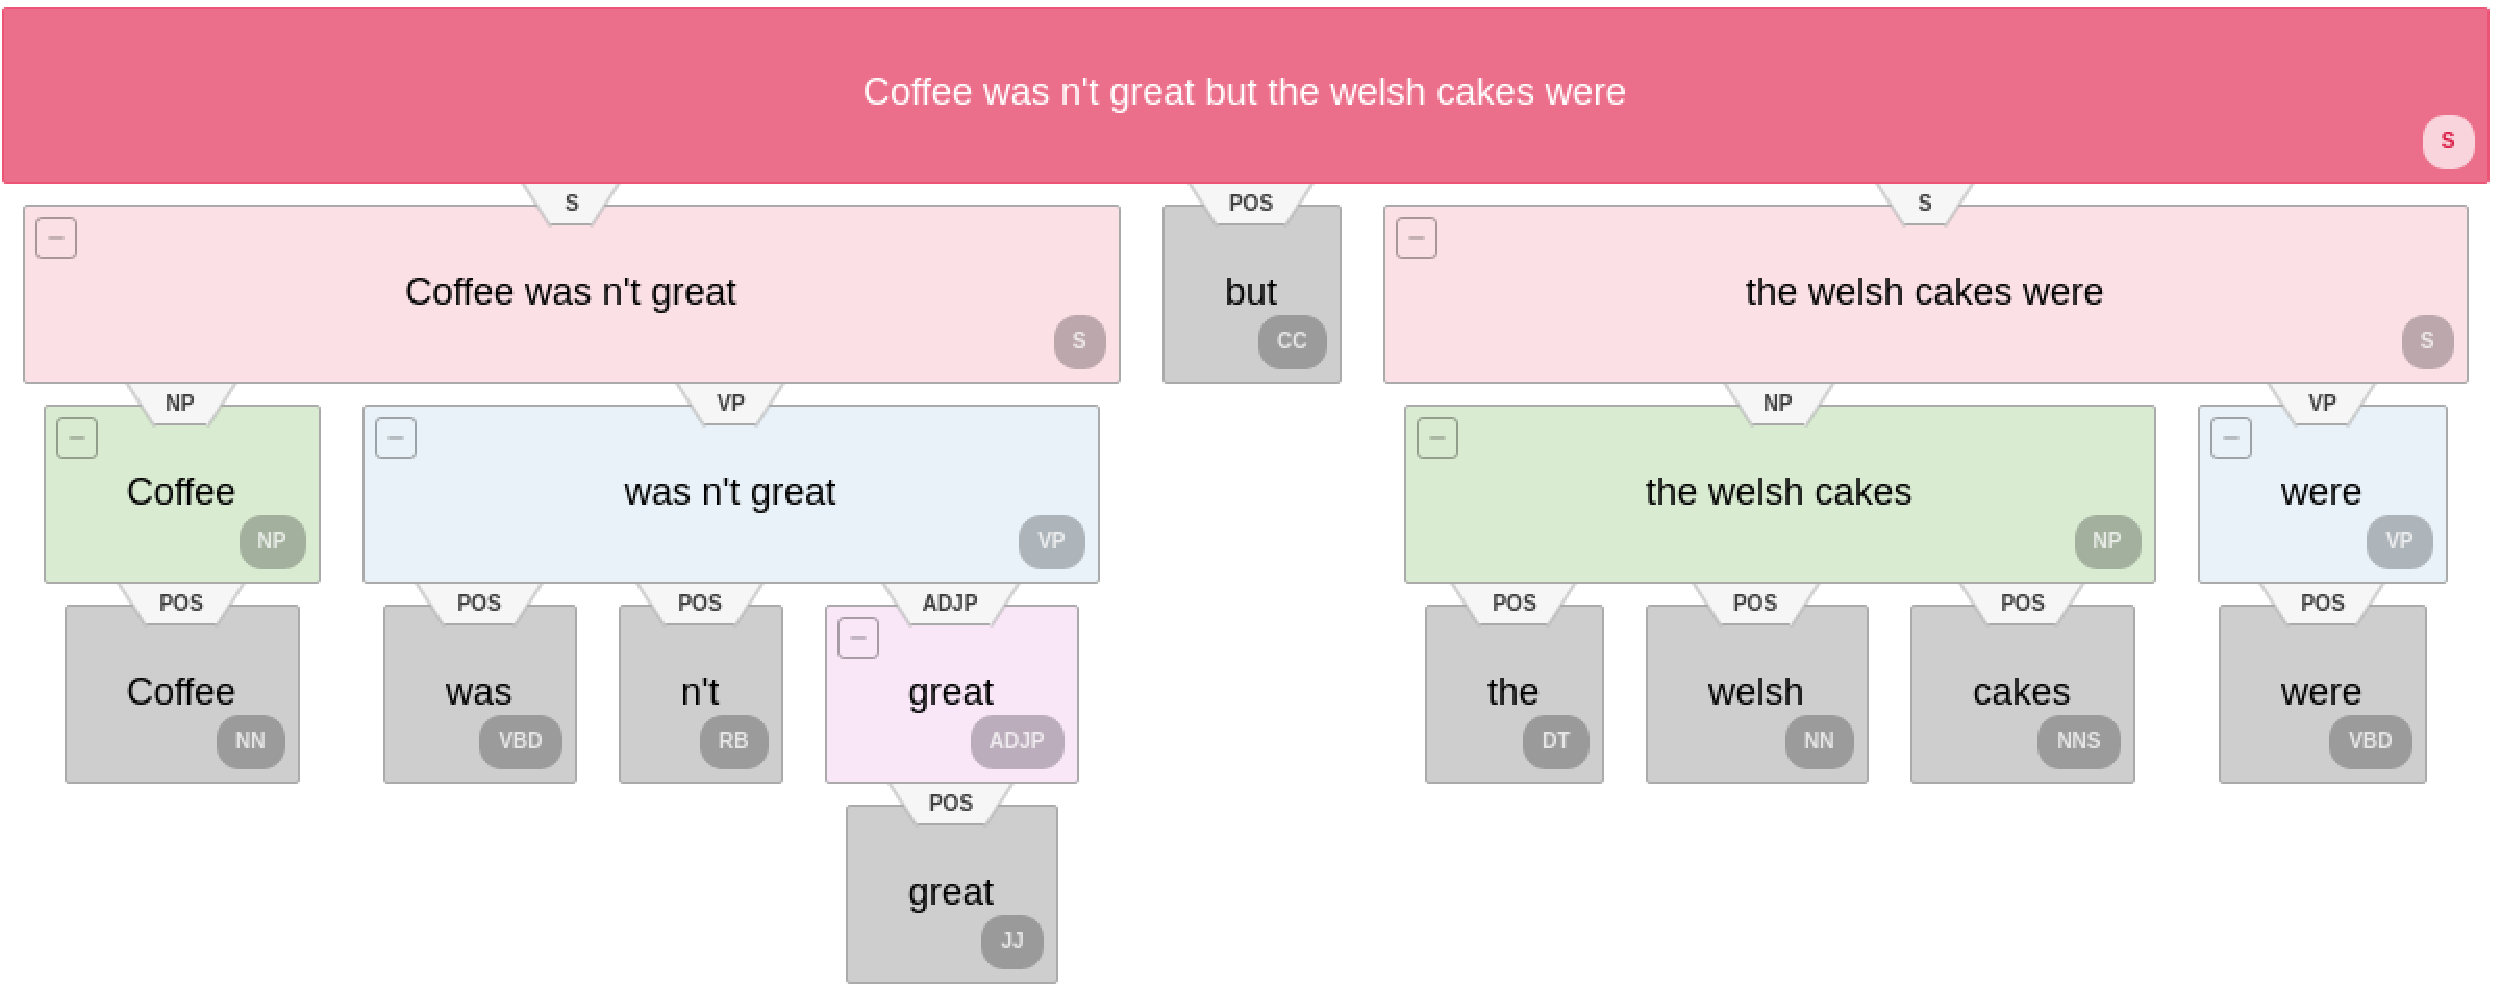
\includegraphics[scale=0.28]{images/lit_review/constituency_tree.pdf}
    \caption{Constituency tree for the sentence `Coffee wasn't great but the welsh cakes were'. The labels in each box represents the constituency label for that span, the labels for the leaf nodes are the POS tags for those words. The tree was created using the AllenNLP demo, which used \citet{joshi-etal-2018-extending} model.}
    \label{fig:lit_review_constituency_tree}
\end{figure}

\begin{figure}[!h]
    \centering
    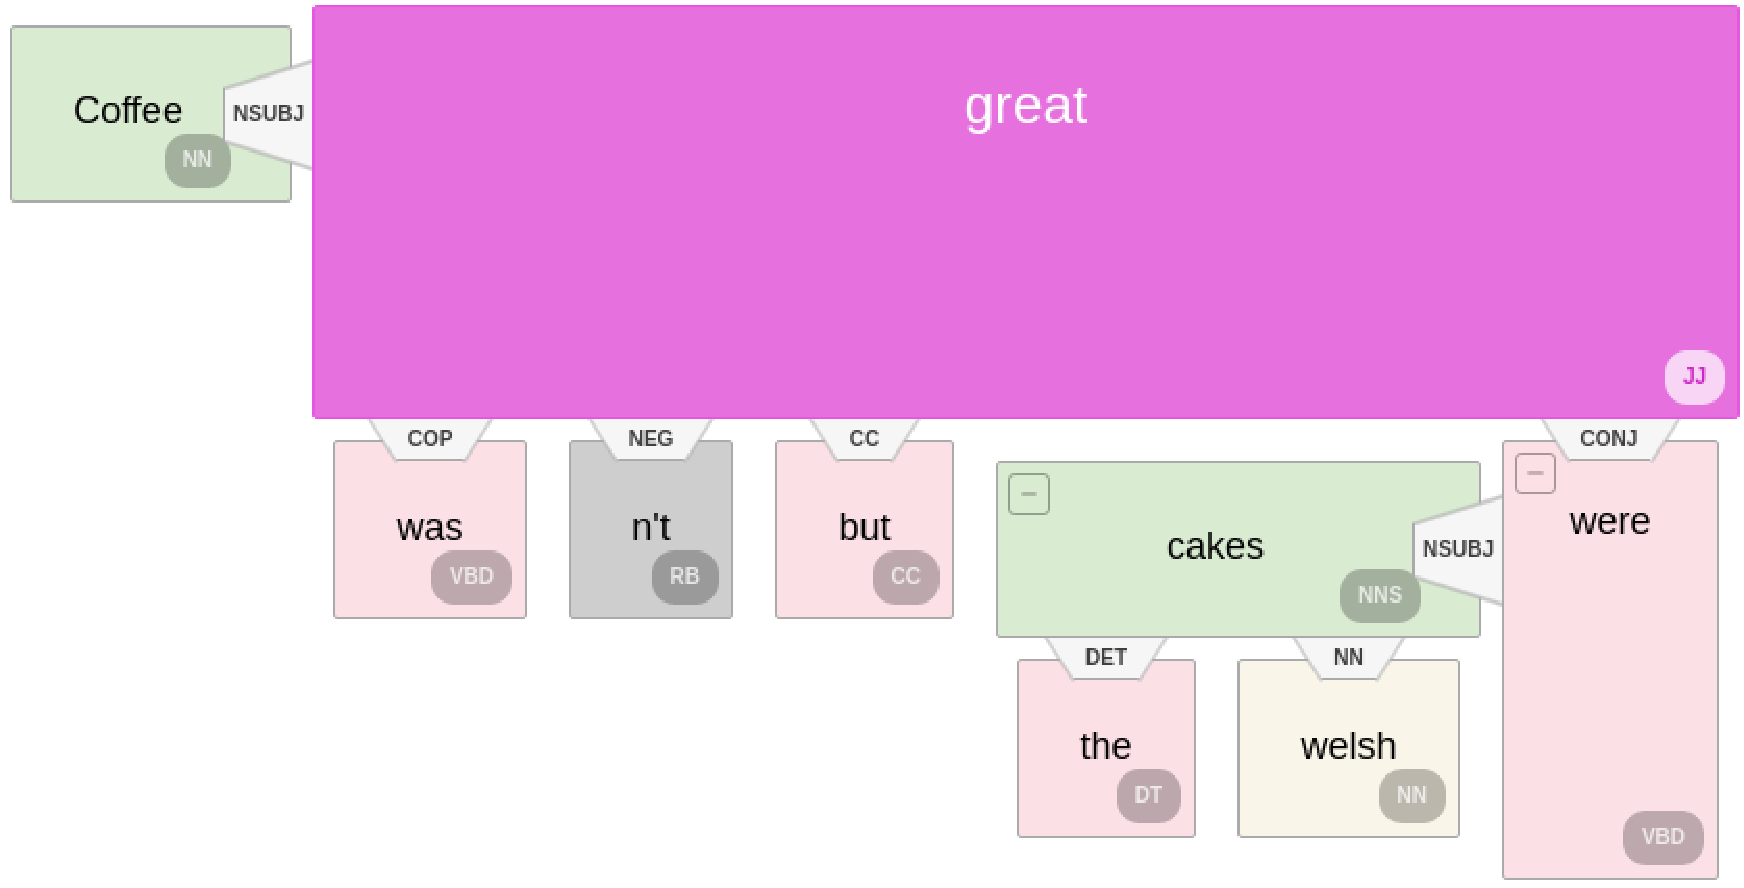
\includegraphics[scale=0.28]{images/lit_review/dependency_parse_tree.pdf}
    \caption{Dependency tree for the sentence `Coffee wasn't great but the welsh cakes were'. The labels within the arcs are dependency labels, and the labels within each box represents the POS tag for the given word. An arc from \textit{word A} to \textit{word B} indicates that \textit{B} is modifying \textit{A}, where \textit{A} is the head word. For example \textit{great} is the head word of \textit{coffee}. The tree was created using the AllenNLP demo, which used \citet{DBLP:conf/iclr/DozatM17} model.}
    \label{fig:lit_review_dependency_parse_tree}
\end{figure}

\section{Sentiment Analysis}
Sentiment analysis can be seen as a more general topic that contains multiple different sub-tasks. These tasks tend to be related and often have different assumptions. In this section, various coarse grained sentiment tasks within sentiment analysis will be discussed starting with the most coarse, document level, and ending with aspect based. During the discussion some important concepts within NLP will also be introduced such as different neural network methods. Throughout the section the different tasks will be shown how they link to each other. The summary of coarse grained sentiment analysis is a primer to the fine grained sentiment analysis review in section \ref{section:lit_review_fine_grained_sentiment_analysis_intro}, which contains the main topic of this thesis Target Dependent Sentiment Analysis (TDSA).

%At the end of the section, the different sentiment tasks will be explicitly shown in terms of how they are related to the main topic of this thesis which is Target Dependent Sentiment Analysis (TDSA).
% Need to mention at the end of this paragraph about poor evaluation and the lack of error analysis showing where alogrthims improve e.g. for generlaising to new targets or targets that exist but with different sentiment. something amybe about generlisation as well.

The many methods that have been used to tackle TDSA and all NLP problems fall into three different categories; supervised, unsupervised, and semi-supervised. Supervised methods require labelled data, in the case of sentiment analysis this would be sentiment labels attached to their relevant text \citep{pang-etal-2002-thumbs}. Unsupervised methods on the other hand only require unlabelled data, which in the sentiment analysis case is just the text. Unsupervised methods within sentiment analysis are normally based around sentiment lexicons (lists\langcorrections{Added s} of words that have an attached sentiment) \citep{hu2004mining} and sometimes a combination\langcorrections{Removed s} of rules \citep{Hutto2014VADERAP}. Thus unsupervised methods tend to require some prior knowledge. Finally,\langcorrections{Added comma} semi-supervised is a combination of the two, learning from both the labelled data and extra unlabelled data \citep{zhu2005semi}. For a more complete overview of the differences between supervised, unsupervised and semi-supervised,\langcorrections{Added comma} see \citet{Weston2007LargeScaleSL}.

\subsection{Document Sentiment Analysis}
The most common sentiment analysis task is that of document level. The task here is given a document which is made up of multiple sentences, to predict the sentiment with the assumption that the document is about one topic \citep{nasukawa2003sentiment}. An example sample for this task can be seen in example \ref{example:lit_review_document_sentiment} where the sentiment of the whole document/review is assumed to be about the movie that is being reviewed. The first to apply a supervised machine learning algorithm to this problem was \citet{pang-etal-2002-thumbs}, where they applied several Machine Learning (ML) classifiers with Bag Of Words (BOW) as features to a new movie review dataset. This line of research of applying ML was further extended by \citet{pang-lee-2004-sentimental} who found that they could reduce the number of sentences by removing objective sentences in the document without significantly impacting, and in some cases improving, the overall accuracy of the classifier. \citet{mullen-collier-2004-sentiment} explored incorporating more semantic features into the BOW models such as the average sentiment values based on the unsupervised techniques of \citet{turney-2002-thumbs}. This approach of adding more semantic information into BOW models was further explored by \citet{whitelaw2005using} who created lexicon feature sets based around appraisal groups. Even though the use of semantic information had improved results \citep{whitelaw2005using}, the strong baseline performance of just using n-gram BOW features was further investigated by \citet{martineau2009delta} who showed that incorporating the class into the TF-IDF weighting mechanism \citep{jones1972statistical} to create Delta TF-IDF significantly improved results. However Delta TF-IDF was only created to work with two classes\footnote{In the sentiment case this is the positive and negative classes.} and not shown to generalise to \textit{n} classes. However a future study by \citet{paltoglou-thelwall-2010-study} showed that further performance gains can be made to TF-IDF based systems by using more enhanced weighting systems like BM25 \citep{robertson1995okapi}.\langcorrections{Indentation added to Example \ref{example:lit_review_document_sentiment}}

\begin{example}
\setlength{\parindent}{17pt}
\indent\textit{a couple of criminals ( mario van peebles and loretta devine ) move into a rich family's house in hopes of conning them out of their jewels . however , someone else steals the jewels before they are able to get to them . writer mario van peebles delivers a clever script with several unexpected plot twists , but director mario van peebles undermines his own high points with haphazard camera work , editing and pacing . it felt as though the film should have been wrapping up at the hour mark , but alas there was still 35 more minutes to go . daniel baldwin ( i can't believe i'm about to type this ) gives the best performance in the film , outshining the other talented members of the cast .}
\caption{Negative document level sentiment example. Document ID \textit{cv435\_24355} taken from \citet{pang-etal-2002-thumbs} sentiment dataset.}
\label{example:lit_review_document_sentiment}
\end{example}

The supervised approaches that have been mentioned so far use a BOW approach, of which this form of vector representation is limited in what it can represent. BOW approaches that use n-gram word features can only learn what a word means within that \textit{n} window. For instance take \textit{n} to be 1 and 2\footnote{i.e. uni-gram and bi-gram features.} it would understand terms such as `very good' and `good' where both would be associated with positive sentiment, however if the statement was `not very good' then it would not capture the full sentiment as it would require all three words to know it is negated. One approach would be to have a very large value for \textit{n}, but this would create a very sparse vector representation which would not generalise well \citep{le2014distributed}. Thus the move away from BOW sparse vector representations to dense word representations was shown to be promising for sentiment analysis in \citet{maas-etal-2011-learning} work. However, this work only found better performance than BOW when they combined the dense vectors with the BOW sparse vector. This first step into dense representation did show some promise as the representation can be learnt from unlabelled data, where they found that results increased when more unlabelled data was used. These dense representations are very similar to what a traditional BOW model learns through its weights within the model \citep{goldberg2017neural}\footnote{See section 2.5.}. The benefit of using the dense representations on the downstream task (sentiment analysis) is that a good representation of the vectors can be learnt from another unsupervised task from unlabelled data first\footnote{The task can also be supervised, but would require labelled data.}. Thus allowing the model to have prior knowledge of what words mean (semantically and syntactically \citep{mikolov2013efficient}) encoded into the vector representation before training the model, unlike the BOW representation which contains no prior knowledge. 

\citet{le2014distributed} showed for the first time how dense vector representations using a NN could surpass BOW representation for which \citet{wang-manning-2012-baselines} set a high baseline at the time for a BOW method. \citet{le2014distributed} created dense document/paragraph vector representations that in comparison to the prior word level versions \citep{maas-etal-2011-learning} could encode document size texts without averaging by learning to predict the next word within a small context window from the document, thus each document vector would be different unlike the word representations\footnote{Unless two or more documents are identical.}. \citet{johnson-zhang-2015-effective} showed that without any additional unlabelled data unlike \citet{le2014distributed} a Convolution NN (CNN) can outperform the BOW approach. The CNN can be seen as a NN approach to a BOW model whereby\langcorrections{Removed space.} the CNN has a set of user defined window sizes of which these window sizes are analogous to n-grams in a BOW model. The CNN differs from the BOW model as it can generalise to unknown n-gram sequences, as it learns how to combine representation from multiple word representations to create the n-gram representation. In comparison for the BOW model it learns what that entire n-gram means and disregards similarities between n-grams based on the words within the n-gram. Furthermore the CNN model does not have the sparsity problem that a BOW model has thus the window size (n-gram in BOW case) can be large;\langcorrections{Added ;} e.g. \citet{johnson-zhang-2015-effective} found that having a window size of 2 and 3 performed\langcorrections{Removed `to` and added `ed` to perform} best\footnote{\citet{le2014distributed} has a good summary of the drawbacks of BOW vector representations.}. For a more complete overview of CNNs, the reader is directed to chapter 13 of \citet{goldberg2017neural}.

None of the above methods, including the NN approach, take into account the word order of the whole document. One family of NN that explicitly encodes the whole sequences\langcorrections{Added `s`} of text in order is the Recurrent NN (RNN) \citep{rumelhart1985learning}. The RNN has several popular variants; Long Short Term Memory (LSTM) \citep{hochreiter1997long} and the Gated Recurrent Unit (GRU) \citep{cho-etal-2014-learning}. \citet{dai2015semi} showed practically that LSTMs can be used for long sequence classification tasks such as document sentiment classification. \citet{xu-etal-2016-cached} created the Cached LSTM to better encode information from large sequences of text, like documents, and showed that it can outperform the LSTM on document sentiment analysis. Hierarchical \citep{zhang2015character} and dilated \citep{strubell-etal-2017-fast} CNN approaches have been created which can capture large contexts,\langcorrections{Added comma} e.g. sentences rather n-grams, where they have been shown to be\langcorrections{added words `to be`} successful in sentiment analysis \citep{conneau-etal-2017-deep}. Finally and more recently, the transformer NN \citep{vaswani2017attention} approach has been applied which does not preserve word order (like the RNN or CNN) but rather treats the text more like a tree structure through attention mechanisms, whereby each word learns to contextualise itself within the text (can be the whole text). The transformer success can be best seen through BERT \citep{devlin-etal-2019-bert} where the architecture can be applied to a task like document sentiment analysis \citep{sun2019fine}\footnote{For a good comparison of RNN, CNN, and transformer based models with respect to computational cost see section 4 of \citet{vaswani2017attention}.}. 

The majority of these more recent NN approaches have been tested on much larger sentiment datasets (100Ks of documents) compared to the earlier work (2-25K documents). It has also been shown that for some of these NN approaches to work well they require extra data \citep{dai2015semi}. However it was found in \citet{dai2015semi} that these NN approaches can make great use of unlabelled data through a language modelling objective. This technique of training on one or more datasets and/or tasks before then applying the model to the end task (in this case document sentiment analysis) is defined as transfer learning in this thesis \citep{ruder2019neural}\footnote{Chapter 3.}.  Both \citet{howard-ruder-2018-universal} and \citet{sun2019fine} found that by pretraining (a type of transfer learning) on the unlabelled data can have large performance gains, making the models more sample efficient with respect to labelled/annotated data. All of the neural methods within this and the last paragraph take into account large contexts of the document,\langcorrections{added comma} if not the whole document, whereas none of the previous methods could effectively do so. This allows the methods to overcome one the main challenges in document sentiment analysis that both \citet{turney-2002-thumbs} and \citet{pang-etal-2002-thumbs} found where the sentiment of the whole document is not the ``sum of the parts'' \citep{turney-2002-thumbs}.

The approaches taken so far treat the document as one large object to encode using some form of supervised method. However there have been methods proposed that suggest it is better to break the document up into smaller linguistic units to encode first into some form of intermediate representation, which is then later combined to generate a sentiment value for the whole document. \citet{bhatia-etal-2015-better} used Rhetorical Structure Theory (RST) \citep{mann-1984-discourse} to create a discourse structure for the document, which\langcorrections{Removed `of` and `this`} can be represented as a dependency-based discourse tree where the nodes are represented by Elementary Discourse Units (EDUs). They found that weighting the outputs of different supervised and unsupervised methods applied to EDUs in the tree based on their depth within the tree improved results. \citet{yang-etal-2016-hierarchical} used sentences to represent the whole document and weighted these sentences and the words within each sentence using two supervised attention mechanisms\langcorrections{Added `s`}. Thus this method unlike \citet{bhatia-etal-2015-better} learnt which sentences and words within those sentences were important to the document's sentiment rather than having a predefined weighting mechanism.

\citet{pang-etal-2002-thumbs} created the first English dataset of movie reviews (1.4K documents), which was later revised and increased in \citet{pang-lee-2004-sentimental} (2K documents), and then increased a lot further by \citet{maas-etal-2011-learning} (25K documents). The prior datasets all contained only two classes, positive and negative, and these were based on the star rating that the movie review was given by the user. \citet{zhang2015character} created four much larger datasets ($600$K -- $4$M\langcorrections{Corrected} documents) that\langcorrections{Removed `have`} originated from Yelp\footnote{https://www.yelp.com/dataset} and Amazon reviews \citep{mcauley2015image} which contain between two and five classes where the classes are based around the user's star rating. This list of English datasets is not supposed to be exhaustive but is given as reference to popular and widely used datasets from the past and current literature.

In this sub-section, document sentiment analysis has been covered with respect to supervised methods and the associated popular English datasets. From the literature it is clear to see that the SOTA are NN based methods that require some form of transfer learning \citep{yang2019xlnet}. All of the methods also clearly point to one of the main challenges in document sentiment analysis which is how best to contextualise the whole document. In the early methods, such as BOW, the methods could only create local contexts through n-grams. This\langcorrections{Added full stop and capitalised `T` on `This`} was\langcorrections{Removed `then`} overcome with NN approaches such as the LSTMs, hierarchical CNNs, and transformers being able to capture the global context of all tokens in the document. Finally within this sub-section different NN approaches have been explained as well as defining the concept of transfer learning.

\subsection{Sentence Sentiment Analysis}
Sentence level sentiment analysis is very similar to document level,\langcorrections{Added level and comma} whereby the only difference is the length of the text to be processed. Due to the length difference, the task is somewhat conceptually easier as a sentence is less likely to have multiple conflicting sentiments, thus the overall sentiment of the sentence is easier to predict. Many different approaches have been used for sentence-based analysis: BOW \citep{wang-manning-2012-baselines}, CNN \citep{kim-2014-convolutional, kalchbrenner-etal-2014-convolutional}, LSTM \citep{brahma2018improved}, and\langcorrections{Added and} BERT \citep{devlin-etal-2019-bert}. However,\langcorrections{Added comma} similar to document level, ``the sentiment of a sentence is not merely the sum of the polarity of the words and phrases found in the text, but rather depends on a number of compositional phenomena that act on\langcorrections{Changed "of" to "on"} indicators of polarity'' \citep{barnes2019improving}. This problem can be best seen in figure \ref{fig:lit_review_sentence_sentiment_example}\footnote{The sentence was chosen from \citet{barnes2019improving} and the figure was generated using the live demo found at this URL \url{http://nlp.stanford.edu:8080/sentiment/rntnDemo.html}.}, where\langcorrections{Removed by from whereby} it can be seen that even though the sentence has multiple positive words the sentiment of the sentence is dominated by the scope of the negation. Due to this, many approaches have been taken to better model the sentiment phrases within the sentence using BOW with compositional semantics \citep{choi-cardie-2008-learning}, Conditional Random Field (CRF) \citep{nakagawa-etal-2010-dependency}, Recursive NN (RCNN) \citep{socher-etal-2012-semantic},\langcorrections{Added comma} deep RCNN \citep{irsoy2014deep}, Tree-LSTM \citep{tai-etal-2015-improved}, Graph NN (GNN) \citep{zhang-zhang-2019-tree}, and multi task learning whereby negation scope and cue detection are the auxiliary task \citep{barnes2019improving}.\langcorrections{In \ref{fig:lit_review_sentence_sentiment_example} complete, removed the `by` after the word `where`.}

\begin{figure}[!h]
    \centering
    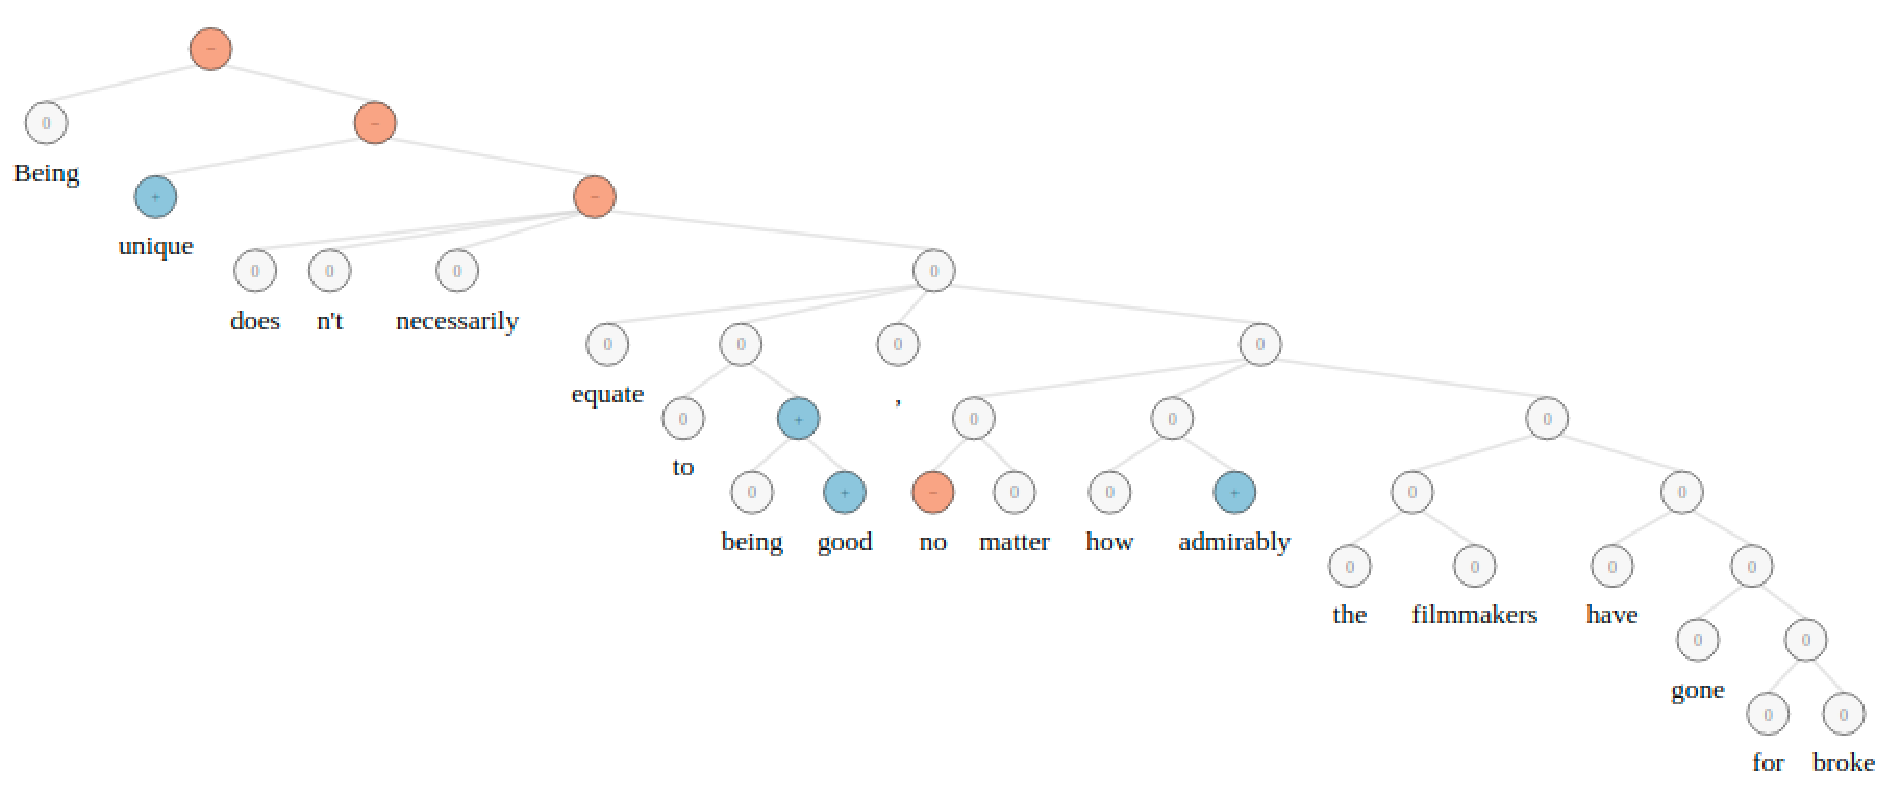
\includegraphics[scale=0.35]{images/lit_review/sentence_sentiment_example.pdf}
    \caption{Phrase and overall sentiment from~\citet{socher-etal-2013-recursive} model, where red, white, and blue represent negative, neutral, and positive sentiment respectively. The sentence in the figure is `Being unique doesn’t necessarily equate to being good, no matter how admirably the filmmakers have gone for broke'.}
    \label{fig:lit_review_sentence_sentiment_example}
\end{figure}

\citet{socher-etal-2013-recursive} took modelling phrases within sentences further by creating a dataset where\langcorrections{Removed "by"} each phrase from the \citet{pang-lee-2005-seeing} movie dataset was manually annotated with a sentiment value, which\langcorrections{Removed "of" and "this"} can be seen in figure \ref{fig:lit_review_sentence_sentiment_example} whereby the model output shown is how the dataset is annotated. Thus this dataset allows models to better capture the compositional phenomena more explicitly by using the phrase level annotation. In a similar trend,\langcorrections{Added comma} \citet{yang-cardie-2014-context} found\langcorrections{Removed "that"} using inter- and intra-sentence\langcorrections{Added hyphens} discourse features to be useful,\langcorrections{Added comma} showing that sentence level classification can be dependent on surrounding sentences. Similarly \citet{mcdonald-etal-2007-structured} found that jointly modelling the sentence and document classification tasks helps improve both. More recently,\langcorrections{Added comma} \citet{angelidis-lapata-2018-multiple} found that by framing document classification as a multiple instance learning (MIL) \citep{dietterich1997solving} problem they were able to create a sentence (EDU) classifier using only the document labels, this outperformed a fully supervised sentence (EDU) level classifier. This MIL method was also shown to be useful when applied to the food health domain \citep{karamanolakis-etal-2019-weakly}.

This review has shown that sentence level sentiment requires both understanding the complex structure within the sentence as well as the more global content of the document. However, even though the literature shows the use of explicitly taking into account phrases and document level information,\langcorrections{Added comma} current SOTA uses the same techniques as that of document level \citep{yang2019xlnet}, utilising transfer learning mainly from a language modelling task. Even so,\langcorrections{Added comma} \citet{barnes-etal-2019-sentiment} have\langcorrections{Changed "has" to "have"} annotated the errors coming from SOTA models into eighteen different categories finding that they perform badly on sentences containing non-standard spellings, idioms, and world knowledge,\langcorrections{Added comma} to name a few. This shows that sentence level sentiment analysis still has plenty of error cases to solve through better incorporating linguistic and world knowledge into new and/or existing methods. To clarify,\langcorrections{Added comma} all of the research mentioned on sentence level sentiment analysis was applied and thus to some extent developed for English. 

\subsection{Aspect Based Sentiment Analysis}
Document and sentence level sentiment analysis both assume that they are discussing one topic \citep{liu2015sentiment}\footnote{Page 47-48.}, for instance if the document (sentence) comes from a review (headline of a review) of the movie, \textit{The Avengers}, the topic that the sentiment is assumed to be about is the movie, \textit{The Avengers}. However, both documents and sentences can contain sentiments on multiple different topics not just the main overall topic of the entire review. Aspect Based Sentiment Analysis (ABSA) attempts to overcome this problem, instead of predicting one sentiment for a document or a sentence it predicts multiple sentiments conditioned on multiple different predefined aspects/topics. ABSA can be performed at different linguistic granularities,\langcorrections{Added comma} typically either document or sentence level. Example \ref{example:lit_review_document_aspect_sentiment} is a Tripadvisor review taken from \citet{Wang2010LatentAR} with seven aspects and their respective sentiments\footnote{They were actually ratings rather than sentiments, but the ratings are used as approximations for sentiment.}, as well as the overall sentiment of the hotel. From this document level ABSA example it can be seen that these aspects are latent, that is the aspect itself does not necessarily occur in the text, this is shown in example \ref{example:lit_review_document_aspect_sentiment} where\langcorrections{Removed "by"} the \textit{service} is negative as the ``Hotel staff speak zero English... The process at the hotel is a bit confusing... staff weren't overly friendly.''. This example would be typically used as a training example for document level ABSA. In this subsection document and sentence level ABSA will be described along with advances in each area and popular datasets.


%Further this example demonstrates that even though the overall sentiment can be negative other aspects can be positive, like the \textit{value} of the hotel. Thus illustrating why document and sentence level sentiment analysis is too coarse and why a more fine grained approach like ABSA is required. 

\begin{example}
\textit{Good and clean but no English spoken The good: The hotel is in a great location and withing walking distance to the Forbidden City and some other sights in this hisrotic district. The rooms were comfortable and clean, really good value.The bad: Hotel staff speak zero English. Breakfast is only Chinese breakfast. The process at the hotel is a bit confusing (make sure you keep those pink receipts they give when you pay, you need them to check out!) and staff weren't overly friendly. Internet is expensive and slow.}
\caption{Example of document level aspect sentiment analysis. The aspects and their receptive sentiments are: \textit{service} (1), \textit{business service} (2), \textit{cleanliness} (3), \textit{check in / front desk} (2), \textit{value} (4), \textit{rooms} (3), and \textit{location} (4). The sentiments were on a scale of 1-5 and the overall sentiment for the review was 2. This was taken from review id \textit{447367} from the trip advisor review dataset of \citet{Wang2010LatentAR}.}
\label{example:lit_review_document_aspect_sentiment}
\end{example}

\subsubsection{Document-level ABSA}
\label{lit_review_document_ABSA}

\citet{snyder-barzilay-2007-multiple} treated the task of document ABSA as a supervised ranking problem, where each aspect is ranked based on a BOW feature vector. They showed the benefit of modelling dependencies between aspects. They found that 38\% of their restaurant review training data contained the same sentiment for all aspects in their respective reviews. Thus they added an agreement function within their model which predicts whether or not all aspects for the review should contain the same sentiment which significantly improved performance. In comparison \citet{Wang2010LatentAR} created the Latent Rating Regression model, which instead of learning from the aspect sentiments can train the model just from the overall sentiment. This therefore reduces the requirement of more fine grained sentiment training data, but the model did require a set of seed words that represented the aspects e.g. for the aspect \textit{room} a set of key words would be \textit{room}, \textit{suite}, \textit{view}, and \textit{bed}. 

More recently, supervised Neural Network (NN) approaches have been the most popular and successful approach to document ABSA. The first to use a NN for document ABSA was~\citet{lei-etal-2016-rationalizing}, whose main aim was to create rationals/explanations for the predictions given only the aspect sentiment labels for supervision.~\citet{yin-etal-2017-document} showed the importance of biasing the attention mechanism within a hierarchical NN~\citep{yang-etal-2016-hierarchical} towards the aspect of interest. The attention mechanism used a set of keywords to define each aspect, from these keywords the attention mechanism would use a memory network~\citep{weston2014memory} to learn how to best describe the aspect so that the model focused on the most important words and sentences in the document.~\citet{yin-etal-2017-document} benchmarked their approach across numerous neural and non-neural approaches.~\citet{li-etal-2018-document} used a similar hierarchical NN as~\citet{yin-etal-2017-document} and found significant performance gains when incorporating both user\footnote{On the dataset that contained user information.} and/or the overall document sentiment information into the attention network. They found that the document sentiment information is useful as the related aspect sentiments are correlated. Further the user information allows the model to better capture textual and sentiment similarities at the aspect level, e.g.,\langcorrections{Added commas} a user tends to have similar sentiment scores for aspects across documents and tends to describe aspects in a similar manner across documents. Finally, the most recent and successful approach used a hierarchical neural Reinforcement Learning (RL)~\citep{williams1992simple} method~\citep{wang-etal-2019-human}\footnote{They called document ABSA, Document-level Aspect Sentiment Classification (DASC).}, whereby\langcorrections{Removed space between "where" and "by"} instead of splitting the document into sentences they used Elementary Discourse Units (EDUs). They used the RL approach to first find aspect relevant EDUs and then within the EDU the relevant aspect sentiment words. They found that if they had used sentences instead of EDUs\footnote{They call EDUs clauses.} then the performance would have decreased by 2.44\% on average, of which they believe this is due to 90\% of EDUs only containing one sentiment~\citep{bayoudhi2015sentiment}. Through error analysis they found that their method performed poorly when negation is used or a comparison is made, however they did not quantify the number of times these errors where made.
% I think we should talk here about sentence level ABSA as the AE literature evaluates some what on both.

% There is also the SemEval review level datasets
There are three main datasets to evaluate document ABSA, Tripadvisor \citep{Wang2010LatentAR}\footnote{This is sometimes called TripDMS.}, BeerAdvocate \citep{mcauley2012learning}, and TripUser \citep{li-etal-2018-document}. Both the Tripadvisor and BeerAdvocate datasets since have been reprocessed by \citet{yin-etal-2017-document} so that aspect sentiments per document are less correlated\footnote{The standard train, development, and test splits for the Tripadvisor and BeerAdvocate datasets can be found here \url{https://github.com/HKUST-KnowComp/DMSC}.}\footnote{The less correlated method comes from \citet[\S5.1]{lei-etal-2016-rationalizing}. They train a linear regression model to predict one of the aspect's sentiment based on all the other aspects sentiments, they then pick the documents that have the largest error until the aspect sentiment correlation in the documents goes beyond a certain threshold.}. This technique of reducing the correlation of the aspect sentiments per document was suggested by \citet{lei-etal-2016-rationalizing}, to ensure that the model does not get ``confused''. It has not been shown whether training models on datasets that have less correlation between aspect sentiments per document produce better models, further \citet{snyder-barzilay-2007-multiple} actually exploited this correlation in their modelling. The Tripadvisor and TripUser are both hotel reviews from the Tripadvisor website\footnote{\url{https://www.tripadvisor.co.uk/}} and contain the same seven aspects, but the TripUser dataset also contains user information unlike Tripadvisor. The BeerAdvocate dataset comes from a beer review website Beeradvocate\footnote{\url{https://www.beeradvocate.com/}} and contains four aspects.

% Need to talk about some point the use of document level as a summary of sentence level which is useful for review websites.
The datasets mentioned so far are all the datasets that have been used\footnote{Or derivatives of.} in the prior work stated in this thesis so far. However these datasets are not expertly annotated data, rather the data has been scraped from their representative websites where the reviews were `annotated' by many different users. One of the few datasets that has been annotated by experts is the SemEval 2016 task 5 subtask 2 dataset~\citep{pontiki-etal-2016-semeval}, which contains seven datasets in five different languages and varies\langcorrections{changed "vary" to "varies"} across three domains\footnote{Restaurant, laptop, and hotel reviews.}. The only methods that have been applied to these datasets are those that entered the SemEval competition.

\subsubsection{Sentence ABSA}
\label{lit_review_sentence_ABSA}

Sentence ABSA unlike document ABSA tends to contain far fewer aspects within its text and unlike document it is rare for a sentence to have all aspects, which is not the case in document ABSA \citep{snyder-barzilay-2007-multiple, Wang2010LatentAR}. All document ABSA methods could be applied to sentence ABSA with minimal changes, however the vast majority of them have been designed for longer texts, for instance the hierarchical NN methods \citep{yin-etal-2017-document, li-etal-2018-document, wang-etal-2019-human}. To further iterate this point on a sentence containing few aspects per sentence,\langcorrections{Added comma} examples \ref{example:lit_review_sentence_aspect_sentiment_1} and \ref{example:lit_review_sentence_aspect_sentiment_2} show two different sentences from the widely used SemEval 2014 task 4 subtask 4 restaurant review dataset \citep{pontiki-etal-2014-semeval}, containing\langcorrections{Removed "each"} one and two aspects respectively. Further,\langcorrections{Added comma} the statistics from the SemEval 2014 restaurant training dataset state that on average each sentence will only have 1.22 aspects\footnote{This was calculated based on the training datasets containing 3041 sentences of which in total there are 3713 aspects within that dataset.} \citep{pontiki-etal-2014-semeval}. In comparison to document, sentence ABSA is less likely to have an \textit{overall} sentiment\footnote{\textit{Overall} sentiment here refers to sentence or document level sentiment, rather than an \textit{overall/general} aspect sentiment e.g. the aspect \textit{RESTAURANT\#GENERAL} in the SemEval 2015 task 12 restaurant dataset \citep{pontiki-etal-2015-semeval}.}, of which some document approaches have made use \langcorrections{removed "of this"}\citep{Wang2010LatentAR, li-etal-2018-document}. Lastly,\langcorrections{Added comma} document ABSA in effect\langcorrections{Changed "affect" to "effect"} summarises the sentiment information for each aspect that has been captured throughout the document, which can make document sentiment analysis a more difficult task if there are lots of contradicting sentiments\langcorrections{Added "s"} for one aspect \citep{pontiki-etal-2016-semeval}.  


\begin{example}
\textit{Overall I would recommend it and go back again.}
\caption{Example of sentence level aspect sentiment analysis. Contains one aspect \textit{anecdotes/miscellaneous} with positive sentiment. This was taken from sentence id \textit{2609} from the trail restaurant dataset of \citet{pontiki-etal-2014-semeval}.}
\label{example:lit_review_sentence_aspect_sentiment_1}
\end{example}

\begin{example}
\textit{Even though its good seafood, the prices are too high.}
\caption{Example of sentence level aspect sentiment analysis. Contains two aspects \textit{food} and \textit{price} with positive and negative sentiment respectively. This was taken from sentence id \textit{3440} from the trail restaurant dataset of \citet{pontiki-etal-2014-semeval}.}
\label{example:lit_review_sentence_aspect_sentiment_2}
\end{example}

Sentence ABSA was popularised by task 4 in SemEval 2014 \citep{pontiki-etal-2014-semeval} where 20 teams created various methods. The winner,\langcorrections{Added comma} \citet{kiritchenko-etal-2014-nrc},\langcorrections{Added comma} used a Support Vector Machine (SVM) \citep{chang2011libsvm} with different BOW features including ngrams, POS tags, and various in and out of domain sentiment lexicon features\footnote{Sentiment lexicon is a collection of different groups of words where each group is associated to a specific sentiment. This definition follows that of \citet{mohammad-turney-2010-emotions} for their emotion lexicon definition if you substitute emotion for sentiment.}. To\langcorrections{Removed "Further"} better capture the aspect specific sentiment,\langcorrections{Added comma} they utilised a domain adaptation technique \citep{daume-iii-2007-frustratingly} such that each aspect category had its own BOW weight vector that was learnt at the same time as the general BOW weight vector, so that aspect specific and general features can be learnt separately. SemEval repeated a similar task for two more years, 2015 and 2016, where\langcorrections{replaced "when" with "where"} the winners all use a similar BOW approach \citep{saias-2015-sentiue, brun-etal-2016-xrce, kumar-etal-2016-iit}. 

NN approaches for this task are desirable due to them requiring fewer linguistic resources, and the ease of transferring the approach to multiple languages \citep{ruder-etal-2016-insight-1}. \citet{ruder-etal-2016-insight-1} applied a CNN to the task outperforming many of the aforementioned BOW approaches on multiple languages. In later work \citet{ruder-etal-2016-hierarchical} showed that taking into account the surrounding sentences using an hierarchical LSTM further improved results. \citet{wang-etal-2016-attention} found that by adding attention to a sentence level LSTM improved the model by allowing it to better capture relevant aspect specific words within the sentence. Follow on work \citep{bao-etal-2019-attention} found that regularising the attention network using sentiment lexicons and/or attention sparsity improved the robustness of the model. \citet{wang2018aspect} utilised a hierarchical NN similar to \citet{yin-etal-2017-document} (document ABSA) whereby the hierarchy of the sentence was based around EDUs within the sentence, and the words within those EDUs. This was proposed on the premise that EDUs often discuss one aspect, thus making the task for the NN easier, as the model could ignore EDUs that were not discussing the relevant aspect. They found this hierarchical approach to outperform the flattened version. Current SOTA approaches utilise transfer learning from Bi-directional Language Models (BiLM) \citep{sun-etal-2019-utilizing, jiang-etal-2019-challenge} (also known as Contextualised Word Representations (CWR) which is what they will be called from now on).\langcorrections{Explained CWR}

Compared to the previous approaches \citet{kaljahi-foster-2018-sentiment} explored whether adding the aspect's sentiment expressions to a model would improve results. The sentiment expression which is ``part of the sentence which conveys the sentiment towards a certain aspect'' \citep{kaljahi-foster-2018-sentiment} was added to the English SemEval 2016 laptop and restaurant datasets. Example \ref{example:lit_review_sentence_aspect_sentiment_expression} demonstrates what an aspect's\langcorrections{added apostrophe} sentiment expression is. They found that\langcorrections{Replaced "by" with "that"} adding the sentiment expressions into the NN model improved results greatly, however in this setup at test/inference time the model would require the aspect's\langcorrections{Added apostrophe} sentiment expression. To overcome this they incorporated the sentiment expressions in a multi task setup, but this led to the model performing as well as a model that did not require sentiment expressions. This line of research shows promise as it demonstrates that using aspect sentiment expressions can improve results but incorporating this information into a model that does not require it at test time is difficult. Further aspect sentiment expressions, if they could be predicted at the same time as the sentiment, could create some form of explanation to the sentiment prediction, making the black box NN methods more explainable,\langcorrections{Added comma} which is similar to what \citet{lei-etal-2016-rationalizing} did in document ABSA.

\begin{example}
\textit{However, go for the ambience, and \textbf{consider the food just a companion} for a trip across the world!}
\caption{Aspect sentiment expression example, where the sentiment expression is in \textbf{bold} for the related aspect \textbf{food\#quality}. This was taken from the SemEval 2016 Restaurant dataset \citep{pontiki-etal-2016-semeval} with the additional sentiment expression labelled by \citet{kaljahi-foster-2018-sentiment}.}
\label{example:lit_review_sentence_aspect_sentiment_expression}
\end{example}

% Need to mention at some point the link between the 2016 sentence and document ABSA this is not the same as target also linked through the sentence and i assume review id.
Popular sentence ABSA datasets for English are the SemEval 2014\footnote{The restaurant ABSA dataset partially came from \citet{Ganu2009BeyondTS}.} \citep{pontiki-etal-2014-semeval}, 2015 \citep{pontiki-etal-2015-semeval}, and 2016 \citep{pontiki-etal-2016-semeval} datasets for the laptop, restaurant, and\langcorrections{Added "and"} hotel review domain\footnote{The 2014 datasets ABSA annotation was only provided for the restaurant domain.}. A large difference between the 2015 and 2016 datasets compared to the 2014 was the sentiment of an aspect may require a larger context than just the sentence the aspect appeared in, hence why the whole review was given as context. The 2016 SemEval dataset also expanded the number of languages from just English to six more languages\footnote{The six languages are; Dutch, French, Russian, Spanish, Arabic, and Chinese.}. Also,\langcorrections{Added comma} as stated in the last paragraph, \citet{kaljahi-foster-2018-sentiment} annotated the English SemEval 2016 laptop and restaurant dataset with sentiment expressions. There has also been a challenge dataset, Multi-Aspect Multi-Sentiment (MAMS) \citep{jiang-etal-2019-challenge}, which is within the restaurant review domain\footnote{This dataset was created from the same source of restaurant reviews as the SemEval 2014, 2015, and 2016 restaurant dataset, which was the Citysearch New York dataset by \citet{Ganu2009BeyondTS}.}, unlike the other datasets it ensures that each sentence contains at least two aspects and at least two different sentiments per sentence.

Sentence level ABSA has also been known as topic sentiment analysis within the Twitter sentiment analysis community. Topic sentiment analysis has been run as a competition three times at SemEval \citep{rosenthal-etal-2015-semeval, nakov-etal-2016-semeval, rosenthal-etal-2017-semeval}, each year creating a new larger dataset for English and in the final year (2017) creating an Arabic Twitter dataset as well. In their first year of running the competition (2015) they also ran a task (D) which they described as ``sentiment towards a topic in a set of tweets'' which can be viewed as a document ABSA task. These datasets are also annotated for Tweet/sentence sentiment as well as the topic, the 2017 dataset contains user information, and the 2015 dataset is also annotated with sentiment expressions.

From this section on ABSA prior work it is clear that there is plenty of future work that can be explored. Creating more robust models is important,\langcorrections{Added comma} especially for real world applications.\langcorrections{Added "s" and removed "of which"} \citet{bao-etal-2019-attention} explored this problem, however they only evaluated on one dataset, thus expanding this evaluation for more datasets and across a spectrum of low to high resource settings would be of use to better understand how robust their method is. An unexplored area is the link between sentence and document ABSA whereby one would assume that document ABSA should improve the performance of sentence and vice versa, of which this can be empirically tested using the SemEval 2015 \citep{pontiki-etal-2015-semeval} and 2016 \citep{pontiki-etal-2016-semeval} review datasets.



% For a good overview of cross-lingual approaches to sentiment analysis at both the sentence and target level see \citet{barnes2019cross} thesis.

%\citet{marcheggiani2014hierarchical} used a CRF model with various BOW features for aspect identification and sentiment prediction, where by they found jointly modelling the aspect and overall review sentiment to be beneficial for aspect sentiment prediction but not identification. Further they also introduced a sentence level English ABSA dataset with review/document level annotation for the hotel domain. 
%Adding user information into sentiment analysis methods has been done

%In a similar line of work Aspect Extraction (AE) is the task of predicting the aspects that the text is discussing, again AE can also be performed typically at document or sentence level. In example \ref{example:lit_review_document_aspect_sentiment} the review has a set of predefined aspects, but not all reviews will always have all of these predefined aspect some may have fewer aspects, and in other domain like Laptop reviews may contain more aspects. For document AE \citet{titov2008modeling} created Multi-grain LDA (MG-LDA) a modified version of Latent Dirichlet Allocation (LDA) for the task of unsupervised document AE. MG-LDA compared to LDA creates two groups local and global where by they found that a local groups better correspond to aspects. To empirically validate their method they showed that adding the MG-LDA features to the \citet{snyder-barzilay-2007-multiple} model improved results and also out performed using the LDA features instead. The drawback of topic modelling methods like LDA or MG-LDA is the requirement of setting the number of topics that the model is required to generate, and then having to manually label which topics correspond to which aspects, if the topics do correspond to any of the predefined aspects. In comparison to this completely unsupervised approach \citet{mukherjee-liu-2012-aspect} used a set of seed words and known number of aspects/topics to constrain their topic modelling based method, which is similar to \citet{Wang2010LatentAR}. 

% A problem with all of these topic modelling based approaches is that it cannot assign a document/text to an aspect or a number of aspects without, the most interesting part of these type of clustering is that it can define what words are in what aspect clusters.
% The existing models that do use seeds can also generate more topics that have not been seeded and they judge if the topic is relevant by looking at the terms in the topic and judging using human knowledge.

%More recent approaches have moved away from topic modelling like LDA to Neural Networks (NN). \citet{he-etal-2017-unsupervised} used an autoencoder styled unsupervised learning objective where by the NN was trained to reconstruct the encoded sentence from a dense matrix that would represent aspects. From this aspect matrix they could find words associated to an aspect using a similarity function between the aspect matrix and a word's vector representation/embedding. Further they could also assign a text to a single aspect label\footnote{The method could not assign more than one label to a text. This could be done but would require some form of threshold/confidence level on the output of the softmax in equation 6.} based on the output of the NN. This approach was later improved upon by \citet{angelidis-lapata-2018-summarizing} where the aspect matrix was initialised using a weighting approach from the embeddings of known aspect seed words, these seed words and their weighting did come from a limited amount of labelled data. Further they showed the benefit of using a multi task learning objective where by predicting the domain of the sentence\footnote{In this work instead of sentences they used EDUs.} was beneficial, as they believed domain relevant words were also relevant to the aspect. 

%\citet{karamanolakis-etal-2019-leveraging} showed how to better utilise known aspect seed words through a student-teacher distillation model \citep{bucilua2006model, hinton2015distilling}, where by the teacher predicted the probability of each aspect for a sentence based on the frequency of the aspect seed words in the sentence\footnote{A special version of a BOW model.}. The student model then learnt off the teacher's model predictions thus not requiring any human annotated data. The teacher's model was then updated using the student predictions on the training data in a co-training setup \citep{blum1998combining}. Thus allowing the teacher to learn weights for each of the seed words, this improved teacher model then re-taught the student model, of which this process is then repeated until the predictions from the teacher and student are similar. The student model is then used to predict which aspect occurs in the text. The advantage of this student model approach unlike the previous NN approaches \citep{he-etal-2017-unsupervised, angelidis-lapata-2018-summarizing} it allows the student model to be any type of model. However they found that averaging word vectors similar to \citet{he-etal-2017-unsupervised, angelidis-lapata-2018-summarizing} to perform well and outperforms all existing unsupervised approaches\footnote{Approaches that use seed words tend to be called weakly supervised rather than unsupervised. This is due to the approach requiring some knowledge that has had to come from a human annotator. However in this part of the literature review we have grouped the unsupervised and weakly supervised together and have explicitly stated at each point if the method required seed words.}.
% next prehaps talk about different ways these are evaluated, may need to introduce the sentence level stuff.

%In all of the previous work ABSA and AE has been discussed at the document level. However there are some noticeable problems with performing at this granularity. For AE, if the set of predefined aspects is known, like the seven aspects in example \ref{example:lit_review_document_aspect_sentiment}, then in most cases due to the size of the documents most of the aspects will be within the document thus making the task 

%To overcome the problem that aspects can have multiple sentiments throughout a document or a sentence \citet{lazaridou-etal-2013-bayesian} setup the AE and ABSA task at the Elementary Discourse Unit (EDU). They also performed their analysis at this linguistic unit as they hypothesised that either the aspect and/or sentiment that the unit will be discussing will change at the start of an EDU. They found that incorporating knowledge of this aspect/sentiment change into their weakly supervised LDA model for AE and ABSA improved results. However performing AE and/or ABSA at EDU level never progressed any further than this line of work.

%A sample of sentence and Tweet can be seen in example. The reason for grouping both sentence and Twitter based methods is due to the fact that Tweet based methods can be seen as a adaptation of sentence based method to a different type of text. 


%The main difficulty in document sentiment analysis has been shown through it's length Further sentiment lexicons have been defined and numerous NN methods have been introduced. 

%So far the supervised methods within document sentiment analysis have been covered, from which it is clear to see that the SOTA are NN based and require some form of transfer learning \citep{yang2019xlnet}. All of the methods also clearly point to one of the main challenges in document sentiment analysis is the size of the documents. This can be seen from early in the literature where  \citet{turney-2002-thumbs} state that the sentiment of the whole document is not the `sum of the parts'. This therefore means that the whole document needs to be understood in context to fully understand the sentiment which has been shown not possible with the BOW methods. Thus the move to NN approaches such as the LSTMs, heirahcical CNNs, and transformers to overcome this problem.


%can be used to c encode some form of word order within 
%The use of dense vector representations stayed at the forefront to State Of The Art (SOTA) document sentiment classification. 

% created a much large movie review sentiment dataset \citet{maas-etal-2011-learning}
%who explored different information retrieval weighting mechanisms

%\citet{whitelaw2005using} Created a apprisal lexicon through using a list of words that were known to be part of the lexicon as `seed words' and then expanding that list through collocations, WordNet, and thesauri

%Incorporating 

%The first document sentiment dataset was by \citet{pang-etal-2002-thumbs}, which was then later enlarged by \citet{pang-lee-2004-sentimental}

%This novel Machine Learning (ML) work was conducted at the same time as \citet{turney-2002-thumbs} who applied an un-supervised approach to the same problem, both came across the same problem, which is that the sentiment of the review cannot be determined through `sum of it's parts' \citep{turney-2002-thumbs}\footnote{This is paraphrased for grammatical reasons, the actual quote is `sum of the parts'}. This problem is due to both works only using BOW (up to bi-grams) features within their methods, thus their features only take into account local context and limited linguistic knowledge (POS tags in \citet{turney-2002-thumbs}). This problem to some extent started to be alievated with the raise of more 

\section{Fine Grained Sentiment Analysis}
\label{section:lit_review_fine_grained_sentiment_analysis_intro}

Compared to the previous sections, this as the name suggests, is the most detailed granularity of sentiment analysis. Fine grained sentiment analysis is made up of many different tasks where the results of these tasks when combined creates the information required to fully understand a sentiment in context. The literature has been very clear on the following tasks being at the core of understanding sentiment in context \citep{wiebe-1994-tracking, kim-hovy-2004-determining, ding2008holistic, liu2015sentiment}:
\begin{enumerate}
    \item Identifying the holder of the sentiment.
    \item Identifying the target/object of the sentiment within the text\footnote{In \citet{ding2008holistic} they use the word feature to mean target. In \citet{kim-hovy-2004-determining} they use topic to mean target.}.
    \item The sentiment of the holder towards the target.
\end{enumerate}

The information from these three tasks creates a triplet of information (sentiment holder, target, sentiment) to define the whole fine grained sentiment task. To better understand this,\langcorrections{Added comma} example \ref{example:lit_review_fine_grained_sentiment_analysis_1}\footnote{In all examples the target will be in bold, the sentiment words within the text in the colour of their sentiment, and the holder underlined. The sentiment colours are \negbox{pink for negative}, \neubox{grey for neutral}, and \posbox{blue for positive}.} contains five triplets; (author, food, negative), (Jonathan, bara brith, positive), (He, leeks, neutral), (June, Welsh fruit cake, negative), and (June, chocolate cake, positive). 


\begin{example}
\textit{(1) The \textbf{food} at the store was \negbox{horrible}, but \underline{Jonathan} thought the \textbf{bara brith} was \posbox{fantastic}.(2) \underline{He} did think the \textbf{leeks} were \neubox{so so}. However \underline{June} found the \textbf{Welsh fruit cake} to be \negbox{tasteless} but the \textbf{chocolate cake} to be \posbox{great}.}
\caption{Made up fine grained sentiment analysis example written on the 24\textsuperscript{th} May. For reference bara brith is a kind of fruit cake that was created in Wales.}
\label{example:lit_review_fine_grained_sentiment_analysis_1}
\end{example}

The triplet of information, which to some degree, was first defined within \citet{wiebe-1994-tracking} when stating the components of a private state\footnote{Page number 235 of \citet{wiebe-1994-tracking}, defines experiencer, attitude, and object as the components of a private state. Experiencer, attitude, and object can be mapped to holder, target, and sentiment within the triplet of information definition.} has been expanded by \citet{liu2015sentiment} who has created the clearest and most detailed definition so far and builds upon the previous work \citep{wiebe-1994-tracking, kim-hovy-2004-determining, ding2008holistic}. Liu's \citep{liu2015sentiment}\langcorrections{Added apostrophe} basic quadruple definition\footnote{Definition 2.1 in \citet{liu2015sentiment}.} is the same as the triplet so far with the added information of time. The importance of time within the definition is argued as sentiment can change over time, which is of importance for real world applications as one may want to know how a holder's\footnote{A more concrete example of a holder could be a politician, whereby the application may want to see when/if they changed their sentiment towards a bill/law.} sentiment changes. 

This quadruple definition is then expanded to a more detailed quintuple definition\footnote{Definition 2.7 \citet{liu2015sentiment}.}, with the target of the sentiment replaced with entity and aspect of the sentiment; (sentiment holder, aspect, entity, sentiment, time). Both the entity and aspect are latent in that they do not have to link to any part of the text unlike the target within the triplet. Further, the aspect and entity are linked via a hierarchical structure as in the aspect would be either an attribute or part-of the entity. The motivation behind removing the target and replacing it with the aspect-entity pairing is so that targets can be better grouped together. For instance, in example \ref{example:lit_review_fine_grained_sentiment_analysis_1} even though both June and Jonathan are discussing the same food produce (bara brith) due to the different ways of stating it, grouping would have to occur to know they are discussing the same thing. The benefit of this aspect grouping is that from an application perspective an end user can get an overall trend of a sentiment towards aspects\langcorrections{Added "s"} and entities of interest rather than sentiment towards targets, given that there could be exponentially more targets compared to aspect-entity pairs. To make the quintuple definition more concrete, the quintuples for example \ref{example:lit_review_fine_grained_sentiment_analysis_1} are; (author, GENERAL, FOOD, negative, 24\textsuperscript{th} May), (Jonathan, CAKE, FOOD, positive, 24\textsuperscript{th} May), (He, VEGETABLES, FOOD, neutral, 24\textsuperscript{th} May), (June, CAKE, FOOD, negative, 24\textsuperscript{th} May), and (June, CAKE, FOOD, positive, 24\textsuperscript{th} May).

The problem with the quintuple definition is that it is lacking in target information. Even though the target might be too fine grained for some applications, it can be useful for training models as the position of the target is useful for inferring the sentiment \citep{gu-etal-2018-position}. More so there could be a case where a text contains two contradicting sentiments for the same aspect-entity pair, holder, and time. This can be seen in example \ref{example:lit_review_fine_grained_sentiment_analysis_1}\langcorrections{Added example reference} whereby June is negative about the Welsh fruit cake but positive about the chocolate cake. This would be confusing for training a machine learning model as the same text contains contradicting sentiments for the same aspect, entity, holder, and time. This problem of having two contradicting sentiments for the same information and text is defined in this thesis as sentiment ambiguity, in this case the information is aspect-entity pair, holder, and time. To avoid this sentiment ambiguity problem one could simply create more detailed aspect or entities which to some degree is suggested in \citet{liu2015sentiment}\footnote{On page 22-23 of \citet{liu2015sentiment} they state that if the user wants more detailed information then more entities would need to be created, and they use a printer and its ink as an example.} or as proposed in this thesis, add the target to the quintuple to create the hextuple as in\langcorrections{Added "as in"} definition \ref{definition:lit_review_fine_grained_sentiment_analysis_hextuple}. To make this concrete, the following are hextuples for example \ref{example:lit_review_fine_grained_sentiment_analysis_1}; (author, food, GENERAL, FOOD, negative, 24\textsuperscript{th} May), (Jonathan, bara brith, CAKE, FOOD, positive, no time given), (He, leeks, VEGETABLES, FOOD, neutral, 24\textsuperscript{th} May), (June, Welsh fruit cake, CAKE, FOOD, negative, 24\textsuperscript{th} May), and (June, chocolate cake, CAKE, FOOD, positive, 24\textsuperscript{th} May). It is clear that these hextuples remove any remaining sentiment ambiguity in comparison to their quintuple counterparts from the previous paragraph. Note,\langcorrections{Added comma} in general not all of the values of these hextuples must be filled but rather the more that are filled potentially less ambiguous the sentiment would be and more detailed analysis can be performed,\langcorrections{Added comma} e.g. sentiment over time or comparing sentiment of different holders on a particular target/aspect/entity.

\begin{definition}
Hextuple fine grained sentiment definition: (h, t, a, e, s, ti). Where h = sentiment holder, t = target, a = aspect, e = entity, s = sentiment, and ti = time.
\label{definition:lit_review_fine_grained_sentiment_analysis_hextuple}
\end{definition}

Lastly, we state here some explanations and edge cases that come from the hextuple definition. The sentiment holder can be very important in sentiment disambiguation as shown by example \ref{example:lit_review_fine_grained_sentiment_analysis_2} sentence 2, which without the sentiment holder information it would be unclear what the sentiment value is for `talks', as Lucy found it negative and Joe positive. However, \citet{liu2015sentiment} motivated the reason for the sentiment holder\footnote{This was on page 18 of \citet{liu2015sentiment}.} within the sentiment definition is\langcorrections{Author added "is"} due to the potential influence difference between different holders,\langcorrections{Added comma} e.g. an online influencer sentiment towards a target/product could be more important than an\langcorrections{Author changed "a" to "an"} everyday customer. Within this thesis the importance of influence of the holder is recognised for applications.\langcorrections{Removed "but" and created new sentence} From a sentiment perspective example \ref{example:lit_review_fine_grained_sentiment_analysis_2} sentence 2 shows the main reason for the holder being required in the sentiment definition, to resolve sentiment ambiguity. Additionally,\langcorrections{Added comma} the target within the hextuple can be empty due to the target being,\langcorrections{Added comma} implicit thus this is when the aspect-entity pair is required to resolve what the implicit target is, this is shown on sentence 3 in example \ref{example:lit_review_fine_grained_sentiment_analysis_2}. Also,\langcorrections{Added comma} the aspect within the aspect-entity pair is not always required if a hierarchical structure is not required as only the entity is needed to resolve implicit target situations, as shown in sentence 3 of example \ref{example:lit_review_fine_grained_sentiment_analysis_2}. Finally,\langcorrections{Added comma} as shown in example \ref{example:lit_review_fine_grained_sentiment_analysis_2} sentence 1,\langcorrections{Added comma} the time element could be required to disambiguate the sentiment, however the time effect is a very small edge case. This concludes the motivation and reason behind the new fine grained sentiment definition of the hextuple, which can be seen as a direct extension and backward compatible with the previous definitions.

\begin{example}
\textit{(1) \underline{Ben} used to \posbox{love} \textbf{lectures} but no longer due to the new lecturer. (2) \underline{Lucy} did \negbox{not \posbox{enjoy}} the \textbf{talks} but \underline{Joe} did. (3) \underline{Dave} \posbox{loved} \textbf{University} but found it \negbox{expensive}.}
\caption{Made up fine grained sentiment example. This example contains the following hextuples; (Ben, lectures, LECTURES, EDUCATION, positive, past), (Ben, lectures, LECTURES, EDUCATION, negative, present day), (Lucy, talks, LECTURES, EDUCATION, negative, past), (Joe, talks, LECTURES, EDUCATION, positive, past), (Dave, university, -, EDUCATION, positive, present), and (Dave, -, PRICE, UNIVERSITY, negative, present). The dash (-) symbol within the hextuple represents the value not existing.}
\label{example:lit_review_fine_grained_sentiment_analysis_2}
\end{example}

% This needs changing.
Datasets that could\langcorrections{Added "could" and removed some words from the start of the sentence.} make\langcorrections{Removed "s"} use of part of these hextuples are the popular SemEval 2015 and 2016 restaurant datasets,\langcorrections{Added comma} which contain\langcorrections{Removed "s"} (target, aspect, entity, sentiment) values of the hextuple. This\langcorrections{Removed "Furthermore"} thesis has found that without including the target within the hextuple it would be impossible to classify\langcorrections{Removed "all"} 3.68\% and 3.27\% of samples correctly from the 2015 and 2016 datasets respectively due to sentiment ambiguity\footnote{URL to the python notebook that reproduces this result \url{https://bit.ly/3gtx1RN}.}. This is due to texts containing the same aspect-entity pair more than once with different sentiments. Even though these percentages are small it further empirically justifies why it is needed to include the target within the hextuple definition.

\citet{wiebe-1994-tracking}\langcorrections{Removed some words from the start of the sentence} described that the private state, which can be seen as the original fine grained sentiment definition, can only be found in subjective sentences. Thus the fine grained sentiment cannot be used within objective sentences or in objective cases. In this thesis it is argued that objective sentences can contain fine grained sentiment as stated in section 2.4.2 of \citet{liu2015sentiment}. Example \ref{example:lit_review_fine_grained_sentiment_analysis_3}\langcorrections{Changed example \ref{example:lit_review_fine_grained_sentiment_analysis_3} from positive to negative} shows an objective negative sentiment towards Rio tinto, this is also an example of implicit sentiment which is discussed in more detail in subsection \ref{lit_review_further_related_topics_implicit_and_factual_Sentiment}.

\begin{example}
\textit{(1) \textbf{Rio tinto} shares went down on the 22\textsuperscript{nd} of May.}
\caption{Made up fine grained objective sentiment example. This example contains the hextuple (Author, Rio tinto, MINING, STOCKS, negative, 22\textsuperscript{nd} of May).}
\label{example:lit_review_fine_grained_sentiment_analysis_3}
\end{example}

Given this hextuple definition \ref{definition:lit_review_fine_grained_sentiment_analysis_hextuple} it is clear how sentence and document ABSA from the last two subsections \ref{lit_review_sentence_ABSA} and \ref{lit_review_document_ABSA} can be ambiguous with respect to sentiment. This is best shown in example \ref{example:lit_review_fine_grained_sentiment_analysis_2} whereby in sentence 1 for the aspect-entity pair (LECTURES, EDUCATION) there is both a positive and negative sentiment, thus from a ABSA perspective it would be impossible to capture both sentiments. This case will become more problematic with longer texts e.g. document ABSA, as they are more likely to contain multiple of the same aspect with different sentiment. Hence as stated in the opening paragraph of sentence ABSA subsection \ref{lit_review_sentence_ABSA}, document ABSA in effect summarises the sentiment information of aspects, and this would have to happen when ambiguities occur at the sentence level as well as is the case within example \ref{example:lit_review_fine_grained_sentiment_analysis_2} sentence 1. To make this more concrete, the aspect summary for the aspect-entity pair (LECTURES, EDUCATION) in sentence 1 of  example \ref{example:lit_review_fine_grained_sentiment_analysis_2} could be neutral as there\langcorrections{Changed "their" to "there"} is both a positive and negative sentiment towards the aspect-entity pair.

The main tasks to create the hextuple are the following:
\begin{description}
    \item[Task 1] Target extraction.
    \item[Task 2] Entity and Aspect mapping. Due to the cases of implicit targets, one would have to treat this task as ABSA extraction\footnote{This task is described as aspect category detection in \citet{pontiki-etal-2016-semeval}.} for the given text, as one cannot assume that a target is always in the text. Then given the aspect-entities that have been extracted for the text map them to the targets extracted as well as a special implicit target symbol if implicit target(s) exists. This is only one suggestion on how to perform this task that takes into account implicit targets.
    \item[Task 3] Sentiment holder extraction.
    \item[Task 4] Link the relevant target, holder, and entity, aspect pairs within the given text together.
    \item[Task 5] Extract the time given the holder, target, and entity, aspect pair. Time extraction would more than likely come from the metadata e.g. the timestamp from a Tweet. However time extract could be complex if the text is a narrative/story, thus has to be extracted from within the text. Furthermore as in sentence 1 of example \ref{example:lit_review_fine_grained_sentiment_analysis_2}, time can be target and holder specific where in this case there is both a past and present day timestamp.
    \item[Task 6] Extract the sentiment associated to the target, holder, aspect, entity pair, and time. Once the sentiment has been resolved dependent on the other values in the hextuple, the hextuple has been created. 
\end{description}

These main tasks are similar to those in \citet{liu2015sentiment}\footnote{See pages 26-27 of \citet{liu2015sentiment}.} but not completely the same. \citet{liu2015sentiment} does not contain task 1 as target extraction is not within their quintuple definition. Tasks 2, 3, 5, and 6 map respectively to \citet{liu2015sentiment} tasks 1-4. Task 6, sentiment extraction task, is different to \citet{liu2015sentiment} task 5, as they only take into account the aspect, entity pair where as in this task all other values of the hextuple that have been found and linked together from the preceding tasks is taken into account.

This thesis's main focus is target dependent sentiment analysis (TDSA), which so far has not been defined. Even though the definition of fine grained sentiment analysis has been well stated, this was required to fully understand where TDSA fits into sentiment analysis and assumptions that are made in the task. TDSA's objective is a simplification of task 6, instead of extracting the sentiment with respect to the target, holder, aspect, entity pair, and time the only element of the hextuple that is taken into account is the target.

In the rest of this section the tasks described above will be reviewed. Task 2 of entity and aspect mapping will not be\langcorrections{Added "be"} reviewed as it is believed that none have performed entity and aspect mapping. However there are two very related strands of research, that of ABSA extraction \citep{pontiki-etal-2016-semeval}, and implicit target extraction which will not be reviewed here but will point the interested reader to this survey paper \citep{ganganwar2019implicit}. Task 4 will also not be reviewed as again it is believed that none have performed this task fully due to the lack of work in task 2. However within the holder extraction subsection, work will be discussed that has been performed that performs both holder (task 3) and target (task 1) extraction. Lastly task 5 will also not be reviewed, as again time is not normally a problem that is resolved within sentiment analysis, nor is it believed to be a problem that would affect the sentiment ambiguity of a target. Furthermore,\langcorrections{Added comma} in a lot of use cases the time element could be extracted from the metadata as stated before or if this is not given from the text itself. However extracting time from the text in itself is a research area whereby\langcorrections{Removed space between "where" and "by"} the time element does not have to be just a date or time \citep{bethard-etal-2016-semeval, viani-etal-2018-time}. Thus as the time element is covered by either metadata or a different but somewhat related area this work will not be covered in this thesis. Task 6 will not be reviewed as it requires all previous tasks to be completed, of which not all prior tasks have been explored, e.g. tasks 2, 4, and 5\langcorrections{Added this sentence to explain why task 6 was not reviewed.}.
% Could cover in more detail within the definition the idea of reasons and qualifiers that Liu 2015 brings up, which i think is important as their has been a meta review of ABSA and fine grained sentiment analysis in LREC 2020 https://www.aclweb.org/anthology/2020.lrec-1.840.pdf whereby they talk about a the two in general but some of the examples given fall into the category of can be resolved through qualifiers rather than anything else further more they give much more detailed annotations to the SemEval datasets.

% Need to talk about implicit targets as well the more typical task of explicit targets
\subsection{Target Extraction}
Target extraction is the task of extracting objects that are contained within the text, where these targets have some sentiment associated towards them \citep[Chapter~7]{hu2004mining_target_terms, wilson2008fine}\langcorrections{Removed footnote and added chapter 7 to the citation}. This definition is fairly consistent across the whole field. There is\langcorrections{Changed "are" to "is"} some inconsistency between datasets on the finer details of what is defined as a target, for instance the SemEval datasets \citep{pontiki-etal-2014-semeval, pontiki-etal-2015-semeval, pontiki-etal-2016-semeval} explicitly do not consider pronouns to be targets, whereas others do \citep{toprak-etal-2010-sentence, kessler2010icwsm}. These subtle differences could be important depending on the use case, thus reading the annotation guidelines associated with these datasets is always advisable. Target extraction has also been called different names by different prior works over the years: feature extraction \citep{hu2004mining_target_terms}, opinion target extraction \citep{qiu-etal-2011-opinion}, and more recently aspect term extraction \citep{pontiki-etal-2014-semeval}.


One of the first works in this area was by \citet{hu2004mining_target_terms} where they state four main points on why a list of prior known targets is not feasible, and their four points can be summarised as the following two points:
\begin{enumerate*}[label=\roman*)]
    \item not all targets are known ahead of time, and
    \item targets can be known by different names e.g. laptop as notebook, and targets can be written differently e.g. misspelling or abbreviations etc. 
\end{enumerate*}
Given this, a list of prior targets cannot be a feasible solution to the target extraction problem.

Many of the earlier works in this area use unsupervised rule based systems. \citet{hu2004mining_target_terms} used POS and chunking information to find frequently occurring noun and noun-phrases that are then pruned based on frequency rules, which are then considered frequent targets. Infrequent targets are found by labelling the nearest noun or noun-phrases that occur closest to an adjective that is within their in-domain\langcorrections{Added hyphen between "in" and "domain"} sentiment lexicon. This in-domain\langcorrections{Added hyphen between "in" and "domain"} sentiment lexicon is created by extracting the nearest adjective to all of the frequent targets. This was improved upon by \citep{popescu-etzioni-2005-extracting} by incorporating Pointwise Mutual Information (PMI)\langcorrections{Expanded PMI} \citep{church-hanks-1989-word} between the frequently occurring noun phrases and the known product name being reviewed through a large information retrieval system. They show that using more external data, rather than just the task data, within the information retrieval system, greatly improves results.

\citet{qiu-etal-2011-opinion},\langcorrections{Added comma} similar to \citet{hu2004mining_target_terms},\langcorrections{Added comma} created a syntactic approach whereby targets are found based on the relationship with the sentiment words that affect the target. By using just a few seed sentiment words they iteratively extract targets through dependency relation rules which in turn they use to find more sentiment words, this process is repeated until no more sentiment or target words are found. \citet{liu-etal-2012-opinion} used a word based translation model to find the relationship between sentiment words and targets avoiding the need for a dependency parser and the error it can introduce into the modelling. Using this approach, unlike the previous one, they can find many-to-one and one-to-many relationships between sentiment and target words. This approach was shown to outperform the existing unsupervised techniques on the\langcorrections{Added "the"} \citet{hu2004mining_target_terms} customer review dataset, which at the time was the standard benchmark dataset. 

These unsupervised rule based approaches,\langcorrections{Added comma} which are believed to have no code releases,\langcorrections{Added comma} are questionable in terms of how easy they are to reproduce \citep{marrese-taylor-matsuo-2017-replication}. \citet{marrese-taylor-matsuo-2017-replication} found that they could not reproduce the results from \citet{hu2004mining_target_terms}, \citet{qiu-etal-2011-opinion}, or \citet{liu-etal-2012-opinion} with\langcorrections{changed "whereby" to "with"} the best reproduced result being circa $50\%$\langcorrections{Changed "was" to "being circa"} of the original. In general,\langcorrections{Added comma} they found that key parameter settings were not stated in the papers, which lead to larger parameter searches. This therefore brings into question how good these rule based approaches actually are if it is not possible to reproduce them.

The most popular and currently best approach to target extraction are supervised sequence labelling methods. Sequence labelling methods generally predict the current token label based on its context, whereby the context can be the entire text and all previous token label predictions. Due to the nature of the task being one of extracting potentially multi-word targets the tag set used in sequence labelling has to be one that can allow multiple words to be extracted, thus the BIO tagging scheme is commonly used \citep{liu-etal-2015-fine}. Example \ref{example:lit_review_target_extraction_bio} demonstrates the BIO tagging scheme\footnote{BIO can also be referred to as the IOB2 tagging scheme.}. 

\begin{example}
\textit{The\textsubscript{O} \textbf{chicken}\textsubscript{B} \textbf{pot}\textsubscript{I} \textbf{pie}\textsubscript{I} is\textsubscript{O} excpetiona,\textsubscript{O} the\textsubscript{O} \textbf{cheeseburger}\textsubscript{B} huge\textsubscript{O} and\textsubscript{O} delictable,\textsubscript{O} and\textsubscript{O} the\textsubscript{O} \textbf{service}\textsubscript{B} professional\textsubscript{O} wan\textsubscript{O} warm.\textsubscript{O}}
\caption{Target extraction example demonstrating the BIO tagging scheme, whereby all the target words are in \textbf{bold}. This was taken from the SemEval 2015 restaurant dataset \citep{pontiki-etal-2015-semeval}, sentence id 1264954:2.}
\label{example:lit_review_target_extraction_bio}
\end{example}

One of the first sequence labelling approaches was that of \citet{jin2009opinionminer}, where they used a Hidden Markov Model (HMM) which had a context window of the current word and the previous, using POS tag and lexical\footnote{The word itself.} information as well as the previous word label to predict the current label. They found their approach,\langcorrections{Added comma} compared to unsupervised methods,\langcorrections{Added comma} generalised better to new and infrequent/rare targets,\langcorrections{Added comma} as well as finding targets that are not just noun or noun-phrases,\langcorrections{Added comma} which the prior approaches assumed targets must be. These improvements compared to the unsupervised rule based approaches most likely are gained from the model allowing to learn internal\langcorrections{Removed "ly" from "internal"} linguistic rules within the black box without having large assumptions imposed on it like a target has to be noun or noun-phrase.

The field progressed from using HMM to using Conditional Random Field (CRF) \citep{lafferty2001conditional}, and the two best performing target extraction models at SemEval 2014 \citep{pontiki-etal-2014-semeval} were CRF based approaches using lexical, syntactic, and semantic features \citep{chernyshevich-2014-ihs, toh-wang-2014-dlirec}. The drawback to these supervised approaches is that they all require additional linguistic features e.g. POS tags of which finding which features are useful (feature engineering) is time consuming. Further,\langcorrections{Changed comma to full stop and added comma after "Further"} some of these features\langcorrections{Added "s"} might not be available in all languages. \citet{liu-etal-2015-fine} showed that an RNN/LSTM, a form of NN, combined with word embeddings can learn the features required to be competitive with the feature engineered CRF approaches. They further showed that when the LSTM is combined with additional linguistic features, POS tags and chunk information, the results for one of the datasets outperforms the CRF approaches. Since \citet{liu-etal-2015-fine} many approaches started to use RNNs/LSTMs and Recursive NN (RCNN) to learn feature representations. 

Many approaches have combined extracting targets with extracting the sentiment words within the text as a joint or multi task learning (MTL) setup. In all of these cases they have found performing both tasks to improve results and in all works they have used either a GRU with coupled attention \citep{wang2017coupled}, LSTM with attention \citep{li2018aspect}, LSTM with memories \citep{li-lam-2017-deep}, GRU stacked on a CNN \citep{jebbara2016aspect}\footnote{\citet{jebbara2016aspect} state in the paper the performance increase might not be due to the joint target extraction and sentiment word extraction but rather the larger parameter size of that model.} or RCNN \citep{wang-etal-2016-recursive}. The assumption the models make is that by jointly learning the two tasks it can better extract the targets, as targets have some form of sentiment associated with them, thus the sentiment words must modify the targets. This approach can be seen as a supervised approach of \citet{qiu-etal-2011-opinion} and \citet{hu2004mining_target_terms}, whereby the model learns the relationships between sentiment words and targets. In most cases the joint learning approach is setup using the BIO tag set but the targets and sentiment words have a different category label e.g. t for target and s for sentiment words as shown in example \ref{example:lit_review_target_extraction_sentiment_bio}\langcorrections{Added "huge" and "and" to be sentiment words. The word "wan" is a spelling mistake of the word "and" from the dataset and I think is part of the sentiment words "professional and warm" }. For clarification, in none of these case are they explicitly linking the sentiment words with any of the targets nor are they learning the sentiment label of the sentiment words. \citet{li-lam-2017-deep} also found predicting if the current sentence contains a target to be a useful auxiliary task within a MTL setup\footnote{They describe this task as predicting a sentimental sentence.}, similar to the opinion sentence feature within \citet{jakob-gurevych-2010-extracting} CRF.

\begin{example}
\textit{The\textsubscript{O} \textbf{chicken}\textsubscript{B-t} \textbf{pot}\textsubscript{I-t} \textbf{pie}\textsubscript{I-t} is\textsubscript{O} \highbox{excpetiona,}\textsubscript{B-s} the\textsubscript{O} \textbf{cheeseburger}\textsubscript{B-t} \highbox{huge}\textsubscript{B-s} \highbox{and}\textsubscript{I-s} \highbox{delictable,}\textsubscript{I-s} and\textsubscript{O} the\textsubscript{O} \textbf{service}\textsubscript{B-t} \highbox{professional}\textsubscript{B-s} \highbox{wan}\textsubscript{I-s} \highbox{warm.}\textsubscript{I-s}}
\caption{Target and sentiment word extraction example demonstrating the BIO tagging scheme with target and sentiment labels as t and s respectively. All the target words are in \textbf{bold} and the sentiment words are \highbox{highlighted}. This was taken from the SemEval 2015 restaurant dataset \citep{pontiki-etal-2015-semeval}, sentence id 1264954:2., whereby the sentiment words were annotated by the author of the thesis.}
\label{example:lit_review_target_extraction_sentiment_bio}
\end{example}

It is clear from these prior works that performing target extraction with sentiment word prediction is useful. However two of these prior works \citep{wang-etal-2016-recursive, wang2017coupled} require human annotation of the sentiment words, which is costly, but these annotations have been made available by the authors\footnote{For \citet{wang-etal-2016-recursive} the annotations can be found \url{https://bit.ly/3cMbrok}. For \citet{wang2017coupled} the annotations can be found here \url{https://bit.ly/2zh5CBE}.}. \citet{li-lam-2017-deep} and \citet{li2018aspect} used the MPQA sentiment lexicon \citep{wilson-etal-2005-recognizing} instead of human annotators as a form of noisy sentiment word labels. It is interesting that models like LSTMs that do not rely on feature engineering can incorporate a noisy signal from a sentiment lexicon to improve the model, whereas a CRF that relies on features using sentiment words cannot \citep{jakob-gurevych-2010-extracting}. It would be of interest to see the difference in performance between human sentiment word annotations and sentiment lexicon noisy annotations, and further the effect of different sentiment lexicons across datasets of different domains. 

The LSTM based methods have improved upon the feature engineered CRF approaches without requiring any additional sentiment word information or linguistic features since \citet{wang2017coupled}\footnote{See the ablation results within table 4 that only uses a GRU with attention without sentiment word information.} and \citet{li-lam-2017-deep} baseline bi-directional LSTM. \citet{li-lam-2017-deep} was also the first to show that bi-directionality within LSTM based methods improved results, where previously \citet{liu-etal-2015-fine} found this not to be the case. The reason for the difference could be due to \citet{liu-etal-2015-fine} treating each input word vector to be based on the concatenation of the current, previous, and next word's word embedding, whereas \citet{li-lam-2017-deep} just used the current word's word embedding. Most works since \citet{li-lam-2017-deep} that have used LSTMs have used bi-directional LSTMs \citep{li2018aspect}.

Most of these approaches have been fairly complex, either through incorporating dependency information into an\langcorrections{Changed "a" to "an"} RCNN \citep{wang-etal-2016-recursive}, different forms of attention to better incorporate sentiment word information \citep{wang2017coupled, li2018aspect}, and sharing information between multiple LSTMs\langcorrections{Added "s"} through memories \citep{li-lam-2017-deep} to again better capture sentiment word information. However \citet{xu-etal-2018-double} showed that using both an in-domain with a general embedding through simple concatenation which is then used as input to a CNN outperforms all of these prior methods. For clarification,\langcorrections{Added comma} most of these prior works used an in-domain embedding \citep{wang-etal-2016-recursive, wang2017coupled, li-lam-2017-deep} but the in-domain embeddings from prior work used Word2Vec \citep{mikolov2013distributed} whereas\langcorrections{Changed "where as" to "whereas"} \citet{xu-etal-2018-double}\langcorrections{Added reference} used FastText \citep{bojanowski-etal-2017-enriching} which can create embeddings for out of vocabulary (OOV) tokens. This work demonstrates the gains that can be produced from using better pre-trained word representations in comparison to complex architectures and or human annotated sentiment word information.

The latest supervised approaches follow\langcorrections{Removed "s"} this trend of using better word representations through fine tuning BERT \citep{devlin-etal-2019-bert} a CWR model\footnote{Fine tuning is explained in more detail within section \ref{section:aug_cwr_intro}.}. \citet{xu-etal-2019-bert} showed that fine tuning BERT\textsubscript{base} itself is no better than using a\langcorrections{Added "a"} combination of general and in-domain word embeddings \citep{xu-etal-2018-double}. However when BERT\textsubscript{base} was adapted to the domain the results surpassed those of \citet{xu-etal-2018-double}. This shows that CWR can make large gains through adapting to the domain, which was also shown in the non-CWR work \citep{liu-etal-2015-fine, jebbara2016aspect}, and more broadly \citet{gururangan2020don}\footnote{In \citet{gururangan2020don} pretrained language models is the equivalent to CWR.} has shown adapting CWR to the relevant domain to be effective across many NLP tasks and domains. \citet{hu-etal-2019-open} in comparison found that fine tuning BERT\textsubscript{large} outperformed both \citet{xu-etal-2018-double} and in half\langcorrections{changed "most" to "half"} the cases the domain adapted BERT\textsubscript{base} of \citet{xu-etal-2019-bert}. These results are not fully comparable as \citet{hu-etal-2019-open} used span prediction rather than a sequence labelling model\langcorrections{Removed the large task specific layer as it is a duplicate of the following sentence stating the biggest difference being the number of parameters.}. Further,\langcorrections{Added comma} the biggest difference with respect to comparisons comes from the number of parameters in the model as BERT\textsubscript{large} contains $\approx 340M$\footnote{M stands for million.} compared to $\approx 110M$ that BERT\textsubscript{base} contains. In general, results improve through having better word representations, but it is important to state the details of the CWR models used to allow for fair comparisons.

% Could talk about cross lingual, cross domain, and span prediction instead of sequence labelling but i think this is a good overview for now. Could also talk about the problem of tokenisation and the affect that has. Implicit targets have not been discussed but could be. I think all of that can wait until the longer review can be done.

\citet{jebbara-cimiano-2017-improving} has created two quantitative error analysis splits for target extraction,\langcorrections{Added comma} the OOV split and multi word expression (MWE) split. The OOV split creates three subsets of the data \textit{OOV op}, \textit{OOV sent}, and \textit{no OOV} based on a target word containing at least one OOV word, at least one word containing an OOV in the text, and no tokens in the text being OOV respectively. The MWE split creates subsets based on the number of tokens that make up the target, in \citet{jebbara-cimiano-2017-improving} they had three subsets each containing sentences that had targets that are at least two, three, or four tokens long respectively. They found in general \textit{OOV op} and \textit{OOV sent} to be equally difficult and harder than \textit{no OOV}. Also discovered through the MWE split was that the longer (based on token length) the target the more difficult the extraction. Further,\langcorrections{Added comma} they found improvements on longer targets by adding character information into their word embedding based GRU method, which they believe is due to the character model being able to handle spelling variations. However the character information did not improve over what was expected on the OOV split, which they believe is due to the word embedding being\langcorrections{Changed "have been" to "being"} trained on in-domain data.

The most common datasets used are the SemEval 2014 \citep{pontiki-etal-2014-semeval}, 2015 \citep{pontiki-etal-2015-semeval}, and 2016 \citep{pontiki-etal-2016-semeval} restaurant datasets, SemEval 2014 laptop dataset \citep{pontiki-etal-2014-semeval}, and from earliest unsupervised work the customer review dataset \citep{hu2004mining_target_terms}. A potential reason why the customer review dataset was not used as much within the latest supervised work could be due to annotation inconsistency \citep{marrese-taylor-matsuo-2017-replication}. \langcorrections{Removed "Further"}\citet{toprak-etal-2010-sentence} also noted this\langcorrections{Changed "on these" to "this"} inconsistency,\langcorrections{Added comma} of which one can be seen in example \ref{example:lit_review_target_extraction_customer_review_problem}, whereby the target stated in the annotation is battery but the character offsets are not given for the target, thus impossible to know without a human going through it which battery is the correct battery. The metrics commonly used to evaluate target extraction methods is the exact match F1, precision, and recall scores \citep{liu-etal-2015-fine}.

\begin{example}
\textit{battery[+2]\#\#the standard \textbf{battery} include with the g3 is a camcorder \textbf{battery} that will allow me to take pictures all day without worrying about charging .}
\caption{Example from customer review dataset, whereby battery[+2] indicates the target with positive sentiment is battery within the text after \#\#, no character offsets are given. All references to battery in the text are highlighted in \textbf{bold}. This was taken from Line 421 from Canon G3 text file.}
\label{example:lit_review_target_extraction_customer_review_problem}
\end{example}

%A popular approach has been to incorporate dependency information into a RCNN under the assumption that dependency information is an important bias for target extraction. \citet{wang-etal-2016-recursive} used a RCNN where by the recursive nature of the network comes from the dependency tree of the text. The model incorporates both the structure and the relations of the dependency tree and uses the information to contextualise each word in the text. Even though they showed that the RCNN model outperformed an LSTM that does not incorporate dependency information, the two models are not directly comparable as the RCNN used a CRF in the output layer where as the LSTM did not. This is an important difference as they showed themselves that adding a CRF output layer greatly improves the result over the more simple softmax output layer.


% https://www.aclweb.org/anthology/W06-0301.pdf this paper needs to be read about SRL and sentiment holders.
% Some early work https://web.stanford.edu/~jurafsky/SS404BethardS.pdf and a link to their data https://bethard.faculty.arizona.edu/content/data
\subsection{Sentiment Holder Extraction}
Sentiment holder extraction, from now on referred to as holder extraction, is the task of extracting the direct or indirect holders or sources of the sentiments expressed in the text \citep{choi-etal-2005-identifying}. This task can be seen in example \ref{example:lit_review_sentiment_holder_extraction_direct_indirect} whereby sentence 1 contains the direct sentiment holder Bella whereas sentence 2 contains an indirect sentiment holder as Christopher is spoken about through June. The task has also been called\langcorrections{Removed "different names"} opinion source identification \citep{choi-etal-2005-identifying}, source extraction \citep{choi-etal-2006-joint}, opinion holder extraction \citep{johansson-moschitti-2010-reranking, wiegand-klakow-2012-generalization}, and\langcorrections{Added "and"} as part of the task of opinion entity identification\footnote{Opinion entity identification has also been called opinion entity extraction \citep{katiyar-cardie-2016-investigating} and opinion role labelling \citep{marasovic-frank-2018-srl4orl, zhang-etal-2019-enhancing}} whereby the holder is one of the entities to identify \citep{yang-cardie-2013-joint}.\langcorrections{Added citation and added some more alternative names for the task.}

\begin{example}
\textit{(1) \underline{Bella} \posbox{enjoyed} her \textbf{visit to Llanfyllin}. (2) June said that \underline{Christopher} did \negbox{not like} the \textbf{amount of  traffic on the road to Llanfyllin}.}
\caption{Made up example to show direct and indirect sentiment holders.}
\label{example:lit_review_sentiment_holder_extraction_direct_indirect}
\end{example}

\citet{choi-etal-2005-identifying} state that holders are 
\begin{enumerate*}[label=\roman*)]
    \item typically noun phrases,
    \item the holder phrase should be an entity that can semantically bear or express a sentiment, and
    \item the holder phrase should be linked/related to a sentiment.
\end{enumerate*}
From these three properties \citet{choi-etal-2005-identifying} points out that the\langcorrections{Added "the"} third property distinguishes\langcorrections{Added "es" to distinguishes} holder extraction from the task of Named Entity Recognition (NER)\langcorrections{Expanded "NER"}.

\citet{choi-etal-2005-identifying} was one of the first to perform this task, whereby they framed it as a sequence labelling problem\langcorrections{Corrected the sentence, it should be correct now.}. They used a CRF with multiple syntactic and semantic features. Included in these features is if the current, previous, and next word is in a sentiment lexicon, and more notably whether the dependency head of the current word is part of a syntactic chunk that contains a sentiment word from the lexicon. These features cover the three properties that they state make up a holder. 


\citet{choi-etal-2006-joint} showed that by combining \citet{choi-etal-2005-identifying} CRF tagger for holder extraction, another CRF tagger for sentiment word extraction, and a feature based binary classifier greatly improves holder extraction compared to a non-combined system. Further,\langcorrections{Added comma} they state that sentiment words and holders have a one holder to a many sentiment word relationship. \citet{johansson-moschitti-2010-reranking} also found that by modelling the relationship between sentiment words and holders improves holder extraction. These joint models were further added to by \citet{yang-cardie-2013-joint} combining the extraction of holder, sentiment words, and targets using CRFs as well as the relations between the sentiment words and their respective targets and holders using a feature based logistic classifier. Both \citet{johansson-moschitti-2010-reranking} and \citet{yang-cardie-2013-joint} both took into account implicit sentiment word relationships whereby the sentiment word does not affect either a holder or a target, whereby \citet{yang-cardie-2013-joint} shows large recall benefits within the relation task.

All of these current approaches require a mass of features and thus feature engineering. \citet{katiyar-cardie-2016-investigating} used a bi-directional LSTM to automatically create features while only using pre-trained word embeddings as input to the model. They found that the model could not outperform a feature engineered joint CRF model, but could exceed the non-joint version after the LSTM uses a CRF type of approach to learn dependencies within the output layer instead of the standard softmax. \citet{marasovic-frank-2018-srl4orl} believed that the lack of data was one of the reasons why the LSTM approach was not as successful as the feature engineered approach. They overcome this through MTL with Semantic Role Labelling (SRL) as the auxiliary task, this was chosen as many of the feature engineered approaches used SRL features \citep{choi-etal-2005-identifying, johansson-moschitti-2010-reranking, yang-cardie-2013-joint}. They found MTL with SRL does improve performance over just the single task. This was further verified by \citet{zhang-etal-2019-enhancing} which instead of creating an MTL model with SRL whereby they share all layers in the LSTM, added final output of the SRL model to the first layer of the holder/target extractor. They state that the improvement came as they do not share all layers with the SRL, thus there is less error propagation from the SRL. 

The main dataset for holder extraction is the MPQA 2.0 corpus \citep{wiebe2005annotating}. There are also several evaluation metrics on a range of difficulties whereby the most strict is exact match F1, followed by proportional, and then the easiest binary\footnote{This is sometimes called overlap instead of binary \cite{choi-etal-2005-identifying, choi-etal-2006-joint}} F1 \citep{zhang-etal-2019-enhancing,marasovic-frank-2018-srl4orl,katiyar-cardie-2016-investigating}. Both \citet{katiyar-cardie-2016-investigating} and \citet{marasovic-frank-2018-srl4orl} found that their\langcorrections{Changed "there" to "their"} models outputted correct labels but the human annotations from the MPQA 2.0 corpus had not labelled these as correct suggesting that annotations might be missing from the MPQA corpus. \citet{marasovic-frank-2018-srl4orl} found that their\langcorrections{Changed "there" to "their"} models struggled with holders and targets that are far away from their related sentiment words, thus suggesting\langcorrections{Changed "suggested" to "suggesting"} dependency parsing could be a useful auxiliary task to overcome these long-range dependency\langcorrections{Changed "dependencies" to "dependency"} problems. As \citet{marasovic-frank-2018-srl4orl} main motivation for MTL was to overcome the lack of data,\langcorrections{Added comma} an alternative to MTL would be to use CWR\footnote{In \citet{marasovic2020deep} thesis they use the words pre-trained language models instead of CWR.} as suggested by \citet{marasovic2020deep} in section 5.3.

% Cross domain
% \citet{wiegand-klakow-2012-generalization} explores three categories of generalisation features 
%\begin{enumerate*}[label=\roman*)]
%    \item clustering,
%    \item manually created sentiment lexicon (MPQA), and
%    \item automatically generated sentiment lexicon based on semantic role labelling rules.
%\end{enumerate*}
%They show that the lexicon based features improves the performance of two supervised methods CRF and convolution kernels (CK) especially in a low resource setting and when applied to a distant domain. Thus showing that the lexicon features are a good generalisation feature. They further compare supervised approaches and rule based in a cross domain setting, whereby when the domains are close (distant) the supervised approaches perform better (worse) than the rule based.


% Also take into account implicit holders johansson-moschitti-2010-reranking
% yang-cardie-2013-joint discuss how joint modelling is done in SRL.
% yang-cardie-2013-joint found parsing errors
% marasovic-frank-2018-srl4orl found that using dep information could help as through their extensive error analysis most mistakes happen when the sentiment word is far from the holder/target.
% both marasovic-frank-2018-srl4orl and katiyar-cardie-2016-investigating found their system outputting correct annotations in the gold data and but no gold annotations were their.


% choi-etal-2005-identifying has two different metrics overlap and head noun. The features used are. Future work they want to look at releationships between holder and sentiment sorces that cross sentence boundaries. Relationships between co-reference e.g. if it was a holder in one sentence likely it could be a holder in another sentence. Sentiment strnegth could be an important clue. THey also state why holders are important with respect to real world applications like QA.
% wiegand-klakow-2012-generalization state that Kessler et al., 2010; Toprak et al., 2010 have very few distinct sentiment holders. They use semantic role labelling within their features. They create two domains within the MPQA corpus and then create their own domain using fictional data.
% Sentiment holder coreference problem stated by johansson-moschitti-2010-reranking
% State the problem of overlap measure Identifying expressions of opinion in context
% Because of the overlap measure johansson-moschitti-2010-reranking created the soft measure.

\subsection{Target Dependent Sentiment Analysis}

TDSA\langcorrections{removed "as alluded" text} is the task of predicting the sentiment of a target with respect to the text it is within. Unlike ABSA a target is not latent and thus has to always exist within the text. Like other fields TDSA has also been called by other names, of which the most frequent of these is aspect based sentiment analysis \citep{wang-etal-2016-attention}. TDSA is not the same task as targeted sentiment analysis, targeted sentiment analysis involves the joint task of extracting and predicting the sentiment of a target \citep{mitchell-etal-2013-open}, TDSA only involves the latter task. One of the major differences between TDSA and sentence/document level sentiment analysis is target specific sentiment, whereby most targets are affected differently based on the sentiment words affecting it, even within the same domain. An example of this is: \textit{The \textbf{knives} were \posbox{sharp}.} From this example \textit{sharp} can easily affect a target positively or negatively, an example where it can affect a target negatively in the same domain: \textit{The edge of the table were \negbox{sharp}.}. This target specific sentiment can also happen for aspects/entities when the target is implicit within fine grained sentiment analysis and for aspects in ABSA. This is stated in \citet[\S2]{ding2008holistic} and \citet[\S3.3.4]{popescu-etzioni-2005-extracting}\langcorrections{Corrected citations}.

\citet{nasukawa2003sentiment} was one of the first to create a TDSA system in which they created a rule based method using a manually created sentiment lexicon, POS tags, chunking\footnote{In the paper they use shallow parsing, of which this is interpreted as chunking.}, and dependency parsing\footnote{In the paper they use syntactic parsing, of which this is assumed to be dependency parsing.} information. This was then followed by \citep{hu2004mining} which instead of using a manually created sentiment lexicon, they automatically create one using a few known\langcorrections{Added "n"} seed adjectives\footnote{This lexicon can be found here~\url{https://bit.ly/2Y3iJik}.}.  They bootstrap off the seed adjectives to label other adjectives,\langcorrections{Added comma} which are synonyms or antonyms using WordNet \citep{miller1995wordnet} of these seed adjectives, with the seed's sentiment labels. The sentiment of each target is then labelled with the nearest adjective that has been assigned a sentiment label from the expanded sentiment lexicon. Even though the main sentiment part of the paper was sentence sentiment analysis this technique of labelling targets was used to help identify infrequent targets in the paper and can be used as\langcorrections{Added "as"} a TDSA method. Furthermore,\langcorrections{Added comma} one assumes this TDSA approach was the one used in \citet{popescu-etzioni-2005-extracting} and \citet{ding2008holistic} when comparing methods.

\citet{popescu-etzioni-2005-extracting} used a set of dependency rules to extract sentiment words associated with a target, those sentiment words were then labelled with an initial sentiment based on \citet{turney-2002-thumbs} unsupervised sentiment PMI \citep{church-hanks-1989-word} approach. Lastly those sentiment words were contextualised with respect to the target and sentence using relaxation labelling \citep{hummel1983foundations}, an unsupervised technique, which finds the most likely sentiment based on a set of constraints. The constraints in this case come from the target, dependency rules, conjunctions, synonym and antonym, and morphological relationships. \citet{ding2008holistic} also created a rule based system, they extended the sentiment lexicon from \citet{hu2004mining} to include verbs and nouns using the same bootstrapping technique and also manually created an idiom sentiment lexicon. Further they automatically generated a target dependent sentiment lexicon based on linguistic rules. A target is then scored based on a distance weighted sentiment lexicon count taking into account negation and conjunctions through a set of rules. Sentiment for implicit targets was taken into account by assuming some adjective sentiment words imply a target. \citet{ding2008holistic} compared their system to the other unsupervised rules based systems \citep{hu2004mining, popescu-etzioni-2005-extracting} across \citet{hu2004mining} dataset and their own dataset which used the same annotation guideline as \citet{hu2004mining}.

The approaches described so far have all been rule based and unsupervised, this approach similar to how the target extraction literature and more broadly most NLP topics was overtaken by supervised methods. These supervised approaches could also benefit from not requiring feature engineering through using different NN architectures learning the required features. RCNN became popular whereby these made use of the dependency tree structure \citep{dong-etal-2014-adaptive, nguyen-shirai-2015-phrasernn}. Where as some used Neural Pooling which averaged word embeddings based on their various different windows of text that relate to the position of the target in the text \citep{vo2015target, wang-etal-2017-tdparse}. LSTMs have also been used taking into account the position of the target \citep{tang-etal-2016-effective}\langcorrections{Made the sentence flow better and corrected citation position.}. LSTMs\langcorrections{Added "s"} have also been combined with attention to better model longer term dependencies \citep{wang-etal-2016-attention, chen-etal-2017-recurrent}.

Even though TDSA has been well explored through various different methods. None have attempted a reproduction study to evaluate if a paper can be recreated only from what is written within the paper. This may seem unnecessary due to the field moving towards open sourcing code with papers. However,\langcorrections{Added comma} even when the code is open sourced it would appear that results can differ, as shown by \citet{chen-etal-2017-recurrent} generating better results than the original \citep{tang-etal-2016-effective}. Furthermore,\langcorrections{Added comma} \citet{tay2018learning} found that when they re-implemented the paper they got a lower result than original \citep{tang-etal-2016-effective}. Thus motivating the need for a reproduction study.

Further,\langcorrections{Added comma} many of these papers are evaluated on a limited number of datasets (as shown in chapter \ref{chapter:reproducibility}). Thus when the authors may state, state of the art performance it is not known to what extent they are state of the art. Thus a large scale exploration into what is state of the art across many datasets and different methods\langcorrections{Added "s"} is required to allow the field to better know the limitations of different methods.

Lastly,\langcorrections{Added comma} very few of these works perform detailed quantitative error analysis, most only report the metric results applied to the whole dataset. Further from the existing quantitative error analysis techniques/splits \citep{nguyen-shirai-2015-phrasernn, wang-etal-2017-tdparse, zhang-etal-2019-aspect} that do exist no detailed work has been performed to analyse what they actually show and when they are useful.\footnote{A more detailed literature review of error analysis for TDSA can be found in section \ref{section:aug_error_analysis_previous_work}.} 

The main datasets for TDSA are the SemEval 2014 \citep{pontiki-etal-2014-semeval}, 2015 \citep{pontiki-etal-2015-semeval}, and 2016 \citep{pontiki-etal-2016-semeval} laptop and restaurant datasets\footnote{Only 2014 for the laptop dataset.}. Another\langcorrections{Changed "Other" to "Another"} popular dataset\langcorrections{Removed "s"} is the Twitter dataset of \citet{dong-etal-2014-adaptive}. The most popular datasets during the unsupervised methods are the \citet{hu2004mining} and \citet{ding2008holistic} customer review datasets. For a more detailed analysis of a large range of TDSA datasets see section \ref{section:repro_experimental_setup_datasets_new}. The main evaluation metrics are accuracy and macro F1, whereby macro F1 better takes into account any unbalanced label distributions in the evaluative dataset. 

% Not including
%\subsection{Combined Systems}
%A lot of the prior work that has been discussed so far mainly perform only one of the fine grained sentiment analysis tasks. However there has been prior work that has tried to tackle more than one of these tasks. 

%\citet{kim-hovy-2004-determining} performed holder extraction, and then given the target extracted the sentiment associated to the target and holder. This early work independently performed holder extraction using an off the shelf Named Entity Recogniser (NER), where by any tokens tagged as either PERSON or ORGANISATION was defined as a holder in the text. The sentiment extraction was then performed based on the average sentiment of words between the holder and the end of the sentence, whereby they used a custom sentiment lexicon to identify the sentiment of words. Their approach was evaluated based on correctly identifying both the holder and the sentiment on a corpus of 100 sentences. (used accuracy but the measurement of correct holder can be determined by comparing the system to the manually performance on the sentiment classification to some degree.) 

%\citet{jin2009opinionminer} performed both target extraction and predicting the sentiment of those extracted targets, whereby the method was evaluated on correctly extracting both the target and the sentiment for that target. The method first performed target extraction and sentiment word labelling using a HMM. Then using a rule based system linked the sentiment words with the extracted targets and contextualised the sentiment with respect to the text. (used extact F1 match)




% On a note on how close we are to hitting the best performance on some of these test the Restaurant test set of 2015 semeval sentence id WE#1:4 contains an obvious lack of annotations guidelines as a target cannot have three sentiments. This is a sentence that contains annotation that is impossible to get correct.


%\citet{liu2015sentiment} state that not all opinions come with reasons nor qualifiers but both are important for understanding the sentiment. I WANT to state here how find the related sentiment can be seen as a reason but not all reasons are the related sentiment etc.

%\citet{liu2015sentiment} also has a much more detailed description of sentiment. Talk about intensifiers and type of senttiments e.g. rational and emotional.

% The family members of jack where sad to see him go to prison, but theose that he hurt where relived. (This is an example for the idea of private states being objective and not just subjective and how the private states can work in an objective framework.)

%The holder within TDSA can be first related back to \citet{wiebe-1990-identifying} where they first explain in multiple different circumstances who the holder of the sentiment\footnote{In the original work they never used `sentiment' but rather `subjectivity' although the two are rather similar in these circumstances.} is and the difference between the holder and the target\footnote{In the original work they used the word `experiencer' rather than `target'}. In this work they also stated the importance of co-reference resolution\footnote{Co-reference and anaphora resolution within this thesis are the same task.} with respect to finding the holder and how it can span over multiple sentences.

%The first to state the importance of using Target Dependent (TD) over non-TD methods\footnote{Non-TD method is any method where given a text will return only one sentiment for that text, no matter if the text contains different sentiments for the targets within that text. An example of these non-TD methods would be document/sentence/tweet sentiment analysis.} for TDSA was \citet{jiang-etal-2011-target} where they find 40\% of samples\footnote{Out of a total of 100 samples.} to be mis-classified by the non-TD method due to it finding the overall sentiment of the sample rather than the sentiment for the target within the text.  



% Another work by angelidis that looks at summarising aspects within a review both this and the last is extractive and I believe only lloks ta one review

% Another work by Lapta looks at abstractive and multi reviews for one restaurnat or business and summarises this is unsupervised where as the last two require document level sentiment labels and some seed words for the aspects.


\section{Further Related Topics}
These topics are not extended directly within the thesis, but are closely related to the overall topic of fine grained sentiment analysis. The literature review of the following topics will be brief but will contain references to papers that will allow the interested reader to explore the topic in more detail. The main reason for including these topics is to give the reader a primer into parts of the future work section \ref{section:conclusion_future_work}.

%Further these topics will be discussed in the conclusion in relation to future work.  
% Going to add some more here about perhaps how these topics can be used to better understand our current state of the art tools.

%
% Future work could look at target indetification difficulties when the sentiment is implcit. How perhaps using world knowledge can improve implcit sentiment idenfifcation or classification. How good is a system that has never seen implciit sentiment on implciti sentiment? \citep{choi2017coarse} state/show the importance of WSD with respect to implicit sentiment, as they showed that a word can have a different sentiment based on it's sense. 
% Thus exploring whether or not WSD can help improve performance on implicit sentiment samples would be an interesting research direction. Techniques for incorporating WSD information into a method could be through CWR as they have been shown to perform well on WSD tasks or more directly through multi task learning sentiment at the same time as WSD.
% Another piece of work \cite{poria2020beneath} has also shown that implicit sentiment is an overlooked area of which they have suggested using common sense knowledge \cite{bosselut-etal-2019-comet} of which this could be explored through the CWR that \citet{bosselut-etal-2019-comet} fine-tune LM model could produce that have been fine tuned on such a task. However the paper never suggests datasets and ways of evaluation which we have done here and through our literature review.
\subsection{Implicit and Factual Sentiment}
\label{lit_review_further_related_topics_implicit_and_factual_Sentiment}
In this thesis it has not been stated whether the sentiment that is being evaluated is explicit or implicit, this additional information has been largely ignored so far in previous research due to most datasets not stating which kind of sentiment it is via the annotation. Explicit and implicit sentiment usually come from subjective and objective texts respectively \citep{toprak-etal-2010-sentence, van2015good}, however in the MPQA 2.0 corpus \citep{wiebe2005annotating} expressive subjective elements are still defined as subjective even though their sentiment is not explicit. Thus implicit sentiment cannot be defined as objective or subjective sentiment. Implicit sentiment has been defined by \citep{russo-etal-2015-semeval} as ``the recognition of subjective textual units where no polarity markers are present but still people are able to state whether the text portion under analysis expresses a positive or negative sentiment''\footnote{Polarity here can be interchanged with the word sentiment.}. Explicit, on the other hand is the opposite where the sentiment of the text is clear based on the sentiment bearing words that appear in the text. Example \ref{example:lit_review_implicit_sentiment} and \ref{example:lit_review_explicit_sentiment} show cases of implicit and explicit sentiment respectively.

\begin{example}
\textit{I know that I have my disease under control .}
\caption{Example of implicit positive sentiment towards the event\slash aspect \textbf{(FEAR\_OF)\_PHYSICAL\_PAIN}, taken from the CLIPEval corpus \citep{russo-etal-2015-semeval}.}
\label{example:lit_review_implicit_sentiment}
\end{example}

\begin{example}
\textit{I have no complaints about the entire PhD journey and highly recommend this school.}
\caption{Example of explicit positive sentiment towards the both the \textbf{PhD journey} and \textbf{this school} targets, taken from the \citet{toprak-etal-2010-sentence} corpus.}
\label{example:lit_review_explicit_sentiment}
\end{example}

Factual sentiment in this thesis is the same as implicit, it has been defined by \citet{toprak-etal-2010-sentence} as ``facts which can be objectively verified, but still imply an evaluation of the quality or value of an entity or a proposition'', whereby an entity here is considered equivalent to a target in TDSA. From that definition it is clear that factual sentiment occurs implicitly as the sentiment/value is implied by the fact. Example \ref{example:lit_review_factual_sentiment} shows that factual sentiment is the same as implicit sentiment.

\begin{example}
\textit{E*trade requires no such fee}
\caption{A factual positive sentiment towards the company \textbf{E*trade}, which has come from the \citet{toprak-etal-2010-sentence} corpus.}
\label{example:lit_review_factual_sentiment}
\end{example}

Implicit sentiment occurs more often in newswire datasets such as the financial dataset of \citet{van2015good}, where as explicit sentiment appears more often in review datasets \citep{toprak-etal-2010-sentence, maehlum-etal-2019-annotating, ovrelid2019fine}. The differences in the domains is most likely the reason for these  differences as news content contains more objective and factual content, where as review datasets are a lot more subjective \citep{van2015good}. Furthermore in the financial literature, sentiment tends to be referred to as tone \citep{el2019search}, where the tone tends to be more objective than subjective as can be seen in example \ref{example:lit_review_factual_fin_sentiment}. Thus could be seen as implicit sentiment within the categorisation in this thesis.

\begin{example}
\textit{our profit margins increased despite higher raw material prices}
\caption{Positive sentiment/tone sentence, taken from \citet{el-haj-etal-2016-learning} financial corpus.}
\label{example:lit_review_factual_fin_sentiment}
\end{example}

The CLIPEval \citep{russo-etal-2015-semeval} and the human need \citep{ding-riloff-2018-human} corpora both contain only English implicit sentence level ABSA sentiments\footnote{The human need corpus uses out of context phrases rather than sentences.}. MPQA 2.0 \citep{wiebe2005annotating} contains implicit sentiment expression denoted as expressive subjective elements in English. \citet{deng-etal-2013-benefactive} created a good for/bad for English dataset where by the implicit sentiment of a target is inferred from another object's perspective rather than the speaker or writer as is the case of TDSA, this can be best seen in example \ref{example:lit_review_good_for}. The\langcorrections{Added "The"} MPQA 3.0 English dataset \citep{deng-wiebe-2015-mpqa} contains both explicit and implicit sentiment towards eTargets\footnote{They are called eTargets rather than targets, as an eTarget is only one token of a whole target span in which it is the head of the noun/verb phrase within that span. This is a simplified explanation, more details can be found within \citet{deng-wiebe-2015-mpqa}.}. TDSA datasets have also been annotated for implicit and explicit sentiment in English \citep{toprak-etal-2010-sentence, van2015good} and Dutch \citep{van2015good}\footnote{The \citet{van2015good} dataset does not appear to be public.}. The Norwegian sentence level dataset \citep{maehlum-etal-2019-annotating} that has been labelled for evaluative and non evaluative, whereby evaluative indicates that a sentiment exists in the sentence, has been annotated such that evaluative sentences have been separated based on the implicit sentiment being personal or not. The reason for the differentialisation between personal and non-personal implied sentiment, whereby the explicit sentiment is also with the personal implicit sentiment, is so that the explicit and personal implicit is better separated from the implicit non-personal sentiment\footnote{The implicit non-personal sentiment in the paper were called \textit{FACT-NP}.}. This Norwegian dataset was further annotated with TDSA annotations \citep{ovrelid2019fine}. From the financial domain,\langcorrections{Added comma} \citet{el-haj-etal-2016-learning} created a dataset where the tone of sentences within UK preliminary earning announcements have been annotated\footnote{This dataset also contains tone towards two attributions, internal and external to an organisation. This can be viewed as sentiment towards two very high level aspects within sentence ABSA.}.

\begin{example}
\textit{Luckily Bill didn’t kill him.}
\caption{Good for the target \textbf{him} where by the object called an agent, \textbf{Bill}, did not kill him and thus is beneficial for \textbf{him}. This was taken from the \citet{deng-etal-2013-benefactive} corpus.}
\label{example:lit_review_good_for}
\end{example}

An early method used a lexicon based approach with linguistic rules to better identify implicit sentiment that is created from nouns and noun phrases \citep{zhang-liu-2011-identifying}. In contrast, both \citet{deng-wiebe-2014-sentiment} and \citet{deng-etal-2014-joint} used a rule based approach to classify implicit targets, and \citet{deng-wiebe-2015-joint} also used a rule based approach where they first identified the holder and target then predicted the sentiment of target with respect to the holder. \citet{maehlum-etal-2019-annotating} used a NN approach and found that identifying non-personal implicit sentiment sentences much more difficult than explicit and personal implicit sentiment sentences, however the non-personal implicit sentiment sentences were a very small minority class (3.77\%). Finally,\langcorrections{Added comma} both \citet{irsoy-cardie-2014-opinion} and \citet{han-kando-2019-opinion} found that implicit sentiment expression identification is a more difficult task than that of explicit sentiment extraction. It is clear from the literature that understanding exactly the data you have is important, as techniques that work on review datasets that make use of explicit subjective knowledge are unlikely to work on more objective datasets, such as those in the financial domain and vice versa. Finally \citet{xiang2019identifying} has currently achieved SOTA on the CLIPEval dataset \citep{russo-etal-2015-semeval} whereby they use a GRU multi headed attention based NN similar to \citet{wang-etal-2016-attention} ABSA NN.

% Leave summarisation out for now
%\subsection{Sentiment Summarisation}
%In this section, sentiment summarisation is reviewed as it relates closely to the area of sentiment analysis and thus should be included in any overview of the area of sentiment analysis. However, it should be noted that this thesis does not contribute in any way to sentiment summarisation. Document level sentiment analysis summarisation attempts to re-write the review such that the main sentiments from the review are expressed in a more condensed review. \citet{angelidis-lapata-2018-multiple} created a system based on MIL so that EDUs (sentences) within the review have their own sentiment rating using only document sentiment labels. Using an attention mechanism they ranked the EDUs (sentences) and displayed the top percentage of these EDUs (sentences) as summaries of the document. They found in comparison to a similar system that does not use MIL \citep{yang-etal-2016-hierarchical} that there system is more informative and contains the better sentiment summary based on human evaluation. This is most likely due to the MIL method allowing EDUs (sentences) to be labelled as a opposite sentiment to that of the document label. Further they found that using EDUs to be better than sentences as summaries, which has also been shown in other summarisation work \citep{li-etal-2016-role}.

% Relate to this in the future work section where by we want to state that we want to see how effective current SOTA systems are on targets that refer to an entity e.g. pronouns. Whether co-reference systems are still useful and if their is a better way to incorporate co-reference information such as through multi task learning or just taking the whole context into account or by using document level BERT models like longformer transformer https://arxiv.org/abs/2004.05150 relate this also to Sebastian ruders work where they took into account context sentences for ABSA and the work by on pronouns evaluation and if any of this would help on targets where their sentiment expression is outside of the sentence. Further prehaps coreference can help of target level aspect prediction as well? It would be interesting to see if coreference is also helped by the task of target extraction?
% The square brackets text goes into the table of contents.
\subsection[Discourse Level Considerations within Fine Grained Sentiment Analysis]{Discourse level considerations within\\Fine Grained Sentiment Analysis}
\label{section:review_discourse}
Within the literature review so far most of the methods for fine grained sentiment analysis (\ref{section:lit_review_fine_grained_sentiment_analysis_intro})\langcorrections{Added round brackets} stated do not take into account anything beyond the sentence level information. One reason for this could be that some of the popular datasets do not require inter-sentence knowledge for predicting the relevant properties \citep{pontiki-etal-2014-semeval, ovrelid2019fine}. Furthermore,\langcorrections{Added comma} some of the\langcorrections{Changed "these" to "the"} datasets that do state that inter sentence information is necessary do not annotate which annotations require this information \citep{pontiki-etal-2015-semeval, pontiki-etal-2016-semeval}. The work reported below explores fine grained sentiment analysis beyond the sentence level utilising discourse information \citep{webber-etal-2003-anaphora}.

Taking discourse information into account would allow methods to potentially better contextualise words with respect to the whole text. For instance \citet{kessler2009targeting} found that 14\% of targets are pronouns, \citet{jakob-gurevych-2010-using} further showed on another corpus \citep{zhuang2006movie} that 504 targets\footnote{$~10\%$ of all targets in the corpus.} are pronouns but the corpus contained over 11,000 pronouns. This shows to some degree why additional information is required, such as co-reference information as knowing what the referent of the pronoun is can help disambiguate whether the pronoun is a target or not, as can be seen in example \ref{example:lit_review_discourse_fine_grained_co_ref}. Additionally this example shows that a pronoun does not have to be in the same sentence as the referent. \citet{jakob-gurevych-2010-using} showed that using a co-reference system can indeed improve the performance of a rule based target and sentiment expression extraction system. Thus showing the importance of taking additional discourse information into account. Another case where co-reference could be of use is resolving the holders of the sentiment, as shown in the error analysis of \citet{marasovic-frank-2018-srl4orl} in table 9 row 7.

\begin{example}
\textit{yesturday i helped me mom with brians house and then we went and looked at a \textbf{kia spectra}. \textbf{it} looked nice, but when we got up to \textbf{it}, i wasn't impressed. it looked like \textbf{it} was in an accident.}
\caption{Multiple sentences taken from review car-001-027 from batch 1 of the JDPA car corpus \citep{kessler2010icwsm}. All the bold pronouns represent the same target, which is the kia spectra.}
\label{example:lit_review_discourse_fine_grained_co_ref}
\end{example}

Additionally,\langcorrections{Added comma} co-reference resolution can be of use to help group targets together to allow an end user to get a better understanding of what a target (and all of its references in the text) is positive or negative towards \citep{marasovic2020deep}\footnote{See section 1.3 of the thesis \citep{marasovic2020deep}.}. In effect, this is a more fine grained version of the aspect of a target, where the main difference is that an aspect may contain targets that do not refer to the same referent. \citet{stoyanov-cardie-2008-topic}\footnote{In the paper they use the term `topic' which is the same as aspect within this thesis. Further they define topic and target spans, whereas in this thesis both would be defined as the target span.} found that by creating a noun-phrase (NP) co-reference resolution system they could identify which targets belong to the same aspect, but their system did not perform aspect labelling just grouping of targets.

Lastly,\langcorrections{Added comma} discourse information can be of use to disambiguate the sentiment. \citet{kessler2010icwsm} found 9\% of sentiment expressions are linked to a target that is in another sentence. Thus without looking further than the current sentence the limit on any method would be 91\%. This phenomenon can be seen in example \ref{example:lit_review_discourse_sentiment_diff_sentence} whereby the sentiment of the target (`Mac') is in a different sentence\footnote{This example was taken from \citet{pontiki-etal-2015-semeval} paper.}. \citet{somasundaran-etal-2008-discourse-level} and \citet{somasundaran-etal-2009-opinion} also motivated that discourse information is required for disambiguating some targets' sentiments due to their reliance on other targets' sentiments in the same discourse\footnote{Very similar to the concept of implicit sentiment from subsection \ref{lit_review_further_related_topics_implicit_and_factual_Sentiment}.}. They created an ``opinion frame'' corpus \citep{somasundaran-etal-2008-discourse} which consists of triplets (sentiment 1, sentiment 2, same or alternative)\footnote{Whereby sentiment 1 and 2 refer to the sentiment of target 1 and 2 respectively. The value for sentiment 1 and 2 could be positive or negative.} which denote if two targets represent the same or alternative target, where the condition for same is if the two targets refers to the same entity\footnote{Entity here is the same as an entity in co-reference resolution.}. These opinion frames can then be used to know if two targets are reinforcing each other or not, where reinforcing means that the sentiment of both targets are not contradicting each other just like a pros and cons list creates contradicting sentiment to the relevant target. They found that by adding features that incorporated reinforcing/non-reinforcing and alternative/same relations into a classifier for predicting target sentiment greatly improved results, especially for targets that have these relations \citep{somasundaran-etal-2009-supervised}. Thus showing adding discourse level relations between targets is important for fine grained sentiment analysis. These relations between targets is similar to inter-target encoding \citep{hazarika-etal-2018-modeling}, but the key difference is that the inter-target encoding was only done within sentences, whereas these relations took into account targets within and beyond the sentence. Further the notion of reinforcing is similar to that of comparative sentiment analysis \citep{varathan2017comparative}.

\begin{example}
\textit{I was so happy with my new \textbf{Mac}. for 2 months. Then the hard drive failed;}
\caption{Negative sentiment towards the \textbf{Mac} due to the hard drive failing. This came from sentence ids 128:3, 128:4 and 128:5 of the laptop training dataset of \citet{pontiki-etal-2015-semeval}.}
\label{example:lit_review_discourse_sentiment_diff_sentence}
\end{example}

The use of co-reference with respect to better capturing targets and their sentiment has also been stated within \citet{sukthanker2020anaphora}'s review of anaphora and co-reference resolution\footnote{Specifically section 9 of the review.}. They also state that co-reference can be of use to help disambiguate targets across multiple texts\slash documents\slash reviews.

It is clear that very few datasets contain discourse information and when they do some of these datasets are not publicly available \citep{zhuang2006movie, stoyanov-cardie-2008-topic, van2015good}. Considering those that are publicly available, \citet{toprak-etal-2010-sentence} dataset includes co-reference of targets and sentiment holders. However their inter-annotator agreement levels for the co-reference annotations was low\footnote{\citet{toprak-etal-2010-sentence} inter-annotator aggrement levels for co-reference annotations was a Krippendorf’s $\alpha$ \citep{krippendorff2018content} value of 0.29 compared to \citet{passonneau-2004-computing} who obtained $\alpha$ values between 0.46 and 0.74.} compared to another co-reference dataset \citep{passonneau-2004-computing}. They believe this low inter-annotator agreement was due to the guidelines not specifying which instance of the entity (target or holder) in the text should be the referent. Thus the annotators may agree on which entity is the referent but the annotations could be to two different instances of the same entity. \citet{kessler2010icwsm} also contains co-reference annotations. \citet{somasundaran-etal-2008-discourse} created a corpus of ``opinion frames'' containing discourse level relations between targets as stated earlier. Finally \citet{ding-liu-2010-resolving} created a co-reference corpus within the review domain\footnote{The corpus does not appear to be public.}, where they showed that sentiment features can help with co-reference resolution on their new corpus.

\subsection{Stance Detection}
Stance ``refers to an overall position held by a person toward an object, idea or proposition'' \citep{somasundaran-wiebe-2010-recognizing}. Stance detection is normally set up such that given an object/topic predict if the text is for or against that topic, where the text normally represents the position of the person who wrote it. Example \ref{example:lit_review_stance} shows a `for' position by the Twitter user who wrote the Tweet on the topic of legalisation of abortion. 

\begin{example}
\textit{The pregnant are more than walking incubators, and have rights!}
\caption{Tweet which is \textbf{for} the topic \textbf{legalization of abortion}. This example comes from the first example in \citet{mohammad-etal-2016-semeval}.}
\label{example:lit_review_stance}
\end{example}

The reason for the relation to sentiment is due to the task setup, in that the model has to predict label based on the text and a topic whereby the topic is latent just like an aspect within ABSA. Second, sentiment can be used to predict stance \citep{somasundaran-wiebe-2009-recognizing, somasundaran-wiebe-2010-recognizing, mohammad2017stance} and has been shown useful as an auxiliary task in a multi task setup \citep{li-caragea-2019-multi}. Further it has also been shown within \citet{augenstein-etal-2018-multi} novel label embedded multi task work that the label embeddings between stance detection and sentiment tasks such as ABSA are close within the embedding space\footnote{See figure 2 in \citet{augenstein-etal-2018-multi}.}. Also they found that one of the best auxiliary tasks for stance was TDSA. However, they did not show how useful stance detection was for ABSA or TDSA as they found a more useful combination of other auxiliary tasks which included other ABSA and TDSA data, fake news detection \citep{riedel2017simple}, and multi genre natural language inference \citep{nangia-etal-2017-repeval}.

One stance dataset that is of particular interest is that of \citet{mohammad2017stance}. They created a Twitter stance dataset which also included annotations for sentiment. The sentiment labels state whether the sentiment is aimed at the stance topic or another arbitrary topic, and an example of each can be seen in \ref{example:lit_review_stance_target_positive} and \ref{example:lit_review_stance_other_negative}. A version of this dataset was also used in the SemEval 2016 task 6 stance detection competition \citet{mohammad-etal-2016-semeval}. For a more detailed overview of stance detection see the survey by \citet{kuccuk2020stance}, which also states the relationship between ABSA and TDSA with stance detection in section 2.1 of their survey.

\begin{example}
\textit{Hillary is our best choice if we truly want to continue being a progressive nation. \#Ohio \#SemST}
\caption{Tweet which is \textbf{for} the topic \textbf{Hillary Clinton} and has a positive sentiment towards the topic. This example comes from the trial dataset of \citet{mohammad2017stance}.}
\label{example:lit_review_stance_target_positive}
\end{example}

\begin{example}
\textit{U know what isn't funny? Male politicians deciding what women should do with their body's. \#SemST}
\caption{Tweet which is \textbf{for} the topic \textbf{legalization of abortion} and has a negative sentiment towards another topic (this other topic is only labelled as other in the dataset). This example comes from the trial dataset of \citet{mohammad2017stance}.}
\label{example:lit_review_stance_other_negative}
\end{example}

Stance has also been studied within linguistics, where\langcorrections{Added ", where"} the definition of stance is similar to that of \citet{somasundaran-wiebe-2010-recognizing} stated above; ``Stance is a public act by a social actor, achieved dialogically through overt communicative means, of simultaneously evaluating objects, position subjects (self and others), and aligning with other subjects, with respect to any salient dimension of the sociocultural field.'' \citep{du2007stance}. The main difference between the two definitions is that of \citet{du2007stance} taking into account other people's stance. However it could be argued that everyone takes a stance and thus you will be implicitly aligned with other people with regards to the stance that the person has taken.

Even though the examples given here are for stance in relation to short texts, other domains may require the stance of the author towards a topic given an entire review/post\footnote{In \citet{somasundaran-wiebe-2010-recognizing} and \citet{somasundaran-wiebe-2009-recognizing} they perform experiments on political and product posts respectively where the posts in general are more than one sentence.}. In these cases it is clearer to see that stance is a much higher level task than fine grained sentiment analysis and can easily be seen as a document level ABSA task. This shows that stance on many levels is very similar to sentiment, if anything perhaps a more simplified task as it is usually setup as a binary for or against a single topic rather multiple topics which is typical in ABSA. Further it can be seen from previous work how TDSA is useful for stance prediction \citep{somasundaran-wiebe-2009-recognizing, somasundaran-wiebe-2010-recognizing}. Fine grained sentiment analysis that can link the targets' sentiment to a holder can be more useful for stance in cases where texts can contain many different holders views on a topic. Potential future work could explore how fine grained sentiment analysis could uncover stance in texts that contain multiple stances for multiple holders for a single topic, such as political debates from Hansard. For a great overview of sentiment and stance see \citet{somasundaran2010discourse} thesis especially chapters\langcorrections{Added "s"} 7 and 8.

% Mayve mention the future work that has been stated in the section e.g. It is interesting that models like LSTMs that do not rely on feature engineering can incorporate a noisy signal from a sentiment lexicon to improve the model, whereas a CRF that relies on features using sentiment words cannot \citep{jakob-gurevych-2010-extracting}. It would be of interest to see the difference in performance between human sentiment word annotations and sentiment lexicon noisy annotations, and further the effect of different sentiment lexicons across datasets of different domains. within target extraction
\section{Conclusion}
The literature review has covered multiple levels of sentiment analysis from coarse grained document/sentence level to fine grained sentiment analysis. The review has described each granularity in detail with a large focus on methods, and it was found that the majority of these were evaluated on English datasets making this review biased towards the English language. Each granularity of sentiment is shown to help explain the next level and the reason why an extra level of granularity is required. Within fine grained sentiment analysis a new definition was created that extended the current \citep{liu2015sentiment}, whereby unlike the previous definitions the new hextuple removes sentiment ambiguity. Further,\langcorrections{Added comma} this sentiment ambiguity was shown empirically, rather than just theoretically, to affect the current definition of \citet{liu2015sentiment} through the popular SemEval 2015 \citep{pontiki-etal-2015-semeval} and 2016 \citep{pontiki-etal-2016-semeval} restaurant dataset. 

Within the TDSA review, the main area of research of this thesis, it is clear that there has been a lack of rigour within the evaluation of the methods. As stated,\langcorrections{Added comma} very few methods report any quantitative error analysis, whereby the error analysis breaks the results up into meaningful error splits for TDSA. Furthermore, even within the English language a large focus of work has been concentrated on just a few datasets making it difficult to know which method is best, or the more likely case, when to use which method. Additionally it highlights how one particular popular NN TDSA method \citep{tang-etal-2016-effective} has been reproduced with varying degrees of success.

This review motivates the need to study existing methods across more diverse existing datasets to better understand if one method is best, or if different methods work better under different conditions. Additionally, a detailed review of existing quantitative error analysis techniques to unpick what they evaluate should be carried out, and if any more techniques are required to better understand what errors still occur within TDSA. Lastly a replication study into existing TDSA methods will be of use to explain why different implementations of the same method can obtain varying results. 

% section

\chapter{Reproducibility and Generalisability of TDSA Methods}
\label{chapter:reproducibility}
% https://github.com/paperswithcode/releasing-research-code
%
% The point of the chapter introduction is to set the scence and explain what you are doing and why.
% Problems that i am tackling here are: Explaining someone might get different results while using the same method with the same configuration this is for the deep learning method.
% If you are going to do a comparison with another method on a different dataset what parameters should you consider changing and apadting and which are less important.
% This is the first time that such a large scale evaluation has been performed in Target Dependent Sentiment analysis and is the first to do it over different domain, type and medium.
%
% The normal question of why did we choose these three different methods:
% 1. Is a deep learning that has been cited many times and reprduced and repeated with different result thus it would be interesting to be able to give a reason why the results are different.
% 2. The linear model allow comparison of more traditional features like the importance of sentiment lexicons and dependency parsers. As we are comparing to models that are the same apart from a dependency parser weather the difference is statitsically signifcant as this was never shown in the original paper.
%
% How can lesson learned from reproducing a method improve evaluative rigour within TDSA? This is relation to random seeds I think that is why I put that here.
% How generalisable are methods within TDSA?
%
%%%%% Need to explain somewhere the reason why it is still important to replicate a method when the code has already been released. I put this as the following within the presentation as COLING: Reproducing methods that have released their code is still a worth while pursuit as reproducing the method from the paper allows us as a community to find out what is missing in our papers that is vital for reproducing our work.

\section[Introduction]{Introduction\footnote{All code that creates the evidence for this chapter can be found in this codebase: \url{https://github.com/apmoore1/thesis-chapter-5-linear-models}. The evidence for table \ref{table:repro_papers_stats} can be found in this codebase: \url{https://github.com/apmoore1/tdsa-paper-details}.}}
\label{section:repro_intro}

Within this chapter\footnote{A lot of this chapter is based on, extends, and in some places contains complete or paraphrased extracts from \citet{moore-rayson-2018-bringing}.} the terms reproduce and replicate will be used frequently. Thus replicate will be defined as ``running the exact same system under the same conditions in order to get the exact same results as output'' \citep{fokkens-etal-2013-offspring}, essentially running the published code from the paper. Reproducing the results requires re-creating a system through different means which should ``lead to the same overall conclusions rather than producing the exact same numbers'' \citep{fokkens-etal-2013-offspring}. 

As highlighted within the literature review (chapter \ref{chapter:lit_review}) there has not been a reproducibility study within the TDSA literature. To many this might not be a problem as most works publish their code alongside the paper as shown by table \ref{table:repro_papers_stats}\footnote{The main NLP conferences stated in the caption of the table are: ACL, EACL, NAACL, EMNLP, CONLL, COLING, AAAI, TACL, and IJCAI.}. However many of these codebases lack detailed documentation and mainly only provide a script to re-run the experiment, which is perfectly fine, but does mean many of the details of the method are hidden within the codebase. These finer details could well be reported in the paper which overcomes this issue. 

In this chapter, three papers are reproduced: two Neural Pooling (NP) methods\footnote{A Neural Pooling method is a method that aggregates vector values dimension wise. An example use case for NLP is where all \textit{N} words in a text are represented as dense word vectors of dimension size \textit{m}, applying a Neural Pooling method aggregating using the maximum value would return a single word vector of size \textit{m} with the maximum value for each dimension across the \textit{N} words. See \citet{vo2015target} for more information on Neural Pooling.} \citep{vo2015target, wang-etal-2017-tdparse} (which are not based on Neural Networks (NN)), and one LSTM based \citep{tang-etal-2016-effective}, and all three have published their code. It is shown for the two NP methods that scaling features a setting which was not reported in the papers, but for one \citep{wang-etal-2017-tdparse} did mention in part in the documentation of the codebase\footnote{The README which can be found here: \url{https://github.com/bluemonk482/tdparse}.}, can cause significance differences in the results. Further it is also shown for the NP methods that the C-value within the SVM classifier used in the NP methods can also cause significant differences. This parameter is reported in \citet{vo2015target} but not \citet{wang-etal-2017-tdparse}. Additionally, for the LSTM based method it is shown that reported results are difficult to reproduce without taking into account random seeds, a factor that is never mentioned in the paper and has only recently been shown to be an issue with Neural Network (NN) based methods within NLP \citep{reimers-gurevych-2017-reporting}. The distribution of results generated from different random seeds suggests a possible reason why some prior works, which have attempted to reproduce \citep{tay2018learning} and replicate \citep{chen-etal-2017-recurrent} this LSTM method, reported different results to each other and the original authors. Lastly a new investigation into using larger more general word embeddings finds that they are at least as good as the original smaller more task oriented embeddings, resulting a trade off between performance, efficiency, and convenience. These reproduction findings contribute to answering \rqref{rq:lessons} `what lessons can be learned from reproducing a method within TDSA?'.


\begin{table}[!h]
    \centering
    \begin{tabular}{|p{0.22\textwidth}|p{0.22\textwidth}|p{0.22\textwidth}|p{0.22\textwidth}|}
    \hline
         Number of papers & Code published (\%) &	Code link in paper (\%) &	Code link not in paper (\%)  \\
         \hline
         31 & 16 (51.61\%) & 13 (41.94\%) &	3 (9.68\%) \\
    \hline
    \end{tabular}
    \caption{Out of the 31 papers published between 2013 and 2019 from the relevant NLP conferences and WASSA workshops, this shows how many of them publish their code. Out of those that release their code the number that put a link to their code in the paper compared to those that do not and have to be found through an internet search. Note the author's paper \cite{moore-rayson-2018-bringing} is not included in the statistics.}
    \label{table:repro_papers_stats}
\end{table}

The second half of the chapter explores \rqref{rq:generalisable} `how generalisable are existing methods within TDSA?'. This research question was motivated in part by the fact that many methods do not make use of the datasets that exist\footnote{Or existed at the time.} as shown by table \ref{table:repro_methods_datasets_used}. Additionally these existing datasets often vary by type (e.g. review, social media, or news), domain (e.g. products), medium (e.g. written or spoken), dataset size, language, and many other factors. Thus, evaluating a method only on a subset of existing datasets limits the conclusions that can be drawn from those evaluated methods as they might perform well on those evaluated datasets, but it is unknown if they perform well on datasets from a different medium, domain, etc. Therefore to answer the research question, the reproduced TDSA methods from the first half of the chapter, which were selected due to their methodological differences, are applied to six English TDSA datasets. These six datasets vary by the following classes: domain, type, and medium as shown by table \ref{table:repro_dataset_stats} (see the experimental setup section \ref{section:repro_experimental_setup} for more details on the datasets used). This is the first large scale TDSA experiment that has evaluated a range of methods across all three classes. Doing so allows the methods to be tested for generalisation as none of them were originally developed for all six datasets. This research finds that methods are more affected by dataset size and sentiment class distributions than type, domain, and medium. Further that when controlling the dataset size the LSTM methods are greatly affected in comparison to the NP methods. These findings have important consequences as they bring to light to some extent when to use which method.  


%methods that were state of the art at the time on the selected dataset(s) is not the case on all. Additionally it shows that no one method is best on all datasets, showing that no method is state of the art, but rather state of the art on a particular subset of datasets. Lastly it is found that methods from the same paper do not keep their performance ranking when trained and tested on new unseen datasets. These findings have important consequences as they bring to light to some extent when to use which method.  

%This therefore requires several different TDSA methods thus we use those that have been reproduced, two NP and one LSTM, as all three are different. Furthermore the methods are evaluated on seven different TDSA dataset that vary by domain (e.g. product), type (e.g. review, social media), and medium (e.g. written, speech). This is the first TDSA evaluation that has been performed where methods have been evaluated across three different dataset classes (domain, type, and medium). In doing so allowing the methods to be tested for generalisation as none of them were originally developed for all seven datasets. This study finds that methods that were SOTA at the time on one dataset is not the case on all. Additionally it shows that no one method is best on all datasets, showing that no method is state of the art but rather state of the art on a particular subset of datasets. Lastly it is found that methods from the same paper do not keep their performance ranking when trained and tested on new unseen datasets. 

\begin{table}[!h]
    \centering
    \begin{tabular}{|p{6cm}|k|g|k|y|d|d|d|}
\hline
 &  \multicolumn{7}{c|}{Datasets}  \\
\hline
Methods & \textbf{1} & 2 & \textbf{3} & \textbf{4} & \cellcolor{green}{5} & \cellcolor{pink}{\textbf{6}} & \cellcolor{pink}{\textbf{7}}\\
 \hline
 \citet{mitchell-etal-2013-open} & \cellcolor{gray} &  & \cmark   & \cellcolor{gray} & & &\\
 \hline
 \citet{kiritchenko-etal-2014-nrc} & \cellcolor{gray} &  &  & \cmark &  &  &\\
 \hline
 \citet{dong-etal-2014-adaptive} & \cmark &  & & \cellcolor{gray} & & &\\
 \hline
 \textbf{\citet{vo2015target}} & \cmark &  &   & & & & \\
 \hline
 \citet{zhang-etal-2015-neural} & &  & \cmark  & & & &\\
 \hline
 \citet{zhang2016gated} & \cmark & \cmark & \cmark  & & & & \\
 \hline
 \textbf{\citet{tang-etal-2016-effective}} & \cmark &   &  &  & & &\\
 \hline
 \citet{tang-etal-2016-aspect}& & &   & \cmark & & &\\
 \hline
 \citet{wang-etal-2016-attention} & &  & & \cmark & & &\\
 \hline
 \citet{chen-etal-2017-recurrent} & \cmark &  &   & \cmark & \cellcolor{green}{\cmark} & &\\
 \hline
 \citet{liu-zhang-2017-attention} & \cmark & \cmark & \cmark  &  & &  & \\
 \hline
 \textbf{\citet{wang-etal-2017-tdparse}} & \cmark & &   &  &  & \cellcolor{pink}{\cmark} &\\
 \hline
 \citet{marrese-taylor-etal-2017-mining} & &  & &   \cmark & &  & \cellcolor{pink}{\cmark}\\
 \hline
\multicolumn{8}{|p{11.5cm}|}{\textbf{1}=\citet{dong-etal-2014-adaptive}, 2=\citet{wilson2008fine}, \textbf{3}=\citet{mitchell-etal-2013-open}, \textbf{4}=\citet{pontiki-etal-2014-semeval}, 5=\citet{chen-etal-2017-recurrent}, \textbf{6}=\citet{wang-etal-2017-tdparse}, \textbf{7}=\citet{marrese-taylor-etal-2017-mining}}\\
\hline
\multicolumn{8}{|p{11.5cm}|}{\centering \cbox{pink} Social Media \quad \cbox{yellow} Reviews \quad \cbox{green} News \quad \cbox{gray} Not Applicable}\\
\hline
\end{tabular}
    \caption{A tick denotes that the method in the row has been applied to the dataset in the column, from the methods original paper and not a replication/reproduction of the method. Methods in \textbf{bold} are those that are being reproduced in this chapter. The dataset numbers in \textbf{bold} are the datasets that the reproduced methods will be evaluated on in this chapter. The colours represent the type of the dataset, apart from not applicable which indicates the dataset did not exist when the method was created.}
    \label{table:repro_methods_datasets_used}
\end{table}

%The evaluation of different methods has become more problematic over the years as more ever increasingly complex methods have come about. Therefore the importance of comparative evaluation becomes ever more important. Comparative evaluation can become more challenging when the evaluation is across multiple datasets with different properties for example different domain (politics, electronics), medium (spoken text, written), and type (social media, review). Each one these properties may cause adjustments in the methods to get a fair comparison, for example a method that uses a dependency parser may perform significantly better when the parser being used has been created for the data that it is being applied too rather than a different data type\slash domain\slash medium. Therefore knowing what changes to a method that are significant to its performance given the dataset properties is important for fair comparison. This is crucial with respect to comparing previous state of the art results that have a different evaluation setup e.g. use a different word embedding, dependency parser, tokeniser etc. Thus one major contribution of this section is quantifying the importance of evaluation setup, by evaluating methods across numerous different parameters/settings of the methods across different datasets that contain different properties. This is of great importance as some methods have used domain specific settings e.g. word embeddings \citep{vo2015target,zhang2016gated,wang-etal-2017-tdparse} and are therefore not comparable to methods that do not \citep{chen-etal-2017-recurrent,li-etal-2018-transformation} unless they are re-run or reproduced. Therefore quantifying the difference in methods between these domain specific settings could allow comparability without the need for re-running or reproducing.
%Furthermore knowing which parameters/settings affects the methods can help guide future researchers and practitioners choose sensible default parameters/settings before adapting the methods to their own needs.
%\todo[inline]{A potential research questions is What properties within a method are significantly important to the performance of the method and how they relate to different dataset properties?}
%\\


% This paper: Target-Sensitive Memory Networks for Aspect Sentiment Classification
% Must have reproduced the work from Wang et al 2016 which is the ATAE method as they show macro F1 scores but the original only looked at accuracy.
%Another equally important and related problem is that of reproducability. Some work within Target Dependent Sentiment Analysis (TDSA) reproduce or re-use the code of previous works to circumnavigate\comment{is avoid a better word?} the evaluation setup problem stated above \citep{chen-etal-2017-recurrent,tay2018learning}. However this can be shown to be difficult through a couple of works \citep{chen-etal-2017-recurrent,tay2018learning} that could not re-run or replicate respectively successfully one particular deep learning method \citet{tang-etal-2016-effective} when using the same datasets and evaluation setup. In this chapter we show a potential reason why this maybe the case, as well as highlighting other important parameters/settings that are missing from the original papers that are critical to replicating the three chosen methods. This chapter also shows the (obvious?) relation between significantly important parameters/settings and the parameters that are stated within the paper to allow others to successfully replicate the method.\\
%\\

% Need to add into this paragraph something to do with generalisability I think with regards to the evaluation across numerous datasets and the results from that.


%The chapter concludes with a mass evaluation across multiple datasets on the methods that have been replicated within the chapter using the optimal parameters found for each method on each dataset. This mass evaluation will be a first within TDSA as the English datasets will come from three different dataset properties; 1. domain, 2. type, and 3. medium. From this the community can have a strong baseline of methods to compare to across all of these datasets. This will also be the first time the community will know the true general State Of The Art (SOTA) within TDSA as previous results only state their results for a limited number of datasets and therefore are not general enough to compare to.\\
%\\
%In summary this chapter demonstrates the importance of parameters within TDSA methods and how these relate to the replicability of the method from the paper. Lastly it highlights the under utilisation of English datasets within TDSA and the importance of them with regards to generalisability of methods within TDSA. The chapter is structured as follows; first explain the three different methods that are being replicated. The second section shows how they were successfully replicated. The third section reveals the importance of different parameters within a method and the importance of these parameters in replicating the original work. The last section presents the mass evaluation results.

\section{Related Work}
Reproducibility and replicability have long been key elements of the scientific method, but have been gaining renewed prominence recently across a number of disciplines with attention being given to a `reproducibility crisis'. For example, in pharmaceutical research, as little as 20-25\% of papers were found to be replicable \citep{prinz2011believe}. The problem has also been recognised in computer science in general \citep{collberg2016repeatability}. Reproducibility and replicability have been researched for sometime in  Information Retrieval (IR) since the Grid@CLEF pilot track \cite{ferro2009clef}. The aim was to create a `grid of points' where a point defined the performance of a particular IR system using certain pre-processing techniques on a defined dataset.
\citet{louridas2012note} looked at reproducibility in Software Engineering after trying to replicate another authors results and concluded with a list of requirements for papers to be reproducible: (a) All data related to the paper, (b) All code required to reproduce the paper, and (c) Documentation for the code and data. \citet{fokkens-etal-2013-offspring} looked at reproducibility in WordNet similarity and Named Entity Recognition finding five key aspects that cause experimental variation and therefore need to be clearly stated: (a) pre-processing, (b) experimental setup, (c) versioning, (d) system output, and (e) system variation. In Twitter sentiment analysis, \citet{sygkounas2016replication} stated the need for using the same software library versions and datasets when replicating work.

Different methods of releasing datasets and code have been suggested. \citet{ferro2009clef} defined a framework (CIRCO) that enforces a pre-processing pipeline where data can be extracted at each stage therefore facilitating a validation step. They stated a mechanism for storing results, dataset and pre-processed data\footnote{\url{http://direct.dei.unipd.it/}}. \citet{louridas2012note} suggested the use of a virtual machine alongside papers to bundle the data and code together, while most state the advantages of releasing source code \citep{fokkens-etal-2013-offspring, potthast2016wrote, sygkounas2016replication}. 

Within the the research community, conferences have added reproducible research as a research track, and this started within IR in 2015\footnote{\url{http://ecir2015.ifs.tuwien.ac.at/wp/?page_id=227}}. These tracks have now progressed into NLP with COLING 2018\footnote{\url{https://coling2018.org/index.html\%3Fp=491.html}}, LREC 2018\footnote{\url{http://lrec2018.lrec-conf.org/en/calls-papers/1st-call-papers/}}, LREC 2020\footnote{\url{https://lrec2020.lrec-conf.org/en/calls-papers/1st-call-papers/}}, and COLING 2020\footnote{\url{https://coling2020.org/pages/call_for_papers}}. Furthermore, LREC 2020 also had the first shared task on reproducing a set of NLP papers \citep{branco-etal-2020-shared}. Predating these reproducible research tracks at NLP conferences was the 4REAL workshop\footnote{\url{http://4real.di.fc.ul.pt/}} which encouraged researchers to present and generate reproducible NLP research.


More recently within the NLP and ML fields there has been a growing consensus around what is required to make a paper reproducbilble, with the EMNLP 2020 conference using a checklist derived from \citet{dodge-etal-2019-show} and the NeurIPS 2020 conference checklist by Joelle Pineau\footnote{\url{https://www.cs.mcgill.ca/~jpineau/ReproducibilityChecklist.pdf}}. There has also been a push for better reporting of methods, which relates to the concept of generalisation as well as reproducibility within this thesis. A model card \citep{mitchell2019model} is one form of reporting a method whereby the creator(s) of the method would state various details of the method including ethical information, method details, and evaluative results. Companies have also created tools to make machine learning more reproducible such as Weights \& Biases\footnote{\url{https://www.wandb.com/}} `Artifacts'\footnote{\url{https://www.wandb.com/articles/announcing-artifacts}} that allows users to track the data and code that created a specific model.







%More recently within reproducibility \citet{yang-etal-2018-design} methodically explored different configurations of a neural sequence labelling system, these configuration changes included different layers the network, optimiser, tagging scheme, embeddings, and runtime environment.   

% Maybe put something here on the data, model cards etc. Then after that mention the dodge work. Within the paragraph after that mention the work within NER and Mass eval at COLING 2018 or this might be better above.

More closely related to TDSA, \citet{marrese-taylor-matsuo-2017-replication} attempted to reproduce three different syntactic target extraction methods. They found that parameter tuning was very important however using different pre-processing pipelines such as Stanford's CoreNLP did not have a consistent effect on the results. They found that the methods stated in the original papers are not detailed enough to reproduce the study as evidenced by their large results differential. Within sentiment classification at the document level \citet{dashtipour2016multilingual} reproduced numerous non Neural Network (NN) multilingual methods and applied them all to the same two datasets so that the methods can be easily compared. At the sentence level \citet{barnes-etal-2017-assessing} compares seven NN and non NN approaches on six datasets, where many of these datasets have only been benchmarked against one approach. They found a bi-directional LSTM to be on average the most effective approach, further found that using pre-trained sentiment embeddings from lexically similar data as the training data greatly improves results. Lastly within TDSA \citet{chen-etal-2017-recurrent} reproduced multiple methods and created their own methods, which they then applied them to four datasets, which contain two different languages, different domains, and types, but all come from the same medium, written text. In comparison to these prior works, most do not focus on TDSA \citep{marrese-taylor-matsuo-2017-replication, dashtipour2016multilingual, barnes-etal-2017-assessing}, whereas \citet{chen-etal-2017-recurrent} that does compares methods across fewer datasets, none of which are texts that come from the spoken medium (YouTube captions), further the methods that were reproduced were not shown to be successfully reproduced on each method's originally paired dataset. Thus, this chapter presents the first reproduction study within TDSA. Also using the methods reproduced that are known to reflect the original paper's implementation, the largest to date study of generalisation within TDSA within the English language that spans six datasets with different types, domains, and mediums.

\section{Methods}
\label{section:repro_methods}
% In this section I need to introduce the three methods that I am going to replicate, the reason these were chosen other than they are popular within the literature. Then go throught each method explaining the method and showing a diagram of the method.

In this chapter, three popular TDSA methods are reproduced, two NP; \citet{vo2015target} and \citet{wang-etal-2017-tdparse}, and one LSTM \citet{tang-etal-2016-effective}. The LSTM based method was chosen due to the disagreement within the literature, where different prior works have reported different results to the original. The other two methods were chosen as they are fairly different to the LSTM whereby they use word embeddings, but those word embeddings are only input into a SVM compared to a large parameterised LSTM. Secondly within the two NP methods \citet{wang-etal-2017-tdparse} is a direct extension of \citet{vo2015target} whereby they include syntactic information directly into the model thus requiring a dependency parser. Therefore all three methods are fairly different. These differences are important in evaluating how generalisable the methods are across varying datasets as stated in the introduction \ref{section:repro_intro}, as these differences could explain why one method is better than another on certain datasets. Furthermore, even though all three have been compared within \citet{wang-etal-2017-tdparse}, they have only been compared on Twitter based datasets and not a range of non-Twitter datasets. In this subsection the three methods will be explained in detail, in the following order: \citet{vo2015target} NP method, \citet{wang-etal-2017-tdparse} NP with dependency parsing, and \citet{tang-etal-2016-effective} LSTM. 


%of which the first two use linear Support Vector Machines (SVM) while the last is a non-linear Long Short Term Memory (LSTM) Neural Network (NN) model. These three methods were chosen due to the difference in approach; NN compared to SVM, the use of 

%We first explain each method we replicated, and show how we have successfully replicated the methods on the datasets they were originally evaluated on. We then 

%We then expand the evaluation setup to include more datasets to increase the coverage and generalisability of the results from these methods. Using this expanded evaluation setup we explore the importance of different parts of these methods and outline which are the most volatile to change with respect to the results. Furthermore due to the increase in the expanded datasets we can find out whether different parameter are more sensitive to different domains, mediums, and/or types.  

\subsection{Neural Pooling}
%  They take the word vectors of the left and right side of the target word, as well as the target word and full text.
\citet{vo2015target} NP method is the simplest of the three methods being presented within the chapter. As shown in figure \ref{fig:repro_np_architecture} it treats each word in the sentence as a word vector that has come from a pre-trained word embedding model e.g. GloVe \citep{pennington-etal-2014-glove}. From this the method splits the sentence into four different contexts based on the target word(s) position:

\begin{enumerate}
    \item The whole context -- the whole sentence.
    \item The left context -- all words left of the target word but not including the target word.
    \item The target context -- the target word(s) (can be more than word e.g. camera lens).
    \item The right context -- all words right of the target word but not including the target word.
\end{enumerate}

From these variable length contexts, numerous NP methods are applied to these contexts, to create fixed length feature vectors from a variable length sentence. A NP method as stated takes a variable number of word vectors e.g. $W \in \mathbb{R}^{d\times n}$ where $n$ is the number of words and $d$ is the dimension of the word vector which represent features of the word. The NP then applies a pooling method e.g. maximum value across all the $d$ dimensions of the $n$ words to output a feature vector of $w \in \mathbb{R}^{d}$ in the example. For each context and NP method a feature vector is created, all feature vectors are then concatenated and are inputted into the linear SVM to classify the sentiment of the target.

The method described above is the general approach \citet{vo2015target} took. More specifically they created four different methods which all used the same NP method but different contexts and one also incorporated sentiment lexicons in a novel way, these are described below:

\begin{enumerate}
    \item Target-Independent (TI) -- Only used the whole context.
    \item Target-Dependent Minus (TDM) -- Left, right, and target contexts.
    \item Target-Dependent (TD) -- Left, right, target, and whole contexts (Union of the first two methods).
    \item Target-Dependent Plus (TDP) -- This incorporated sentiment lexicons by filtering all words that are not in the sentiment lexicon from a given context. This sentiment filtering was applied to the left and right contexts denoted as \textit{LS} and \textit{RS} respectively. In total this method used the left, right, target, whole, \textit{LS}, and \textit{RS} contexts.
\end{enumerate}

As can be seen above each method from the top of the list incorporates more context or external information as you move down the list of methods. Furthermore from the methods above only the first method will always produce the same sentiment no matter the target word if all targets come from the same sentence, as it does not incorporate any target information.

This method had several important contributions; first is the splitting up of the sentences into different contexts to model simple interaction between the different contexts. Second the use of sentiment lexicons to filter words when the words are represented as word vectors within sentiment analysis. Lastly the extension of NP methods from \citet{tang-etal-2014-learning} original \textit{max}, \textit{min}, and \textit{avg} functions to the those listed below with the contribution of also explaining what the functions capture with regards to sentiment:
\begin{enumerate}
    \item \textit{max} - Maximum value represents positive sentiment.
    \item \textit{min} - Minimum value represents negative sentiment.
    \item \textit{avg} - Average value represents the average sentiment.
    \item \textit{std} - Standard deviation represents the sentiment variation.
    \item \textit{pro} - Product represents the average sentiment but with larger differences between positive and negative sentiment.
\end{enumerate}
Overall the general architecture of \citet{vo2015target} can then be summarised through figure \ref{fig:repro_np_architecture}. 

%This is the first and most simple of the Neural Pooling (NP) methods that has been applied to TDSA. They create different contexts from the text and for each of these contexts they perform maximum, minimum, average, standard deviation, and product pooling over the word embeddings. These pooling features are then inputted into a Support Vector Machine (SVM) to classify the text.

%They created four main contexts that made up four different methods they tested to show the importance of these different contexts. The four main methods and their contexts are explained below:
%\begin{enumerate}
%    \item \textbf{Target-Ind} -- Only the full text contexts.
%    \item \textbf{Target-Dep}- -- Left and right context of the target word and the target word context.
%    \item \textbf{Target-Dep} -- The full text contexts as well as the contexts of \textbf{Target-Dep-}
%    \item \textbf{Target-Dep+} -- All the contexts of \textbf{Target-Dep} as well as additional left and right context where the embeddings are only of the words that appear in the given sentiment lexicon (LS and RS contexts).
%\end{enumerate}
%As might be obvious each method tends to improve upon the other be including more contexts. Furthermore the \textbf{Target-Ind} method is the only method above that will not produce a different sentiment score if two targets are in the same sentence, as it only contains sentence level features and no target specific features. These different contexts are also explained through figure \ref{fig:repro_vo_method}.
\begin{figure}[!h]
    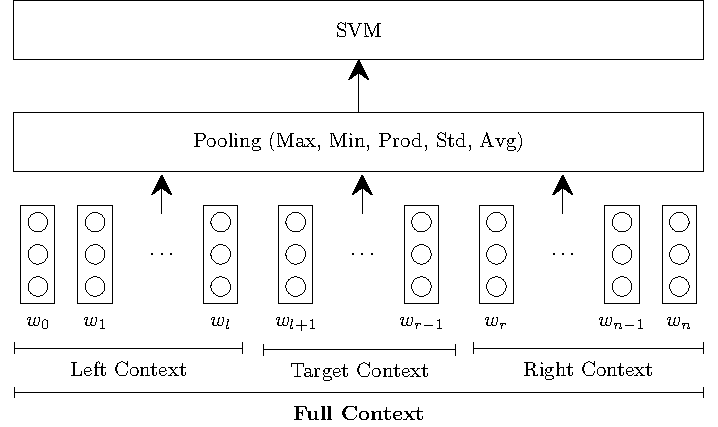
\includegraphics{Diagrams/Reproducibility/vo_method.pdf}
    \caption{General architecture of \citet{vo2015target} and \citet{wang-etal-2017-tdparse}.}
    \label{fig:repro_np_architecture}
\end{figure}
\newpage


%  sentence into different contexts to model simple interaction between the different contexts.
\subsection{Neural Pooling with Dependency Parsing}
\citet{wang-etal-2017-tdparse} method is a direct extension of \citet{vo2015target} where they keep the same NP methods and general architecture but change the contexts. The main motivation of \citet{wang-etal-2017-tdparse} is to improve the simple interaction of the different contexts by incorporating the syntactic structure of the target word using a dependency parser. In more detail this dependency context contains the target word and all connected words within the same root. This makes the assumption that the dependency parser that is used can create multiple roots from one text as it assumes the text is made of more than one sentence. If the dependency parser does not create more than one root in a text then the dependency context will be the same as the whole context\footnote{More precisely it will be the same as the whole context with the target word(s) removed, so very similar to the whole context. A python notebook demonstrating the fact that the authors used the dependency parser (TweeboParser) like this and if another parser is used e.g. Stanford the dependency context will be similar to the whole context can be found here: \url{https://github.com/apmoore1/Bella/blob/master/notebooks/tdparse\_parser.ipynb}.} from \citet{vo2015target} method. The dependency parser they therefore used was the TweeboParser \citep{kong-etal-2014-dependency}\footnote{To the author's knowledge it is believed TweeboParser is the only dependency parser that creates multiple roots for a given text. However the author is not an expert within the field of dependency parsing.} which was created for noisy text such as Tweets and hence why multiple roots can occur in one text. This parser was also used because it was especially created for noisy text and the datasets that \citet{wang-etal-2017-tdparse} applied this method to were Twitter datasets. Thus one expects that this method will work best on social media type of texts as this method has been developed with this bias.

As with \citet{vo2015target}, \citet{wang-etal-2017-tdparse} had three different models each containing either more contexts or external information, these are describe in more detail below:

\begin{enumerate}
    \item TDParse Minus -- Only used the dependency context.
    \item TDParse -- Left, right, target, and dependency contexts.
    \item TDParse Plus -- Left, right, target, dependency, \textit{LS}, and \textit{RS} contexts.
\end{enumerate}

Overall the general architecture of \citet{wang-etal-2017-tdparse} is in essence the same as that of \citet{vo2015target}, thus can then be summarised through figure \ref{fig:repro_np_architecture}. 

\subsection{LSTM}
\label{section:repro_lstm_description}
%[I may need the reference to the LSTM cell???]
Unlike the previous two methods this is a NN method, and it was the first for TDSA to use a LSTM. Similar to the other two methods \citet{tang-etal-2016-effective} created three different methods: 

\begin{enumerate}
    \item Standard LSTM (LSTM).
    \item Target Dependent LSTM (TDLSTM).
    \item Target Connected LSTM (TCLSTM).
\end{enumerate}

The LSTM method is the most basic approach and can be seen in full in figure \ref{fig:repro_lstm_method}. It treats each word within the text as a word vector where the word vector can be either randomly initialised or initialised from a pre-trained word embedding like GloVe. The word vectors are then inputted into the LSTM NN which takes the word vectors from the left most word first to the last word in the sentence. The output from the LSTM at the last word in the sentence ($h_n$) is fed into a linear layer with a softmax activation function to generate the probability of the sentiment of the text. This approach takes no target context into account, therefore it represents a sentence level sentiment classifier, and was used as the baseline method.

\begin{figure}[!h]
    \centering
    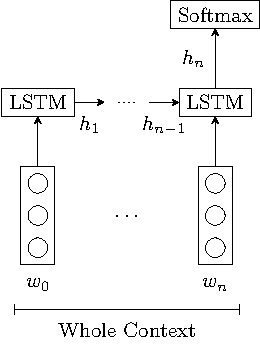
\includegraphics{Diagrams/Reproducibility/tang_lstm.pdf}
    \caption{Architecture of the LSTM method.}
    \label{fig:repro_lstm_method}
\end{figure}

The TDLSTM which can be seen in figure \ref{fig:repro_tdlstm_method}, it is a target specific model, it splits the sentence into two contexts:
\begin{enumerate}
    \item Left context -- The words left of the target word, including the target itself.
    \item Right context -- The words right of the target word, including the target itself.
\end{enumerate}
Each context has its own LSTM, the left has an LSTM that takes words vectors from left to right, and the right LSTM takes words vectors from right to left. The last word vector(s) that are input into both LSTMs are the target words, this was so that the LSTM could better model the sentiment of the sentence with regard to the target word(s). The final output of both LSTMs ($h_{r-1}$, $h_{l+1}$) are concatenated together, which is fed into a linear layer with a softmax activation function to generate the probability of the sentiment of the text.

\begin{figure}[!h]
    \centering
    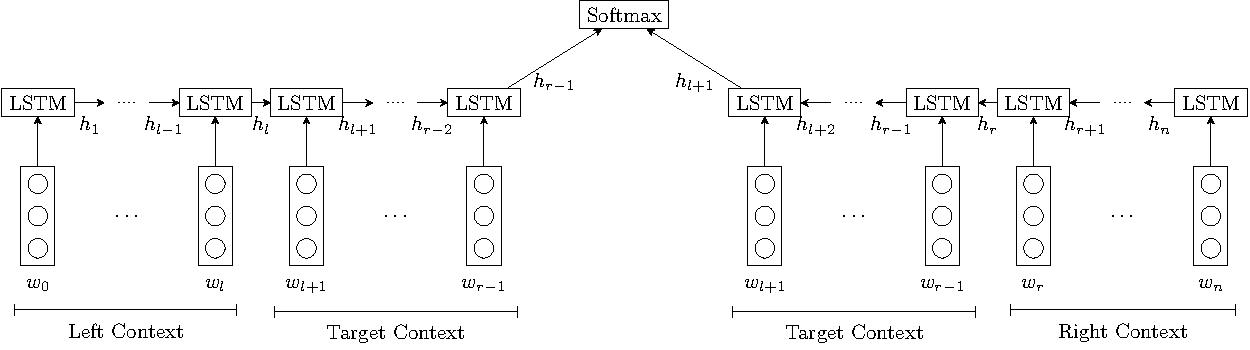
\includegraphics[scale=0.55]{Diagrams/Reproducibility/tang_tdlstm.pdf}
    \caption{Architecture of the TDLSTM method.}
    \label{fig:repro_tdlstm_method}
\end{figure}

Finally the TCLSTM method which can be seen in figure \ref{fig:repro_tclstm_method} is a direct extension of TDLSTM with only one minor difference. The difference is the concatenation of the target word vector ($t$) to each word vector within the text. The target word vector is represented as the average of all the target word vectors when the target word is made up of more than one word.

\begin{figure}[!h]
    \centering
    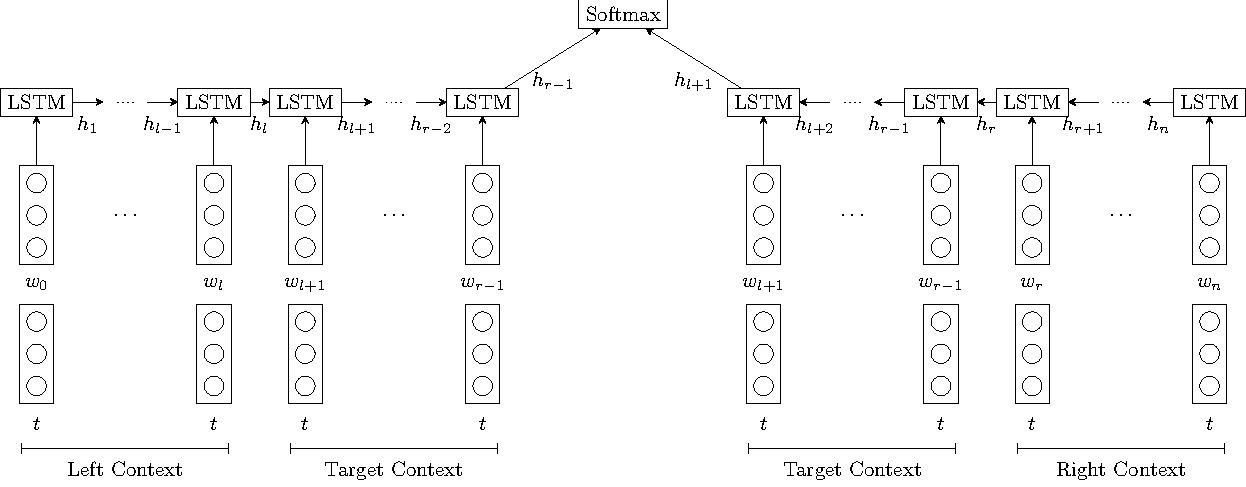
\includegraphics[scale=0.55]{Diagrams/Reproducibility/tang_tclstm.pdf}
    \caption{Architecture of the TCLSTM method.}
    \label{fig:repro_tclstm_method}
\end{figure}

%\subsection{Review of the three methods}
%The reason these three methods were chosen is two fold; first they can be split by the classifier the method uses, either a linear SVM or non linear NN, of which even though they have been compared before \cite{tang-etal-2016-effective, wang-etal-2017-tdparse} they have not been compared on datasets that are not Twitter based. Secondly \citet{vo2015target} and \citet{wang-etal-2017-tdparse} are very similar with the only difference being the whole and dependency contexts therefore it would be interesting to see if the dependency context is of importance generally across datasets that are not Twitter based.


\section{TDSA Reproduction Studies}
\label{section:repro_replication}

These studies will explore how the results from the original methods differ with those reproduced. Each paper will have its own subsection detailing the differences and if the differences are statistically significant. Furthermore, at the end of the section based on the results, suggestions are offered to make papers more reproducible. Lastly based on the reproduction results of \citet{tang-etal-2016-effective} additional suggestions are made for NN based methods to improve reporting of results, which in itself helps with both evaluation and reproducibility. A paper is defined as being reproduced if the main result is not statistically significantly different on at least one metric and if the results have the same rank order e.g. model A is better than model B for at least one metric. In the thesis, this is how the definition for reproducibility from the introduction \ref{section:repro_intro} has been empirically interpreted. Before conducting the reproducibility studies, the experimental setup for all of these studies will be stated defining the metrics, datasets, pre-processing steps, and how the statistical significance tests will be performed.

%The replication cases here will show that the methods recreated within this thesis can successfully replicate the experiments conducted within the papers of the three methods stated in section \ref{section:repro_methods}. The success is shown through the replicated methods to be not statistically different to the original methods on at least one of the metrics used. The importance of having accurately replicated methods is to allow the findings within the mass evaluation \ref{section:repro_mass_eval} and effects of parameter and experimental settings \ref{section:repro_effect_param_settings} sections to be valid and representative of the original method. This section will first explain how the experiments are setup and iteratively go through each of the three methods demonstrating that each has been successfully replicated.

%This section will demonstrate that the three methods stated above in the methods section \ref{section:repro_methods} are successfully replicated using significance testing. The section will start with a description of the significance test used in all the experiments, followed by a experiment(s) for each of the three methods to show that the methods have been successfully replicated.

%We now demonstrate through replicating the experiments in each paper and using statistical test that we have successfully replicated all of the methods.\\

% This might be better placed in the generlisation section/ dataset explaination section.
%
% This in itself is a bad dataset to be used for TDSA as there is only one unique target per sentence which can be seen in table \ref{table:repro_datasets_stats}. Even though the sentiment is with respect to the target and not the sentence you would not get issues such as conflicting sentiments within the sentence due to different targets having different sentiment. For example `The camera is very good but the lens is awful' would have two targets with conflicting sentiments.\\
% Type I error refers to the case where the null hypothesis is rejected when it is actually true. Type II error refers to the case where the null hypothesis is not rejected although it should be. A

%The methods within this subsection all use the general domain Twitter dataset from \cite{dong-etal-2014-adaptive}, \cite{wang-etal-2017-tdparse} also used their own political Twitter dataset. The pre-processing across all of the experiments is the same. We follow \cite{vo2015target} which is to lower case all text and tokenise using Twokenizer \cite{gimpel-etal-2011-part}. This process was used as the other papers do not explicitly state their pre-processing method. Furthermore the word embeddings used in all of the tests only contain lower cased words and the Twokenizer tokeniser is Twitter specific, thus justifying this pre-processing method.
\subsection{Experimental Setup}
\label{section:repro_experimental_setup}

Within the reproduction and mass evaluation experiments the following datasets will be used: 

\begin{enumerate}
    \item Laptop -- SemEval 2014 laptop dataset \citep{pontiki-etal-2014-semeval}.
    \item Restaurant -- SemEval 2014 restaurant dataset \citep{pontiki-etal-2014-semeval}.
    \item Mitchell -- English Twitter dataset \citep{mitchell-etal-2013-open}\footnote{The reason for specifying English is due to \citet{mitchell-etal-2013-open} also releasing a Spanish Twitter dataset within the same paper.}.
    \item Dong -- Twitter dataset \citep{dong-etal-2014-adaptive}.
    \item Election -- Election Twitter dataset \citep{wang-etal-2017-tdparse}.
    \item YouTuBean -- Captions from YouTube review videos \citep{marrese-taylor-etal-2017-mining}.
\end{enumerate}

Table \ref{table:repro_dataset_stats} provides a description of the datasets, of which the YouTuBean is by far the smallest dataset. Further the sentiment class and Distinct Sentiment (\textit{DS}) distributions can be seen in table \ref{table:repro_dataset_sent_dist}. The \textit{DS} \citep{wang-etal-2017-tdparse} is based around the number of unique sentiments per text: $DS_1$, $DS_2$, and $DS_3$ would be all the samples that contain only one, two, and three sentiments in the text, respectively. The idea behind showing the \textit{DS} is a way of judging potentially how difficult a dataset is going to be where the larger $i$ in $DS_i$ the more difficult the dataset might be\footnote{In chapter \ref{chapter:methodology} it is shown empirically that the large $i$ is within $DS_i$ the more difficult it will be to classify the samples within that distribution.}. Thus from both tables it is clear to see that the datasets are all very different with some being heavily unbalanced with respect to sentiment class distribution (Mitchell). 

\begin{table}[!h]
    \centering
    \begin{tabular}{|c|c|c|c|c|c|c|c|}
\hline
Dataset & DO & T & M & No. Targets & ATS & Uniq & AVG Len \\
 \hline
Laptop & L & RE & W & 2951 & 1.58 & 1295 & 18.57  \\
\hline
Restaurant & R & RE & W & 4722 & 1.83 & 1630 & 17.25  \\
\hline
Mitchell & G & S & W & 3288 & 1.22 & 2507 & 18.02 \\
\hline
Dong & G & S & W & 6940 & 1.00 & 145 & 17.37 \\
\hline
Election & P & S & W & 11899 & 2.94 & 2190 & 21.68 \\
\hline
YouTuBean & MP & RE\slash S & SP & 798 & 2.07 & 522 & 22.53 \\
\hline
\multicolumn{8}{|p{0.95\linewidth}|}{L=Laptop, R=Restaurant, P=Politics, MP=Mobile Phones, G=General, T=Type, RE=Review, S=Social Media, ATS=Average targets per sentence, Uniq=No. unique targets, AVG len=Average sentence length per target, DO=Domain, M=Medium, W=Written, SP=Spoken}\\
\hline
\end{tabular}
    \caption{Dataset descriptions and size statistics.}
    \label{table:repro_dataset_stats}
\end{table}

\begin{table}[!h]
    \centering
    \begin{tabular}{|c|c|c|c|c|c|c|}
        \hline
        Dataset & Pos \sd{(\%)} & Neu \sd{(\%)} & Neg \sd{(\%)} & $DS_1$ & $DS_2$ & $DS_3$ \\
        \hline
        Laptop & 1328 \sd{(45)} & 629 \sd{(21.3)} & 994 \sd{(33.7)} & 81\% & 18\% & 1\% \\
        \hline
        Restaurant & 2892 \sd{(61.3)} & 829 \sd{(17.6)} & 1001 \sd{(21.2)} & 75\% & 23\% & 2\% \\
        \hline
        Mitchell & 707 \sd{(21.5)} & 2306 \sd{(70.1)} & 275 \sd{(8.4)} & 91\% & 9\% & 0\% \\
        \hline
        Dong & 1734 \sd{(25)} & 3473 \sd{(50)} & 1733 \sd{(25)} & 100\% & 0\% & 0\% \\
        \hline 
        Election & 1744 \sd{(14.7)} & 4572 \sd{(38.4)} & 5583 \sd{(46.9)} & 44\% & 47\% & 9\% \\
        \hline 
        YouTuBean & 224 \sd{(28.1)} & 504 \sd{(63.2)} & 70 \sd{(8.8)} & 82\% & 18\% & 0\% \\
        \hline
        \multicolumn{7}{|p{0.85\linewidth}|}{Pos=Number of positive targets, Neu=Number of neutral targets, Neg=Number of negative targets, $DS_1$=1 Distinct Sentiment per sentence, $DS_2$=2 Distinct Sentiments per sentence, $DS_3$=3 Distinct Sentiments per sentence}\\
        \hline
\end{tabular}
    \caption{Dataset sentiment class and distinct sentiment distributions.}
    \label{table:repro_dataset_sent_dist}
\end{table}

The Dong dataset\footnote{This dataset can be downloaded from \url{http://goo.gl/5Enpu7}.} is a special case out of all of the datasets, as even though it has been used in previous research as shown in table \ref{table:repro_methods_datasets_used}, it is not a true TDSA dataset. The dataset is more of an Aspect Based Sentiment Analysis dataset as the annotation gives the target and all of its occurrences in the text, rather than just the relevant target occurrence. Example \ref{example:repro_dong_data_example} is from the training dataset, where \$T\$ represents all of the places the target occurs in the text, and here it is clear that the first target (\$T\$) is not the target that is negatively affected rather it is the second target (\$T\$). This issue of not knowing which is the relevant target was denoted as ``same target multiple appearances'' by \citet{wang-etal-2017-tdparse}. Thus when using the Dong dataset for the \citet{tang-etal-2016-effective} methods the first target (\$T\$) is assumed to be the relevant target in all cases, and when using the NP approaches the feature vector of all target occurrences are median pooled which is the approach used by \citet{wang-etal-2017-tdparse}. It is not clear how either \citet{vo2015target} or \citet{tang-etal-2016-effective} handled the `same target multiple appearance' issue.

\begin{example}
\textit{\$T\$ has brought back the female rapper . - really ? \$T\$ is the biggest parody in popular music since the Lonely Island .}
\caption{An example from the training dataset of Dong \citep{dong-etal-2014-adaptive}, where \$T\$ is a placeholder for the target `nicki minaj'. The sentiment towards the target is negative.}
\label{example:repro_dong_data_example}
\end{example}

As stated earlier, to test if the method has been successfully reproduced the results from the reproduced method will not be statistically significantly different to the original method's results. To choose an appropriate statistical test, the guide from \citet{dror-etal-2018-hitchhikers} has been followed, from which the non-parametric paired bootstrap test \citep{efron_1993} has been selected. This was chosen as the distribution of results cannot always be assumed to come from a normal distribution, due to the macro F1 metric \citep{dror-etal-2018-hitchhikers} which is one of the metrics used within the experiments. Thus this breaks the assumptions of the more powerful parametric tests (student's t-test). Furthermore, out of the two families of non-parametric tests the sampling-based tests are more powerful \citep{dror-etal-2018-hitchhikers, sogaard-etal-2014-whats} (fewer type 2 errors\footnote{Type 2 error: `refers to the case where the null hypothesis is not rejected although it should be.'\citep{dror-etal-2018-hitchhikers}}), from this either Pitman's permutation test or the paired bootstrap can be used, thus we follow \citet{sogaard-etal-2014-whats} in using the paired bootstrap test. The one assumption that has to be made with the paired bootstrap is that the test data is representative of the overall population by having a large enough test set size. Therefore we take the suggestion from \citet{sogaard-etal-2014-whats} and assume that a test set of size greater than 200 is enough to ensure the type 1 errors\footnote{Type 1 error: `refers to the case where the null hypothesis is rejected when it is actually true.'\citep{dror-etal-2018-hitchhikers}} are minimised. The only experiments that cannot assume the test size is greater than 200 are those that apply five-fold cross validation on the YouTuBean dataset.

%For one of the metrics (accuracy) it can be assumed that the results have come from a normal distribution \citep{dror-etal-2018-hitchhikers}. However as the number of results created from the NP methods when evaluated purely on the test sets will be one, one result is not a distribution of results. Thus for any of the parametric tests to work a large enough sample of results is needed, which is at least greater than one. Hence another reason why the parametric tests cannot be used even for results that come from a metric that can be assumed to come from a normal distribution, like in this case accuracy.

%To further explain why our results will not follow a normal distribution, this is due to the two metrics that are used through out most of the experiments. The two metrics are the macro F1 score and accuracy, results from the accuracy metric can be assumed to be normal if the number of predictions is large enough \citep{dror-etal-2018-hitchhikers}. However considering the minimum number of scores produced for each experiment will be 1 this would not be considered `large enough' thus a normal distribution cannot be assumed for the accuracy metric. %Also within the reproduction case of \citet{tang-etal-2016-effective} it is shown by using the Shapiro-Wilk test \citep{shapiro1965analysis} for normality (which is the recommended test within \citet{dror-etal-2018-hitchhikers}) that not all accuracy metric scores come from a normal distribution. Thus as it cannot be assumed that all accuracy scores come from a normal distribution and F1 scores have not be shown too either, we assume the results will not follow a normal distribution.

The metrics used in all the experiments will be both the accuracy and macro F1 scores as these are the most frequently used metrics within TDSA \citep{dong-etal-2014-adaptive,wang-etal-2017-tdparse,he-etal-2018-exploiting}. The accuracy score can be calculated using equation \ref{eq:repro_accuracy} where $TP$ refers to the number of correctly labelled samples and $N$ are the number of samples in the dataset. The macro F1 score can be calculated using equation \ref{eq:repro_macro_f1} where the $F1(pos)$, $F1(neu)$, and $F1(neg)$ is the F1 score for the positive, neutral, and negative classes respectively. One of the differences between the two is that the accuracy score is performed globally and thus does not discriminate based on the class label, whereas the macro F1 does as it has to calculate the F1 score for each class and then perform an un-weighted average across all three classes. Due to the un-balanced nature of class labels within all of the TDSA datasets, as shown in table \ref{table:repro_dataset_sent_dist}, the macro F1 score is more biased towards methods that perform well across all sentiments rather than just the dominant sentiment. In comparison, the accuracy score can still be very high with just predicting the most dominant sentiment all of the time. Finally the majority baseline for accuracy will always be greater than that of the macro F1 due to the un-weighted averaging over the sentiment classes. Thus in general the macro F1 score is a harder metric. The two metrics allows for fair comparison with other works in the community.

\begin{equation}
    Accuracy = \frac{TP}{N}
    \label{eq:repro_accuracy}
\end{equation}
\begin{equation}
    F1 = 2 * \frac{Recall * Precision}{Recall + Precision}
\end{equation}
\begin{equation}
    Macro\, F1 = \frac{F1(pos)\, +\, F1(neu)\, + \, F1(neg)}{3}
    \label{eq:repro_macro_f1}
\end{equation}

The null hypothesis that is being tested within this reproduction section is the following: 
\begin{hyp}
The reproduced method (R) is no better or worse than the original method (O) on a given population x\footnote{x is defined later on in this section.}. 
\label{hyp:repro_replication_null}
\end{hyp}
While the alternative is:
\begin{hyp}
The reproduced method (R) is better or worse than the original method (O) on a given population x. 
\label{hyp:repro_replication_alt}
\end{hyp}
The null hypothesis \ref{hyp:repro_replication_null} will be tested using a two tailed test as it is to be seen if the reproduced method is better or worse rather than just one of those options otherwise a one tailed test would be used. This null hypothesis can be expressed through equations \ref{eq:repro_null_hypo_better} and \ref{eq:repro_null_hypo_worse}, where $\delta(x)$ is expressed in equation \ref{eq:repro_score_diff} and $M$ represents an evaluation metric of which this would be either accuracy or macro F1.

\begin{equation}
    p(\delta(X\footnote{X is defined later on in this section.}) \leq 0)
\label{eq:repro_null_hypo_better}
\end{equation}

\begin{equation}
    p(\delta(X) \geq 0)
\label{eq:repro_null_hypo_worse}
\end{equation}

\begin{equation}
    \delta(x) = M(R(x)) - M(O(x))
\label{eq:repro_score_diff}
\end{equation}

To reject the null hypothesis \ref{hyp:repro_replication_null} and accept the alternative hypothesis \ref{hyp:repro_replication_alt} equation \ref{eq:repro_null_diff_better} or \ref{eq:repro_null_diff_worse} has to be true for some given $\alpha$.
\begin{equation}
    p(\delta(X) \leq 0) \le \frac{\alpha}{2}
\label{eq:repro_null_diff_better}
\end{equation}
\begin{equation}
    p(\delta(X) \geq 0) \le \frac{\alpha}{2}
\label{eq:repro_null_diff_worse}
\end{equation}
The $\alpha$ value\footnote{It is suggested in \citet{sogaard-etal-2014-whats} that an $\alpha$ of 0.0025 should be used and that p-values are recorded.} determines the upper bound on the number of type 1 errors that can occur \citep{dror-etal-2018-hitchhikers}. Therefore in this thesis an $\alpha$ value of 0.05 is chosen as this is the most popular value used within the field \citep{liu-zhang-2017-attention,he-etal-2018-exploiting}.

The population $x$ is normally our test set when comparing two systems, and we assume that this test has come from a large population $X$. The null hypothesis is used to ensure that our one test score on the given test set $x$ has not come about by chance. Therefore to compute the p-value for equations \ref{eq:repro_null_hypo_better} and \ref{eq:repro_null_hypo_worse} we approximate the larger population $X$ using the bootstrap re-sampling method. This is a method of creating $Z$ test sets of size $n$, which is the same size as the original test set, by sampling from the test set with replacement. The assumption is that this creates new test sets that are representative but different from the original, which can be used as a proxy of the larger population $X$. The paired bootstrap procedure is presented in algorithm \ref{algo:repro_bootstrap}, which is used to approximate the p-values of which $p_0$ and $p_1$ can be substituted as the p-value in equations \ref{eq:repro_null_diff_better} and \ref{eq:repro_null_diff_worse}. For all experiments $Z$ is at least equal to 1000\footnote{In some cases where it was computationally feasible $Z$ was 10,000.}, which is the same as \citet{koehn-2004-statistical} used and is computational feasible. 

\begin{algorithm}
    Draw \textit{Z} bootstrap samples of size $n$ by sampling with replacements from $x$\;
    $w = 0$\;
    $b = 0$\;
    \For{each $x^{(i)}$ increment}{
        \uIf{$\delta(x^{(i)}) < 0$}
        {
            $w = w + 1$\;
        }
        \uIf{$\delta(x^{(i)}) > 0$}
        {
            $b = b + 1$\;
        }
    }
    $p_0$ $\approx 1 - \frac{w}{Z}$\;
    $p_1$ $\approx 1 - \frac{b}{Z}$\;
    return $p_0$ and $p_1$\;
    \caption{The paired bootstrap algorithm adapted from figure 1 in \citet{berg-kirkpatrick-etal-2012-empirical}}
    \label{algo:repro_bootstrap}
\end{algorithm}

This bootstrapping approach can therefore be used to create a confidence range for a method whereby using these $Z$ metric scores as a distribution of results. From this distribution removing the top and bottom 2.5\% of scores creates the confidence range for an $\alpha=0.05$\footnote{The percentage to remove is equal to $\frac{\alpha}{2} \times 100$ for the two tailed test.}, for the two tailed test, as shown by \citet{koehn-2004-statistical}. If the reproduced confidence range does not include the original method's score the null hypothesis must be rejected. 

The two tailed test can easily be converted into a one tailed test, to test if a method is better than another, whereby the hypothesis now changes to:
\begin{hyp}
Reproduced method A is no better than the original method B on a given population x. 
\label{hyp:repro_replication_better_null}
\end{hyp}
While the alternative is:
\begin{hyp}
Reproduced method A is better than the original method B on a given population x. 
\label{hyp:repro_replication_better_alt}
\end{hyp}

The null hypothesis \ref{hyp:repro_replication_better_null} can be expressed by equations \ref{eq:repro_null_hypo_worse} and \ref{eq:repro_score_better_diff}.  

\begin{equation}
 \delta(x) = M(A(x)) - M(B(x))
\label{eq:repro_score_better_diff}
\end{equation}

To reject this null hypothesis \ref{hyp:repro_replication_better_null} equation \ref{eq:repro_null_diff_better_worse} has to be true for some $\alpha$, which in this thesis is $0.05$. 
\begin{equation}
    p(\delta(X) \geq 0) \le \alpha
\label{eq:repro_null_diff_better_worse}
\end{equation}

The pre-processing for the two NP approaches will use the Twitter based tokeniser; Twokenizer \citep{gimpel-etal-2011-part} as this was stated within \citet{vo2015target} and is shown to be used within \citet{wang-etal-2017-tdparse} codebase\footnote{\url{https://github.com/bluemonk482/tdparse/blob/master/data/dataprocessing.py}}. For the LSTM approach \citep{tang-etal-2016-effective} the English Spacy tokeniser is used due to its speed and wide use within the NLP field, as well as \citet{tang-etal-2016-effective} not stating the tokeniser used. All text is lower cased after being tokenised.

For the NP methods scikit-learn's \citep{pedregosa2011scikit} LinearSVC is used as it is a wrapper of LibLinear \citep{fan2008liblinear} which is the library that both NP papers original used for their SVMs. For \citet{tang-etal-2016-effective} LSTM based methods the AllenNLP framework \citep{gardner-etal-2018-allennlp} is used which uses PyTorch \citep{NEURIPS2019_9015}. 



\subsection{Neural Pooling}
\label{section:repro_neural_pooling}
To state if the paper \citep{vo2015target} has been reproduced the last experiment in the paper (table 5 \citep{vo2015target}) is performed which evaluates the methods on the test set of \citet{dong-etal-2014-adaptive} Twitter dataset. To be comparable the same SVM C-value parameters are used for all methods and sentiment lexicons for the Target-Dependent Plus method. Also the same word vectors are used which are the concatenation of the unified Sentiment Specific Word Embeddings (SSWE) \citep{tang-etal-2014-learning} and their own Twitter specific continuous skip-gram \citep{mikolov2013efficient} word vectors (w2v) creating SSWE + w2v. Finally MinMax scaling, as shown in equation \ref{eq:repro_min_max_scaling}, is used on all features, whereby this enforces a feature to be in a pre-defined \textit{max} to \textit{min} range for all samples ($X \in \R^{n \times d}$ where $n$ is the number of samples and $d$ is the number of features). This therefore enforces all features to be within the same range and ``avoid attributes (features) in greater numeric ranges dominating those in smaller numeric ranges'' \citep{hsu2003practical}. $X_{min} \in \R^d$ and $X_{max} \in \R^d$ are the smallest and largest value respectively for each feature. Within this thesis the \textit{min} and \textit{max} will be $0$ and $1$ respectively as this is one of the recommended ranges by \citet{hsu2003practical}. Only after the experiments have been conducted within this thesis, after looking through \citet{wang-etal-2017-tdparse} codebase, was it found they used $-1$ and $1$ for \textit{min} and \textit{max}. Thus it will be shown the difference between using these two different \textit{min} and \textit{max} ranges is negligible.

\begin{equation}
    X = \frac{X - X_{min}}{X_{max} - X_{min}} * (max - min) + min
    \label{eq:repro_min_max_scaling}
\end{equation}

The results from this experiment can be seen in table \ref{table:repro_vo_main_results} which compares the reproduced to the original. The original did not use the Target-Dependent Minus method within this experiment. As can be seen the results are similar to the original. However by adding only target context information and removing the whole text context (Target-Dependent Minus) does not improve results greatly over the standard non-target aware method (Target-Independent). Further Target-Dependent Minus is not statistically significantly better than Target-Independent on either of the two metrics, as shown by the p-values in table \ref{table:repro_vo_main_results_p_values}. Thus showing for the first time that adding the whole text context is statistically significant within the Target-Dependent method and not just on average better, as shown by table \ref{table:repro_vo_main_results_p_values}. Figure \ref{fig:repro_vo_Target_Reproduction_Dong} shows the confidence intervals of each reproduced method, and that for the accuracy metric all of the original results are within confidence intervals. Further according to the results all methods are in the same rank order as the original. Thus this paper has been reproduced.

\FloatBarrier
\begin{table}[!h]
    \centering
    \begin{tabular}{|c|c|c|c|c|}
 \hline
 & \multicolumn{2}{c|}{Accuracy} & \multicolumn{2}{c|}{macro F1} \\
 \hline
 Model & O & R & O & R \\ 
 \hline
 Target Independent     &     67.3 &         65.0 &     66.4 &         61.9 \\
 \hline
 Target Dependent Minus &      0.0 &         66.6 &      0.0 &         62.1 \\
 \hline
 Target Dependent       &     69.7 &         69.7 &     68.0 &         66.7 \\
 \hline
 Target Dependent Plus  &     71.1 &         69.9 &     69.9 &         67.6 \\
\hline
\end{tabular}
    \caption{Reproduced (R) and original (O) results on the test set of \citet{dong-etal-2014-adaptive} Twitter dataset.}
    \label{table:repro_vo_main_results}
\end{table}
\FloatBarrier

\FloatBarrier
\begin{table}[!h]
    \centering
    \begin{tabular}{|c|c|c|c|c|c|}         
\hline
Metric &    Method                   &  TI &  TDM &  TD &  TDP \\
\hline
\multirow{4}{*}{macro F1} & TI &              - &                  0.5459 &            0.9976 &                 0.9995 \\
& TDM &              0.4541 &                  - &            0.9995 &                 0.9994 \\
& TD &              \textbf{0.0024} &                  \textbf{0.0005} &            - &                 0.7606 \\
& TDP &              \textbf{0.0005} &                  \textbf{0.0006} &            0.2394 &                 - \\
\hline
\multirow{4}{*}{Accuracy} & TI &              - &                  0.8245 &            0.9987 &                 0.9986 \\
& TDM &              0.1962 &                  - &            0.9935 &                 0.9905 \\
& TD &              \textbf{0.0017} &                  \textbf{0.0094} &            - &                 0.6284 \\
& TDP &              \textbf{0.0019} &                  \textbf{0.0121} &            0.4223 &                 - \\
\hline
\end{tabular}
    \caption{P-values testing if the methods in the rows are significantly better than the methods in the columns across two metrics. All p-values that are significant $\le 0.05$ are in \textbf{bold}.}
    \label{table:repro_vo_main_results_p_values}
\end{table}
\FloatBarrier

\begin{figure}[!h]
    \centering
    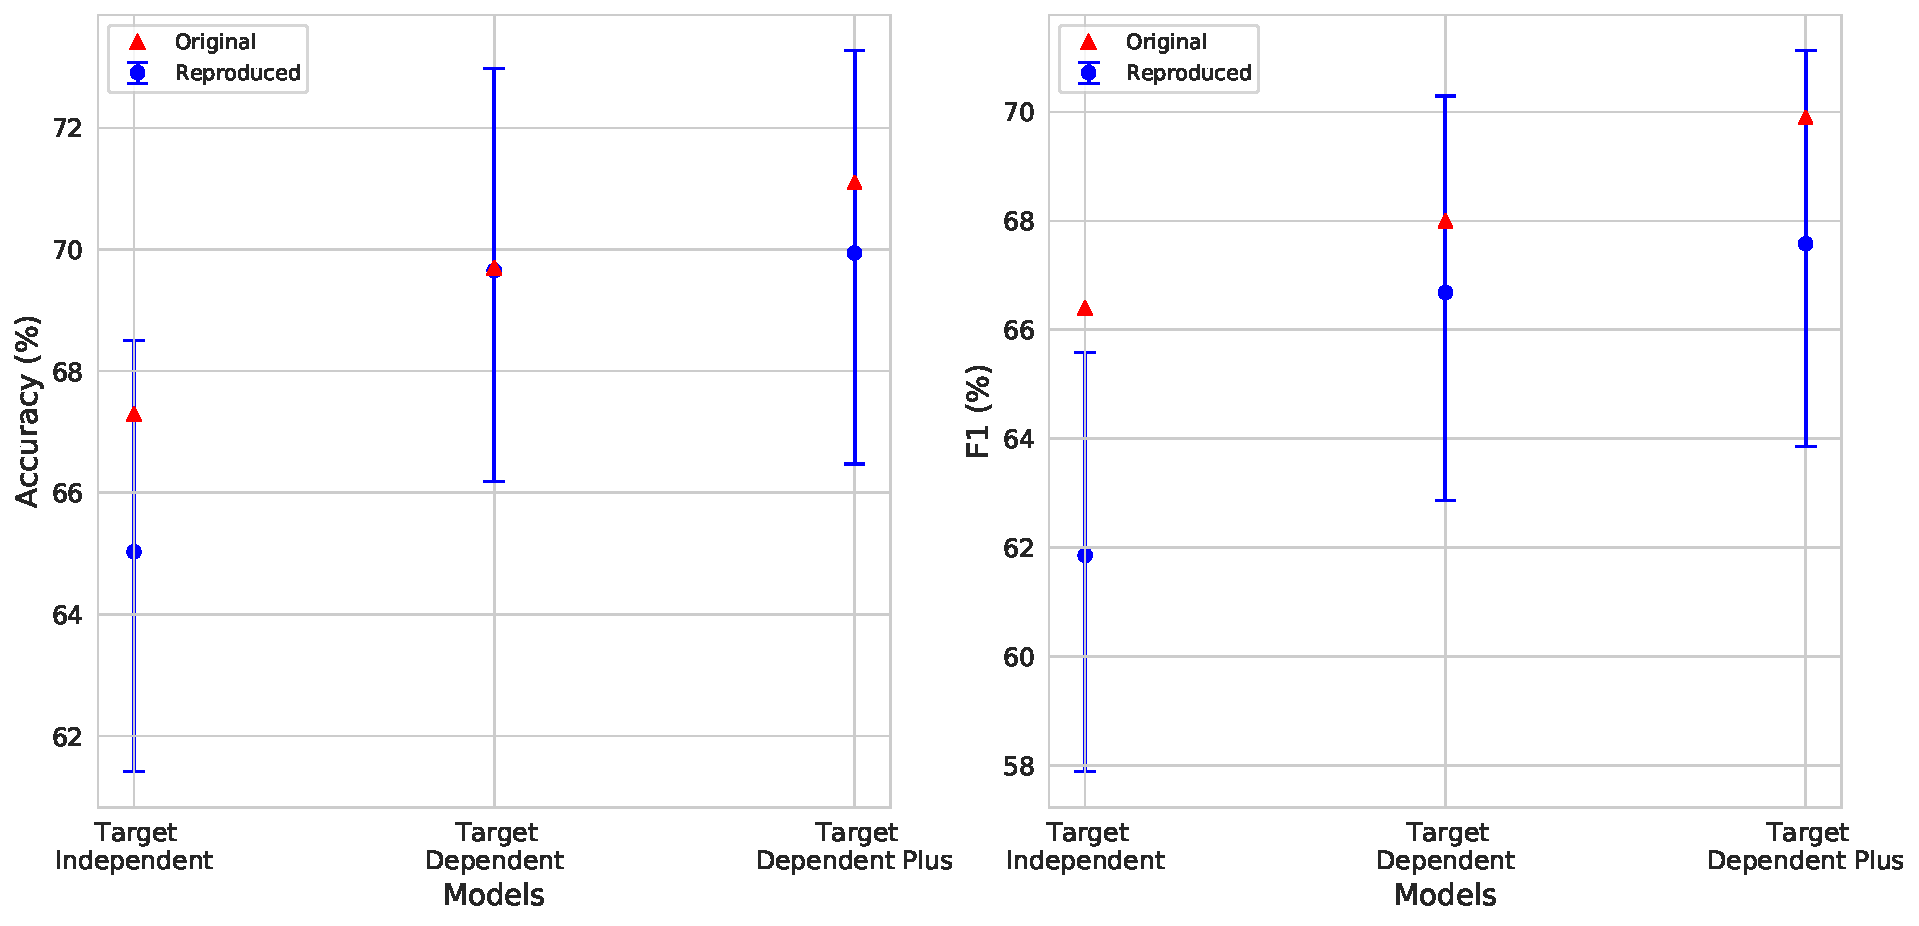
\includegraphics[scale=0.37]{images/reproducibility/vo/Target_Reproduction_Dong.pdf}
    \caption{Confidence intervals for the two tailed test for the reproduced models of \citet{vo2015target} on both the accuracy and macro F1 metrics.}
    \label{fig:repro_vo_Target_Reproduction_Dong}
\end{figure}

As stated earlier \citet{wang-etal-2017-tdparse} used a different scaling range, $-1$ to $1$, for MinMax scaling. Figure \ref{fig:repro_vo_Target_Wang_Scaled_Reproduction_Dong} shows the confidence intervals for each method when using \citet{wang-etal-2017-tdparse} scaling range on the test set of \citet{dong-etal-2014-adaptive} Twitter dataset. As can be seen the confidence intervals would overlap with those from figure \ref{fig:repro_vo_Target_Reproduction_Dong} which used the $0$ to $1$ scaling range that is used throughout the Neural Pooling experiments. Thus showing in this case the scaling range would not appear to be a significant factor.

\begin{figure}[!h]
    \centering
    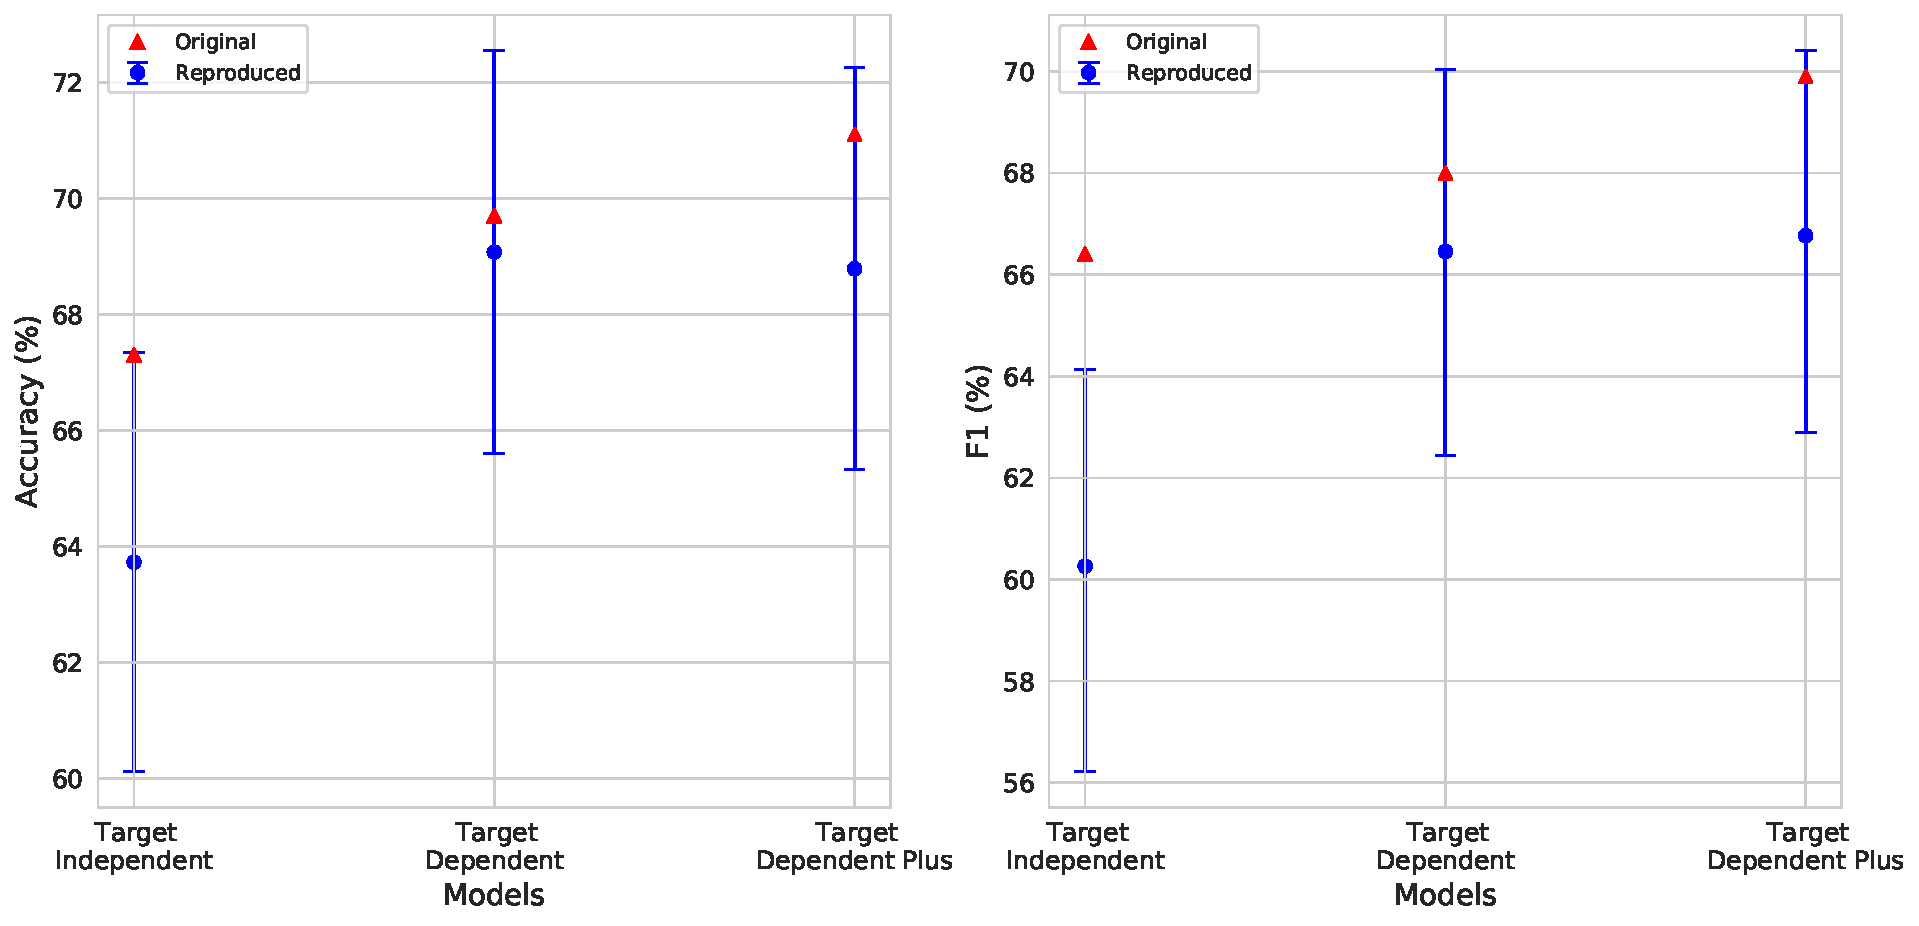
\includegraphics[scale=0.37]{images/reproducibility/vo/Target_Wang_Scaled_Reproduction_Dong.pdf}
    \caption{Confidence intervals for the two tailed test for the reproduced models of \citet{vo2015target} using \citet{wang-etal-2017-tdparse} scaling range of $-1$ to $1$, on both the accuracy and macro F1 metrics.}
    \label{fig:repro_vo_Target_Wang_Scaled_Reproduction_Dong}
\end{figure}

Given that the paper has been reproduced, further studies are explored. The first of which is comparing different word embeddings, in \citet{vo2015target} they compared w2v, SSWE, and SSWE + w2v. The comparison was done using five-fold cross validation on the training data whereby they report the mean accuracy scores within figure 4 of their paper. This experiment has been recreated, and the word embeddings compared have been expanded to include the non-type non-task specific 300 dimension 840 billion token GloVe embeddings \citep{pennington-etal-2014-glove} (from now on called GloVe embeddings). These much larger word embeddings are by the far the most popular embeddings within the TDSA literature. Furthermore unlike w2v which are type specific and SSWE which are task and type specific these are neither and more general. Thus it would be of interest to see if general embeddings can perform as well or better than the original task and type specific embeddings. The results of the experiment can be seen in table \ref{table:repro_vo_word_embeddings_results}. As can be seen the GloVe and the SSWE + w2v are very similar in their performance, and both always outperform the w2v and SSWE embeddings. However unlike the original results, the reproduced results tend to find w2v to perform better than SSWE, as shown by the highlighting in the table.  

\FloatBarrier
\begin{table}[!h]
    \centering
    \begin{tabular}{|c|c|M|M|c|M|}
\hline
&  & \multicolumn{2}{c|}{Accuracy} & \multicolumn{2}{c|}{macro F1} \\
\hline
Method & Embedding &      O &  R &     O &  R \\
\hline
\multirow{4}{*}{TI} & w2v &  59.20 \sd{(0.00)} &  \highbox{60.96} \sd{(0.60)} &  - &  56.64 \sd{(0.69)} \\
& SSWE &  60.70 \sd{(0.00)} &  \highbox{60.58} \sd{(1.08)} &  - &  56.52 \sd{(1.46)} \\
& SSWE + w2v &  62.30 \sd{(0.00)} &  62.24 \sd{(0.91)} &  - &  59.16 \sd{(0.66)} \\
& GloVe &   - &  \textbf{63.72} \sd{(1.76)} &  - &  \textbf{61.31} \sd{(1.74)} \\
\hline
\multirow{4}{*}{TDM} & w2v &  65.40 \sd{(0.00)} &  65.67 \sd{(1.11)} &  - &  61.38 \sd{(1.29)} \\
& SSWE &  66.60 \sd{(0.00)} &  66.74 \sd{(0.48)} &  - &  62.77 \sd{(0.78)} \\
& SSWE + w2v &  67.60 \sd{(0.00)} &  \textbf{67.46} \sd{(1.04)} &  - &  \textbf{64.18} \sd{(1.18)} \\
& GloVe &   - &  67.41 \sd{(0.78)} &  - &  64.11 \sd{(0.82)} \\
\hline
\multirow{4}{*}{TD} & w2v &  65.70 \sd{(0.00)} &  \highbox{66.81} \sd{(0.86)} &  - &  62.66 \sd{(1.16)} \\
& SSWE &  66.70 \sd{(0.00)} &  \highbox{66.37} \sd{(0.59)} &  - &  62.41 \sd{(0.81)} \\
& SSWE + w2v &  68.30 \sd{(0.00)} &  68.02 \sd{(0.82)} &  - &  64.90 \sd{(0.91)} \\
& GloVe &   - &  \textbf{68.69} \sd{(1.13)} &  - &  \textbf{65.68} \sd{(1.24)} \\
\hline
\multirow{4}{*}{TDP} & w2v &  67.40 \sd{(0.00)} &  \highbox{68.37} \sd{(1.17)} &  - &  65.04 \sd{(1.39)} \\
& SSWE &  67.90 \sd{(0.00)} &  \highbox{67.72} \sd{(1.11)} &  - &  64.39 \sd{(1.54)} \\
& SSWE + w2v &  69.10 \sd{(0.00)} &  \textbf{69.05} \sd{(1.19)} &  - &  66.34 \sd{(1.41)} \\
& GloVe &   - &  68.98 \sd{(1.09)} &  - &  \textbf{66.39} \sd{(1.23)} \\
\hline
\end{tabular}
    \caption{Mean (standard deviation) metric score for each method and embedding, where the \textbf{bold} value represents the best embedding for each method and metric. Difference in rank order is \highbox{highlighted}.}
    \label{table:repro_vo_word_embeddings_results}
\end{table}
\FloatBarrier

These results for the embedding comparison so far has only been based on mean accuracy scores from five-fold cross validation. To be more rigorous in evaluation, significant testing is performed whereby the one tailed test is performed on each fold comparing the SSWE + w2v embedding score per metric and method to all other embeddings. The SSWE + w2v embedding was compared to the others as this was the best embedding from the original paper. The p-values generated from these significant tests can be seen in appendix \ref{appendix_reproducibility_tables} tables \ref{table:repro_vo_appendix_embedding_p_values_accuracy} and \ref{table:repro_vo_appendix_embedding_p_values_macro_f1} for the accuracy and macro F1 scores respectively. Furthermore as the significance testing is now performed on five folds, which is equivalent to five datasets, thus creating five p-values for each evaluation. Therefore here the number of folds that are significant will be reported. However using the simple approach of counting the number of folds that are less than some $\alpha$ has been shown to introduce more type 1 errors \citep{dror-etal-2017-replicability} than that was set by the $\alpha$ parameter, which is $0.05$, in the individual significance tests. Therefore to stop the introduction of type 1 errors and keep the upper bound to $\alpha$ a correction procedure is required of which \citet{dror-etal-2018-hitchhikers} recommends two; Fisher and Bonferroni \citep{benjamini2008screening}. The difference between the two is that Fisher should be used when the p-values have come from datasets that are independent, where as Bonferroni can be used for dependent datasets. As each fold does depend on the other folds, the Bonferroni correction will be used here. This thus introduces how significance testing can be performed in general for multiple datasets.

Table \ref{table:repro_vo_word_embedding_sig_fold_count} shows that for at least one of the folds, metric, and methods SSWE + w2v is significantly better than the SSWE and w2v embeddings but not the GloVe. Thus showing like the original paper that SSWE + w2v are the best embedding in general out of SSWE and w2v. Furthermore the GloVe embedding is also tested to see if it is better than the other embeddings using a one sided test and corrected using Bonferroni\footnote{The p-values associated to these tests can be seen in appendix \ref{appendix_reproducibility_tables} tables \ref{table:repro_vo_appendix_embedding_glove_accuracy_p_values} and \ref{table:repro_vo_appendix_embedding_glove_f1_p_values} for the accuracy and macro F1 metrics respectively.}, of which the results can be seen in table \ref{table:repro_vo_glove_embedding_sig_fold_count}. Thus from both experiments in tables \ref{table:repro_vo_word_embedding_sig_fold_count} and \ref{table:repro_vo_glove_embedding_sig_fold_count} it shows that the GloVe embedding is a reasonable replacement for the type and task specific combination of SSWE + w2v.

\begin{table}[!h]
    \centering
    \begin{tabular}{|c|c|c|c|}
\hline
Method &    Embedding   &  Accuracy &  F1 \\
\hline
\multirow{3}{*}{Target Independent} & w2v &         0 &   2 \\
& SSWE &         1 &   2 \\
& GloVe &         0 &   0 \\
\hline
\multirow{3}{*}{Target Dependent Minus} & w2v &         3 &   4 \\
& SSWE &         0 &   0 \\
& GloVe &         0 &   0 \\
\hline
\multirow{3}{*}{Target Dependent} & w2v &         0 &   4 \\
& SSWE &         0 &   2 \\
& GloVe &         0 &   0 \\
\hline
\multirow{3}{*}{Target Dependent Plus} & w2v &         0 &   0 \\
& SSWE &         1 &   1 \\
& GloVe &         0 &   0 \\
\hline
\end{tabular}
    \caption{The number of folds, out of a possible of five, that the SSWE + w2v embedding is significantly better than the given embedding and method. The significant testing across multiple folds is corrected using Bonferroni.}
    \label{table:repro_vo_word_embedding_sig_fold_count}
\end{table}

\begin{table}[!h]
    \centering
    \begin{tabular}{|c|c|c|c|}
\hline
Method &    Embedding   &  Accuracy &  F1 \\
\hline
\multirow{3}{*}{Target Independent} & w2v &         2 &   5 \\
& SSWE &         1 &   5 \\
& SSWE + w2v &         1 &   1 \\
\hline
\multirow{3}{*}{Target Dependent Minus} & w2v &         0 &   1 \\
& SSWE &         0 &   1 \\
& SSWE + w2v &         0 &   0 \\
\hline
\multirow{3}{*}{Target Dependent} & w2v &         1 &   4 \\
& SSWE &         3 &   4 \\
& SSWE + w2v &         0 &   0 \\
\hline
\multirow{3}{*}{Target Dependent Plus} & w2v &         0 &   0 \\
& SSWE &         0 &   1 \\
& SSWE + w2v &         0 &   0 \\ 
\hline
\end{tabular}
    \caption{The number of folds, out of a possible of five, that the GloVe embedding is significantly better than the given embedding and method. The significant testing across multiple folds is corrected using Bonferroni.}
    \label{table:repro_vo_glove_embedding_sig_fold_count}
\end{table}

The last study explores the significance of scaling the features since \citet{vo2015target} never mentions in their paper nor codebase about scaling. So far all results have used MinMax scaling, here the last experiment from \citet{vo2015target} is repeated (table 5 \citep{vo2015target}) again which evaluates the methods on the test set of \citet{dong-etal-2014-adaptive} Twitter dataset. In this experiment no scaling is used, results can be seen in figure \ref{fig:repro_vo_Target_Non_Scaled_Reproduction_Dong}, these results can be compared to the other reproduced scaled version of the methods in figures \ref{fig:repro_vo_Target_Reproduction_Dong} and \ref{fig:repro_vo_Target_Wang_Scaled_Reproduction_Dong}. None of the non-scaled methods reproduce the results from the original paper, nor do they preserve rank order as the original best performing method (Target Dependent Plus) is now the worst performing method. This shows that scaling is significant for these methods.

\begin{figure}[!h]
    \centering
    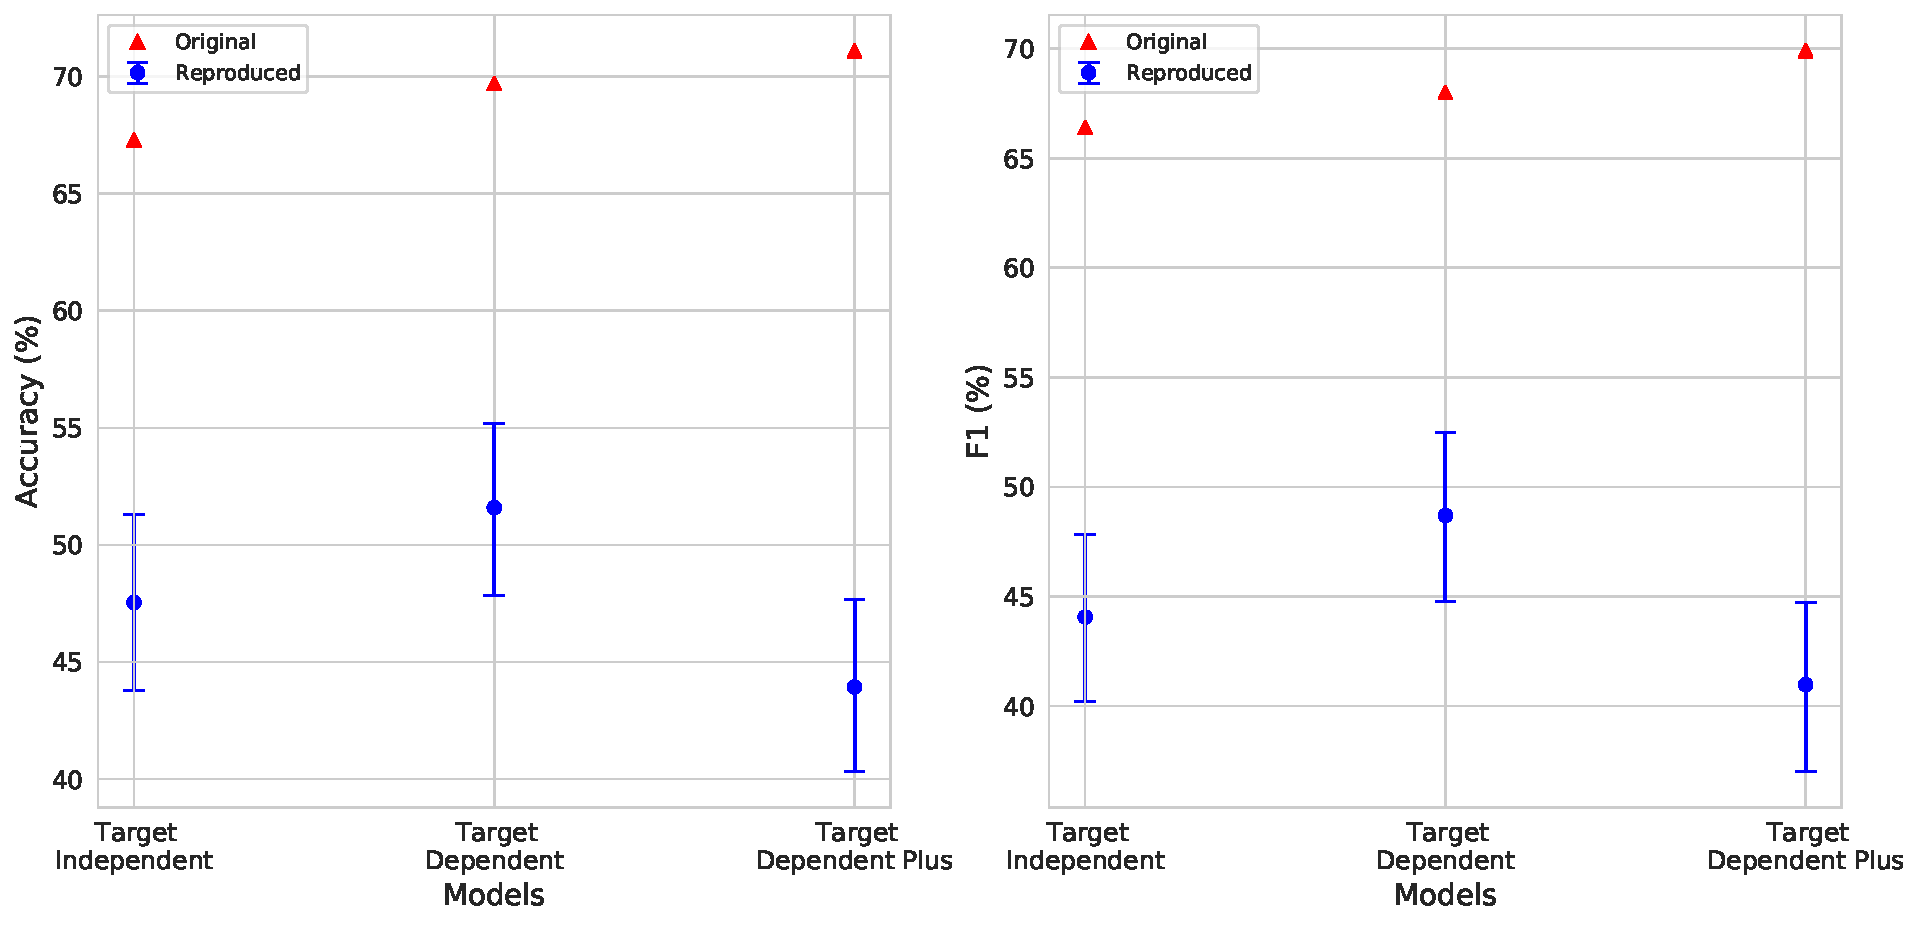
\includegraphics[scale=0.37]{images/reproducibility/vo/Target_Non_Scaled_Reproduction_Dong.pdf}
    \caption{Confidence intervals for the two tailed test for the reproduced models of \citet{vo2015target} using no scaling, on both the accuracy and macro F1 metrics. This was evaluated on the test set of \citet{dong-etal-2014-adaptive}.}
    \label{fig:repro_vo_Target_Non_Scaled_Reproduction_Dong}
\end{figure}

\subsection{Neural Pooling with Dependency Parsing}
%[I actually think he has more than that as they look at the break down of distinct sentiment. Not sure how I am going to get that metric in the theme of the thesis as this was the only paper that actually looked at the TDSA through that metric but it is a very good metric to use I think for TDSA]
To test if \citet{wang-etal-2017-tdparse} methods are reproducible, table 2 and 3 from their paper will be reproduced. These tables test their methods across two Twitter datasets, \citet{dong-etal-2014-adaptive} and their own Election Twitter dataset. To be comparable the SVM C-value is tuned using five-fold cross validation on the training data, as unlike \citet{vo2015target}, \citet{wang-etal-2017-tdparse} does not report what C-value they found to be optimal\footnote{The range of C-values \citet{wang-etal-2017-tdparse} used for tuning was not reported within the paper. However later on after the experiments within the thesis the C-value range used by \citet{wang-etal-2017-tdparse} was found through a function in their codebase: \url{https://github.com/bluemonk482/tdparse/blob/master/src/liblinear.py\#L91}.}. The range of C-values used within the tuning process is described within equation \ref{eq:repro_wang_c_values}, which is based on the exponential range suggested by \citet{hsu2003practical} with the addition of the default C-value ($1$) for linear SVMs in Scikit-learn \citep{pedregosa2011scikit}. The best found C-value for the accuracy metric, for each method, on each of the datasets can be seen in table \ref{table:repro_rep_wang_c}, these C-values will be used throughout unless otherwise stated. Additionally the same sentiment lexicons are used, but as stated earlier when using MinMax scaling the features are scaled between $0$ and $1$ rather than $-1$ and $1$. Also the same word vectors are used, which are the SSWE + w2v. As shown in figures \ref{fig:repro_wang_TDParse_Dong} and \ref{fig:repro_wang_TDParse_Election} the methods have been reproduced on both datasets.

\begin{equation}
    C=\{ 2^n | n = (i \times 2) - 17 ~for~0 < i < 10~and~i \in \Z \} \cup \{ 1 \} 
\label{eq:repro_wang_c_values}
\end{equation}

\FloatBarrier
\begin{table}[h!]
    \centering
    \begin{tabular}{|c|c|c|c|}
        \hline
         & \multicolumn{3}{c|}{Methods} \\
        \hline
        Dataset & TDParse Minus & TDParse & TDParse Plus \\
        \hline
        Dong & $2^{-5}$ & $2^{-7}$ & $2^{-7}$ \\
        \hline
        Election & $2^{-7}$ & $2^{-9}$ & $2^{-9}$ \\
        \hline
    \end{tabular}
    \caption{Best C-values for the accuracy metric for \citet{wang-etal-2017-tdparse} reproduced methods.}
    \label{table:repro_rep_wang_c}
\end{table}


\begin{figure}[!h]
    \centering
    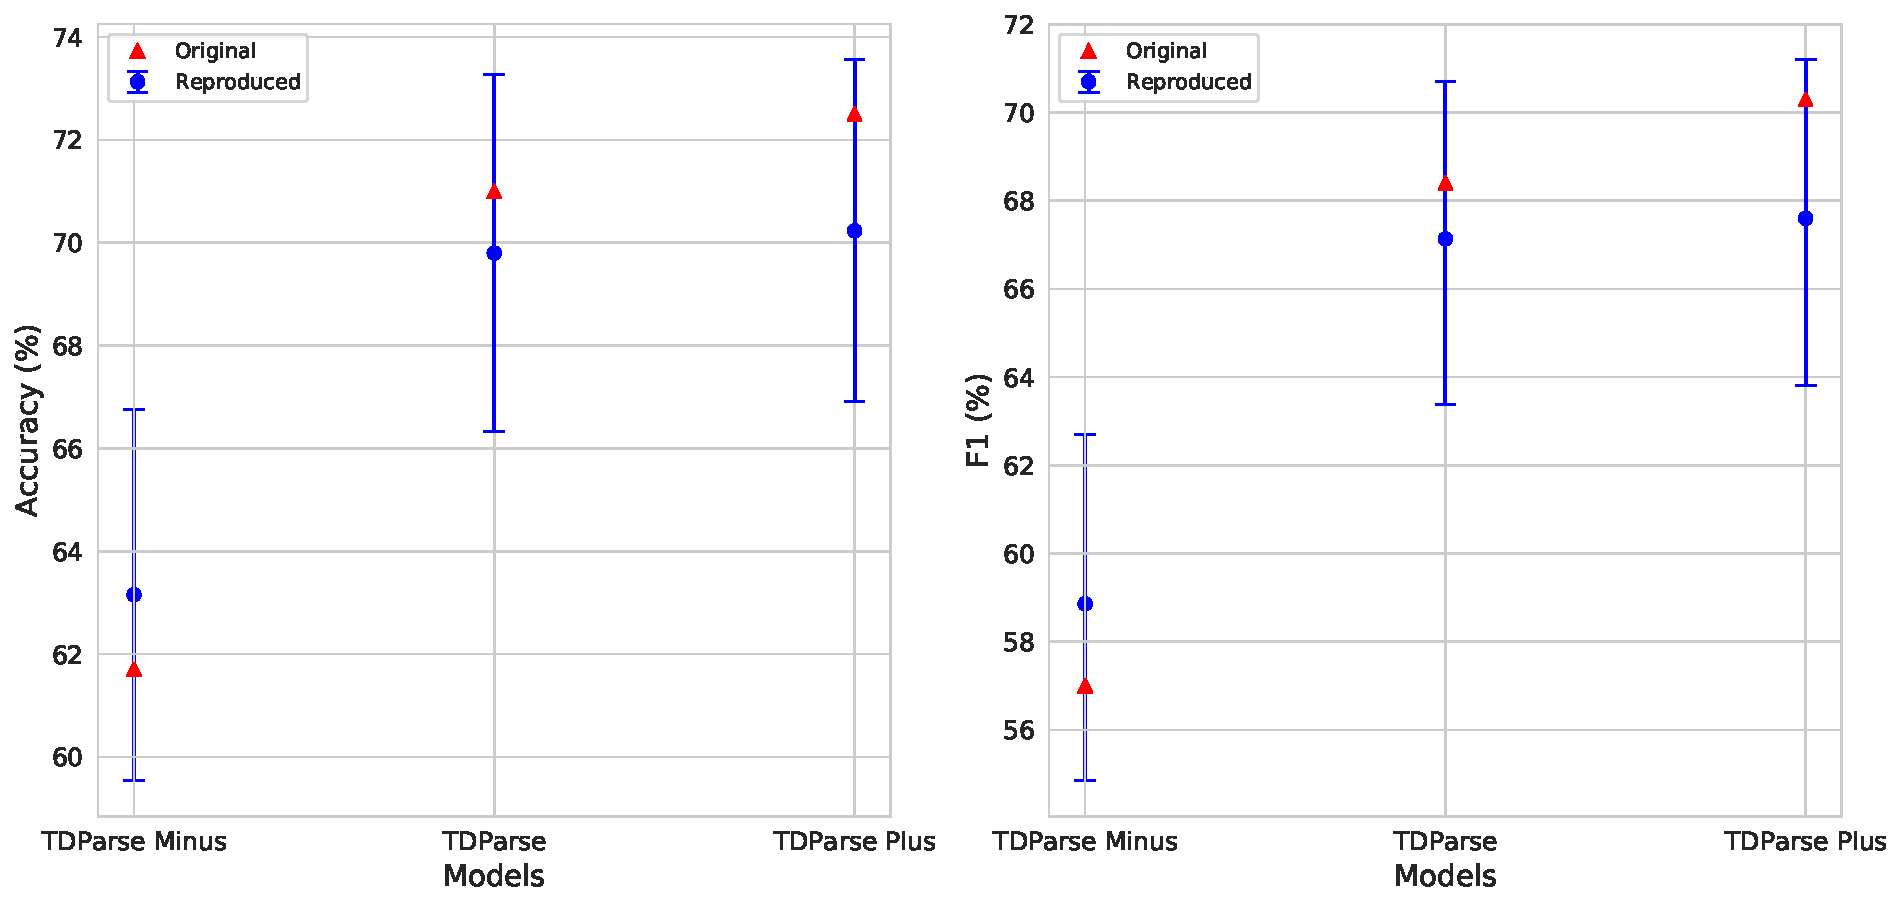
\includegraphics[scale=0.37]{images/reproducibility/wang/TDParse_Dong.pdf}
    \caption{Confidence intervals for the two tailed test on the \citet{dong-etal-2014-adaptive} test set, for the reproduced models of \citet{wang-etal-2017-tdparse}.}
    \label{fig:repro_wang_TDParse_Dong}
\end{figure}
\begin{figure}[!h]
    \centering
    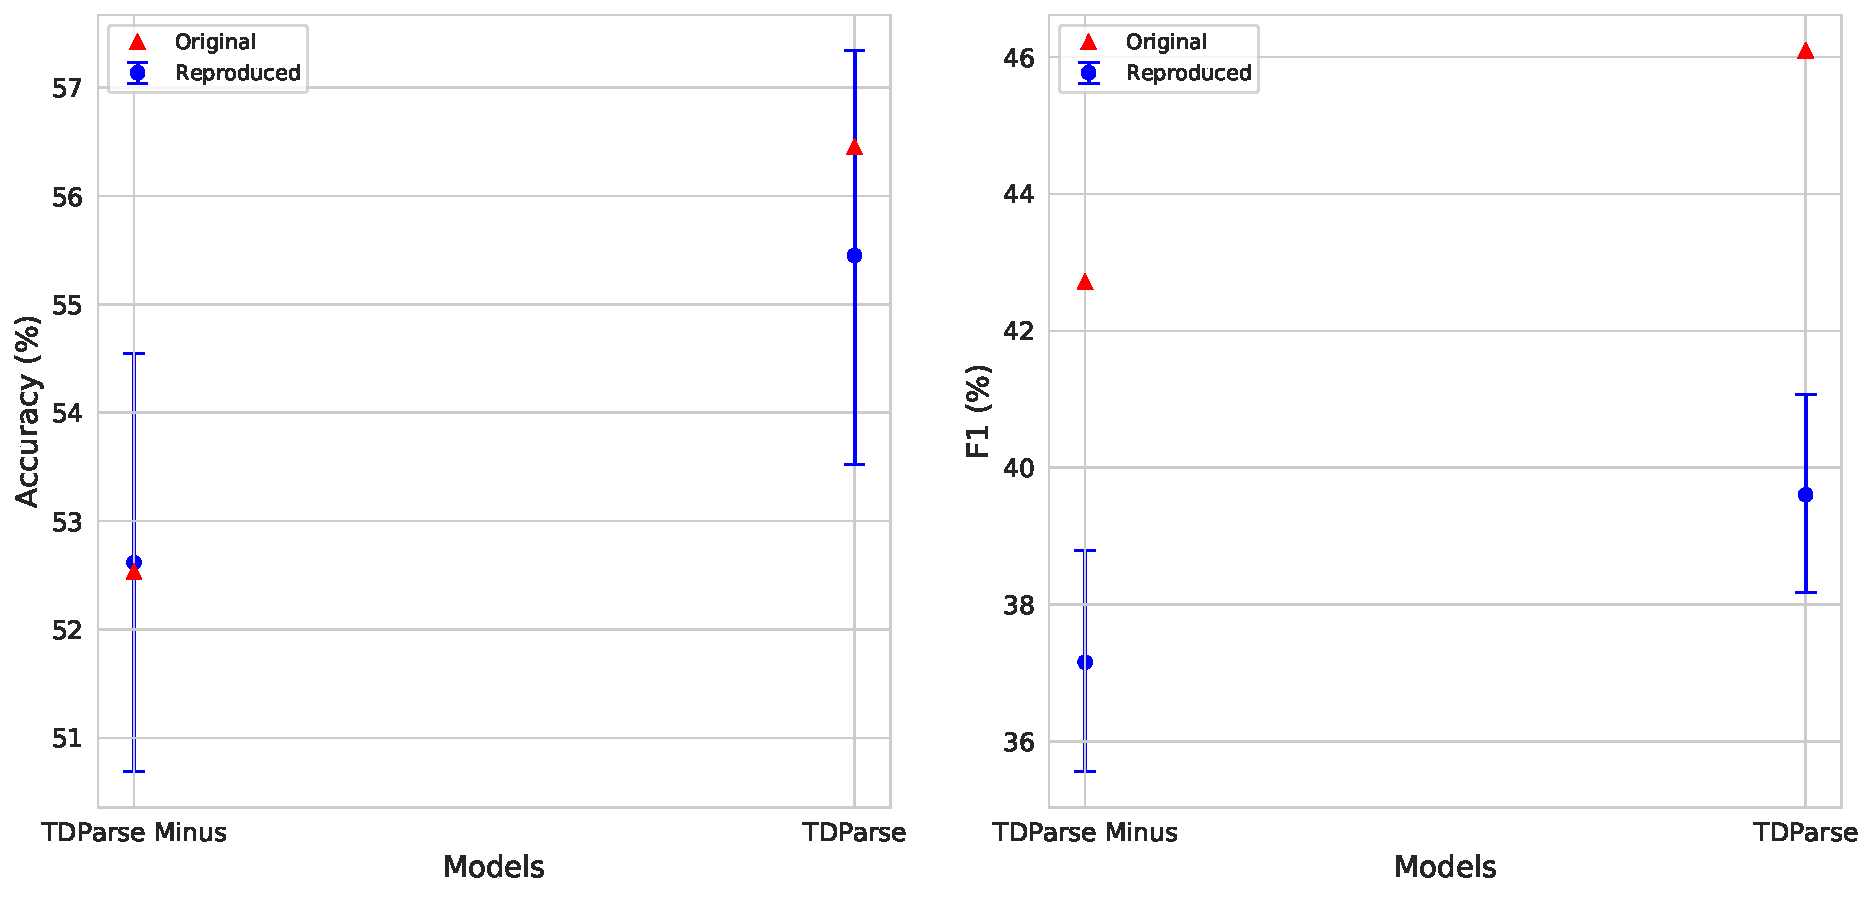
\includegraphics[scale=0.37]{images/reproducibility/wang/TDParse_Election.pdf}
    \caption{Confidence intervals for the two tailed test on the \citet{wang-etal-2017-tdparse} Election test set, for the reproduced models of \citet{wang-etal-2017-tdparse}.}
    \label{fig:repro_wang_TDParse_Election}
\end{figure}

 When using the MinMax scale range used by the original paper \citep{wang-etal-2017-tdparse} ($-1$ to $1$) the results are similar for all but the Election macro F1 scores, as shown in figures \ref{fig:repro_wang_TDParse_alt_scale_Dong} and \ref{fig:repro_wang_TDParse_alt_scale_Election}. However both the MinMax scale range used in this thesis, and the range used by \citet{wang-etal-2017-tdparse} create significantly different results to those of the original paper for the macro F1 metric on the Election dataset. Thus the same experiment is conducted, but using the C-values optimised for the macro F1 metric, where these values can be seen in table \ref{table:repro_rep_wang_c_macro_f1}\footnote{These C-values were tuned using the GloVe embeddings rather than SSWE + w2v. These embeddings were used because the C-values came from the data generated when performing the large scale C-value experiment that is performed later in this section.}. The results from this experiment can be seen in figures \ref{fig:repro_wang_TDParse_Election_macro_f1_c_values} and \ref{fig:repro_wang_TDParse_Election_alt_scaling_macro_f1_c_values} for the Election dataset\footnote{The results for the Dong dataset can be seen in appendix \ref{appendix_reproducibility_images} figures \ref{fig:repro_wang_TDParse_Dong_macro_f1_c_values} and \ref{fig:repro_wang_TDParse_Dong_alt_scaling_macro_f1_c_values}.} using the scaling range in this thesis and the scaling range of \citet{wang-etal-2017-tdparse} respectively. In both cases the macro F1 scores have increased and when using \citet{wang-etal-2017-tdparse} scaling range the original scores for macro F1 can be reproduced. Thus showing that within the original paper it is likely that they trained the methods separately with different C-values to optimise the different metric scores.  
 
 \FloatBarrier
 \begin{figure}[!h]
    \centering
    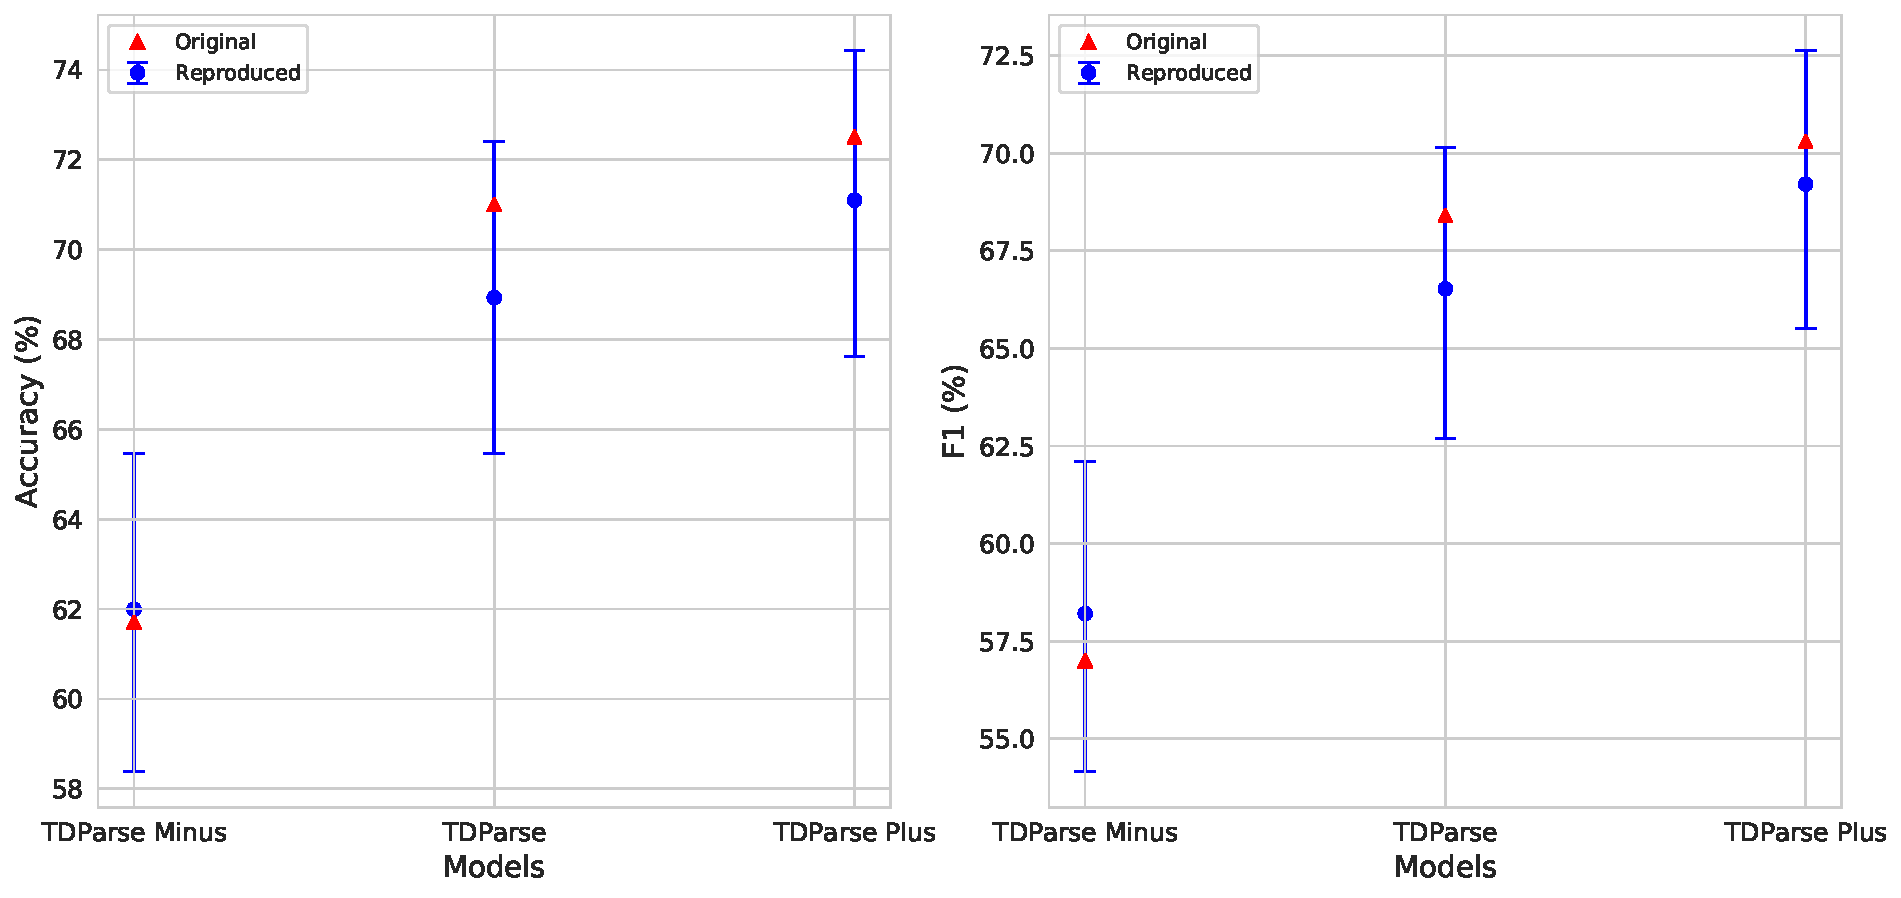
\includegraphics[scale=0.37]{images/reproducibility/wang/TDParse_alt_scale_Dong.pdf}
    \caption{Using the original MinMax scaling range of \citet{wang-etal-2017-tdparse}, the confidence intervals for the two tailed test on the \citet{dong-etal-2014-adaptive} test set.}
    \label{fig:repro_wang_TDParse_alt_scale_Dong}
\end{figure}
\begin{figure}[!h]
    \centering
    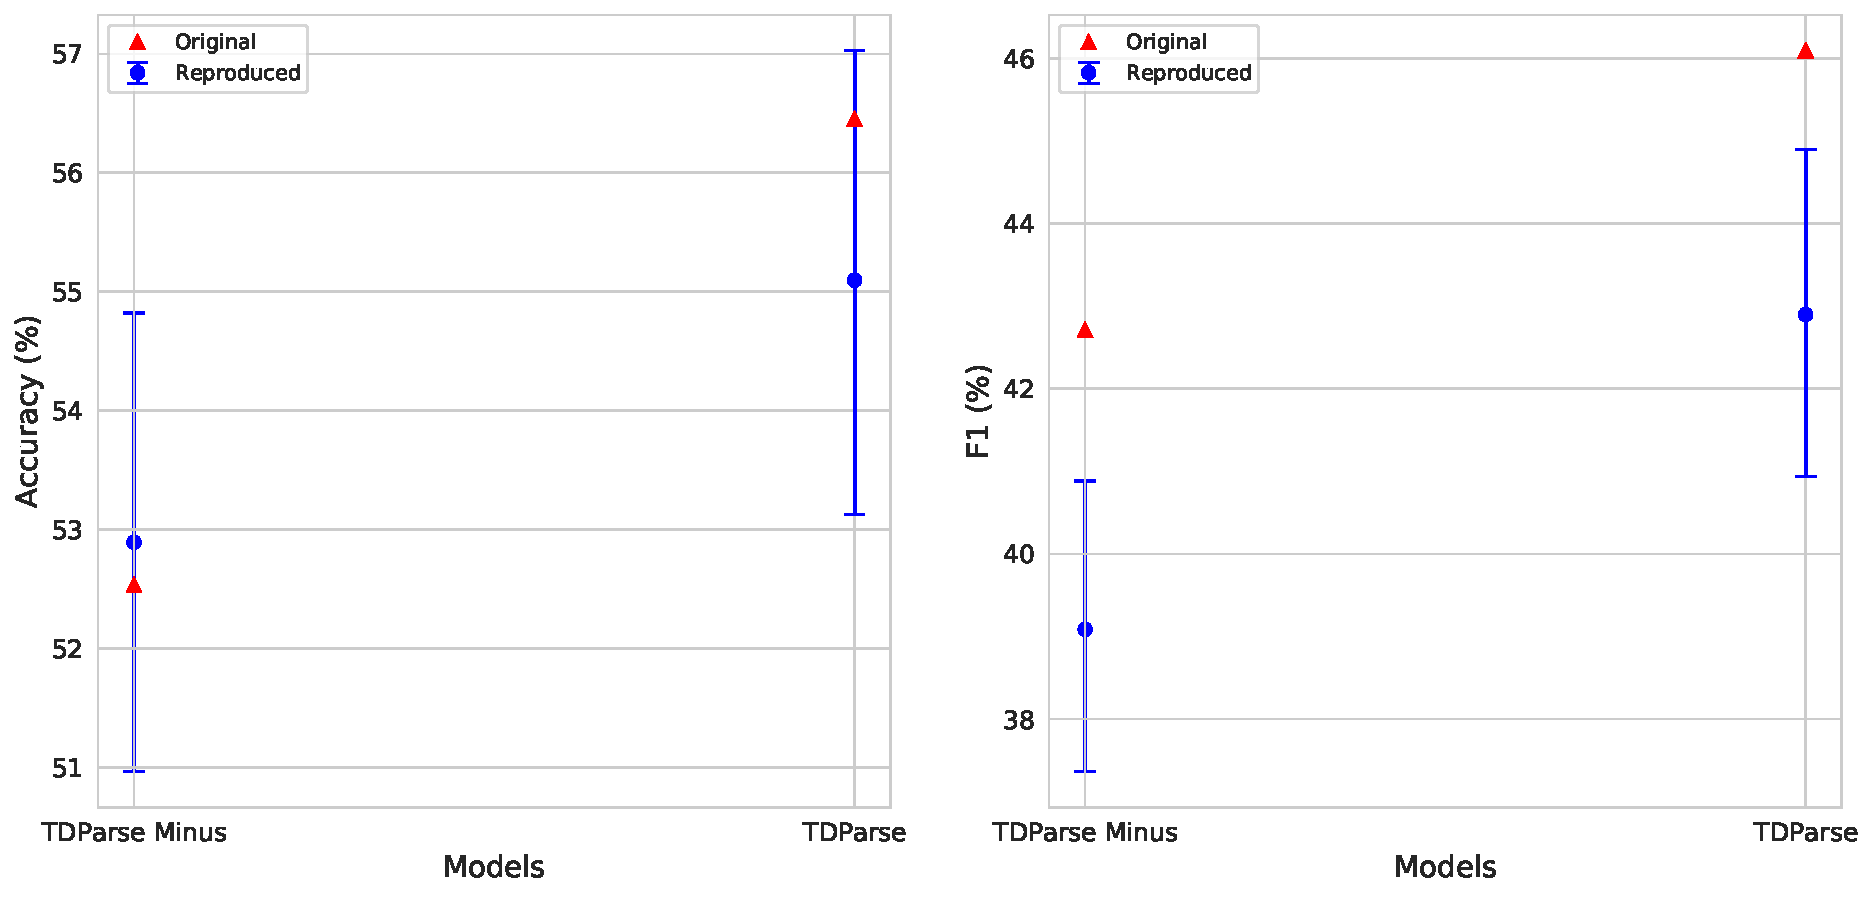
\includegraphics[scale=0.37]{images/reproducibility/wang/TDParse_alt_scale_Election.pdf}
    \caption{Using the original MinMax scaling range of \citet{wang-etal-2017-tdparse}, the confidence intervals for the two tailed test on the \citet{wang-etal-2017-tdparse} Election test set.}
    \label{fig:repro_wang_TDParse_alt_scale_Election}
\end{figure}

\begin{table}[h!]
    \centering
    \begin{tabular}{|c|c|c|c|}
        \hline
         & \multicolumn{3}{c|}{Methods} \\
        \hline
        Dataset & TDParse Minus & TDParse & TDParse Plus \\
        \hline
        Election & $2^{-3}$ & $2^{-7}$ & $2^{-7}$ \\
        \hline
    \end{tabular}
    \caption{Best C-values for the macro F1 metric for \citet{wang-etal-2017-tdparse} reproduced methods.}
    \label{table:repro_rep_wang_c_macro_f1}
\end{table}


\begin{figure}[!h]
    \centering
    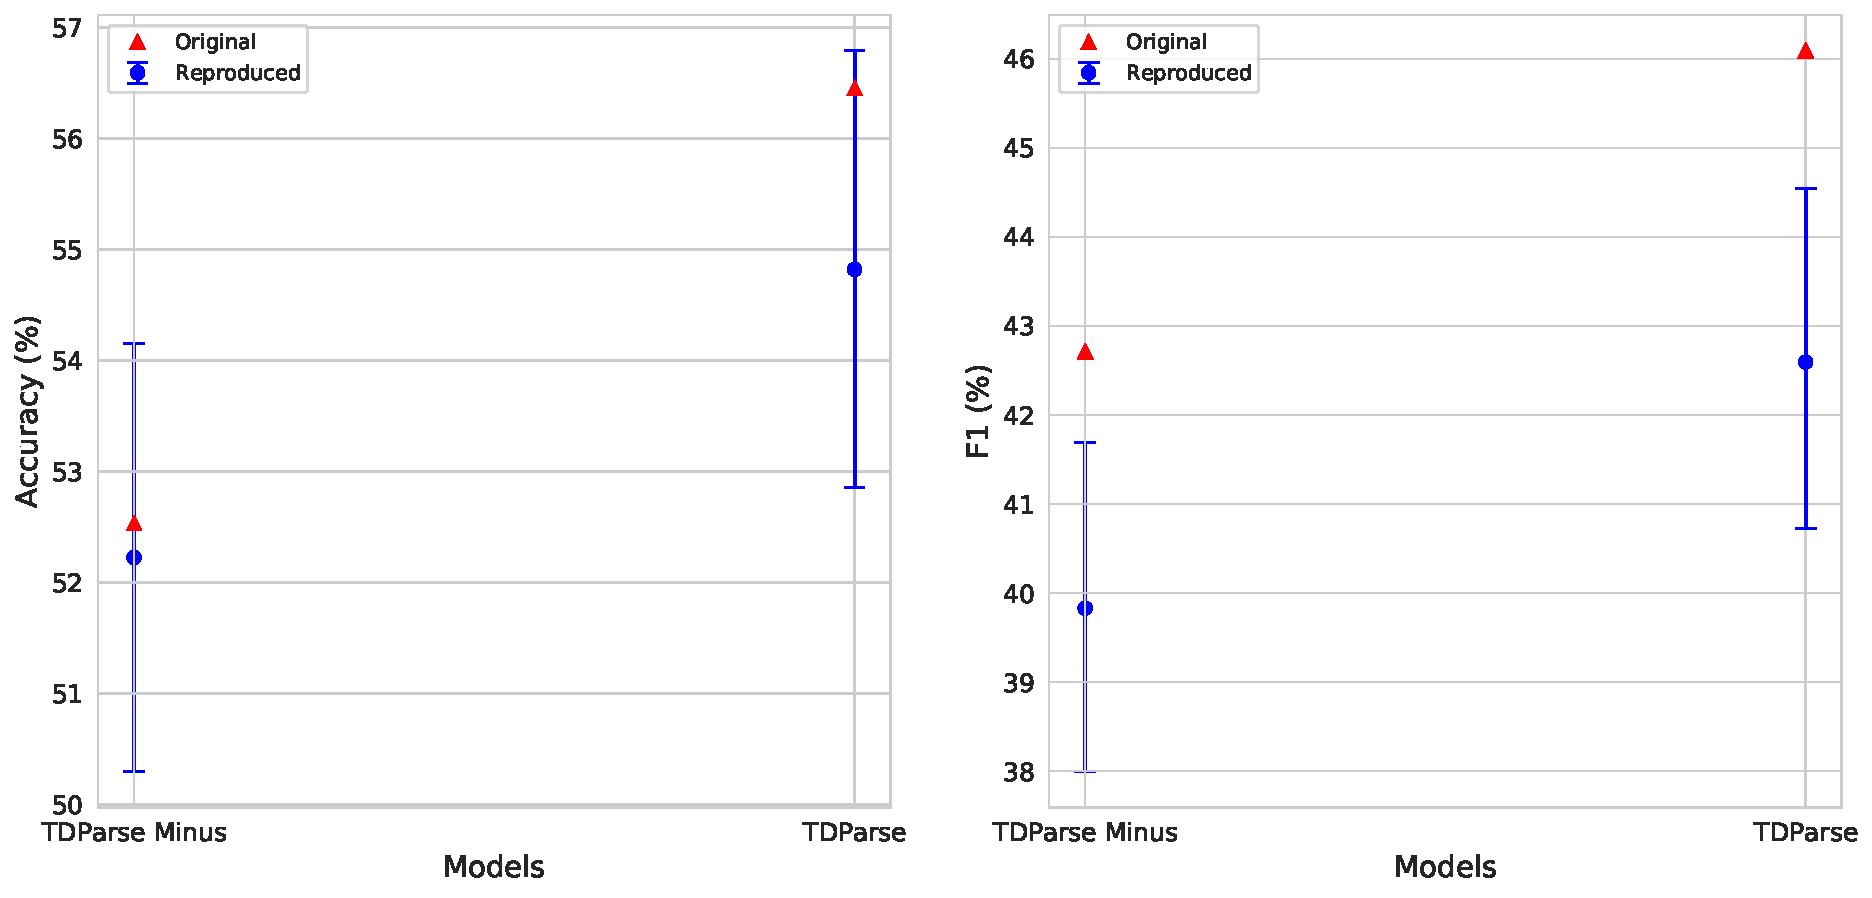
\includegraphics[scale=0.37]{images/reproducibility/wang/TDParse_F1_C_value_Election.pdf}
    \caption{Using the C-values optimised for macro F1 metric, the confidence intervals for the two tailed test on the \citet{wang-etal-2017-tdparse} Election test set.}
    \label{fig:repro_wang_TDParse_Election_macro_f1_c_values}
\end{figure}

\begin{figure}[!h]
    \centering
    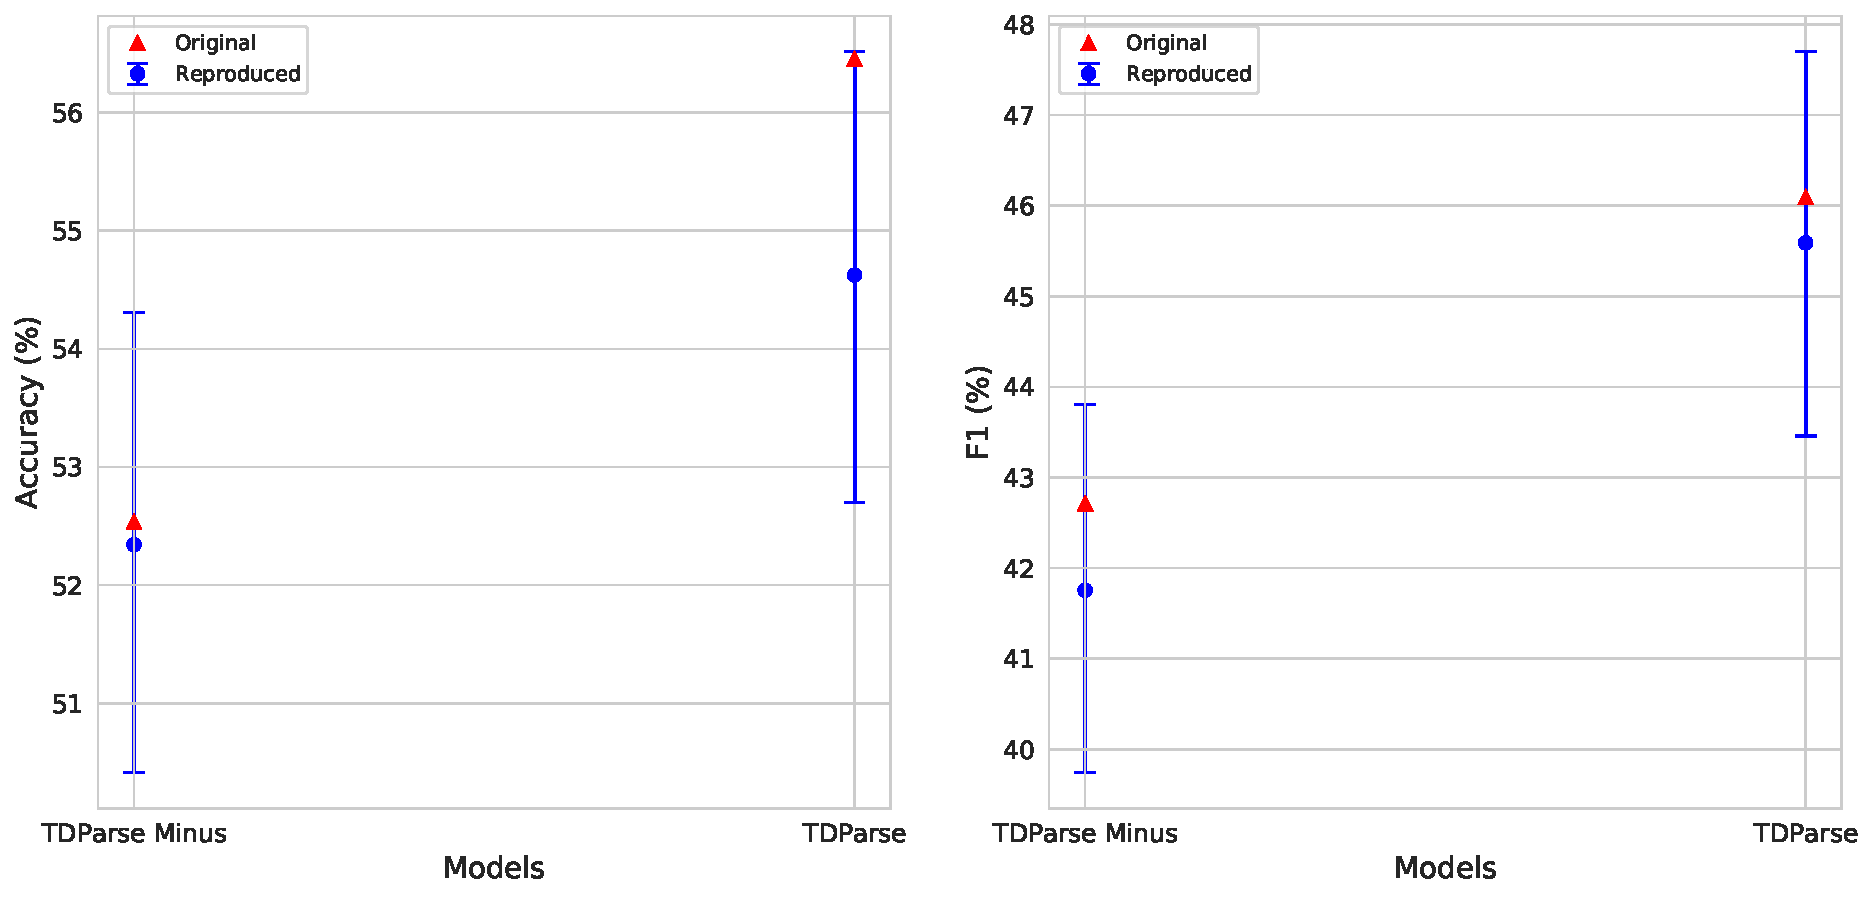
\includegraphics[scale=0.37]{images/reproducibility/wang/TDParse_F1_C_value_alt_scale_Election.pdf}
    \caption{Using the C-values optimised for macro F1 metric with the original MinMax scaling range of \citet{wang-etal-2017-tdparse}, the confidence intervals for the two tailed test on the \citet{wang-etal-2017-tdparse} Election test set.}
    \label{fig:repro_wang_TDParse_Election_alt_scaling_macro_f1_c_values}
\end{figure}

As scaling is not mentioned in the paper and only stated within the run command of the codebase, the same experiment is repeated with methods that do not scale the features. As shown in figures \ref{fig:repro_wang_TDParse_Dong_no_scale} and \ref{fig:repro_wang_TDParse_Election_no_scale} all results are significantly different and in most cases do not preserve rank order. Thus showing here again the high importance of scaling.

\begin{figure}[!h]
    \centering
    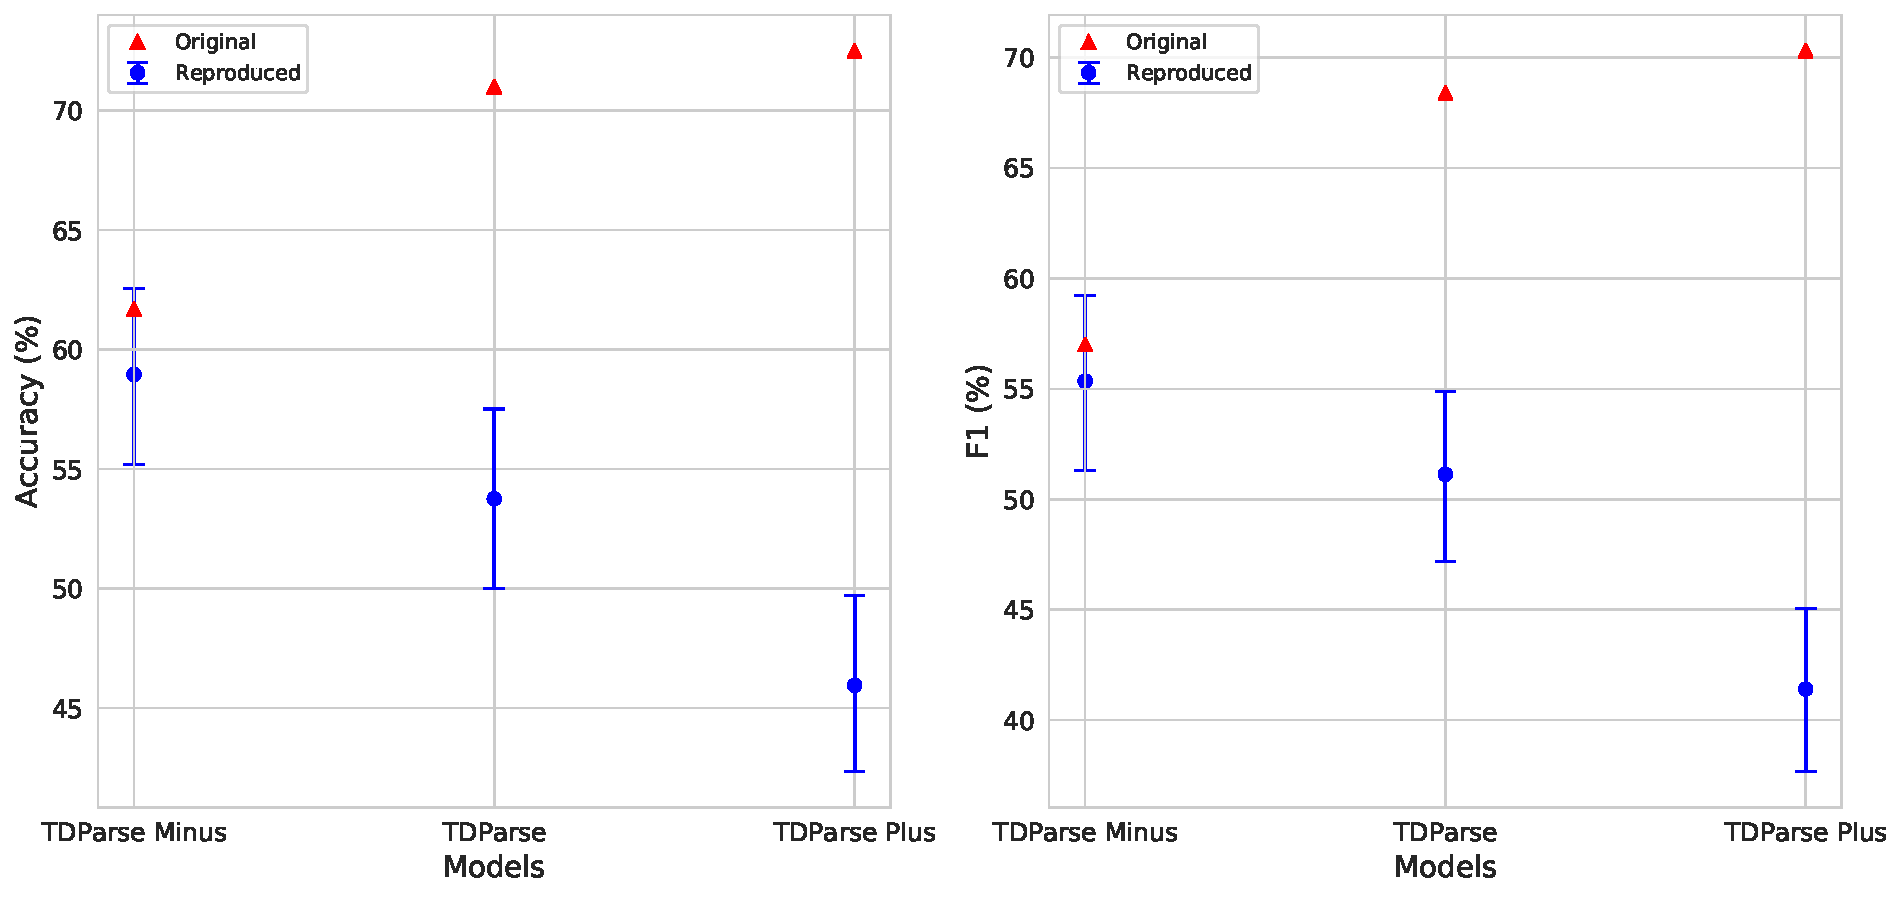
\includegraphics[scale=0.37]{images/reproducibility/wang/TDParse_no_scale_Dong.pdf}
    \caption{Using no scaling, the confidence intervals for the two tailed test on the \citet{dong-etal-2014-adaptive} test set.}
    \label{fig:repro_wang_TDParse_Dong_no_scale}
\end{figure}
\begin{figure}[!h]
    \centering
    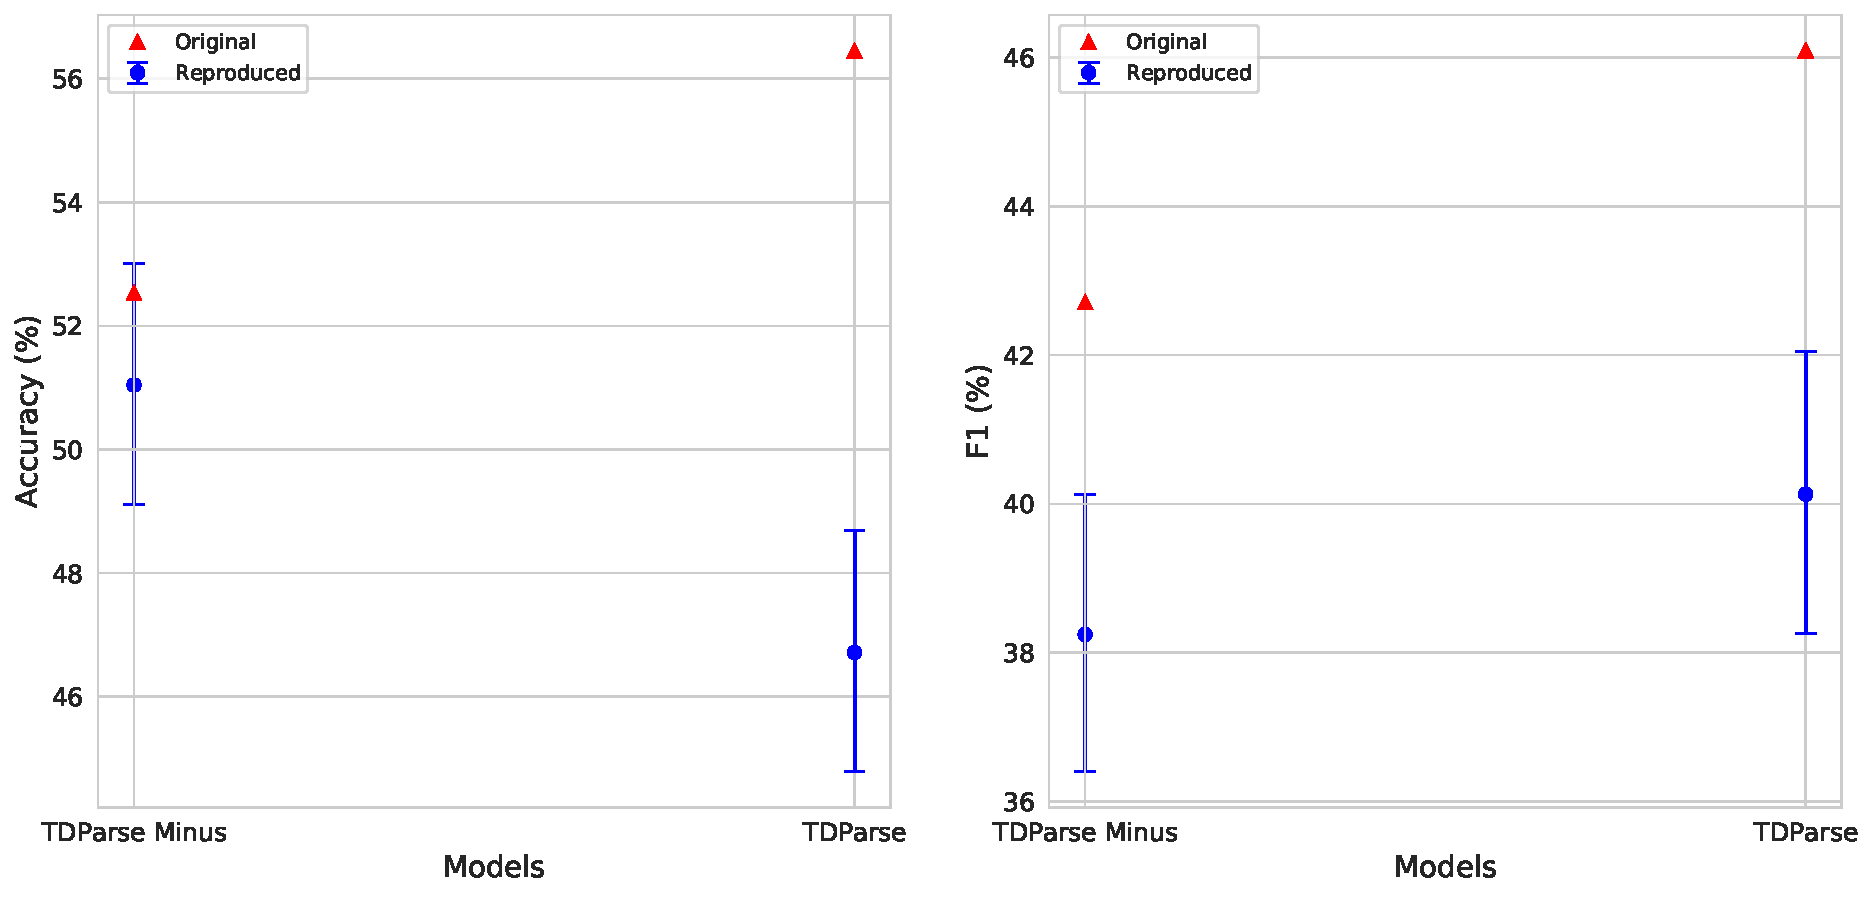
\includegraphics[scale=0.37]{images/reproducibility/wang/TDParse_no_scale_Election.pdf}
    \caption{Using no scaling, the confidence intervals for the two tailed test on the \citet{wang-etal-2017-tdparse} Election test set.}
    \label{fig:repro_wang_TDParse_Election_no_scale}
\end{figure}

The last two sets of experiments explores the importance of the C-value within the SVM that is used in the NP methods and scaling. As it has been shown that the C-value is statistically significantly important to recreate the macro F1 score within the Election dataset experiments for \citet{wang-etal-2017-tdparse} and for all NP methods scaling is statistically significant. These sets of experiments will explore how significant these two parameters are within the NP methods, whereby all of the NP methods from \citet{vo2015target} and \citet{wang-etal-2017-tdparse} will be used to make the findings more robust. Furthermore to make the findings generalisable the methods will be applied to all six datasets from table \ref{table:repro_dataset_stats}. The experiments will use five-fold cross validation on the training sets to ensure the test set is not used, and thus allow researches to use these findings without overfitting to the test sets. In all experiments the mean best performing configuration of the method for either the accuracy or macro F1 metric will be compared against all other configurations using a one sided significant test. The number of folds that the mean best configuration is significantly better than the other configurations will be corrected using Bonferroni. 

As these experiments are conducted on various different datasets, the methods will use the general non-type and non-task specific GloVe embeddings that are also the most popular in the area. For sentiment lexicon based methods the same lexicons used by \citet{wang-etal-2017-tdparse} will be used as they are a superset of the lexicons used by \citet{vo2015target} and the lexicons come from various types of data\footnote{The lexicons used originate from MPQA \citep{wilson-etal-2005-recognizing} (news data), NRC \citep{mohammad-turney-2010-emotions} (general data chosen from a dictionary based on word frequency from Google n-gram corpus \citep{brantsweb}), and \citet{hu2004mining} (review data).}. The Stanford CoreNLP tokeniser \citep{manning-etal-2014-stanford} will be used in preference to the Twitter specific tokeniser; Twokenizer \citep{gimpel-etal-2011-part} to avoid type specific tools. For \citet{wang-etal-2017-tdparse} methods that require a dependency parser the TweeboParser \citep{kong-etal-2014-dependency} will be used on all datasets but the Laptop and Restaurant datasets, whereby the Stanford CoreNLP dependency parser will be used. This decision was made before realising the importance of a dependency parser creating multiple roots for \citet{wang-etal-2017-tdparse} methods and Stanford's parser does not create multiple roots. Thus in effect Stanford's parser will create a context that is almost identical to the whole text context\footnote{The reason it is not the same is due to the context not including the target word(s). Also Stanford's parser requires the text to go through their sentence splitter first, which in some cases does cause the text to be split up.}. Stanford's parser was chosen due to the Laptop and Restaurant datasets coming from a different type of data (review rather than social media) and thus is believed to require a more type relevant parser, such as the Stanford parser. 

The SVM C-value is part of the L2-regularised L2-loss function of the linear SVM which can be seen in equation \ref{eq:repro_svm} (taken from equation 1 in \citep{fan2008liblinear}). The L2-regularisation in the equation is $\frac{1}{2}w^Tw$ and the rest is the L2-loss. As can be seen the C-value determines the amount of weight the L2-loss has on the overall loss function. Thus if the C-value is large the effect of the regularisation is small, which would more likely cause the model to overfit to the training data.

\begin{equation}
    \frac{1}{2}w^{T}w + C\sum_{i=1}^{l}(\max(0, 1 - y_{i}w^{T}x_i))^2
    \label{eq:repro_svm}
\end{equation}

The C-values that will be tested here are the same as those evaluated for the reproduction of \citet{wang-etal-2017-tdparse}, shown in equation \ref{eq:repro_wang_c_values}. Figures \ref{fig:repro_parameters_c_values_accuracy} and \ref{fig:repro_parameters_c_values_macro_f1} show the mean best C-values for each method on each dataset for the accuracy and macro F1 metric respectively. In both cases it can be seen that all methods are significantly sensitive to the choice in C-value no matter the dataset. In most cases and more so for the accuracy metric the default C-value from scikit-learn \citep{pedregosa2011scikit} ($1$) is significantly worse than the mean best. It would be assumed that datasets that are small like YouTuBean would prefer a small C-value to stop the methods from overfitting, but that does not seem to be the case. Rather it would appear that for both the accuracy and macro F1 score each have their own preferable band of C-values. For accuracy, generally $7.81e^{-3}$ performs well on all methods and datasets, whereas for macro F1 it is dataset and method specific. Furthermore a C-value that performs best for accuracy could be significantly worse than the best C-value for macro F1, of which this happens the most on the Election dataset. For the mean best scores produced by these C-values for all methods on all datasets see figures \ref{fig:repro_parameters_c_accuracy_plot} and \ref{fig:repro_parameters_c_macro_f1_plot} in appendix \ref{appendix_reproducibility_images}.

\begin{figure}[!h]
    \centering
    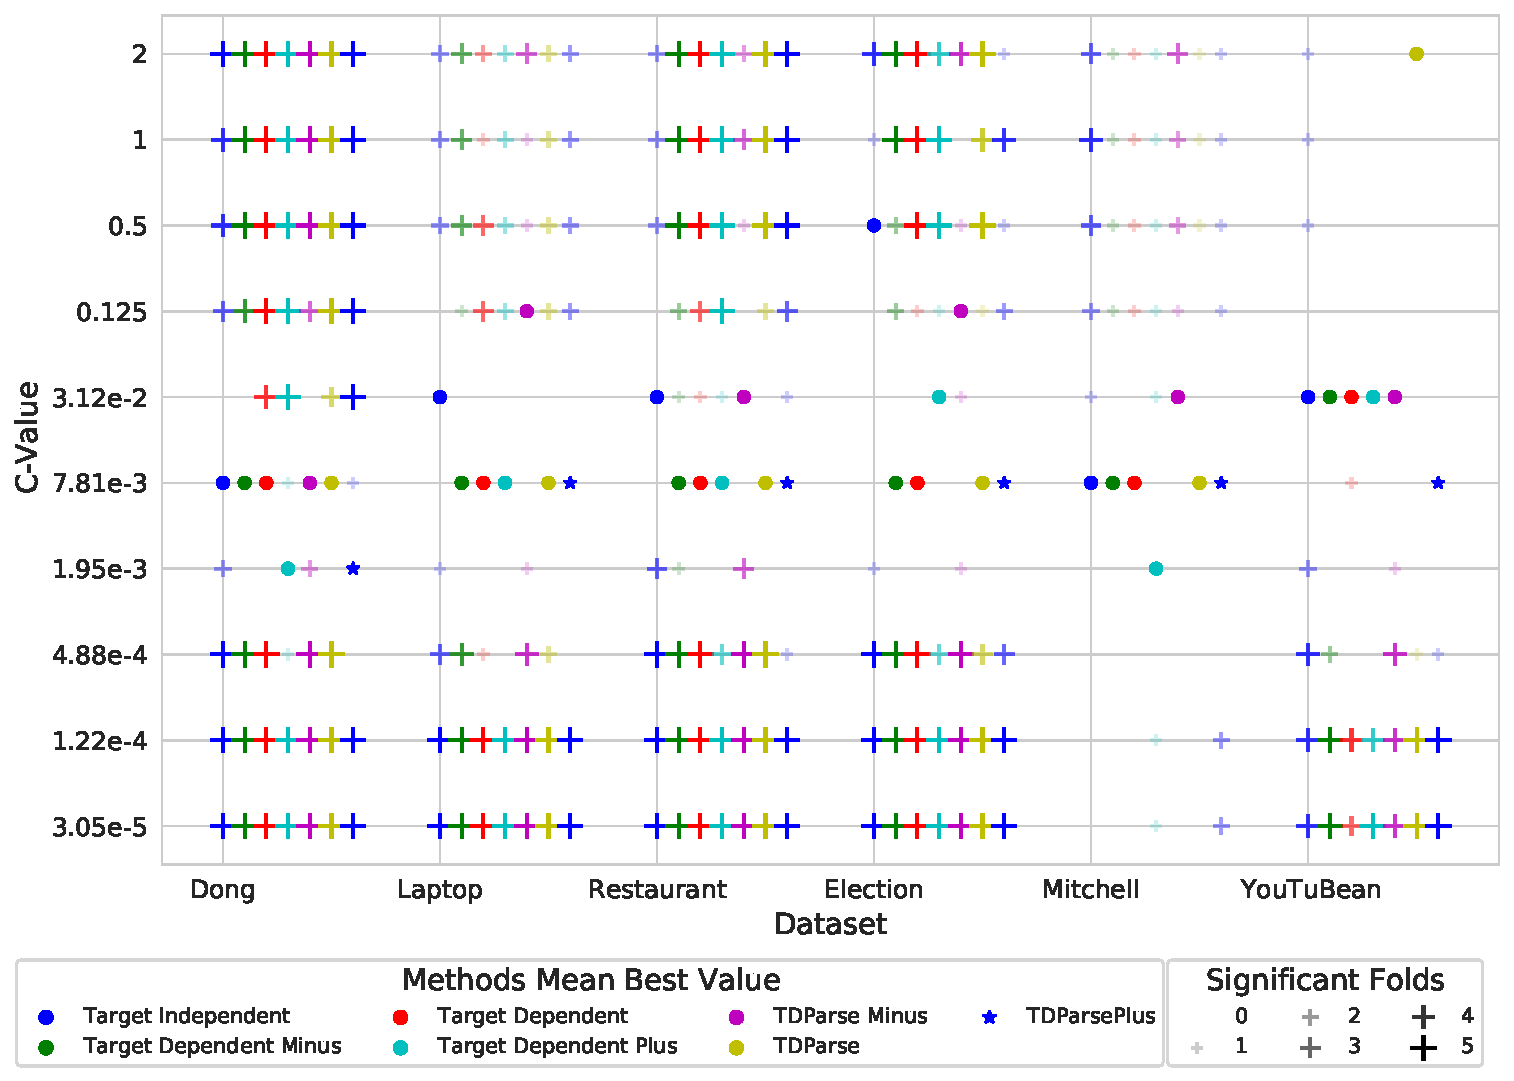
\includegraphics[scale=0.47]{images/reproducibility/Parameters/C_Value/C_Sig_Plot_Accuracy.pdf}
    \caption{For the accuracy metric the mean best C-value for each method and dataset represented by dots and star. The size of the cross indicates the number of folds the mean best C-value is significantly better than the other C-values for the given method and dataset.}
    \label{fig:repro_parameters_c_values_accuracy}
\end{figure}
\begin{figure}[!h]
    \centering
    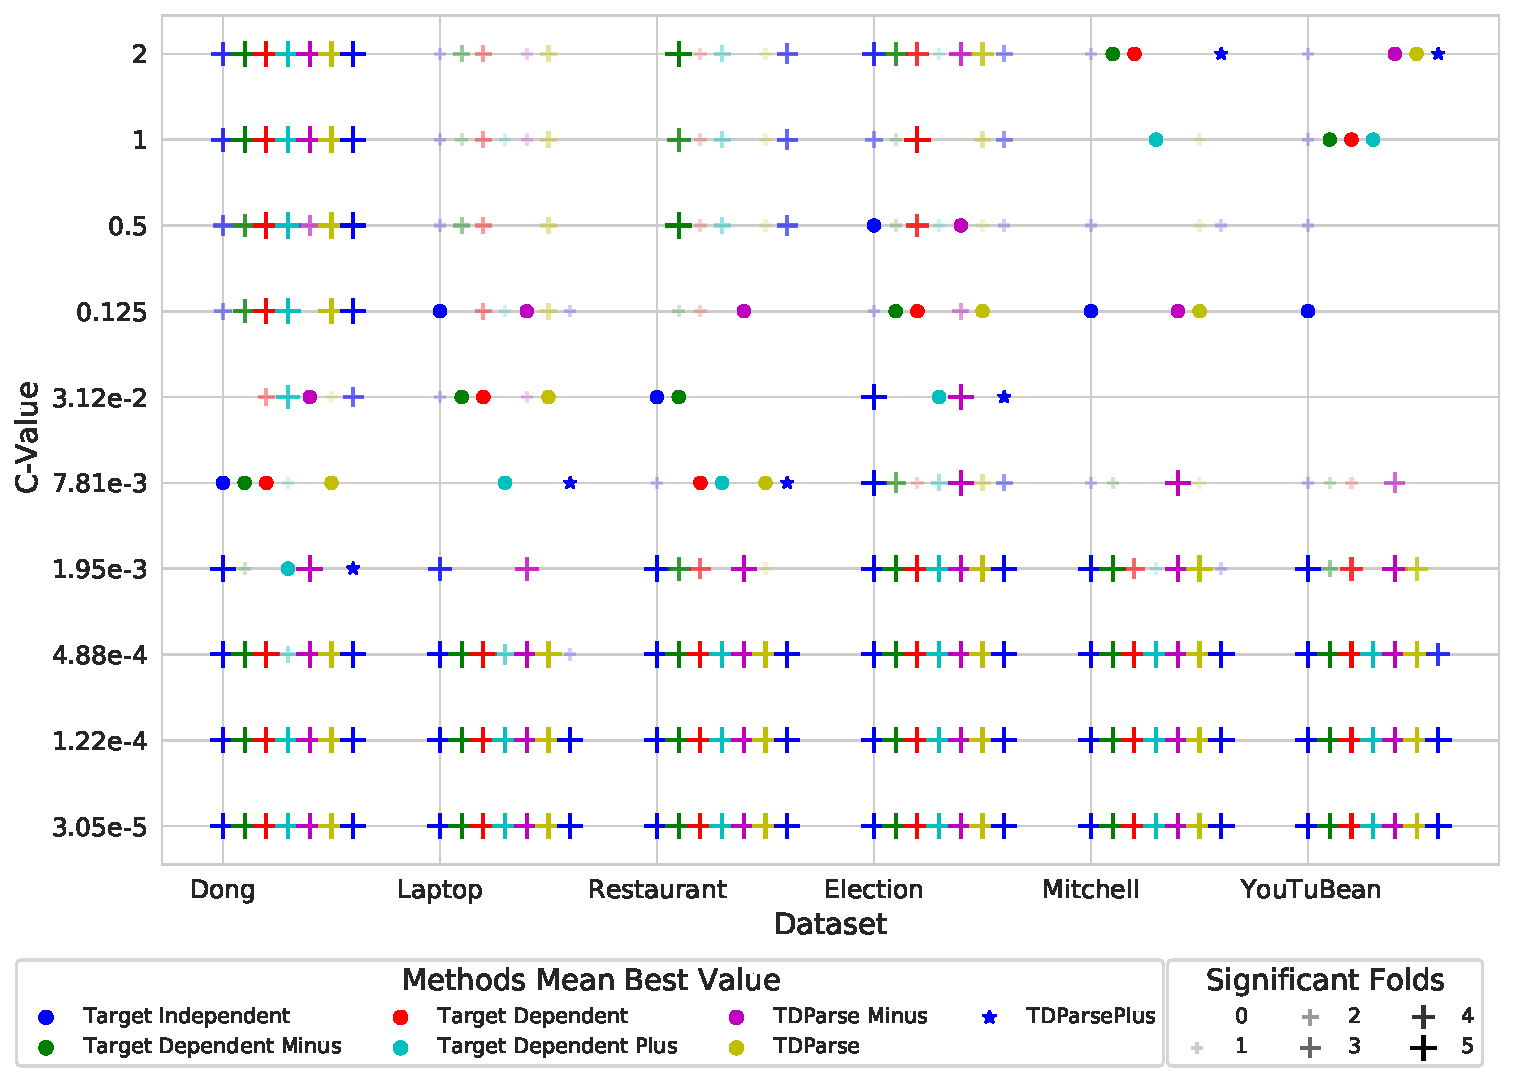
\includegraphics[scale=0.47]{images/reproducibility/Parameters/C_Value/C_Sig_Plot_F1.pdf}
    \caption{For the macro F1 metric the mean best C-value for each method and dataset represented by dots and star. The size of the cross indicates the number of folds the mean best C-value is significantly better than the other C-values for the given method and dataset.}
    \label{fig:repro_parameters_c_values_macro_f1}
\end{figure}
\clearpage

MinMax scaling with the scale range of $0$ to $1$, rather than \citet{wang-etal-2017-tdparse} $-1$ to $1$, will be compared to not scaling. When performing these experiments the optimal C-value for each method on each dataset for the accuracy metric is used, which was found from the last experiment. The results can be seen in figures \ref{fig:repro_parameters_c_values_accuracy} and \ref{fig:repro_parameters_c_values_macro_f1}. It can be clearly seen in all cases for the accuracy metric and the majority for the macro F1 metric that scaling is statistically significant no matter the method nor dataset, with the caveat of Mitchell for the macro F1 metric. For the mean best scores produced by these scaling experiments for all methods on all datasets see figures \ref{fig:repro_parameters_scaling_accuracy_plot} and \ref{fig:repro_parameters_scaling_macro_f1_plot} in appendix \ref{appendix_reproducibility_images}.

\begin{figure}[!h]
    \centering
    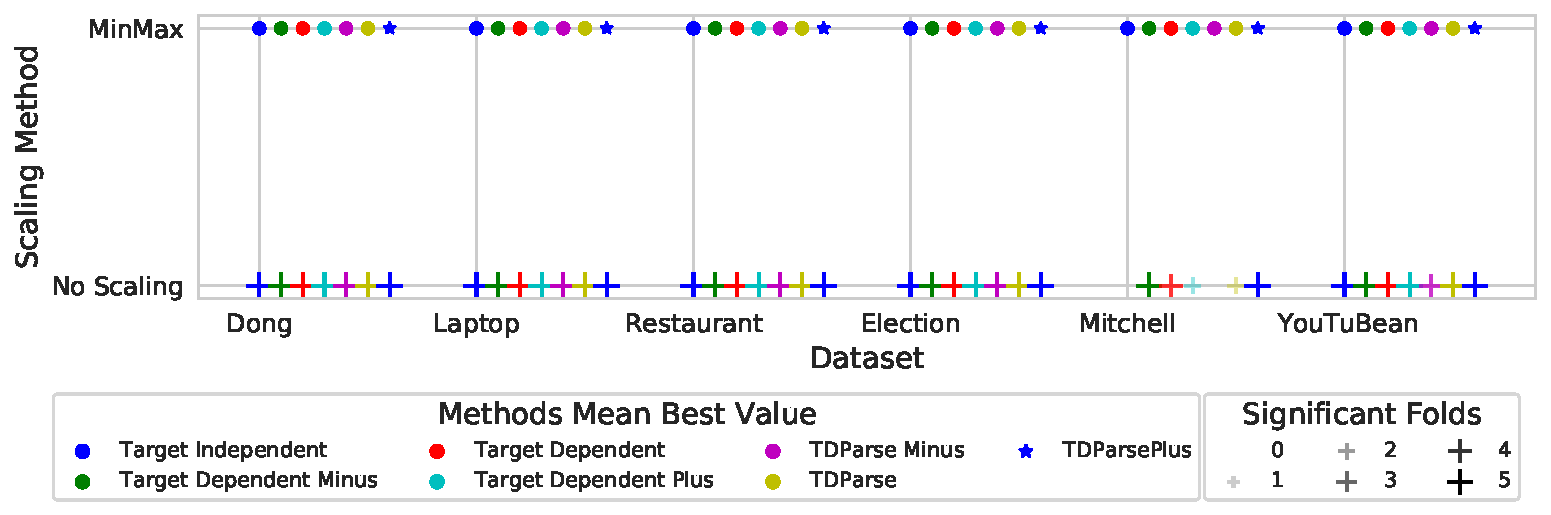
\includegraphics[scale=0.47]{images/reproducibility/Parameters/Scaling/Scaling_Sig_Plot_Accuracy.pdf}
    \caption{For the accuracy metric the mean best scaling method for each method and dataset represented by dots and star. The size of the cross indicates the number of folds the mean best scaling method is significantly better than the other scaling method for the given method and dataset.}
    \label{fig:repro_parameters_scaling_accuracy}
\end{figure}
\begin{figure}[!h]
    \centering
    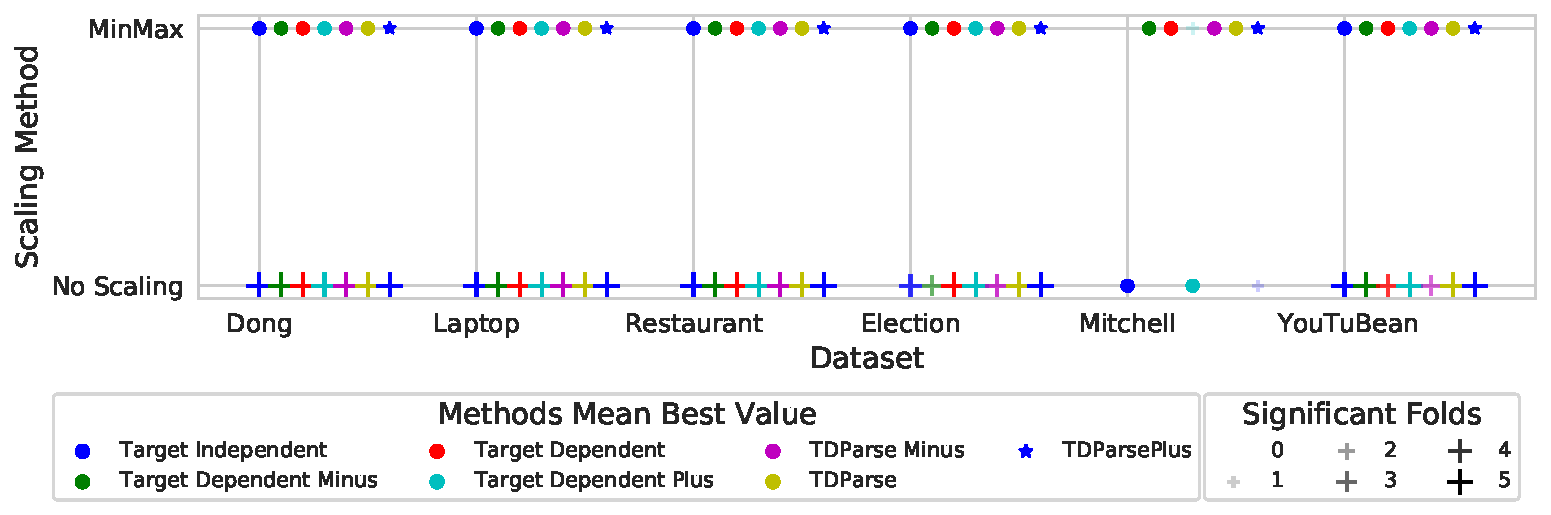
\includegraphics[scale=0.47]{images/reproducibility/Parameters/Scaling/Scaling_Sig_Plot_F1.pdf}
    \caption{For the macro F1 metric the mean best scaling method for each method and dataset represented by dots and star. The size of the cross indicates the number of folds the mean best scaling method is significantly better than the other scaling method for the given method and dataset.}
    \label{fig:repro_parameters_scaling_macro_f1}
\end{figure}


% Furthermore \citet{reimers-gurevych-2017-reporting} found that the same NN based sequence labelling method can produce statistically significantly different results based on the random seed the method was initialised with.

\subsection{LSTM}
\label{section:repro_lstm}

It has been found that in the previous work it is difficult to either reproduce \citep{tay2018learning} or replicate \citep{chen-etal-2017-recurrent} \citet{tang-etal-2016-effective} LSTM based methods, most specifically the TDLSTM version, as shown by table \ref{table:repro_tang_authors_differences}\footnote{The original \citet{tang-etal-2016-effective} methods as stated in this section were never originally evaluated on the Laptop or Restaurant datasets. However the original authors within another paper \citep{tang-etal-2016-aspect} evaluated the TDLSTM method they created on the Laptop and Restaurant datasets and that is what is meant by original authors within the table.}. Based on these findings the methods in \citet{tang-etal-2016-effective} are reproduced. The reproduced methods are evaluated on \citet{dong-etal-2014-adaptive} Twitter dataset and use the same GloVe Twitter 100 dimension embeddings \citep{pennington-etal-2014-glove}. All methods used Stochastic Gradient Descent (SGD) with a learning rate of $0.01$, a cross entropy loss, and the hidden dimension of all LSTMs equal to the dimension of the embedding being used. However the paper did not state the number of epochs the method was trained for thus early stopping is used keeping track of the loss value with a patience of $10$. As early stopping requires a validation set, the training set is split $80\%$ training and $20\%$ validation. The paper also mentioned that they ``set the clipping threshold of softmax layer as 200'' \citep{tang-etal-2016-effective} as this did not make sense, this was not used. Lastly all weights were initialised using $\mathcal{U}(-\sqrt{k}, \sqrt{k})$\footnote{This is the default initialisation within PyTorch \citep{NEURIPS2019_9015} and AllenNLP \citep{gardner-etal-2018-allennlp}.} where $k = \frac{1}{\text{embedding dimension}}$. The original initialisation from \citet{tang-etal-2016-effective}, $\mathcal{U}(-0.003, 0.003)$, always overfitted to the dominant class\footnote{Which is neutral for \citet{dong-etal-2014-adaptive} as shown by table \ref{table:repro_dataset_sent_dist}.} when used in the reproduced methods, hence the difference in the initialisation distributions. The tokeniser used was Spacy, as the original tokeniser that was used was not stated in the paper\footnote{To note in the original paper \citep{moore-rayson-2018-bringing} that this chapter is based on the results for \citet{tang-etal-2016-effective} did use the original weight initialisation of \citet{tang-etal-2016-effective} ($\mathcal{U}(-0.003, 0.003)$) and could still reproduce the results. The main implementation difference between \citet{moore-rayson-2018-bringing} and this chapter is that here PyTorch \citep{NEURIPS2019_9015} and AllenNLP \citep{gardner-etal-2018-allennlp} is used rather than Keras \citep{chollet2015keras} and also the Spacy tokeniser is used rather than Twokenizer \cite{gimpel-etal-2011-part} tokeniser. It is unknown why the original weight initialisation did not work within the code implementation of this chapter, it is believed it could be due to subtle differences between Keras and PyTorch.}. 




\begin{table}[!h]
    \centering
    \begin{tabular}{|c|c|c|}
        \hline
        Authors & Restaurant & Laptop\\
        \hline
        \posbox{\citet{tang-etal-2016-aspect}} & 75.63 & 68.13 \\
        \hline
        \negbox{\citet{chen-etal-2017-recurrent}} & 78.00 & 71.83 \\
        \hline
        \neubox{\citet{tay2018learning}} & 69.73 & 62.38 \\
        \hline
        \multicolumn{3}{|c|}{\centering \cbox{lightblue} Original authors \quad \cbox{lightred} Replicated \quad \cbox{lightgrey} Reproduced} \\
        \hline
    \end{tabular}
    \caption{Accuracy of the TDLSTM method by the different authors on the Restaurant and Laptop datasets.}
    \label{table:repro_tang_authors_differences}
\end{table}

The results from the experiment can be seen in table \ref{table:tang_twitter_100_results} and figure \ref{fig:repro_tang_LSTM_DIST_ACC_F1} whereby each reproduced method has been ran $20$ times. Running each method $20$ times using different random seeds allows the methods to take into account the random initialisation problem \citep{reimers-gurevych-2017-reporting}. It can be seen that if the maximum score is used the original and reproduced results are quite close, and statistically similar as shown by figure \ref{fig:repro_tang_LSTM_ACC_F1}\footnote{The best run for accuracy is not always the same best run for macro F1. Therefore we only use the best run for each method based on the metric being evaluated.}. Furthermore based on the maximum score the rank of the methods are the same as the original, thus the methods have been reproduced successfully. However the difference between the maximum result and the minimum can be quite large, especially for the macro F1 metric.

\begin{table}[!h]
    \centering
    \begin{tabular}{|c|c|c|c|c|c|}
\hline
Metric &    Method    &   Max &   Mean &   Min & Original \\
\hline
Accuracy & LSTM &  64.31 &  62.93 &  61.42 & 66.5 \\
& TDLSTM &  69.36 &  \textbf{67.23} &  \textbf{65.46} & 70.8 \\
& TCLSTM &  \textbf{70.23} &  66.74 &  64.74 & 71.5 \\
\hline
macro F1 & LSTM &  61.93 &  58.59 &  54.43 & 64.7 \\
& TDLSTM &  66.58 &  \textbf{63.86} &  59.94 & 69.0 \\
& TCLSTM &  \textbf{67.61} &  63.26 &  \textbf{60.29} & 69.5 \\
\hline
\end{tabular}
    \caption{The max, mean, and minimum (min) scores from each reproduced method over $20$ runs. The last column are the original scores from the \citet{tang-etal-2016-effective} paper. The \textbf{bold} scores represent the best performing score between the methods for each metric, max, mean, and minimum.}
    \label{table:tang_twitter_100_results}
\end{table}

\begin{figure}[!h]
    \centering
    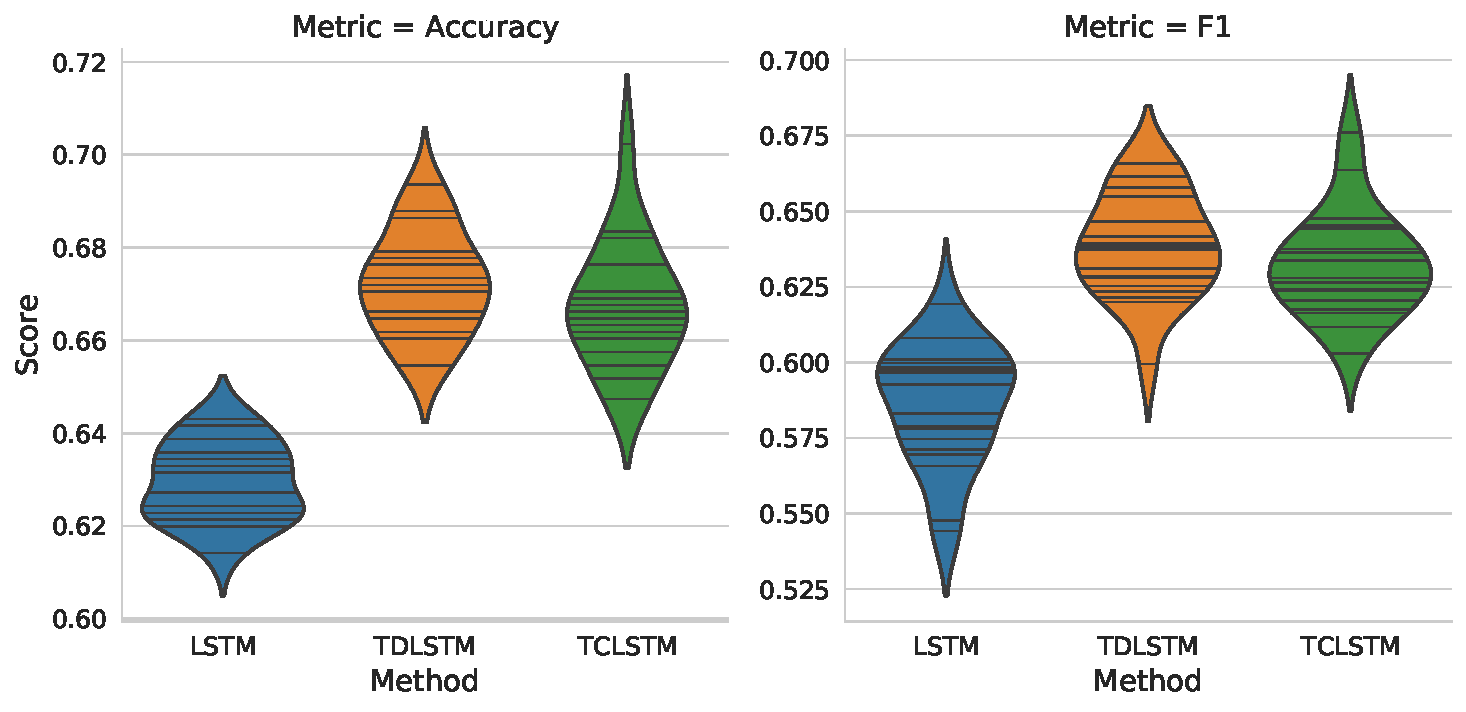
\includegraphics[scale=0.4]{images/reproducibility/tang/LSTM_DIST_ACC_F1.pdf}
    \caption{The distribution of scores for each of the $20$ runs for each reproduced method. Whereby each horizontal line in the distribution represent the result of one run for the reproduced method.}
    \label{fig:repro_tang_LSTM_DIST_ACC_F1}
\end{figure}

\begin{figure}[!h]
    \centering
    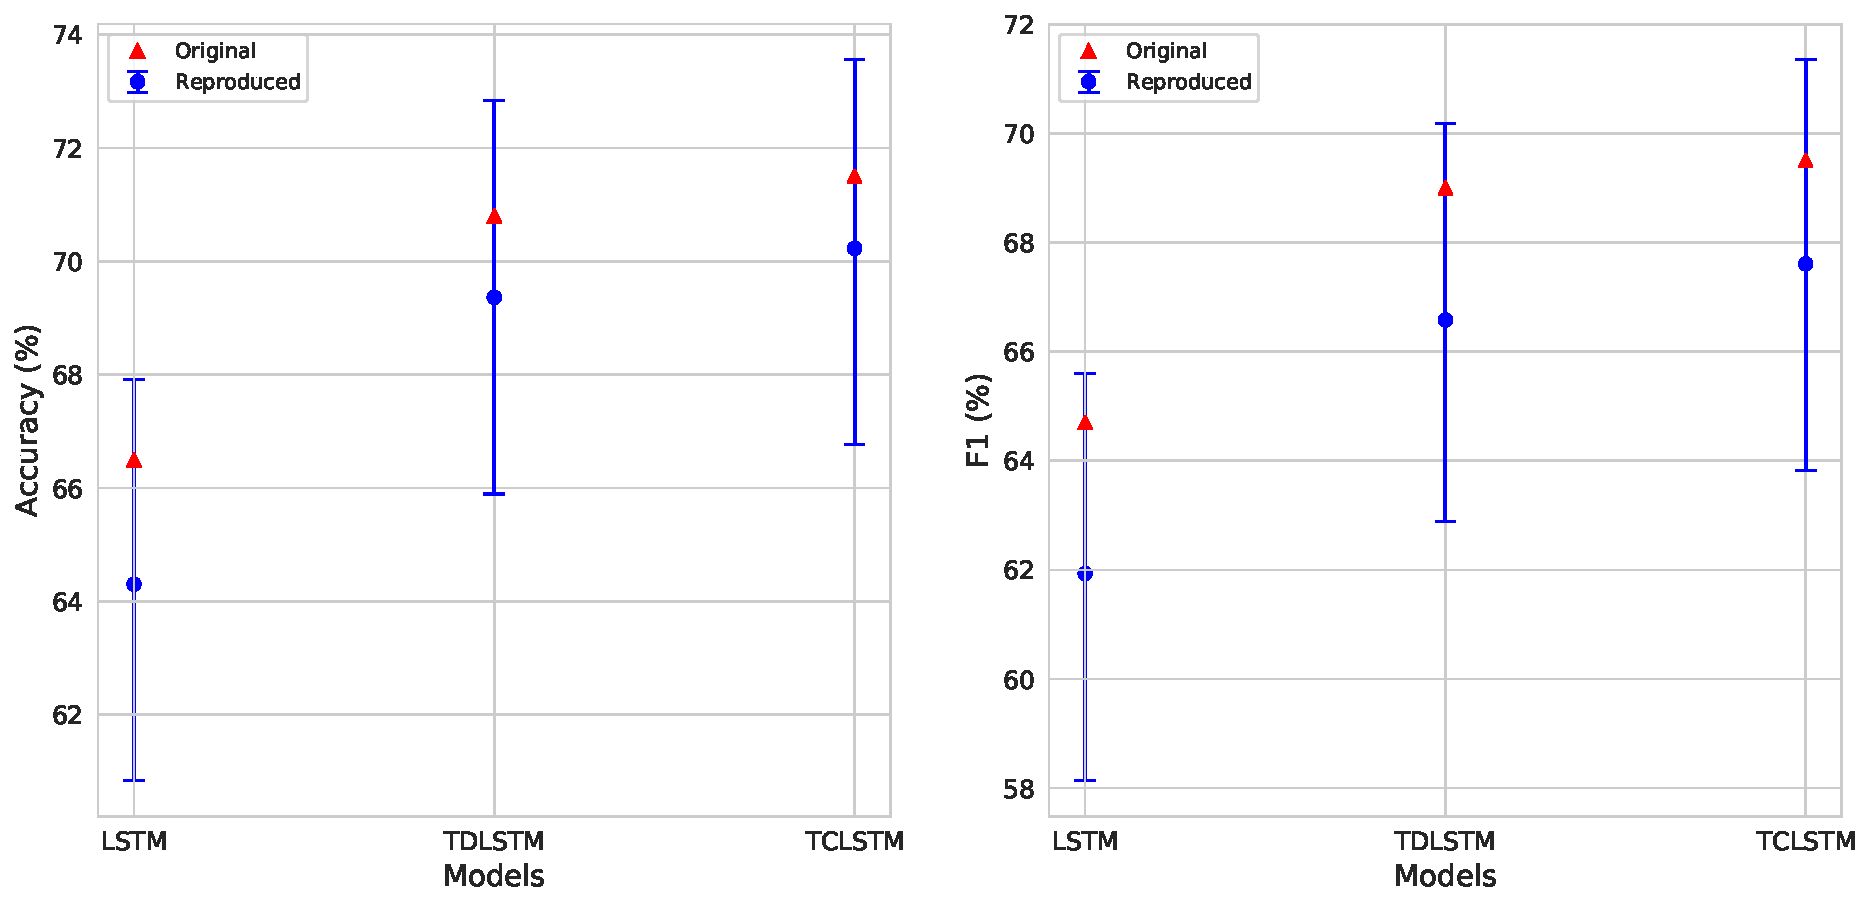
\includegraphics[scale=0.4]{images/reproducibility/tang/LSTM_ACC_F1.pdf}
    \caption{Confidence intervals for the two sided tailed test for the reproduced models of \citet{tang-etal-2016-effective} on both the accuracy and macro F1 metrics.}
    \label{fig:repro_tang_LSTM_ACC_F1}
\end{figure}

Based on the results from table \ref{table:tang_twitter_100_results} it would appear that for many seed values it would not be possible to reproduce these results. To quantify this, the best performing run for each method and metric is compared against all other runs for that method. The number of runs that are significantly worse based on a one sided test corrected using Bonferroni to the best performing run is shown in table \ref{table:tang_significantly_better_runs}. As can be seen out of the $19$ other runs many of them for the macro F1 metric for all methods are significantly different to the best performing run even though they are the same method. This confirms the findings of \citet{reimers-gurevych-2017-reporting} for TDSA for the macro F1 metric whereby random seeds can cause statistically significantly different results for the same method. It further shows that out of all of the methods the TCLSTM would appear to be the least stable, and this could be due to it being the largest, with respect to the number of parameters, of the three methods. From these findings and the distribution of results presented in figure \ref{fig:repro_tang_LSTM_DIST_ACC_F1}, it is believed that a possible reason why others could not reproduce \citep{tay2018learning} or replicate \citep{chen-etal-2017-recurrent} the same scores as the original authors of TDLSTM \citep{tang-etal-2016-aspect} is due to the variance caused by random seeds.

\begin{table}[!h]
    \centering
    \begin{tabular}{|c|c|c|c|}
    \hline
    Metric & LSTM & TDLSTM & TCLSTM  \\
    \hline
    Accuracy & 0 & 0 & 13  \\
    \hline
    F1 & 4 & 2 & 15  \\
    \hline
\end{tabular}
    \caption{The number of runs that the best performing run significantly outperforms using a one side tested and corrected with Bonferroni for accuracy and macro F1.}
    \label{table:tang_significantly_better_runs}
\end{table}

As the methods from \citet{tang-etal-2016-effective} have been reproduced, another of \citet{tang-etal-2016-effective} experiments is repeated and enhanced. The original experiment compares SSWE, GloVe Twitter 50, 100 and 200 embeddings of which both of these embeddings are either type or type and task specific. Thus the experiment is enhanced to include the GloVe 300 dimension non-task nor type specific embedding, that has been already tested in numerous other experiments in this section (see tables \ref{table:repro_vo_word_embeddings_results} and \ref{table:repro_vo_word_embedding_sig_fold_count} for example). The results on the test (validation) set of \citet{dong-etal-2014-adaptive} Twitter dataset can be seen in table \ref{table:repro_tang_test_embedding_scores} (appendix \ref{appendix_reproducibility_tables} table \ref{table:repro_tang_val_embedding_scores}). The findings are slightly different from the original found in figure of \citet{tang-etal-2016-effective}. In comparison \citet{tang-etal-2016-effective} found the TDLSTM to be worse than TCLSTM on all accuracy scores, which is not the case here. Additionally \citet{tang-etal-2016-effective} found SSWE to be worse than GloVe Twitter 50 which again is not found here. These differences in results could be due to the random seeds. More interestingly it is shown that the non-type nor task specific embeddings is better than the all other embeddings for all methods and metrics. Thus showing again that these larger general embeddings can be at least as good as the type and/or task specific embeddings. After performing a one tailed test comparing the GloVe 300 embeddings to all other embeddings for each metric and method they are significantly better in the majority of cases for the test set, as shown in table \ref{table:tang_significantly_better_runs}. The significant results are hard to interpret as the test results suggest that the majority of embeddings for at least TDLSTM and TCLSTM are significantly worse than the GloVe embeddings, but this is not reflected in the validation results as the GloVe embeddings are not significantly better than any of the embeddings\footnote{The p-values from the significant tests can be seen in appendix \ref{appendix_reproducibility_tables} tables \ref{table:repro_tang_embeddings_test_sig} and \ref{table:repro_tang_embeddings_val_sig} for the test and validation results.}. Thus it suggests that perhaps the GloVe embeddings are only weakly better than all other embeddings\footnote{The potential reason for the significance tests to bring back very different results for the test and validation sets could be due to the limitation of the significance test used for the LSTM methods. In this chapter the LSTM based methods when being tested to detect significant differences a particular run from the set of all runs for each compared LSTM method is used. In the majority of cases the median run is used and this to some degree ensures that there is not a bias towards methods that have a large variance in results due to the random seeds. However using the median run or any one run does not take into the account the whole random seed distribution. Thus stating the limitation of the significance test used in this chapter for the LSTM based methods. This limitation could also explain why their is a difference between the significance results of the validation and test set here, as the median run might not be a good representation of all runs results.}.

\begin{table}[!h]
    \centering
    

\begin{tabular}{|c|c|c|c|c|}
\hline
Embedding & Metric &           LSTM &        TDLSTM &        TCLSTM \\
\hline
SSWE & Accuracy &  62.07 \sd{(1.48)} &  66.77$^\star$ \sd{(1.63)} &  65.59$^\star$ \sd{(1.41)} \\
& F1 &  58.37$^\star$ \sd{(2.16)} &  63.35$^\star$ \sd{(1.89)} &  61.96$^\star$ \sd{(1.77)} \\
\hline
Twitter 50 & Accuracy &  61.48$^\star$ \sd{(1.43)} &  65.11$^\star$ \sd{(1.46)} &  64.74$^\star$ \sd{(1.87)} \\
& F1 &  57.12$^\star$ \sd{(2.79)} &  61.67$^\star$ \sd{(2.00)} &  60.72$^\star$ \sd{(2.57)} \\
\hline
Twitter 100 & Accuracy &  62.93 \sd{(0.81)} &  67.23$^\star$ \sd{(1.08)} &  66.74$^\star$ \sd{(1.32)} \\
& F1 &  58.59 \sd{(1.90)} &  63.86$^\star$ \sd{(1.68)} &  63.26$^\star$ \sd{(1.68)} \\
\hline
Twitter 200 & Accuracy &  62.49 \sd{(1.14)} &  68.11$^\star$ \sd{(0.54)} &  67.89 \sd{(0.98)} \\
& F1 &  57.41$^\star$ \sd{(2.81)} &  65.21$^\star$ \sd{(0.94)} &  64.70 \sd{(1.39)} \\
\hline
GloVe 300 & Accuracy &  \textbf{64.73} \sd{(0.76)} &  \textbf{71.04} \sd{(0.68)} &  \textbf{69.22} \sd{(1.27)} \\
& F1 &  \textbf{61.04} \sd{(1.45)} &  \textbf{68.43} \sd{(0.83)} &  \textbf{66.47} \sd{(1.78)} \\
\hline
\end{tabular}
    \caption{Test set mean (standard deviation) results on the \citet{dong-etal-2014-adaptive} Twitter dataset, across various embeddings and methods. The \textbf{bold} values indicate the best embedding score for each method and metric. The $^\star$ indicates when the GloVe embeddings are statistically significantly better (p $\le 0.05$) than the other embedding for that metric and method. The significance test used the one tailed test and used the median best run from the $20$ runs to perform the significance test.}
    \label{table:repro_tang_test_embedding_scores}
\end{table}

\subsection{Conclusion from Reproduction Studies}
It is clear from the large scale NP experiments shown in figures \ref{fig:repro_parameters_c_values_accuracy} (\ref{fig:repro_parameters_c_values_macro_f1}) and \ref{fig:repro_parameters_scaling_accuracy} (\ref{fig:repro_parameters_scaling_macro_f1}) for the accuracy (macro F1) metric, that both the scaling method (if used) and the C-value from the SVM should be stated within the paper. Furthermore the suggestion from \citet{reimers-gurevych-2017-reporting} on reporting multiple runs of the method over different random seed values is required for NN based TDSA methods as the single performance scores can be misleading, which could explain why previous papers obtained different results to the original for the TDLSTM method \citep{chen-etal-2017-recurrent, tay2018learning}. For the first time, it has been shown in this section that scaling method, C-value of the SVM, and random seeds make a significant difference for TDSA methods. 

Additionally within this section it has also been shown that general word embeddings (300 dimension GloVe embeddings) can perform as well as the type and/or task specific embeddings. This has been shown for the NP methods \citep{vo2015target}, where as for the LSTM methods \citep{tang-etal-2016-effective} they tend to prefer the general GloVe embeddings. From this it shows that smaller type and/or task specific embeddings can be as useful as larger general embeddings for at least the NP methods. This implies that from an energy efficiency perspective\footnote{Measured by number of parameters. A better measure for efficiency would be Floating Point Operations (FPO) \citep{schwartz2019green}, but \citet{schwartz2019green} did state that the number of parameters is a form of efficiency measure.} it would be of use to train these smaller type and/or task specific embeddings as the methods that use them will be more efficient than if they use the larger general embeddings. Alternatively it suggests that it is not a requirement to create smaller type and/or task specific embeddings. These findings are at least true for TDSA methods applied to the Dong dataset.

\section[Mass Evaluation]{Mass Evaluation\footnote{Within this section the TDParse Plus and Target Dependent Plus methods will also be called TDParse+ and TD+ respectively.}}
\label{section:repro_mass_eval}
% Need to mention here the difference in the datasets in more detail e.g. dataset size etc macro F1 results etc etc

% Furthermore two of the three methods \citep{vo2015target, tang-etal-2016-effective} that were originally only evaluated on Dong dataset were therefore only evaluated on data that contains one target per text, as shown by the ATS value in table \ref{table:repro_dataset_stats}. 

Given the methods from the three reproduced papers, in this section we evaluate the different methods across six different English datasets that are shown in table \ref{table:repro_dataset_stats}. This will be the first TDSA study that has evaluated methods across different types, mediums, and domains, as well as the largest TDSA evaluation with respect to the number of datasets. This study will thus explore whether the three papers' methods perform differently on these various datasets, seeing if any generalise to all datasets. For all methods they will use the same 300 dimension GloVe embedding as it is the most popular and has been shown within the thesis to perform well on data that it was not originally designed for (i.e. social media type data). All methods will use the Spacy tokeniser and the \citet{wang-etal-2017-tdparse} methods will use the TweeboParser \citep{kong-etal-2014-dependency} dependency parser on all datasets\footnote{This is due to the methods requirements of a dependency parser that produces multiple roots.}. For sentiment lexicon based methods, the same lexicons that \citet{wang-etal-2017-tdparse} employed will be used here. For the NP methods, the best performing C-value for each method and dataset for the accuracy metric found through the experiment conducted in figure \ref{fig:repro_parameters_c_values_accuracy} will be used. Also MinMax scaling will be used for all NP methods. The LSTM based methods will use the same setup as that from section \ref{section:repro_lstm}, but the methods will only be run six times for each dataset due to the computational cost\footnote{Six runs was chosen as according to \citet{reimers2018comparing} as it will allow future researches to compare results using significance tests that take all six runs into account. This test was not used in this chapter as neural methods that require running multiple runs are compared to non-neural methods that do not, and there is no literature that is known to the author that states how to compare multiple run performances to single run performances.}. Further, for all of the LSTM methods the mean result from the six runs will be reported unless otherwise stated. For the NP methods only the two top performing methods are evaluated, again to save on computational cost while still allowing us to compare methods that do and do not use sentiment lexicons. 

% That the addition of sentiment lexicons does not help that much nor does the dependency parser.
The accuracy and macro F1 results on the test set for all datasets can be seen in tables \ref{table:repro_mass_eval_acc} and \ref{table:repro_mass_eval_macro_f1}. The statistically significant results comparing each method can be seen for both metrics in figure \ref{figure:repro_mass_eval_test_sig_results}, for the LSTM methods the median best performing run based on the accuracy metric is used to compare to all other methods. From these results it is clear that the NP methods are by far the better set of methods. Additionally it can be seen that adding sentiment lexicons (NP methods with a `+' in their name) only marginally improve results on some datasets and at most significantly better on one dataset. These findings are also similar when comparing the non-dependency parser approaches (TD and TD+ methods) with those that do use a dependency parser (TDParse and TDParse+), whereby they perform almost as well as each other. Both of these findings show, for at least the methods tested here, that using additional resources such as sentiment lexicons or a dependency parser do not make a large significant difference in results and are thus not needed.

\begin{table}[!h]
    \centering
    
\begin{tabular}{|c|c|c|c|c|c|c|c|}
  \hline
  &   D &  E &  L &  M &  R &  Y &   Mean \\
 \hline
LSTM &  \underline{64.57} &     \underline{47.85} &   59.90 &     71.04 &       \underline{68.63} &      \underline{63.33} &  \underline{62.55} \\
 \hline
TDLSTM &  \textbf{71.12} &     \textbf{57.50} &   61.76 &     \underline{70.52} &       73.56 &      64.17 &  66.44 \\
  \hline
TCLSTM &  68.98 &     57.40 &   \underline{56.77} &     70.77 &       71.85 &      66.81 &  65.43 \\
   \hline
TD &  68.50 &     57.22 &   66.14 &     73.45 &       77.32 &      82.50 &  70.86 \\
   \hline
TD+ &  70.23 &     53.21 &   \textbf{68.97} &     \textbf{74.37} &       78.04 &      81.67 &  71.08 \\
    \hline
TDParse &  67.77 &     57.46 &   67.08 &     73.96 &       77.95 &      79.58 &  70.63 \\
    \hline
TDParse+ &  69.36 &     56.12 &   68.50 &     73.35 &       \textbf{78.30} &      \textbf{83.33} &  \textbf{71.49} \\
\hline
Mean &  68.65 &     55.25 &   64.16 &     72.49 &       75.09 &      74.48 &  - \\
\hline
\multicolumn{8}{|p{11.5cm}|}{\centering D=Dong, E=Election, L=Laptop, M=Mitchell, R=Restaurant, Y=YouTuBean}\\
\hline
\end{tabular}
    \caption{Accuracy results on the test sets of each dataset. For the LSTM based methods this is the mean accuracy result. The mean accuracy across all datasets for each method is in the right most column. Where the \textbf{bold} and \underline{underlined} values indicate the best and worst methods for each dataset and the overall mean accuracy, respectively. The mean accuracy score for each dataset is in the last row.}
    \label{table:repro_mass_eval_acc}
\end{table}

\begin{table}[!h]
    \centering
    \begin{tabular}{|c|c|c|c|c|c|c|c|}
  \hline
  &   D &  E &  L &  M &  R &  Y &   Mean \\
 \hline
 LSTM &  \underline{61.58} &     \underline{30.65} &   \underline{41.91} &     35.51 &       \underline{37.15} &      \underline{25.85} &  \underline{38.78} \\
 \hline
 TDLSTM &  \textbf{68.54} &     42.54 &   49.82 &     \underline{29.67} &       56.66 &      28.98 &  46.04 \\
 \hline
 TCLSTM &  65.92 &     43.57 &   45.04 &     38.42 &       53.54 &      36.83 &  47.22 \\
 \hline
 TD &  65.27 &     46.60 &   57.86 &     48.98 &       63.17 &      \textbf{74.80} &  59.45 \\
 \hline
 TD+ &  67.36 &     44.52 &   \textbf{62.33} &     48.08 &       64.44 &      72.90 &  59.94 \\
 \hline
 TDParse &  64.33 &     \textbf{46.64} &   59.23 &     48.58 &       64.66 &      70.05 &  58.91 \\
 \hline
 TDParse+ &  66.36 &     46.30 &   61.89 &     \textbf{51.17} &       \textbf{65.26} &      74.46 &  \textbf{60.91} \\
 \hline
 Mean &  65.62 &     42.98 &   54.01 &     42.92 &       57.84 &      54.84 &  - \\
 \hline
\multicolumn{8}{|p{11.5cm}|}{\centering D=Dong, E=Election, L=Laptop, M=Mitchell, R=Restaurant, Y=YouTuBean}\\
\hline
 \end{tabular}
    \caption{Macro F1 results on the test sets of each dataset. For the LSTM based methods this is the mean macro F1 result. The mean macro F1 across all datasets for each method is in the right most column. Where the \textbf{bold} and \underline{underlined} values indicate the best and worst methods for each dataset and the overall mean macro F1, respectively. The mean macro F1 score for each dataset is in the last row.}
    \label{table:repro_mass_eval_macro_f1}
\end{table}

\begin{figure}[!h]
    \centering
    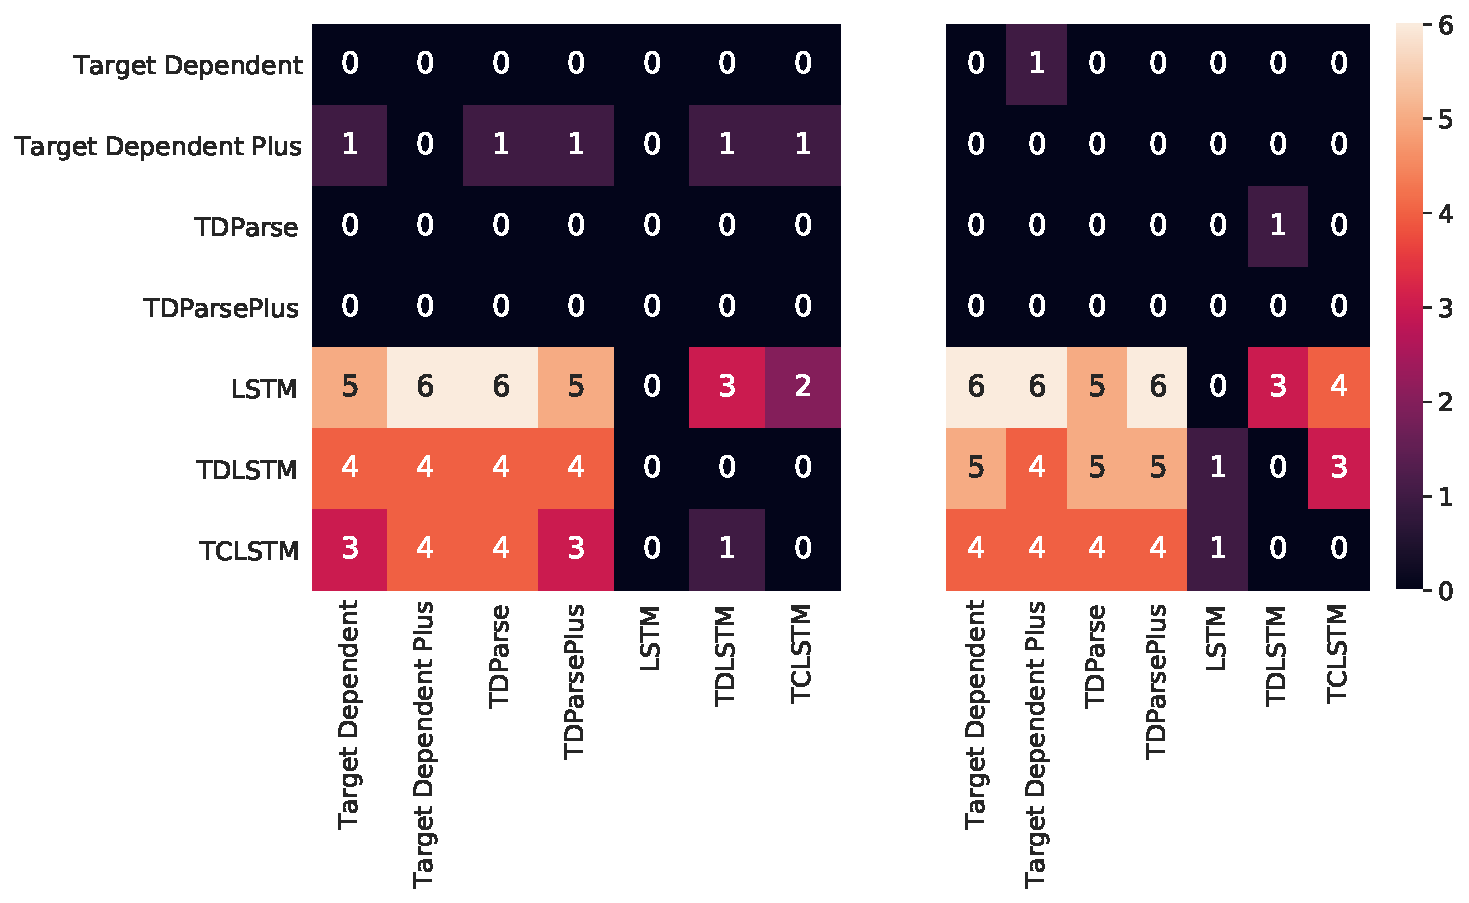
\includegraphics[scale=0.4]{images/reproducibility/Sig_Test.pdf}
    \caption{The number of datasets where the column methods are statistically significantly better than the row methods, corrected using Bonferroni. The left and right heatmap represent the accuracy and macro F1 scores. This is using the median performing run based on the accuracy metric for the LSTM methods.}
    \label{figure:repro_mass_eval_test_sig_results}
\end{figure}

% It has been shown that some of the LSTM methods perform worse than the baseline sentence method.
Between the LSTM based methods it is clear that on average the target specific LSTM based methods (TDLSTM and TCLSTM) are better than the sentence level classifier baseline (LSTM). However the TDLSTM and TCLSTM are worse than the LSTM on the Mitchell dataset, and the TCLSTM is worse than LSTM on the Laptop dataset when using the accuracy metric. Both of these represent a failure for the target specific methods as they are beaten by a much simpler baseline. This finding demonstrates one reason why it is important to test methods across a wide range of datasets.

% LSTM methods perform worse when low resourced or highly unbalanced.
Comparing the LSTM based methods to the NP it is clear that the LSTM based methods perform better in comparison to NP on larger datasets e.g. Election and Dong. Whereas the NP methods in comparison perform much better on the smaller datasets (YouTuBean), further they also perform better with respect to macro F1 scores. The macro F1 results suggest that the LSTM methods perform poorly on datasets that are highly un-balanced e.g. Mitchell and this gets worse when the dataset is small and un-balanced e.g. YouTuBean. Furthermore for the YouTuBean and the Mitchell datasets the macro F1 score distribution is quite large, as shown in figure \ref{figure:repro_LSTM_TEST_F1}\footnote{For the distribution of the accuracy scores for the LSTM methods see figure \ref{figure:repro_LSTM_TEST_ACC} in appendix \ref{appendix_reproducibility_images}.}, in comparison to all of the other datasets. This suggests that the LSTM methods are more sensitive to random seed/initialisation for smaller and un-balanced datasets. To overcome the overfitting to particular labels, re-sampling techniques such as under or over sampling could be of use. In some prior work it has been shown that transfer learning from a document sentiment dataset has greatly improved the macro F1 score for LSTM methods \citep{he-etal-2018-exploiting}. However more work investigating how to improve NN based TDSA methods with respect to highly un-balanced and/or low resourced corpora should be investigated. Lastly from the significance results it is clear that the NP methods do not struggle to beat the LSTM sentence level classifier baseline.

\begin{figure}[!h]
    \centering
    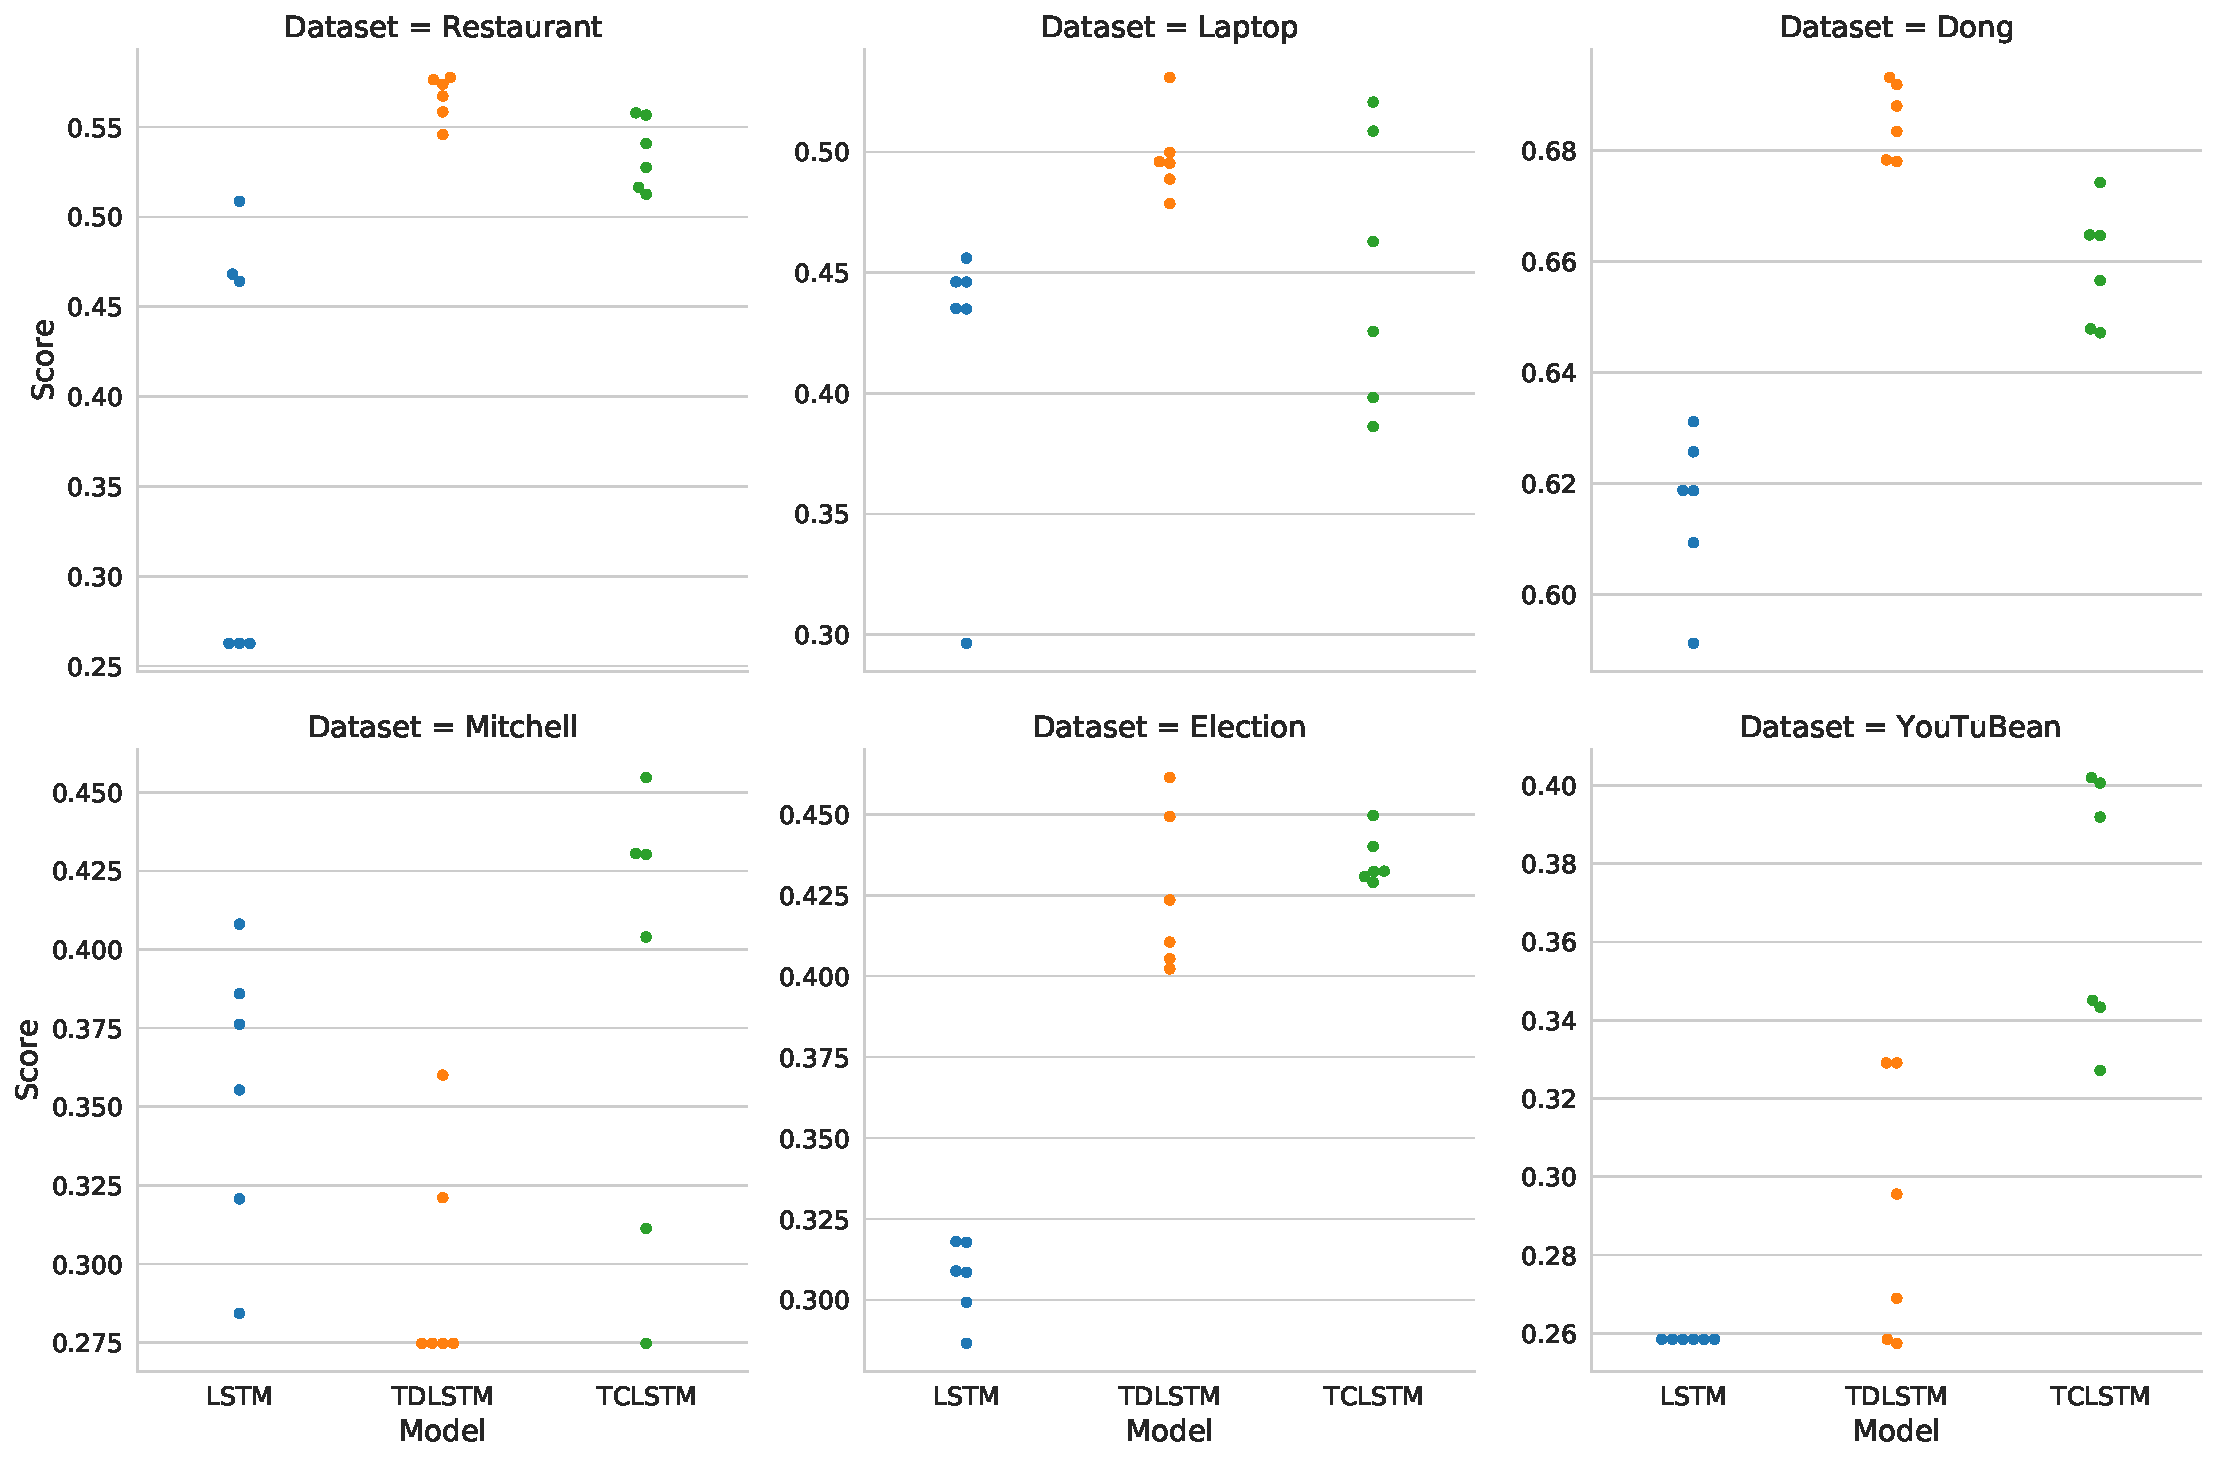
\includegraphics[scale=0.3]{images/reproducibility/LSTM_Test_F1.pdf}
    \caption{Distribution of macro F1 scores from the six runs for each LSTM method and test dataset.}
    \label{figure:repro_LSTM_TEST_F1}
\end{figure}

% Stating that the variation in datasets, that it would appear that the methods are more affected by size, DS, and class distribution rather than type, medium, and domain
From a performance perspective in general the hardest dataset, according to accuracy, is the Election one, even though it is the largest by a large margin. The reason for its difficulty is believed to stem from the fact it has a large distribution of samples in $DS_2$ and $DS_3$, as \citet{wang-etal-2017-tdparse} suggest that $DS_3$ is the most difficult scenario. It also appears that the methods are less affected by the type, domain, or medium that dataset has come from but rather the size, \textit{DS} distribution, and sentiment class distribution. This is observed as methods that do incorporate type specific features e.g. a Twitter based dependency parser perform worse in rank terms on the social media type datasets some of the time than on the non-social media type datasets. For example, TDParse performs worse on Dong but better on Laptop compared to TD.

% Showing that by using a better seed value the LSTM methods are stil worse.
It is worth noting that to a large extent the NP methods have an advantage over the LSTM methods as the C-value which is significant has been tuned for each dataset and method, where as the LSTM methods have had no tuning. However some of the NP methods still perform better than the TDLSTM results for the Restaurant dataset from prior work, as shown by table \ref{table:repro_tang_authors_differences}. This is highlighted as these other prior works may have tuned the TDLSTM or found a better seed value than in the evaluation performed here. To give the LSTM methods an increased advantage over the NP methods, due to the NP methods having their C-values tuned, the LSTM methods have been recompared to the NP whereby the best performing run/seed value is used. Figures \ref{figure:repro_mass_eval_max_acc_test_sig_results} and \ref{figure:repro_mass_eval_max_f1_test_sig_results} show the number of datasets that the methods are significantly better on using the best performing run based on the accuracy and macro F1 metric. However with this increased advantage for the LSTM methods it can be seen that the NP methods are still significantly better and the change in the heatmap compared to figure \ref{figure:repro_mass_eval_test_sig_results} is minimal. 

\begin{figure}[!h]
    \centering
    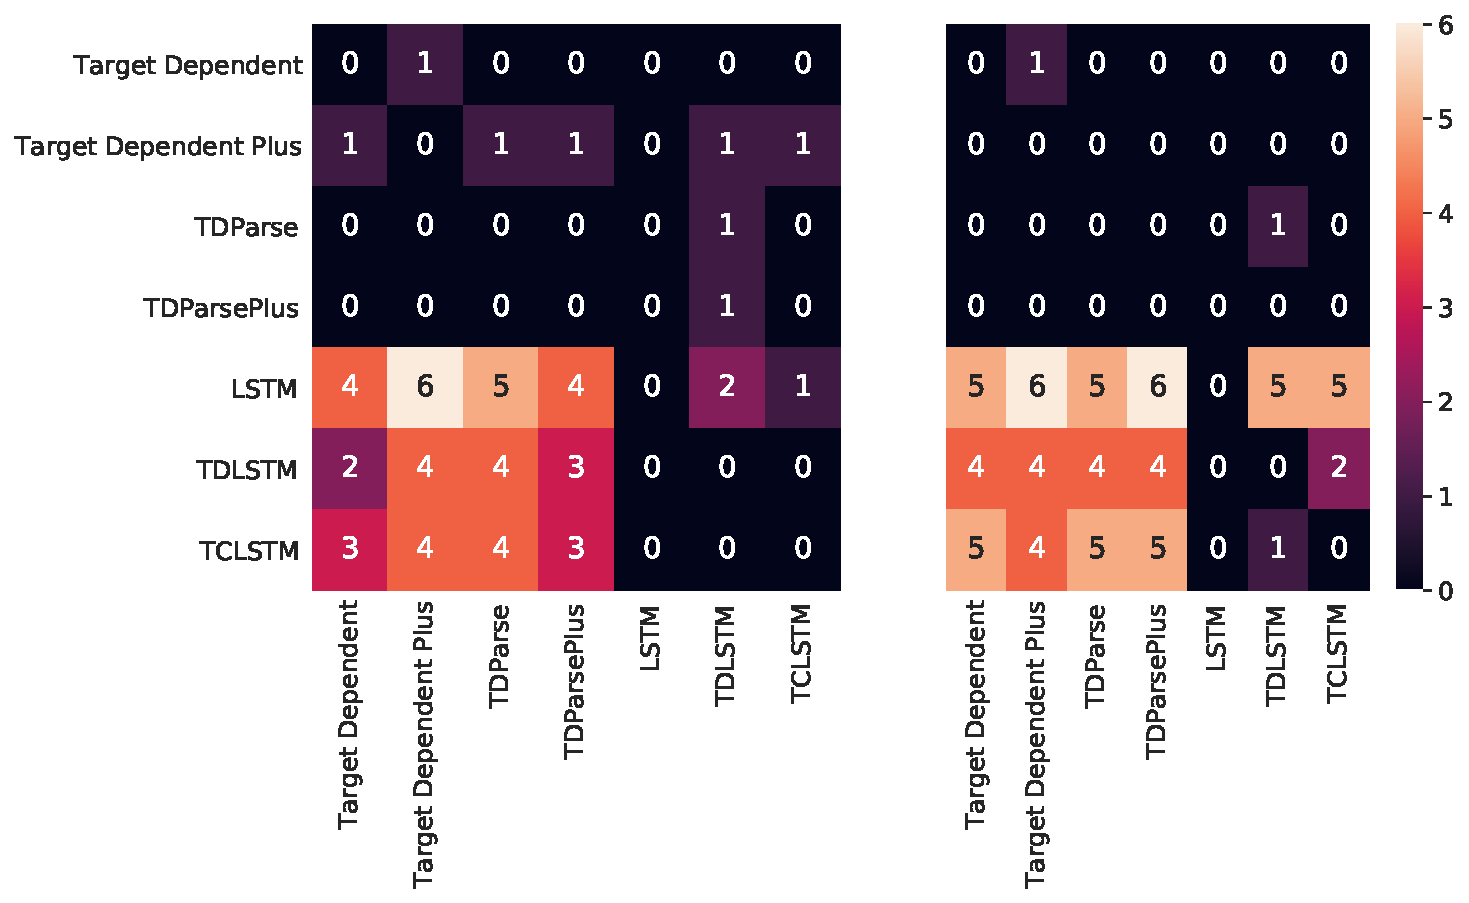
\includegraphics[scale=0.4]{images/reproducibility/Sig_Max_Acc_Test.pdf}
    \caption{The number of datasets where the column methods are statistically significantly better than the row methods, corrected using Bonferroni. The left and right heatmaps represent the accuracy and macro F1 scores. This is using the best performing run based on the \textbf{accuracy metric} for the LSTM methods.}
    \label{figure:repro_mass_eval_max_acc_test_sig_results}
\end{figure}

\begin{figure}[!h]
    \centering
    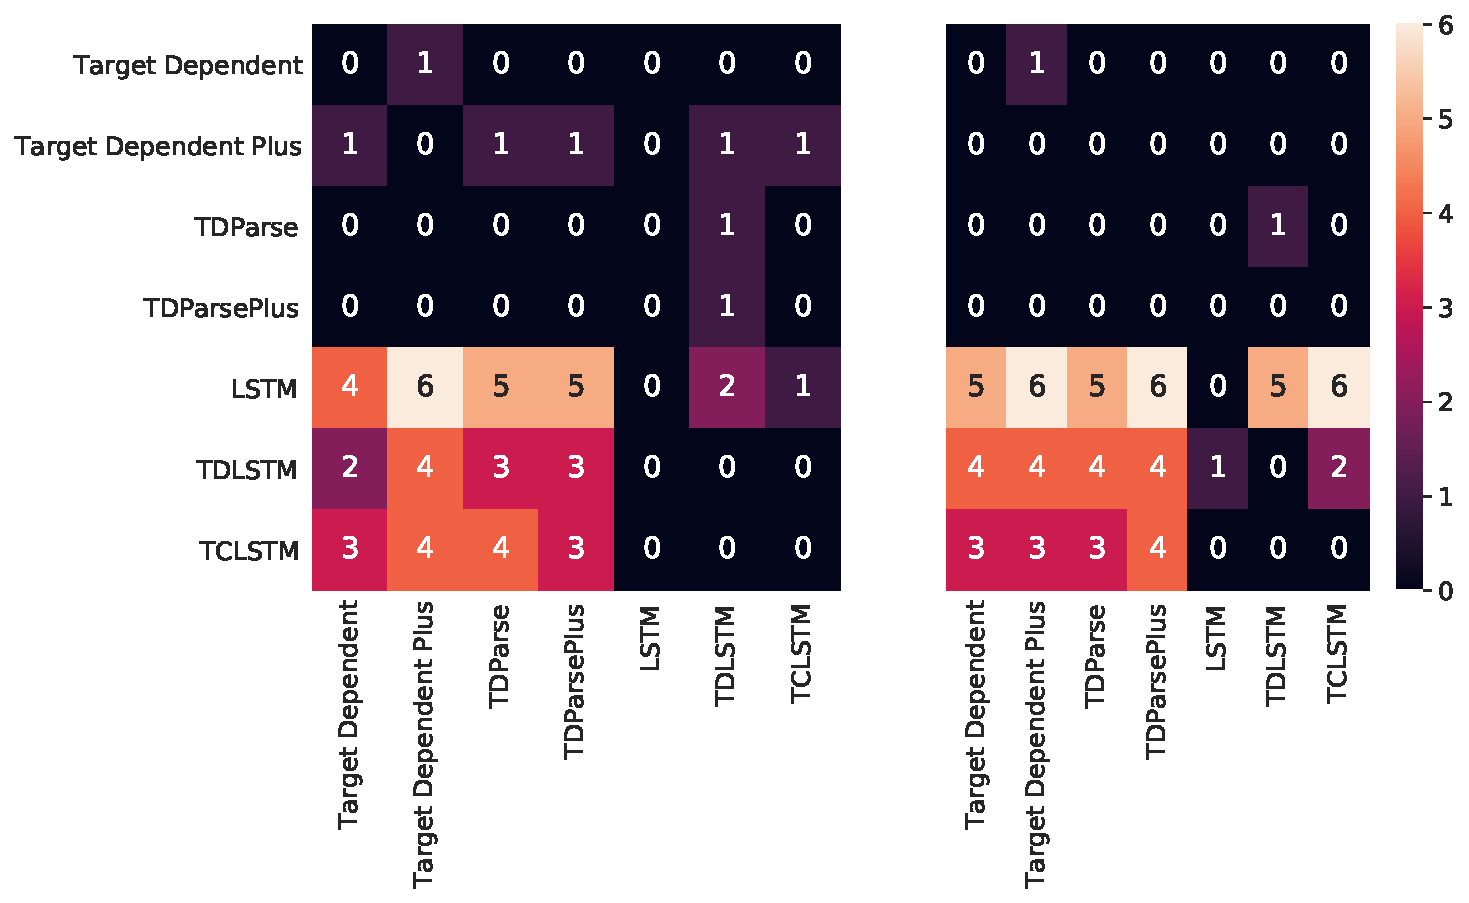
\includegraphics[scale=0.4]{images/reproducibility/Sig_Max_F1_Test.pdf}
    \caption{The number of datasets where the column methods are statistically significantly better than the row methods, corrected using Bonferroni. The left and right heatmaps represent the accuracy and macro F1 scores. This is using the best performing run based on the \textbf{macro F1 metric} for the LSTM methods.}
    \label{figure:repro_mass_eval_max_f1_test_sig_results}
\end{figure}

As stated earlier, the LSTM methods tend to perform worse on smaller datasets. Thus to test how this low resource setting affects LSTM and NP methods on a larger scale all of the datasets training set sizes have been reduced to the same size as YouTuBean training set size, which is the smallest dataset within the evaluated datasets\footnote{For the \citet{dong-etal-2014-adaptive} Twitter dataset instead of training the NP methods using the median pooled approach due to the `same target multiple appearance' issue \citet{wang-etal-2017-tdparse}. All methods including the NP methods will use the first appearance of the target in the text. This was done due to compatibility reason between the NP and LSTM methods after splitting the training dataset.}. Further for the LSTM based methods this new reduced training set size also means that 20\% of that training set is used as a validation set for early stopping. All methods are retrained using the same settings. As the YouTuBean dataset has already been evaluated and would not be affected by this new size reduction it will not be included in the analysis of these experiments. The accuracy and macro F1 results on the test sets for these datasets can be seen in tables \ref{table:repro_small_mass_eval_acc} and \ref{table:repro_small_mass_eval_macro_f1}. The statistically significant results comparing each method can be seen for both metrics in figure \ref{figure:repro_mass_eval_small_test_sig_results}, for the LSTM methods the median best performing run based on the accuracy metric is used to compare to all other methods.

% It can be seen in this more low resourced setting that the sentiment lexicons do appear to be beneifical within the review domain. This is probably because the Hu and Liu sentiments are form the review type

\begin{table}[!h]
    \centering
    \begin{tabular}{|c|c|c|c|c|c|c|}
\hline
Method  &   D &  E &  L &  M &  R  &   Mean \\
\hline
LSTM &  \underline{50.00} &     \underline{46.20} &   53.11 &     \underline{70.11} &       \underline{65.00} &  \underline{56.88} \\
\hline  
TDLSTM &  50.02 &     49.00 &   52.25 &     \underline{70.11} &       \underline{65.00} &  57.28 \\
\hline  
TCLSTM &  51.01 &     49.91 &   \underline{50.89} &     \underline{70.11} &       \underline{65.00} &  57.39 \\
\hline   
TD &  65.75 &     \textbf{51.59} &   60.82 &     \textbf{72.75} &       72.50 &  64.68 \\
\hline    
TD+ &  \textbf{66.62} &     49.08 &   \textbf{64.58} &     72.64 &       74.29 &  65.44 \\
\hline    
TDParse &  65.61 &     \textbf{51.59} &   60.82 &     72.44 &       74.11 &  64.91 \\
\hline    
TDParse+ &  65.75 &     50.45 &   64.26 &     71.94 &       \textbf{74.91} &  \textbf{65.46} \\
\hline
Mean &  59.25 &     49.69 &   58.10 &     71.44 &       70.11 &  - \\
\hline
\multicolumn{7}{|p{9.5cm}|}{\centering D=Dong, E=Election, L=Laptop, M=Mitchell, R=Restaurant, Y=YouTuBean}\\
\hline
\end{tabular}
    \caption{Using the smaller training datasets, the accuracy results on the test sets of each dataset. For the LSTM based methods this is the mean accuracy result. The mean accuracy across all datasets for each method is in the right most column. Where the \textbf{bold} and \underline{underlined} values indicate the best and worst methods for each dataset and the overall mean accuracy, respectively. The mean accuracy score for each dataset is in the last row.}
    \label{table:repro_small_mass_eval_acc}
\end{table}

\begin{table}[!h]
    \centering
    \begin{tabular}{|c|c|c|c|c|c|c|}
\hline
Method  &   D &  E &  L &  M &  R  &   Mean \\
\hline
LSTM &  \underline{22.22} &     27.15 &   \underline{23.47} &     \underline{27.48} &       \underline{26.26} &  \underline{25.32} \\
\hline
TDLSTM &  22.29 &     \underline{26.14} &   29.12 &     \underline{27.48} &       \underline{26.26} &  26.26 \\
\hline
TCLSTM &  27.65 &     32.46 &   32.59 &     \underline{27.48} &       \underline{26.26} &  29.29 \\
\hline
TD &  \textbf{62.48} &     39.18 &   52.11 &     \textbf{45.73} &       54.66 &  50.83 \\
\hline
TD+ &  62.44 &     39.34 &   \textbf{57.71} &     41.41 &       58.65 &  51.91 \\
\hline
TDParse &  62.43 &     \textbf{39.39} &   51.69 &     44.14 &       57.77 &  51.08 \\
\hline
TDParse+ &  61.36 &     38.25 &   56.86 &     44.58 &       \textbf{60.14} &  \textbf{52.24} \\
\hline
Mean &  45.84 &     34.56 &   43.36 &     36.90 &       44.29 &  - \\
\hline
\multicolumn{7}{|p{9.5cm}|}{\centering D=Dong, E=Election, L=Laptop, M=Mitchell, R=Restaurant, Y=YouTuBean}\\
\hline
\end{tabular}
    \caption{Using the smaller training datasets, the macro F1 results on the test sets of each dataset. For the LSTM based methods this is the mean macro F1 result. The mean macro F1 across all datasets for each method is in the right most column. Where the \textbf{bold} and \underline{underlined} values indicate the best and worst methods for each dataset and the overall mean macro F1, respectively. The mean macro F1 score for each dataset is in the last row.}
    \label{table:repro_small_mass_eval_macro_f1}
\end{table}

\begin{figure}[!h]
    \centering
    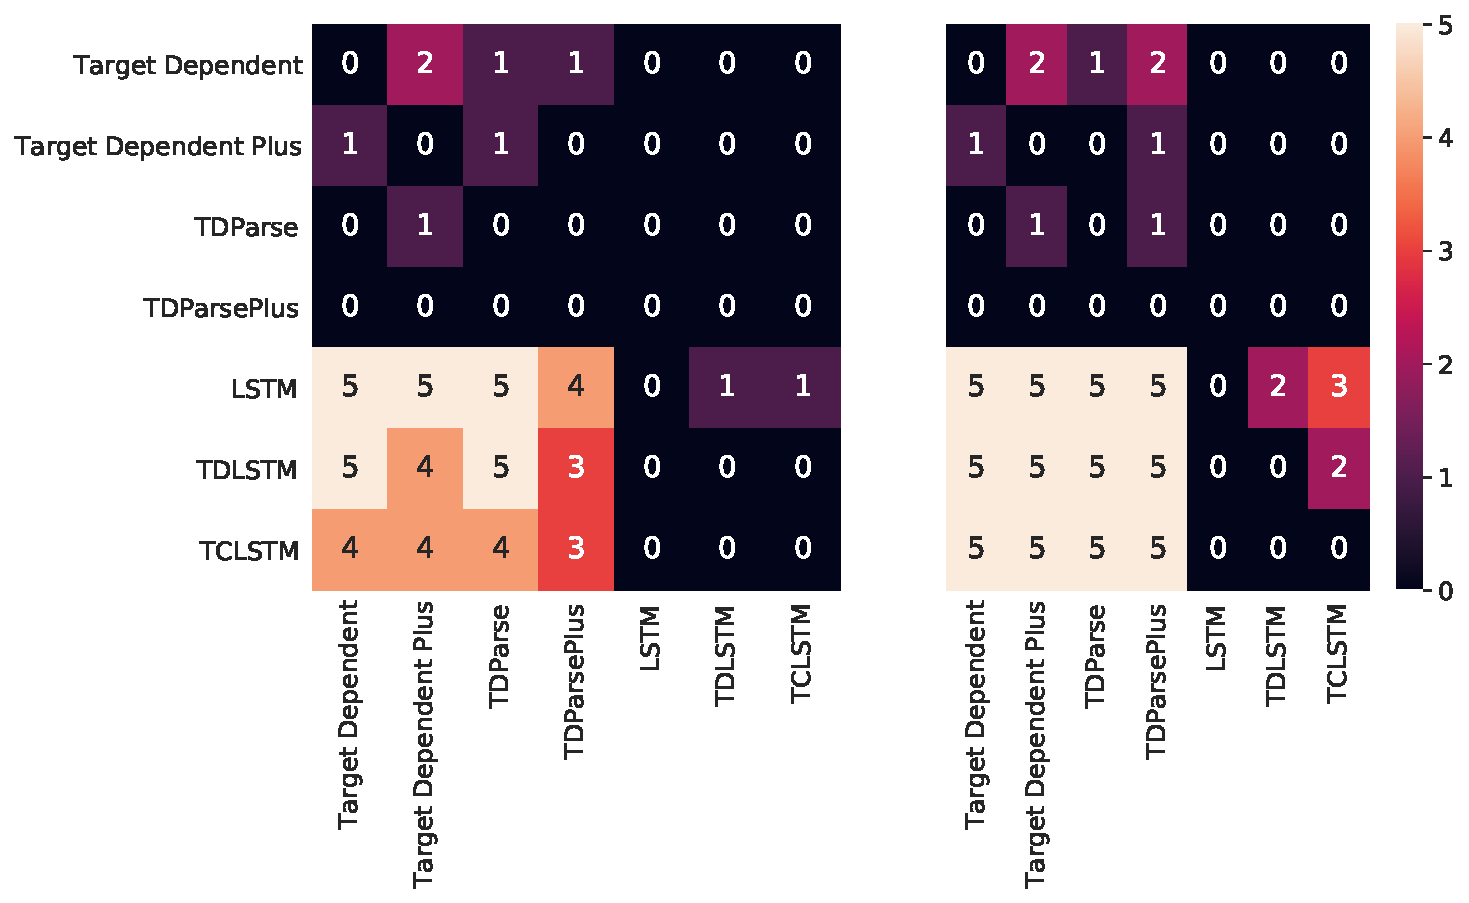
\includegraphics[scale=0.4]{images/reproducibility/Small_Sig_Test.pdf}
    \caption{Using the smaller training datasets, the values represent number of datasets the column methods are statistically significantly better than the row methods, corrected using Bonferroni. The left and right heatmap represent the accuracy and macro F1 scores. This is using the median performing run based on the accuracy metric for the LSTM methods.}
    \label{figure:repro_mass_eval_small_test_sig_results}
\end{figure}

% In the low resource setting it is more clear that the NP methods perform a lot better. Furthermore they do not overfit to only one sentiment class. Also it is more clear that the sentiment lexicons are more affective in the low resource setting if the lexicon used is close to the dataset applied on.
From the results it is clear that the NP methods perform the best in this low resource setting. The datasets that the LSTM methods did perform better on (Dong and Election), they are now worse on. The target specific LSTM methods (TDLSTM and TCLSTM) now have very similar performance to the sentence level LSTM method, which was not the case for all of the results in the normal resource setting. Furthermore the LSTM methods have exceptionally poor performance on the macro F1 results, so much so that all NP methods are significantly better on all datasets compared to all of the LSTM methods. The macro F1 results are broken down into F1 scores for each of the sentiment classes positive, neutral, and negative which can be see in tables \ref{table:repro_small_mass_eval_pos_f1}, \ref{table:repro_small_mass_eval_neu_f1}, and \ref{table:repro_small_mass_eval_neg_f1}. From these results it is clear that for the datasets that are most un-balanced, the LSTM methods can only predict the majority class correctly e.g neutral for Mitchell and positive for Restaurant. In comparison the NP methods are much less affected by the un-balanced datasets and can predict at least one sample correctly for all sentiment classes for all datasets, which only the TCLSTM method can do for the Laptop and Dong dataset. 

In the low resource setting for NP methods, it is still clear that the addition of a dependency parser (TDParse and TDParse+)  does not make a large significance difference. In comparison it is more clear that for the dataset from the written medium and coming from the review domain (Laptop and Restaurant) that using sentiment lexicons makes a large difference for both the accuracy and macro F1 metrics. This result is most likely due to the limited data and thus the sentiment lexicon act as a good inductive bias. The reason why the lexicon based methods perform well only on these datasets is most likely due to one of the lexicons coming from that medium and type, \citet{hu2004mining} sentiment lexicon, where as the other lexicons used are more general. This shows that in a low resource setting sentiment lexicons are useful, only if they come from the same type and medium, as the YouTuBean which comes from the review type but not written medium does not benefit from the sentiment lexicons as shown in table \ref{table:repro_mass_eval_acc} and \ref{table:repro_mass_eval_macro_f1}\footnote{For the TDParse method there is an increase for both the accuracy and macro F1 metric when adding sentiment lexicon. This is not the case for the TD method whereby adding sentiment lexicons harms the performance for both accuracy and macro F1.}.

\begin{table}[!h]
    \centering
    \begin{tabular}{|c|c|c|c|c|c|c|}
\hline
Method  &   D &  E &  L &  M &  R  &   Mean \\
\hline
LSTM &   \underline{0.00} &      \underline{0.00} &   \underline{69.43} &      \underline{0.00} &       \underline{78.79} &  \underline{29.64} \\
\hline
TDLSTM &   \underline{0.00} &      \underline{0.00} &   70.53 &      \underline{0.00} &       \underline{78.79} &  29.86 \\
\hline
TCLSTM &  10.40 &      \underline{0.00} &   70.28 &      \underline{0.00} &       \underline{78.79} &  31.89 \\
\hline
TD &  57.88 &      6.38 &   76.73 &     \textbf{41.40} &       84.00 &  \textbf{53.28} \\
\hline
TD+ &  54.23 &     \textbf{12.43} &   78.79 &     31.40 &       84.96 &  52.36 \\
\hline
TDParse &  \textbf{58.20} &      6.83 &   76.82 &     38.30 &       84.57 &  52.94 \\
\hline
TDParse+ &  52.63 &      5.87 &   \textbf{79.31} &     38.35 &       \textbf{85.17} &  52.27 \\
\hline
\end{tabular}
    \caption{Using the smaller training datasets, the F1 results for the \textbf{positive class} on the test sets of each dataset. For the LSTM based methods this is the mean F1 result. The mean F1 across all datasets for each method is in the right most column. Where the \textbf{bold} and \underline{underlined} values indicate the best and worst methods for each dataset and the overall mean F1, respectively.}
    \label{table:repro_small_mass_eval_pos_f1}
\end{table}

\begin{table}[!h]
    \centering
    \begin{tabular}{|c|c|c|c|c|c|c|}
\hline
Method  &   D &  E &  L &  M &  R  &   Mean \\
\hline
LSTM &  \underline{66.67} &     20.71 &    \underline{0.00} &     \underline{82.43} &        \underline{0.00} &  33.96 \\
\hline
TDLSTM &  66.69 &     \underline{13.70} &   \underline{0.00} &     \underline{82.43} &        \underline{0.00} &  \underline{32.56} \\
\hline
TCLSTM &  67.02 &     34.57 &    0.39 &     \underline{82.43} &        \underline{0.00} &  36.88 \\
\hline
TD &  72.87 &     52.06 &   33.62 &     83.68 &       31.91 &  54.83 \\
\hline
TD+ &  \textbf{73.99} &     48.45 &   \textbf{42.80} &     \textbf{83.74} &       37.54 &  \textbf{57.31} \\
\hline
TDParse &  72.41 &     \textbf{52.79} &   31.62 &     83.38 &       33.21 &  54.68 \\
\hline
TDParse+ &  73.37 &     50.98 &   41.11 &     83.15 &       \textbf{37.67} &  57.26 \\
\hline
\end{tabular}
    \caption{Using the smaller training datasets, the F1 results for the \textbf{neutral class} on the test sets of each dataset. For the LSTM based methods this is the mean F1 result. The mean F1 across all datasets for each method is in the right most column. Where the \textbf{bold} and \underline{underlined} values indicate the best and worst methods for each dataset and the overall mean F1, respectively.}
    \label{table:repro_small_mass_eval_neu_f1}
\end{table}

\begin{table}[!h]
    \centering
    \begin{tabular}{|c|c|c|c|c|c|c|}
\hline
Method  &   D &  E &  L &  M &  R  &   Mean \\
\hline
LSTM &   \underline{0.00} &     60.75 &    \underline{1.00} &      \underline{0.00} &        0.00 &  \underline{12.35} \\
\hline
TDLSTM &   0.19 &     \textbf{64.72} &   16.82 &      \underline{0.00} &        \underline{0.00} &  16.34 \\
\hline
TCLSTM &   5.54 &     62.81 &   27.09 &      \underline{0.00} &        \underline{0.00} &  19.09 \\
\hline
TD &  56.70 &     59.11 &   45.97 &     12.12 &       48.05 &  44.39 \\
\hline
TD+ &  \textbf{59.09} &     \underline{57.14} &   \textbf{51.53} &      9.09 &       53.46 &  46.06 \\
\hline
TDParse &  56.68 &     58.54 &   46.63 &     10.75 &       55.52 &  45.62 \\
\hline
TDParse+ &  58.09 &     57.90 &   50.15 &     \textbf{12.24} &       \textbf{57.58} &  \textbf{47.19} \\
\hline
\end{tabular}
    \caption{Using the smaller training datasets, the F1 results for the \textbf{negative class} on the test sets of each dataset. For the LSTM based methods this is the mean F1 result. The mean F1 across all datasets for each method is in the right most column. Where the \textbf{bold} and \underline{underlined} values indicate the best and worst methods for each dataset and the overall mean F1, respectively.}
    \label{table:repro_small_mass_eval_neg_f1}
\end{table}

\section{Conclusion}
Within this chapter, the reproduction studies have found, for the first time, that for NP methods within TDSA both scaling features and C-values within SVMs are statistically significant factors. Furthermore it is recommended that these factors are reported within a structured format like that suggested by \citet{dodge-etal-2019-show} within Appendix B-D with all other relevant information about the method. For TDSA LSTM based methods it has been shown for at least one metric (macro F1) that they can be statistically significantly affected by random seeds for the first time, this has been shown previously by \citet{reimers-gurevych-2017-reporting} for neural sequence labelling methods. Thus it is recommended to follow \citet{reimers-gurevych-2017-reporting} advice on reporting and comparing distribution of scores that are generated from the LSTM methods by different random seeds. 

Additionally the reproduction studies found that for NP the larger general embedding (300 dimension GloVe) can perform as well as the type and/or task specific embeddings that the original method used \citep{vo2015target}. This implies that from an energy saving perspective it can be useful to train smaller more relevant embeddings for NP methods. While the LSTM methods preferred the larger general embedding, suggesting there is no requirement to train smaller more relevant embeddings. However these findings have only been tested on NP and LSTM methods on one Twitter dataset (Dong \citep{dong-etal-2014-adaptive}), it would be beneficial to broaden the experiment to more datasets. These findings so far in the conclusion have allowed us to answer \rqref{rq:lessons} `what lesson can be learned from reproducing a method within TDSA?’.

The following findings help to answer \rqref{rq:generalisable} `how generalisable are existing methods within TDSA?'. It is found that in general the NP methods are better than the LSTM, but the LSTM methods can perform better in general on larger datasets. Thus showing to some degree that there is no one winning method. While testing methods across various datasets that have different domains, types, and mediums it is found that on the standard datasets sizes these factors do not differentiate the methods. Rather, testing methods on datasets that vary by size, sentiment class distribution, and Distinct Sentiment (\textit{DS}) distribution are the most influential factors. From these factors it is shown that in general all methods perform badly when the dataset contains a large distribution of samples from $DS_3$ and $DS_2$. Further the LSTM methods are badly affected when the datasets are highly un-balanced and/or small, in these cases the NP methods are highly recommend. It was found in the low resource setting, that the inductive bias of sentiment lexicons in NP methods is useful, only if the sentiment lexicon comes from the same type and medium. Neither, the use of sentiment lexicons nor the features from a dependency parser are of significant use in the higher resource setting. Lastly it was found in some cases the target specific methods (TDLSTM and TCLSTM) were no better than the baseline (LSTM) method. This was not found in the original paper \citep{tang-etal-2016-effective}, as the datasets this was found on was not used by the original paper, demonstrating the need to test methods across varying datasets. From these findings it is recommended that future work investigates how to improve TDSA methods within the low resource and/or unbalanced setting especially for NN/LSTM based methods. \citet{he-etal-2018-exploiting} has already shown that transfer learning from document level sentiment analysis can improve LSTM based methods performance on unbalanced TDSA datasets. Thus transfer learning and or multi-task learning could be a good future direction. 

There are some caveats with the research presented so far on `how generalisable are methods within TDSA?’. Even though it was found that LSTM based methods did not perform as well as the NP methods on small or smaller datasets, this does not mean another different LSTM based method could not perform better. For instance the LSTM methods used did not have any regularisation applied\footnote{This decision was made as the LSTM methods used followed the original design of the LSTM methods \citep{tang-etal-2016-effective}, where the original design did not use regularisation.}, where regularisation methods such as variational dropout \citep{gal2016theoretically} and label smoothing \citep{szegedy2016rethinking} have been shown to enhance the performance of neural network based methods \citep{gal2016theoretically, song2019attentional}. Furthermore, it should be noted that all findings here are constrained to the English language, thus the findings here are language dependent\footnote{This is highlighted following what has been known as the \#BenderRule \citep{bender2019rule}, which re-iterated a point made in prior work \citep{bender2011achieving}, that not stating the language (normally English) the data has come from misleads the reader into thinking the work is language independent.}.\langcorrections{I think this can now be removed as I state this in the introduction.}

% Future work
%As found the LSTM methods perform badly within the low resource setting, to the extent that on highly un-balanced datasets they can only correctly predict one sentiment class. This is in comparison to NP linear based methods that perform much better within the low resource setting. It has been shown previosly that LSTM methods can be grealty improved with respect to highly un-balanced datasets through transfer learning from document sentiment analysis \citep{he-etal-2018-exploiting}. Additionally it has also been shown transfer learning from language modelling can greatly improves results within the low resource setting \citep{howard-ruder-2018-universal}. Thus future work should look at how to improve methods in the low resource and highly un-balanced class settings, of which transfer learning could be a potential solution. 


\chapter[Improving Experimental Methodology for TDSA]{Improving Experimental\\Methodology for TDSA}
\label{chapter:methodology}
\FloatBarrier
\section[Introduction]{Introduction\footnote{All code that creates the evidence for this chapter can be found here: \url{https://github.com/apmoore1/tdsa_comparisons}. Certain sections throughout this chapter may have more specific pointers to python notebooks that created the analyses within that given section.}}
\label{section:aug_introduction}
As clearly shown within table \ref{table:repro_methods_datasets_used} of the reproducibility and generalisability chapter \ref{chapter:reproducibility}, many methods have been created, although they have only been applied to selected datasets. This lack of reporting is further compounded with many prior works only stating accuracy and/or macro F1 scores on the entire dataset. This type of reporting is good at comparing methods generally on these datasets. However having more detailed analysis on different splits of the data or task specific metrics would advance the community in knowing what the methods are not representing, for instance a method could generally perform well but might perform badly when there are lots of targets in one text. Thus the field would benefit generally from detailed error analysis. Some prior works have suggested different TDSA specific splits of the entire dataset to overcome this error analysis deficiency \citep{nguyen-shirai-2015-phrasernn,wang-etal-2017-tdparse,he-etal-2018-effective,yang2018multi}, but few publications since these have used the designed splits and only report the entire dataset score. This causes a major problem within our community, and so `we do not know what we know'. To further expand on the meaning of this, a lot of the methods within the community have general scores that are fairly similar e.g. only showing 3-4\% differences on the Restaurant dataset (table \ref{tab:aug_previous_work_results})\footnote{For an up to date list of papers and scores see \textit{Papers With Code} \url{https://paperswithcode.com/sota/aspect-based-sentiment-analysis-on-semeval}.} but what does that mean? It could mean that a method is better on texts that contain multiple targets with different sentiments, or the method is good at generalising to new unseen targets. 

%Furthermore within the TDSA literature there have been many general developments with regards to improvements that are to some extent agnostic to the Neural Network (NN) architecture they are applied to. The general developments of note for this chapter are; encoding the target's position (position encoding) \citep{gu-etal-2018-position}, inter-target encoding where each target is aware of all of targets within the same text \citep{hazarika-etal-2018-modeling}, and transfer learning from Bi-directional Language Models (BiLM) \citep{sun-etal-2019-utilizing,xu-etal-2019-bert} (also known as Contextualised Word Representations (CWR) which is what they will be called from now on). Of these developments, only the first two are TDSA specific where as the transfer learning is a general machine learning concept that has been shown useful in many NLP tasks \citep{peters-etal-2018-deep}. These developments have been mainly justified by the improvements on the overall accuracy and/or macro F1 score, but the justification in the paper is normally more detailed. An example justification (and one that is typical of most developments) of inter-target encoding from \citet{hazarika-etal-2018-modeling}, where they first show improvements on the general accuracy scores over baselines. They then further state these improvements are due to the model being able to infer one target's sentiment from knowing another target's sentiment, and show this through a case study (section 4.2) from a few samples. The reason for inter-target encoding does sound valid and the case studies do help this, however qualitative case studies are hard to quantify from these papers and to a large extent impossible to compare. Furthermore in both position and inter-target encoding there have been papers by \citet{he-etal-2018-exploiting} and \citet{majumder-etal-2018-iarm} that respectively use more detailed quantitative metrics through their own error splits to justify these improvement. However the error splits used in both cases are shown within this chapter to be unsuitable as they both measure other factors that the original authors did not know they were measuring.

The focus of this chapter is to answer~\rqref{rq:measured}  `What is an appropriate empirical evaluation methodology for TDSA?'. To answer this question, we first compare and contrast the different existing error analysis splits for TDSA, as well as better formalising these splits so that they can be applied to any dataset. From these existing error splits, two novel splits and a novel metric are created. These error splits are analysed through the results of three different TDSA models and one text classification model to first justify to some extent what the splits are measuring, and secondly compare the different models performance on these splits and metrics as baselines. From the baseline results the error splits and metrics are reviewed and recommendations of what error splits and metrics should be used and why are given. 
%Finally these three baseline TDSA models are then enhanced (when appropriate) with position encoding, inter-target encoding, and CWR to quantify how these different developments enhance the models through the error splits. The results from these splits and metrics for the position and inter-target encoding enhancements will for the first time quantify the theory behind the developments, and in contrast to previous work, we use suitable error analysis splits and a more rigorous experimental setup\footnote{This is through statistical testing, comparing across more models and datasets, and in the inter-target encoding setup comparing to a more suitable baseline model.}. The results from the CWR will be the first detailed quantifiable results that should highlight what the models are not capturing and should help guide future state-of-the-art TDSA models. 
These formalised error splits and novel metrics will allow future researchers to better understand what the models are and are not capturing without having to resort to qualitative case studies and will benefit from fair, easy, and reproducible comparisons between works. Lastly to ensure all the results and analyses are performed on varying and standard datasets in the field, all experiments in this chapter are performed on three public English datasets: 1. SemEval 2014 Laptop~\citep{pontiki-etal-2014-semeval} (Laptop), 2. SemEval 2014 Restaurant~\citep{pontiki-etal-2014-semeval} (Restaurant), and 3. Election Twitter~\citep{wang-etal-2017-tdparse} (Election). All three of these datasets have been introduced in chapter \ref{chapter:reproducibility} section \ref{section:repro_experimental_setup}, and overall dataset descriptions and statistics can be found in tables \ref{table:repro_dataset_stats} and \ref{table:repro_dataset_sent_dist}.

\begin{table}[!h]
    \centering
    \begin{tabular}{|c|c|c|c|c|}
\hline
Model & \multicolumn{2}{c|}{Laptop} & \multicolumn{2}{c|}{Restaurant} \\
\hline
& Accuracy & macro F1 & Accuracy & macro F1 \\
\hline
ATAE-LSTM \citep{wang-etal-2016-attention} & 69.27 & - & 78.50 & - \\
\hline
TDLSTM~\citep{tang-etal-2016-effective} & \underline{68.83} & \underline{68.43} & \underline{78.00} & \underline{66.73} \\
\hline
MemNet~\citep{tang-etal-2016-aspect} & 72.37 & - & 80.32 & - \\
\hline
IAN~\citep{ma2017interactive} & 72.10 & - & 78.60 & - \\
\hline
RAM~\citep{chen-etal-2017-recurrent} & 75.01 & 70.51 & 79.79 & 68.86 \\
\hline
MGAN~\citep{fan-etal-2018-multi} & 75.39 & 72.47 & 81.25 & 71.94 \\
\hline
TNet~\citep{li-etal-2018-transformation} & 76.54 & 71.75 & 80.79 & 71.27 \\
\hline
PBAN~\citep{gu-etal-2018-position} & 74.12 & - & 81.16 & - \\
\hline
Cabasc~\citep{liu2018content} & 75.07 & - & 80.89 & - \\
\hline
IACapsNet~\citep{du-etal-2019-capsule} & \textbf{76.80} & \textbf{73.29} & \textbf{81.79} & \textbf{73.40} \\
\hline
\end{tabular}
    \caption{Previous results for models that only use GloVe word embeddings. The \textbf{bold} and \underline{underlined} values represent the best and worse performing score for each metric and dataset. This table has been taken from \citet{du-etal-2019-capsule}.}
    \label{tab:aug_previous_work_results}
\end{table}

\FloatBarrier
\section{Error Analysis Background}
\label{section:aug_error_analysis}
As stated in the introduction of this chapter, TDSA error analysis has been lacking in both the reporting and the error splits available to analyse the methods. Therefore in this section the thesis will review the current error analysis splits available, as well as creating new error splits, and lastly stating some hypotheses around what these splits actually mean and therefore why they are useful (see table \ref{table:aug_error_split_summary} for a full summary). The hypothesis and use around the splits will then be tested in the baseline experiments subsection \ref{section:aug_baseline}.

\FloatBarrier
\subsection{Previous Work}
\label{section:aug_error_analysis_previous_work}

Currently there have only been four unique error splits suggested for TDSA and these splits can be grouped into two substantially different error split groups. The first suggested split was by \citet{nguyen-shirai-2015-phrasernn} which is based on the number of targets per text, this split created three different subsets of data: \textit{ST1} contains samples that only have one target per text, \textit{ST2} and \textit{ST3} include samples that have more than one target per text but \textit{ST2} is restricted to samples that contain one sentiment within the whole text. The second split named Distinct Sentiment (\textit{DS})\footnote{Distinct Sentiment has already been introduced and used in chapter \ref{chapter:reproducibility}, section \ref{section:repro_experimental_setup}.} by \citet{wang-etal-2017-tdparse} which is very similar to the first, is based around the number of unique sentiments per text: $DS_1$, $DS_2$, and $DS_3$ would be all the samples that contain only one, two, and three sentiments in the text, respectively. The third split which is denoted as \textit{NT} in this thesis has been used in a couple of prior works \citep{he-etal-2018-effective, zhang-etal-2019-aspect}, this split divides the data by the number of targets per text. Each of the two prior works use different subsets, \citet{zhang-etal-2019-aspect} suggests to only subset on sentences containing up to seven targets\footnote{That is seven subsets where each subset contains; 1, 2, 3, 4, 5, 6, or 7 targets per sentence.}, and \citet{he-etal-2018-effective} subsetted by sentences containing 1, 2, 3, and more than 3 targets. From the two different \textit{NT} split prior works the work by \citet{zhang-etal-2019-aspect} will be compared to the most in this thesis as it is the work that contains the most subsets (7), and thus more fine grained results. These three splits are similar as they are all based around the number of targets and for the former two splits their sentiment class within a text. Furthermore, the combination of the $DS_2$ and $DS_3$ subsets is equal to the \textit{ST3} subset. The $DS_1$ subset is equal to the combination of \textit{ST1} and \textit{ST2}. Also when there is only one target in the text $NT_1$ this is equal to \textit{ST1}. Lastly if you create subsets by conditioning on $NT_i$ and $DS_1$ where $i>1$ this would be equal to \textit{ST2}. Following on from these works, \citet{xue-li-2018-aspect} created the \textit{Hard} subset which is in fact the same as the \textit{ST3} subset\footnote{And as stated earlier in this paragraph the same as the combination of the $DS_2$ and $DS_3$ subsets} and therefore in this thesis is not counted as a new split as it is a direct derivative of past splits. All of these splits are relatively local splits in the sense that they do not take into account the global information of what is in the entire training or test datasets. Furthermore, all of these splits have been created to analyse the difficulty of a sample based on the number of targets and sentiments in the text, where it has been shown at least that more unique sentiments causes samples to be more difficult \citep{wang-etal-2017-tdparse,nguyen-shirai-2015-phrasernn} but the same cannot be said about more targets \citep{zhang-etal-2019-aspect,nguyen-shirai-2015-phrasernn}. From one of the original papers that introduced \textit{NT} \citep{zhang-etal-2019-aspect}, where the main objective of this split is to increase the number of targets explicitly and the number of unique sentiments is not taken into account, the difficulty of the samples does not increase when the number of targets increase (see figure 4 in \citet{zhang-etal-2019-aspect}).  Lastly even through the $DS_i$ split was stated to get more difficult as $i$ increased and has been shown in original work to be true \citep{wang-etal-2017-tdparse}, it has also been shown in the same work not to be true when either the method and or metric changes (see table 4 in \citet{wang-etal-2017-tdparse}). Both of these unexpected empirical findings for the \textit{NT} and \textit{DS} split will be explored empirically in the baseline results subsection \ref{section:aug_baseline}.

The \textit{ST}, \textit{DS}, and \textit{NT} splits are the first group of the two substantially different group splits, the second group of splits only contains one split by \citet{yang2018multi}, which in this thesis is called the \textit{n-shot} split. \citet{yang2018multi} were the first to explore subsets of data based on the number of times the target/aspect has appeared in the training data compared to the test. However it is not the first time in NLP that this type of error analysis has been done as this is just an adaptation of the \textit{n-shot} learning setup which has been performed in text classification \citep{zhang-etal-2019-aspect}, multi-lingual target extraction \citep{jebbara-cimiano-2019-zero}, entities and relationships within Natural Language Inference (NLI) \citep{levy-etal-2017-zero}, and finally many other NLP tasks while evaluating a language model \citep{radford2019language}. This \textit{n-shot} setup takes the test and training datasets and finds the number of times (\textit{n}) the target in the test dataset appears in the training. Therefore the subset of \textit{zero shot} ($n=0$) targets would be all the targets in the test that never appear in the training dataset. The \textit{n-shot} setup allows the method to be tested for its ability to generalise to unseen targets, and its capability of learning a new target. Thus a model that can generalise well should be able to perform well with few (or no) target examples in the training data. Furthermore, the expectation would be as \textit{n} increased the samples within that \textit{n} would get easier to classify, as it has been shown in other areas of NLP that \textit{zero-shot} ($n=0$) contains the most difficult samples \citep{jebbara-cimiano-2019-zero}. However, findings of the original work by \citet{yang2018multi} found that, in general, model performance does not correlate with \textit{n}, thus indicating that \textit{zero-shot} is no more difficult than any other \textit{n} to classify. This finding is unexpected and will be tested further in subsection \ref{section:aug_baseline}.

% Created two different groups of error splits local and global.
As suggested earlier, the main difference between these two split groups is that the first uses local information whereas the latter uses the global information between the test and training datasets. In the next subsection, the new data splits will be created to complement these existing splits. Given that the first split group contains three slightly different splits, in this thesis only the \textit{DS} and \textit{NT} splits will be used. These two were chosen as they complement each other well as the \textit{NT} split measures the effectiveness of a method with respect to the number of targets in a text and therefore their interactions. The \textit{DS} split measures a method's ability to identify target sentiment relations. Thus if a method performs well on the \textit{NT} subsets but not the \textit{DS} it suggests that it can understand when targets should interact with each other such as in the conjunction case e.g. `The \textit{battery} is really good and so is the \textit{screen}'\footnote{`battery' and `screen' are the two targets.}, but it is not good at identifying target sentiment relationships. Thus the \textit{ST} split is not required as it measures to some extent both \textit{DS} and \textit{NT}.

\FloatBarrier
\subsection{New splits}
\label{section:error_analysis_new_splits}

In this thesis, two new splits are suggested, one based on global information the other local information. The global split denoted as Target Sentiment Relation (\textit{TSR}) focuses on different ways to probe a method's ability to generalise to new targets and to new sentiment relations for already known targets. The local split denoted as Target Sentence Sentiment Ratio (\textit{TSSR}) measures the combination of \textit{DS} and \textit{NT} splits but taking into account the number of different sentiments rather the unique sentiments within the \textit{DS} split. Therefore it can be used to measure the affect to some extent of overfitting to the most frequent sentiment within a sentence. 

The \textit{TSR} split contains three subsets: 1. Known Sentiment Known Target (\textit{KSKT}), 2. Unknown Sentiment Known Target (\textit{USKT}), and 3. Unknown Targets (\textit{UT}). The first subset should be the easiest as the method will have at least some information on both the target and how it relates to that sentiment label, thus this sets the threshold for the other two subsets to meet. The second is potentially the most difficult for the method as it would have seen the target and a relation to another sentiment label, but not this specific label. Therefore the \textit{USKT} split tests how well a method can generalise to new sentiment relations without overfitting to known relations for that target. The last subset is the same as the \textit{zero shot} case in the \textit{n-shot} split, thus it tests the ability of the method to generalise to new targets. This split can be seen to relate to the relation extraction task of performing zero shot entity extraction for the \textit{UT} subset and zero shot relation extraction for the \textit{USKT} subset \citep{levy-etal-2017-zero}. The results from the relation extraction literature \citep{levy-etal-2017-zero,abdou-etal-2019-x} motivates the reason why \textit{USKT} should be the most difficult split and the \textit{UT} to be easier.

The \textit{TSSR} is based on each target's sentiment frequency within a sentence thus taking into account both unique sentiments and number of targets within a sentence. Before stating how \textit{TSSR} is calculated some notation is required; given a target that is represented as $t_{ji}$ where $j$ denotes the sentence index from all of the sentences $X=\{x_1,...,x_k\}$, and $i$ denotes the index of the target within sentence $j$ where the target is $1$ of $n$ targets $T_j=\{t_{j1},...,t_{jn}\}$ within sentence $j$. Furthermore the sentiment value for $t_{ji}$ comes from the set $S=\{s_1,...,s_i\}$ of all sentiment values, where the sentiment value for a target comes from the following function $Sent(t_{ji})\subset S$. Given this notation \textit{TSSR} can be calculated from equation \ref{eq:aug_tssr}\footnote{A \textit{TSSR} value is assigned to each target and is calculated per target.}, thus the subsets within \textit{TSSR} are a continuous value ranging from $0$ to $1$. Where the minimum \textit{TSSR} value would come from one of two types of sentences:
\begin{enumerate}
    \item A sentence that contains lots of targets but few or one come from only one unique sentiment class.
    \item A sentence that contains few targets but all targets come from a different sentiment class.
\end{enumerate}

\begin{equation}
TSSR(t_{ji}) = \frac{\sum_{n=1}^{|T_j|} [Sent(t_{ji})=Sent(t_{jn})]}{|T_j|}
\label{eq:aug_tssr}
\end{equation}

Targets that are within the $1$ subset have to be either the only target within a sentence ($NT_1$) or a sentence that contains multiple target all with the same sentiment, thus the $1$ subset is equal to the combination of \textit{ST1} and \textit{ST2} subsets or the $DS_1$ subset. Any \textit{TSSR} subset that is less than $1$ must come from targets that are within texts that contain more than one unique sentiment and thus more than one target hence part of either $DS_2$ or $DS_3$ subsets. Furthermore, the assumption is that the lower the subset value the more difficult the sample will be to classify, as the target must have come from a sentence that contains lots of targets and/or the target itself has a very rare sentiment value within that sentence. For instance, a sentence that contains 3 targets and 3 different sentiments will all be part of \textit{TSSR} subset $\frac{1}{3}$. Another example, a sentence that contain 3 targets where the first is positive and the rest negative, the first will be part of \textit{TSSR} subset $\frac{1}{3}$ where as the other two parts subset $\frac{2}{3}$. TSSR's main purpose is to detect overfitting to the most frequent sentiment within the sentence, of which this can be measured by taking the absolute difference in some metric, e.g. accuracy, between high and low TSSR values. Whereby, a large absolute difference would suggest overfitting whereas a low would not, as performing well on the high TSSR values could come from just predicting the most frequent sentiment in the sentence.

The \textit{TSSR} split can be seen to be very similar to the \textit{DS} split as they both measure to some degree the number of sentiments within a sentence. However the main point of \textit{TSSR} unlike \textit{DS} is to measure overfitting to the most frequent sentiment within the sentence, where as \textit{DS} better evaluates the target sentiment relationship as the subset explicitly measure this. The \textit{TSSR} and \textit{DS} splits can be used together to measure the target sentiment relation better, as when the \textit{TSSR} shows overfitting this informs how reliable the metrics within the \textit{DS} subsets are. For example, when overfitting through \textit{TSSR} is high, the values of the \textit{DS} split may be unreliable as the model is not learning the target sentiment relationship, but just how well it is at overfitting.

Summaries of the differences in the error splits introduced in this section and section \ref{section:aug_error_analysis_previous_work} can be seen in table \ref{table:aug_error_split_summary}. Examples for each of these splits and subsets can be found in table \ref{table:aug_error_split_examples}.

\afterpage{
    \begin{landscape}% Landscape page
            \centering
            \begin{longtable}{|p{0.15\linewidth}|p{0.45\linewidth}|p{0.4\linewidth}|}
\hline
Split & Description & What it measures \\
\hline
Distinct Sentiment (\textit{DS})\citep{wang-etal-2017-tdparse}. & Splits the data based on the number of unique sentiment classes within one text where $DS_i$ represents \textit{i} unique sentiment classes within a text. &  The methods ability to capture sentiment relations within the text. If the method performs well on larger values of \textit{i} the better the method is at capturing these relations. Less directly this measures the methods capability of modelling target interactions. \\
\hline
\textit{NT} \citep{zhang-etal-2019-aspect}. & Splits the data based on the number of targets within the text, where $NT_i$ split contains all the texts that have \textit{i} number of targets within it & The methods ability to model target interactions, where the larger \textit{i} is the higher the likelihood of more target interactions. For instance in example 4 from table \ref{table:aug_error_split_examples} to infer the sentiment for \textit{Dave} you need to know the sentiment towards \textit{police} and \textit{crime}.\\
\hline
\textit{TSSR} novel split. & Splits the data based on the \textit{TSSR} equation \ref{eq:aug_tssr}. The maximum value of $1$ represents a target that is within a text that contains one unique sentiment. A \textit{TSSR} value less than $1$ denotes a target that is within a text that contains at least more than one unique sentiment. A \textit{TSSR} value gets smaller based on how unique the targets sentiment is within that text. & Capturing overfitting to the most frequent sentiment within a text, which can be measured to some degree by comparing the methods High (Multi 1) \textit{TSSR} subset to the Low (1) \textit{TSSR} subset. It can also to some degree measure both target interaction and sentiment relations when the \textit{TSSR} value is less than $1$, thus a combination of both \textit{DS} and \textit{NT}.\\
\hline
\textit{ST} \citep{nguyen-shirai-2015-phrasernn}. & Splits the data into three subsets \textit{ST1} for texts that contain one target, \textit{ST2} and \textit{ST3} for texts that contain more than one target, where \textit{ST2} texts only have one unique sentiment. & The methods ability to capture sentiment relations and its interaction with other targets. \\
\hline
\textit{n-shot} \citep{yang2018multi}. & Splits the data based on the number of times the target has appeared in the training data, when $n=i$ the subset contains samples that have targets that only appear in the training data \textit{i} times. & A methods ability to generalise to unseen targets when $n=0$, as well as its capability of learning a new target. \\
\hline
\textit{TRS} novel split. & Splits the data into three subsets: 1. \textit{Unknown Targets}(\textit{UT}) when the target has never been seen in the training data, 2. \textit{Unknown Sentiment Known Target}(\textit{USKT}) when the target has been seen in the training data but not with the same sentiment class, and 3. \textit{Known Sentiment Known Target}(\textit{KSKT}) when the target has been seen in the training data with the same sentiment class. NOTE \textit{UT} is equal to \textit{n-shot} when $n=0$. & A methods ability to generalise to unseen targets \textit{UT} split, and unknown sentiment relations \textit{USKT} split, where the \textit{KSKT} split can be seen as the methods upper limit for the former two subsets performance. \\
\hline
\caption{Summary of the different error splits.}
\label{table:aug_error_split_summary}
\end{longtable}
    \end{landscape}
    \begin{table}[!ht]
        \centering
        \begin{tabular}{|p{7cm}|p{3cm}|}
\hline
Sample & Error subsets for each target \\
\hline
\multicolumn{2}{|c|}{Examples in training data} \\ 
\hline
\multicolumn{2}{|c|}{Example 1} \\
\hline
\textcolor{green}{Conservatives}\textsubscript{1} cut the \textcolor{green}{police}\textsubscript{2} budget and this cut \textcolor{red}{crime}\textsubscript{3}! Maybe not... \#spin \#BattleForNumber10 & All targets - $DS_2$, \textit{ST3}, $NT_3$. Target $1$ and $2$ - \textit{TSSR} value of $\frac{2}{3}$. Target $3$ - \textit{TSSR} value $\frac{1}{3}$. \\
\hline
\multicolumn{2}{|c|}{Example 2} \\
\hline
Absolutely - \textcolor{red}{taxation}\textsubscript{1} is the problem \#bbcqt & All targets - $DS_1$, \textit{ST1}, $NT_1$, \textit{TSSR} value $1$. \\
\hline
\multicolumn{2}{|c|}{Example 3} \\
\hline
Let the debate begin need a leader with tolerance for \textcolor{blue}{immigrants}\textsubscript{1}/\textcolor{blue}{refugees}\textsubscript{2} \#BattleForNumber10 & All targets - $DS_1$, \textit{ST2}, $NT_2$, \textit{TSSR} value $1$. \\
\hline
\multicolumn{2}{|c|}{Examples in test data} \\ 
\hline
\multicolumn{2}{|c|}{Example 4} \\
\hline
20\% less \textcolor{red}{police}\textsubscript{1} equals 20\% less \textcolor{red}{crime}\textsubscript{2}...wow \textcolor{red}{Dave}\textsubscript{3}'s a genius... \#BattleForNumber10 & All targets - $DS_1$, \textit{ST1}, $NT_3$, \textit{TSSR} value $1$. Target $1$ - $1$-shot, \textit{USKT}, Target 2 - $1$-shot, \textit{KSKT}, Target 3 - $0$-shot, \textit{UT}. \\
\hline
\multicolumn{2}{|c|}{Blue = positive, Green = neutral, and Red = negative sentiment.} \\
\hline
\end{tabular}
        \caption{Examples of TDSA samples split into training and test datasets, where each example states the error split that the target will be put within. All examples have come from the Election Twitter dataset \citep{wang-etal-2017-tdparse}.}
        \label{table:aug_error_split_examples}
    \end{table}
}

\newpage
\FloatBarrier
\subsection[Analysing the splits]{Analysing the splits\footnote{All empirical tables and graphs within this section have been generated through the following notebook \url{https://github.com/apmoore1/tdsa_comparisons/blob/master/analysis/TDSA_Error_Analysis.ipynb}.}}
\label{section:aug_analysing_the_splits}
Given these five different splits \textit{DS}, \textit{NT}, \textit{TSSR}, \textit{n-shot}, and \textit{TSR}, the analyses of how often they occur within the three main English datasets that are being examined in this chapter will be explored, through this exploration it will uncover in more detail how these datasets differ. All analysis shown in this subsection is performed on the test set of the datasets, this was chosen over a validation set as no standard/formal validation sets have been created for these datasets\footnote{It has also been shown that using a standard training and test split is not optimal if the aim is to find generalisable results \citep{gorman-bedrick-2019-need,moss-etal-2019-fiesta}. Thus, showing analysis for a validation split is somewhat pointless as the best way of evaluation in the future would be to run models across multiple splits and random seeds \citep{moss-etal-2019-fiesta} when computational costs lower. For now, our evaluations only take into account random seeds subsection (\ref{section:aug_experimental_setup}).}.

The \textit{DS} split subsets can be seen in both table \ref{table:aug_error_analysis_ds} and figure \ref{fig:aug_error_analysis_ds} which clearly shows a massive difference between the Election dataset and the Restaurant and Laptop datasets. The Election dataset contains almost a 50-50 split between the $DS_1$ and $DS_2$ subsets compared to the almost 80-20 split within the Restaurant and Laptop datasets. This first shows that the Election dataset is likely to be a much more difficult dataset due to the model having to properly reflect the sentiment relation between targets and their corresponding sentiment within the text. This is in contrast to the samples that come from the $DS_1$ subset which could potentially be classified by a sentence level sentiment classifier as all the targets within that sentence all contain the same sentiment. The number of $DS_1$ samples within the Restaurant and Laptop dataset could explain why sentence level classifiers have performed well in TDSA tasks, which has been shown by numerous studies \citep{tang-etal-2016-aspect,wang-etal-2016-attention,he-etal-2018-effective,jiang-etal-2019-challenge}. Lastly, this also shows that the $DS_3$ subset, the most difficult, should not be analysed on the Laptop and Restaurant dataset due to the low number of samples. 
\begin{figure}[h!]
    \begin{floatrow}
        \ffigbox[5cm]{
          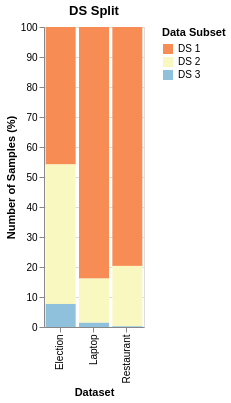
\includegraphics[scale=0.6]{images/augmentation/error_analysis/DS.png}
        }{
          \caption{Percentage of samples per \textit{DS} data subset.}
          \label{fig:aug_error_analysis_ds}
        }
        \capbtabbox{
          \begin{tabular}{|c|c|c|c|}
\hline
        & \multicolumn{3}{c|}{Data Subset} \\
\hline
Dataset &  DS 1 &  DS 2 &  DS 3 \\
\hline
Election   &  1164 &  1182 &   195 \\
\hline
Laptop     &   535 &    94 &     9 \\
\hline
Restaurant &   892 &   225 &     3 \\
\hline
\end{tabular}
        }{
          \caption{Number of samples within each \textit{DS} data subset.}
          \label{table:aug_error_analysis_ds}
        }
    \end{floatrow}
\end{figure}

The \textit{NT} split, unlike the \textit{DS} split, has a continuous number of subsets as $i$ of $NT_i$ is determined by the dataset. Figure \ref{fig:aug_error_analysis_nt_continuous} shows unsurprisingly that the Election dataset compared to the other two contains far fewer samples that only have one or two targets per text, which most likely relates to the fact that it has far fewer $DS_1$ samples. Thus, showing again that the Election dataset is likely to be a more difficult dataset, as a greater number of the samples will contain sentiment that are linked through target interaction. 
\begin{figure}[h!]
    \begin{floatrow}
        \ffigbox{
          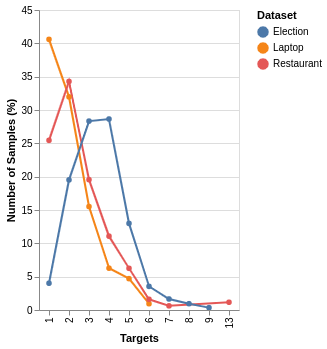
\includegraphics[scale=0.55]{images/augmentation/error_analysis/NT_continuous.png}
        }{
          \caption{Percentage of samples per $NT_i$ subset.}
          \label{fig:aug_error_analysis_nt_continuous}
        }
        \ffigbox{
          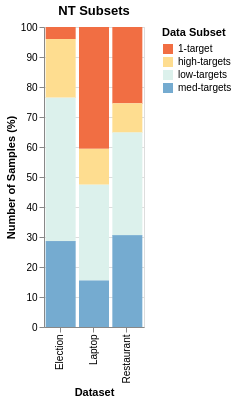
\includegraphics[scale=0.6]{images/augmentation/error_analysis/NT_discrete.png}
        }{
          \caption{Percentage of samples per \textit{NT} data subset.}
          \label{fig:aug_error_analysis_nt_discrete}
        }
    \end{floatrow}
\end{figure}
However, as can be seen in figure \ref{fig:aug_error_analysis_nt_continuous} and as stated in the work suggesting this split \citep{zhang-etal-2019-aspect} some of the subsets contain very few samples, thus any analysis on these subsets can be fairly unstable. Furthermore, as the dataset contains different ranges of $i$ in $NT_i$, binning the $NT$ split into four subsets will allow the datasets to be more comparable. The four subsets suggested would first be comprised of one subset where $i=1$ denoted. Then the other three subsets would be made up of low, medium, and high number of \textit{i}, where \textit{i} values for each of these subsets are based on the equal amount of samples per \textit{i}. Each of these subsets will be termed  \textit{1-target}, \textit{low-targets}, \textit{med-targets}, and \textit{high-targets} respectively. These subsets can be seen in figure \ref{fig:aug_error_analysis_nt_discrete} and table \ref{table:aug_error_analysis_nt}, along with the values of \textit{i} that each subset represents in table \ref{table:aug_error_analysis_nt_range}. The \textit{1-target} subset denotes the methods baseline performance when not having to consider target interaction, which to some extent should set the upper bound for all other subsets. The other three subsets represent low to high likelihood of requiring target interaction knowledge to classify the samples correctly. Thus, a method that can model these interactions well should perform well across all four subsets, whereas a method that cannot will perform increasingly better from high \textit{i} to $i=1$.
\begin{table}[!ht]
    \centering
    \begin{tabular}{|c|c|c|c|c|}
\hline
        & \multicolumn{4}{c|}{Data Subset} \\
\hline
Dataset &  1-target &  low-targets &   med-targets &   high-targets \\
\hline
Election   &       102 &        1216    &          728 &           495 \\
\hline
Laptop     &       259 &        204     &           99 &            76 \\
\hline
Restaurant &       285 &        384    &           343 &           108 \\
\hline
\end{tabular}
    \caption{Number of samples per \textit{NT} subset.}
    \label{table:aug_error_analysis_nt}
\end{table}

\begin{table}[!ht]
    \centering
    \begin{tabular}{|c|c|c|c|c|}
\hline
        & \multicolumn{4}{c|}{Data Subset} \\
\hline
Dataset &  1-target & low-targets  & med-targets & high-targets \\
\hline
Election   &  1, 1 &     2, 3  & 4, 4  &   5, 9 \\
\hline
Laptop     &  1, 1 &    2, 2  &     3, 3 &     4, 6 \\
\hline
Restaurant &  1, 1 &    2, 2 &     3, 4 &     5, 13 \\
\hline
\end{tabular}
    \caption{Range of \textit{i} values that represent each \textit{NT} subset.}
    \label{table:aug_error_analysis_nt_range}
\end{table}

The \textit{TSSR} split has a continuous number of subsets based on the dataset, of which the \textit{TSSR} subset values can range from $1$ to $0$. These \textit{TSSR} subsets can be seen in full in figure \ref{fig:aug_error_analysis_tssr_full} for each dataset. As noted before in section \ref{section:error_analysis_new_splits} the $1$ \textit{TSSR} subset is equal to the $DS_1$ subset of which this subset dominates the Laptop and Restaurant datasets. Thus for \textit{TSSR} value subsets less than $1$ the Laptop, Restaurant, and Election datasets contain $\sim20\%$, $\sim24\%$, and $\sim55\%$ of their samples respectively. Furthermore, it can be seen clearly from figure \ref{fig:aug_error_analysis_tssr_small} and \ref{fig:aug_error_analysis_tssr_full} that only the Election dataset has a large number of samples that have a \textit{TSSR} value less than or equal to $0.5$. These lower \textit{TSSR} values ($\leq 0.5$) represent the least or joint equal frequent sentiment within the text when the text comes from the $DS_2$ subset of which the majority of samples that contain more than one unique sentiment do come from the $DS_2$ for all datasets. Furthermore the lower \textit{TSSR} value subsets are going to be by far the more difficult samples to predict for, due to them containing targets that meet at least one of the two following criteria:
\begin{enumerate}
    \item The target coming from a text that contains lots of other targets but the target itself is within the least dominating sentiment class within the text.
    \item The target comes from a text that contains few targets but all targets come from a different sentiment class.
\end{enumerate}
Thus these two criteria therefore will measure the method's ability to identify target sentiment relations in a text that is dominated by other target sentiments.

\begin{figure}[!ht]
    \centering
    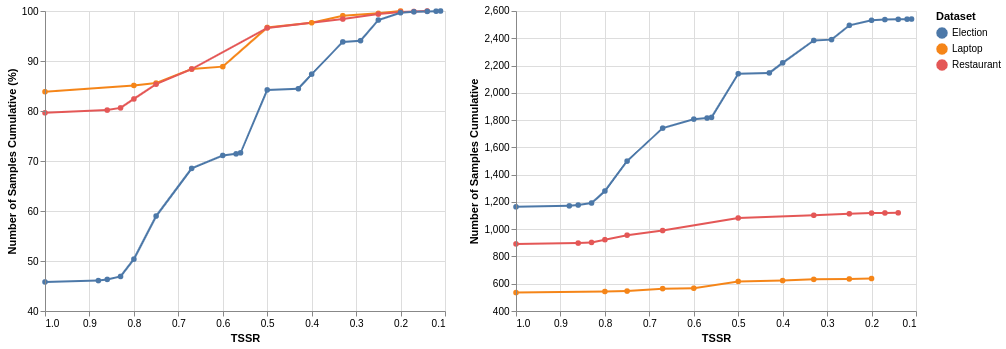
\includegraphics[scale=0.4]{images/augmentation/error_analysis/tssr_full_range.png}
    \caption{The right (left) plot shows the cumulative sample count (percentage) for decreasing values of \textit{TSSR}.}
    \label{fig:aug_error_analysis_tssr_full}
\end{figure}

\begin{figure}[!ht]
    \centering
    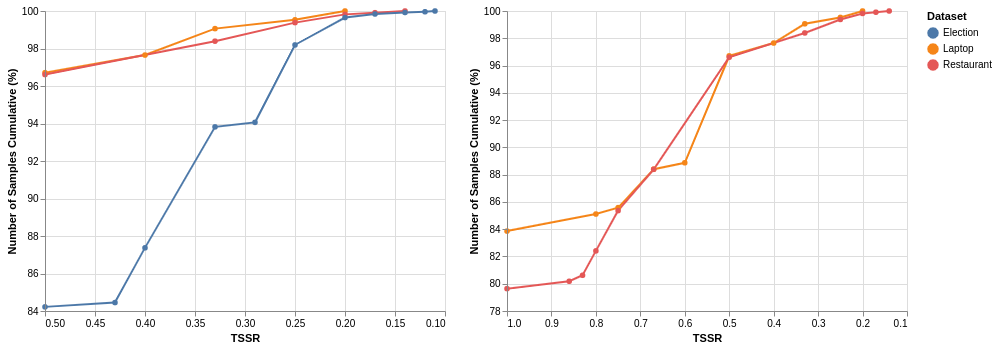
\includegraphics[scale=0.4]{images/augmentation/error_analysis/tssr_small_range.png}
    \caption{The left plot shows the cumulative sample count percentage for decreasing values of \textit{TSSR} starting from $0.5$. The right plot shows the same as the left but for the full range of \textit{TSSR} values but excluding the Election dataset.}
    \label{fig:aug_error_analysis_tssr_small}
\end{figure}

As can be seen from the figures of \ref{fig:aug_error_analysis_tssr_small} and \ref{fig:aug_error_analysis_tssr_full} the \textit{TSSR} value subsets are different depending on the dataset just like the \textit{NT} split. Therefore, the split will contain four subsets to represent different levels of difficulty and allow the performance on the subsets to be comparable across datasets. The four subsets are the following:

\begin{enumerate}
    \item \textit{1-TSSR} contains all targets that come from a sentence that only contain that one target thus this is the same as the $NT_1$/\textit{NT 1-target} subset and \textit{ST1} subset from section \ref{section:aug_error_analysis_previous_work}. 
    \item \textit{1-multi-TSSR} contains all targets that come from a sentence that contains more than one target but they all have the same sentiment value. This is the same as the difference of the $DS_1$ subset and the $NT_1$/\textit{NT 1-target} subset, and the same as the \textit{ST2} subset from section \ref{section:aug_error_analysis_previous_work}.
    \item \textit{high-TSSR} contains all of the targets that are within the following \textit{TSSR} value range $m \le x < 1$. 
    \item \textit{low-TSSR} contains all of the targets that are within the following \textit{TSSR} value range $0 \le x < m$.
\end{enumerate}

The value for $m$ is dataset specific and is based on ensuring that the \textit{low-TSSR} values contain at least 50\% of the samples after the \textit{1-TSSR} and \textit{1-multi-TSSR} samples have been removed from the dataset. The rest of the samples are given to the \textit{high-TSSR} subset. 

The \textit{1-TSSR} subset explores the effect of having no target interaction nor complex target sentiment relation due to only having one target and one sentiment. The \textit{1-multi-TSSR} explores the effect of having target interaction with potentially easier target sentiment relation due to the targets having all of the same sentiment, thus allowing the method to get the target sentiment relation incorrect without any consequence. The \textit{high-TSSR} and \textit{low-TSSR} measures the effect of increasing the target interaction and target sentiment relation to a smaller and larger degree respectively. 

The \textit{1-multi-TSSR} is expected to be the easiest subset as a method can make use of the target interaction and incorrectly inferring the correct target sentiment relationships as all targets will have the same sentiment. The next easiest subset would be the \textit{1-TSSR} due to no target interaction nor complex target sentiment relationships, however more difficult than \textit{1-multi-TSSR} as the method will have less sentiment signal within the text. Lastly the \textit{high-TSSR} and then \textit{low-TSSR} should be the most difficult subsets in that order due to target interactions and complex target-sentiment relationships. Furthermore, as stated earlier in section \ref{section:error_analysis_new_splits} the main purpose of this split is to measure overfitting to most frequent sentiment within the text. Through the subsets the overfitting could be detected if the method performs better in the \textit{1-multi-TSSR} than the \textit{1-TSSR}, this could show that either the method is exploiting the frequent sentiment situation or it is better at capturing the target interaction. However, the difference in performance between the \textit{high-TSSR} and \textit{low-TSSR} could detect this overfitting better due to the \textit{low-TSSR} coming from the most infrequent sentiment within the texts and the \textit{high-TSSR} coming from the most frequent. Thus if the difference between the \textit{high-TSSR} and the \textit{low-TSSR} is large then most frequent sentiment overfitting is more than likely occurring.

Within figure \ref{fig:aug_error_analysis_tssr_subsets} and table \ref{table:aug_error_analysis_tssr_subsets} is the breakdown of the number of samples per \textit{TSSR} subset, table \ref{table:aug_error_analysis_tssr_subsets_range} shows the \textit{TSSR} value range for each subset\footnote{\textit{1-multi-TSSR} is not within this table as it has the same range as \textit{1-TSSR}.} (the gap in range between each subset exists because there are no samples that contain a \textit{TSSR} value in that gap). As shown in the figure and tables, the Election dataset compared to the other two contains far fewer \textit{1-TSSR} samples compared to the number of samples in \textit{1-multi-TSSR}. Furthermore, the Election dataset also contains a large \textit{high-TSSR} subset, and low compared to the other datasets. 

\begin{figure}[!ht]
    \centering
    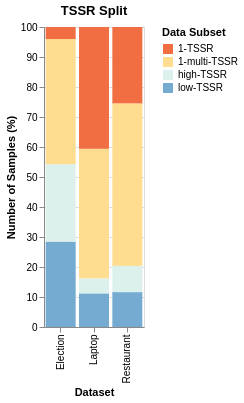
\includegraphics[scale=0.6]{images/augmentation/error_analysis/tssr_subsets.png}
    \caption{Percentage of samples per \textit{TSSR} subset.}
    \label{fig:aug_error_analysis_tssr_subsets}
\end{figure}

\begin{table}[!ht]
    \centering
    \begin{tabular}{|c|c|c|c|c|}
\hline
            &  \multicolumn{4}{c|}{Data Subset} \\
\hline 
Dataset &  1-TSSR &  1-multi-TSSR &  high-TSSR &  low-TSSR \\ 
\hline
Election   &     102 &          1062 &        656 &       721 \\
\hline  
Laptop     &     259 &           276 &         32 &        71 \\
\hline  
Restaurant &     285 &           607 &         98 &       130 \\
\hline 
\end{tabular}
    \caption{Number of samples within each \textit{TSSR} subset.}
    \label{table:aug_error_analysis_tssr_subsets}
\end{table}

\begin{table}[!ht]
    \centering
    \begin{tabular}{|c|c|c|c|}
\hline
            &  \multicolumn{3}{c|}{Data Subset} \\
\hline 
Dataset &  1-TSSR &   high-TSSR &  low-TSSR \\ 
\hline
Election   &     1, 1 &        0.88, 0.56 &       0.5, 0.11 \\
\hline  
Laptop     &     1, 1 &         0.8, 0.6 &        0.5, 0.2 \\
\hline  
Restaurant &     1, 1 &         0.86, 0.67 &       0.5, 0.14 \\
\hline 
\end{tabular}
    \caption{Range of \textit{TSSR} values for each \textit{TSSR} subset.}
    \label{table:aug_error_analysis_tssr_subsets_range}
\end{table}

To further understand the relationship between the \textit{TSSR} split and the \textit{NT} and \textit{DS} splits figure \ref{fig:aug_error_analysis_tssr_ds_nt_breakdown} shows the breakdown of each \textit{TSSR} subset by the \textit{NT} and \textit{DS} splits. As can be seen from the figure for the \textit{1-multi-TSSR} subset, the Election dataset has a more even distribution of samples that come from sentences that contain 2, 3, and 4 targets. Compared to the Restaurant and Laptop datasets where the majority of samples contain only 2 targets and then dramatically decreases as \textit{NT} increases. For all datasets the \textit{high-TSSR} subset contains relatively more samples that come from texts that contain a larger number of targets compared to the \textit{low-TSSR} subset. This is most likely due to the fact that targets with rare sentiment within the target's sentence only occur once or twice in a large \textit{NT} sentence where as the lesser rare sentiment targets occur far more often in those sentences and are counted within the \textit{high-TSSR} subset. An example of this can be thought of where the sentence contains 5 targets of which 1 comes from the positive sentiment class and the rest negative, thus the \textit{high-TSSR} will have 4 samples where as the \textit{low-TSSR} only 1 from the sentence coming from the 5 \textit{NT} subset. Unsurprisingly the majority of the limited number of $DS_3$ samples are almost all inclusively within the \textit{low-TSSR} subset for all datasets. Figure \ref{fig:aug_error_analysis_tssr_ds_nt_breakdown} also shows that the main difference between the three subsets is less about the distribution of \textit{NT} but rather the distribution of sentiment labels within a sentence. Lastly, figure \ref{fig:aug_error_analysis_tssr_ds_nt_breakdown} explains to some degree the reason why Election and Restaurant datasets have a large \textit{TSSR} value range as shown in table \ref{table:aug_error_analysis_tssr_subsets_range}, as these datasets must contain sentences that have a large number of targets as well as those sentences containing a different number of sentiments. 

\begin{figure}[!ht]
    \centering
    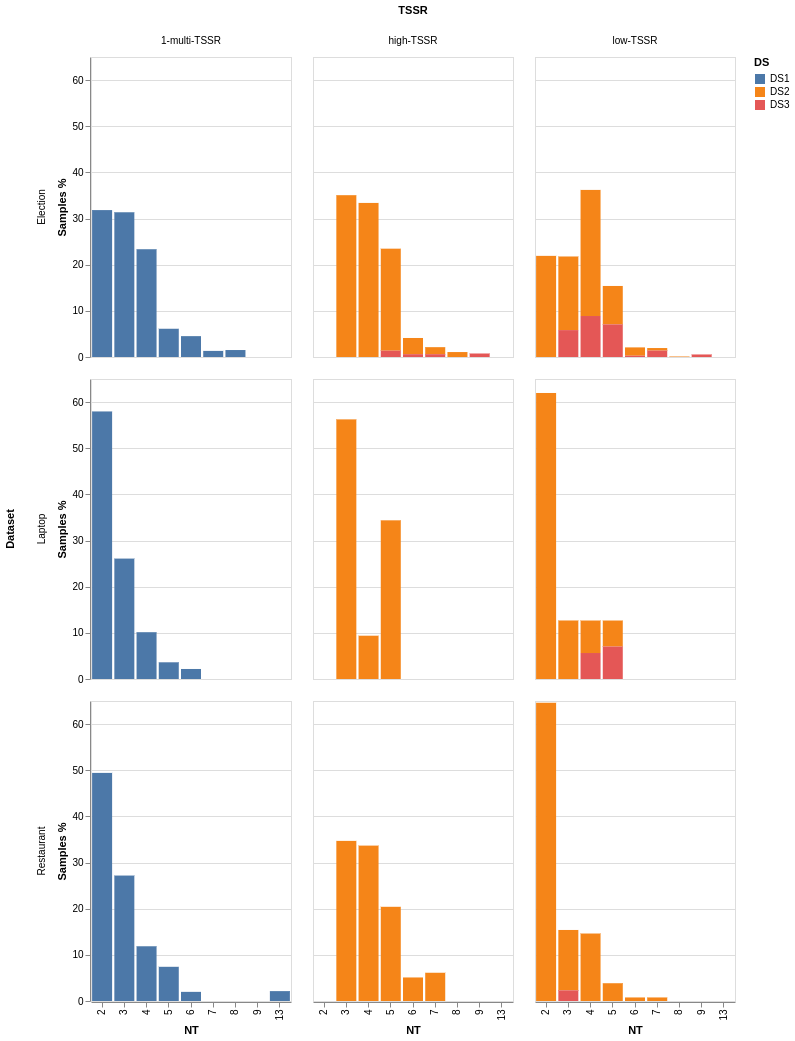
\includegraphics[scale=0.51]{images/augmentation/error_analysis/tssr_nt_ds.png}
    \caption{Percentage of samples per \textit{TSSR} subset broken down by \textit{NT} and \textit{DS} splits.}
    \label{fig:aug_error_analysis_tssr_ds_nt_breakdown}
\end{figure}

Similar to \textit{NT}, and \textit{TSSR} the \textit{n-shot} split has different values of \textit{n} based on the dataset, of which this can be best seen in figure \ref{fig:aug_n_shot_cuml}. From the left plot in figure \ref{fig:aug_n_shot_cuml} the sharpness of each curve for each dataset would appear to relate to the size of the dataset, as Laptop is the smallest and has the sharpest curve, whereas Election is the largest and has the least steep curve. Furthermore, in the left plot it can be seen that both Restaurant and Election start to flatten off around 80\% and 64\% suggesting that the test dataset contains a lot of samples with targets that have been very frequently seen in the training dataset. Thus these high \textit{n} samples should be easy to classify due to the method having seen lots of samples of those targets in the training dataset. To better capture how many samples with no target in training data appear compared to those with targets that appear very often, figure \ref{fig:aug_n_shot_low_med_high} contains three plots showing the low, medium, and high frequencies of \textit{n} (note that the values on the Y-axis are different). From this we can clearly see that for all datasets the largest number of samples occurs when $n=0$. Lastly, it shows that both the Restaurant and Election datasets contain a lot of samples where the targets have been seen very frequently in the training dataset.

\begin{figure}[h!]
    \centering
    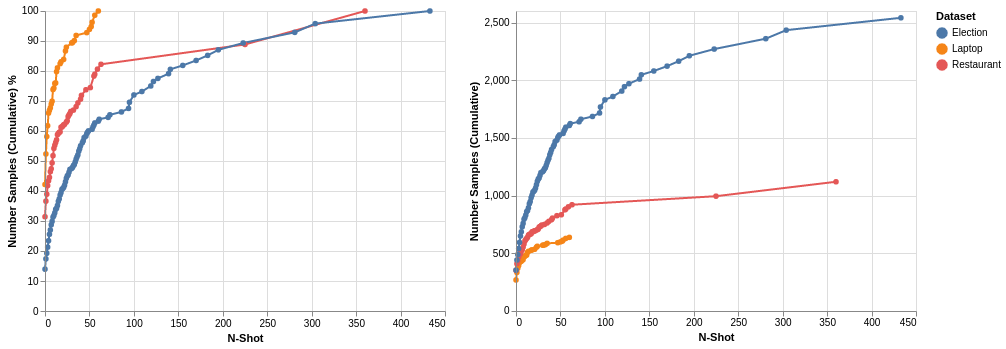
\includegraphics[scale=0.4]{images/augmentation/error_analysis/n_shot_cuml.png}
    \caption{The right (left) plot shows the cumulative sample count (percentage) for increasing values of \textit{n}.}
    \label{fig:aug_n_shot_cuml}
\end{figure}

This analysis suggests that the \textit{n-shot} split should be broken up into four different subsets rather than \textit{n} subsets, similar to the \textit{NT} split. This is suggested as a comparison of \textit{n} subsets with respect to some metric can be very unstable as some of these \textit{n} subsets can contain very few samples e.g. when $n=12$ for the Laptop dataset (see figure \ref{fig:aug_n_shot_low_med_high}). The four subsets suggested would first comprise of one subset where $n=0$ which is the \textit{UT} and \textit{zero-shot} case. Then the other three subsets would be made up of low, medium, and high number of \textit{n}, where \textit{n} values for each of these subsets are based on the equal amount of samples per \textit{n}. Each of these subsets will be termed \textit{zero-shot}, \textit{low-shot}, \textit{med-shot}, and \textit{high-shot} respectively. These subsets can be seen in figure \ref{fig:aug_error_analysis_n_shot_discrete} and table \ref{table:aug_error_analysis_n_shot}, along with the values of \textit{n} that each subset represents in table \ref{table:aug_error_analysis_n_shot_n_relation}. Lastly these subsets should allow for comparability across datasets and better analysis of the method's ability of learning a new target, as a good method should have a steady high performance across all of these subsets, whereas a method that overfits to targets would have a decreasing performance from the high to zero shot subsets.

\begin{figure}[!ht]
    \centering
    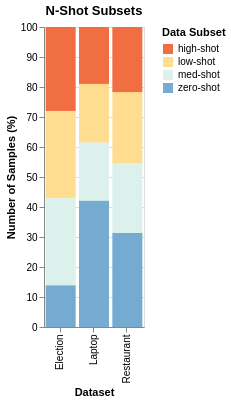
\includegraphics[scale=0.6]{images/augmentation/error_analysis/n_shot_discrete.png}
    \caption{Percentage of samples per \textit{n-shot} data subset.}
    \label{fig:aug_error_analysis_n_shot_discrete}
\end{figure}

\begin{table}[ht!]
    \centering
    \begin{tabular}{|c|c|c|c|c|}
\hline
        & \multicolumn{4}{c|}{Data Subset} \\
\hline
Dataset &   zero-shot &  low-shot &  med-shot &  high-shot \\
\hline
Election   &        354 &       740 &       736 &         711 \\
\hline
Laptop     &        269 &       125 &       123 &         121 \\
\hline
Restaurant &        352 &       267 &       258 &         243 \\ 
\hline
\end{tabular}
    \caption{Number of samples per \textit{n-shot} subset.}
    \label{table:aug_error_analysis_n_shot}
\end{table}

\begin{table}[ht!]
    \centering
    \begin{tabular}{|c|c|c|c|c|}
\hline
        & \multicolumn{4}{c|}{Data Subset} \\
\hline
Dataset &     zero-shot &   low-shot &     med-shot &  high-shot \\
\hline
Election   &  0, 0 &  1, 23 &  24, 100 &   109, 433 \\
\hline
Laptop     &    0, 0 &   1, 3 &    4, 14 &   17, 60 \\
\hline
Restaurant &    0, 0 &  1, 11 &   12, 55 &   56, 360 \\
\hline
\end{tabular}
    \caption{Range of \textit{n} values that represent each \textit{n-shot} subset.}
    \label{table:aug_error_analysis_n_shot_n_relation}
\end{table}

\begin{sidewaysfigure}[!ht]
    \centering
    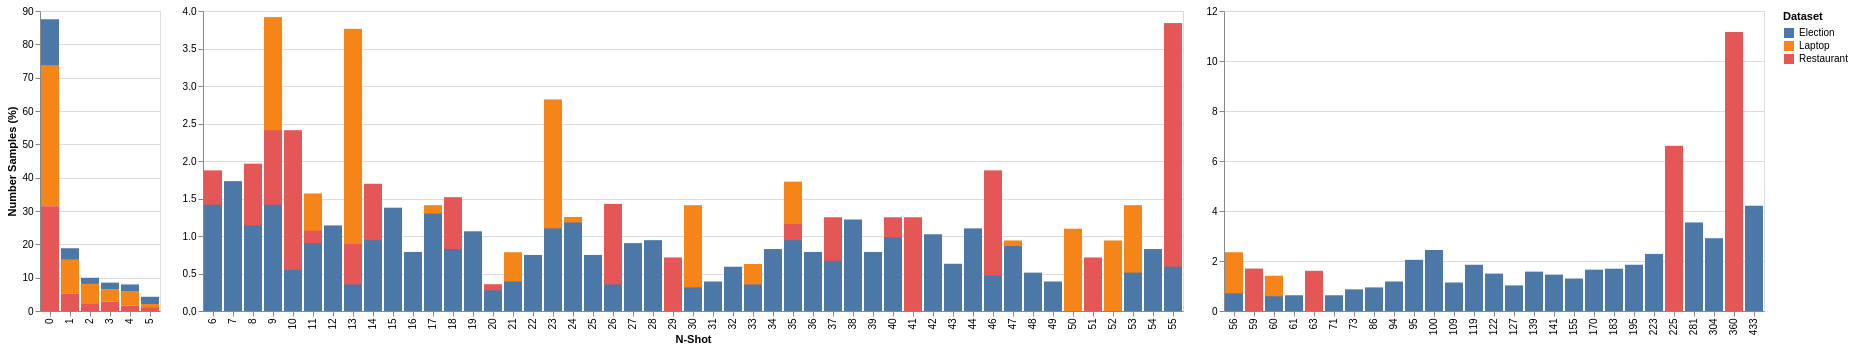
\includegraphics[scale=0.3]{images/augmentation/error_analysis/n_shot_low_med_high.png}
    \caption{Number of samples as a percentage per value of \textit{n}.}
    \label{fig:aug_n_shot_low_med_high}
\end{sidewaysfigure}

\textit{TRS}, the last and new split to be analysed can be best seen through figure \ref{fig:aug_error_analysis_trs} and table \ref{table:aug_error_analysis_trs}. As can be seen the \textit{UT} subset is almost the largest subset for the smallest dataset (Laptop) but a relatively small subset for the largest dataset, of which this has already been seen through the \textit{zero-shot} subset. Furthermore, the \textit{USKT} is the smallest subset by far across the datasets, however it still counts for at least 10\% of all data in the Laptop dataset. Based on the two global splits, \textit{TRS} and \textit{n-shot}, they show the importance of a method to generalise to new targets (\textit{UT} and \textit{zero-shot} cases) and new relations (\textit{USKT}) which will more likely occur in a low resource setting, which can be best seen by the size of these subsets on the Laptop dataset. 

\begin{figure}[ht!]
    \begin{floatrow}
        \ffigbox{
          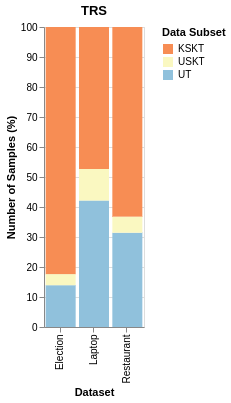
\includegraphics[scale=0.6]{images/augmentation/error_analysis/TRS.png}
        }{
          \caption{Percentage of samples per \textit{TRS} data subset.}
          \label{fig:aug_error_analysis_trs}
        }
        \capbtabbox{
          \begin{tabular}{|c|c|c|c|}
\hline
            &  \multicolumn{3}{c|}{Data Subset} \\
\hline
Dataset     &  KSKT &  USKT &  UT  \\
\hline
Election    & 2093  & 94    &  354 \\
\hline
Laptop      & 302   & 67    &  269 \\
\hline
Restaurant  & 708   & 60    &  352 \\
\hline
\end{tabular}
        }{
          \caption{Number of samples within each \textit{TRS} data subset.}
          \label{table:aug_error_analysis_trs}
        }
    \end{floatrow}
\end{figure}

\FloatBarrier
\subsection{Conclusion so far}
Within this subsection the different error splits that exist within the TDSA literature have been reviewed and added too. Furthermore, each of these splits have been analysed on three major datasets showing for the first time how each dataset has different characteristics. The local splits \textit{DS}, \textit{NT}, and \textit{TSSR} show that the Election dataset contains far more unique sentiments per text, whereas the Restaurant dataset contains the most targets per text. The global splits, \textit{n-shot} and \textit{TRS}, find that in the low resource setting a method that can generalise well to new targets and new sentiment relations would be important, which can be seen through the contrast in subset sizes between Election and Laptop datasets. Lastly, table \ref{table:aug_error_split_summary} summarises the differences in the error splits, examples for each of these splits and subsets can be found in table \ref{table:aug_error_split_examples}. Finally, a summary of all of the statistical breakdowns of each of these splits can be found in table \ref{table:aug_error_analysis_summary_stats}.

\begin{table}[!ht]
    \centering
    \begin{tabular}{|c|c|c|c|c|}
\hline
    &    & \multicolumn{3}{c|}{Dataset} \\
\hline
Data Split & Data Subset &  Election &  Laptop &  Restaurant \\
\hline
\multirow{3}{*}{$DS_i$} & $DS_1$ &      45.8\% &    83.9\% &        79.6\% \\
 & $DS_2$ &      46.5\% &    14.7\% &        20.1\% \\
 & $DS_3$ &       7.7\% &     1.4\% &         0.3\% \\
\hline
 \multirow{4}{*}{\textit{NT}} & \textit{1-target} &       4.0\% &    40.6\% &        25.4\% \\
 & \textit{low-targets} &      47.9\% &    32.0\% &        34.3\% \\
 & \textit{med-targets} &      28.7\% &    15.5\% &        30.6\% \\
 & \textit{high-targets} &      19.5\% &    11.9\% &         9.6\% \\
\hline
 \multirow{4}{*}{\textit{TSSR}} & \textit{1-TSSR} &       4.0\% &    40.6\% &        25.4\% \\
 & \textit{1-multi-TSSR} &      41.8\% &    43.3\% &        54.2\% \\
 & \textit{high-TSSR} &      25.8\% &    5.0\% &         8.8\% \\
 & \textit{low-TSSR} &      28.4\% &    11.1\% &        11.6\% \\
 \hline
 \multirow{3}{*}{\textit{TRS}} & \textit{KTKS} &      82.4\% &    47.3\% &        63.2\% \\
 & \textit{USKT} &       3.7\% &    10.5\% &         5.4\% \\
 & \textit{UT} &      13.9\% &    42.2\% &        31.4\% \\
\hline
 \multirow{4}{*}{\textit{n-shot}} & \textit{zero-shot} &      13.9\% &    42.2\% &        31.4\% \\
 & \textit{low-shot} &      29.1\% &    19.6\% &        23.8\% \\
 & \textit{med-shot} &      29.0\% &    19.3\% &        23.0\% \\
 & \textit{high-shot} &      28.0\% &    19.0\% &        21.7\% \\
\hline
 \multicolumn{2}{|c|}{Total Samples}           &    2541 &  638 &      1120 \\
\hline
 \end{tabular}
    \caption{Summary statistics of all splits}
    \label{table:aug_error_analysis_summary_stats}
\end{table}

\FloatBarrier
\section{Method Performance on the Error Splits}
\subsection{Introduction}
\label{section:aug_method_performance_intro}
In this sub-section the performance of the following four NN based methods will be analysed across the five different error splits stated in section \ref{section:aug_error_analysis}. The results from these experiments will be used to further analyse what the error splits show as well as create multiple baselines for these splits. The four different methods are the following: 
\begin{enumerate}
    \item \textit{CNN} -- The sentence level CNN from \citet{kim-2014-convolutional} that encodes the context/sentence and does not take into account the target.
    \item \textit{TDLSTM} \citep{tang-etal-2016-effective} -- An LSTM that encodes the target by ensuring the target word(s) are always the last word(s) fed to the LSTM from the context/sentence. Thus a position based method where the position is encoded through the NN architecture. This is the same TDLSTM as that from chapter \ref{chapter:reproducibility}, described in detailed within section \ref{section:repro_lstm_description}.
    \item \textit{IAN} \citep{ma2017interactive} -- Encodes the target into the context via attention.
    \item \textit{Att-AE} -- A model that is the same as the \textit{AE} model from \citet{wang-etal-2016-attention} but with an attention layer after the LSTM enocder. This model is also the same as the inter-aspect model (from now on called \textit{Inter-AE}) from \citet{hazarika-etal-2018-modeling} but without the LSTM aspect encoder (phase 2 in figure 1) that models other targets from the same context/sentence.  
\end{enumerate}
Thus to summarise the differences in the TDSA methods (last three methods from above); \textit{TDLSTM} encodes the position of targets through its architecture, \textit{IAN} encodes the target into the context via attention and also encodes the context into the target through attention, and \textit{Att-AE} encodes the target into the context through concatenation of the target vector onto each word vector within the context before the LSTM encoder. The \textit{Att-AE} does perform attention over the context but unlike \textit{IAN} does not explicitly model the target in the attention of the context nor does it perform attention over the target word(s)\footnote{For the detailed reader, the \textit{IAN's} attention can be denoted as \textit{general} where as \textit{Att-AE} would be \textit{concat} based on the notation from \citet[\S3.1]{luong-etal-2015-effective}.}.

%Furthermore as stated in the introduction section \ref{section:aug_introduction}, the TDSA methods will be enhanced with three different developments; 1. position-encoding, 2. inter-target encoding, and 3. CWR. From the three methods, only \textit{IAN} and \textit{Att-AE} will be enhanced with position-encoding as \textit{TDLSTM} already has the target position somewhat encoded into its NN architecture. Each of these enhancements will be tested against their standard/base model with respect to the error analysis splits. The quantitative results from these error analysis splits will be compared to the original qualitative justifications for these developments from the respective papers.

The reason why \textit{Att-AE} is neither exactly \textit{AE} \citep{wang-etal-2016-attention} nor \textit{Inter-AE} \citep{hazarika-etal-2018-modeling} is due to not wanting to add inter-target encoding to the baseline models, as within chapter \ref{chapter:case_study_methodology} all models are going to have inter-target encoding added. Furthermore as the model will have inter-target encoding added in chapter \ref{chapter:case_study_methodology} it will convert \textit{Att-AE} to \textit{Inter-AE} thus making it a standard model from prior literature. The use of different methods from those within chapter \ref{chapter:reproducibility} is due to the surge in purely NN based TDSA methods of recent years, thus the only methods used within this chapter are NN based.

Due to having a non-target method \textit{CNN}, all of the TDSA methods have a baseline to compare against. Furthermore as all experiments will contain results from at least two TDSA methods to a larger extent the results should generalise to different TDSA NN architectures. In the following sections the thesis will:
\begin{enumerate}
    \item State the experimental setup of all experiments within this section (section \ref{section:aug_experimental_setup}).
    \item Explore the differences in performance on the error splits across the methods (section \ref{section:aug_baseline}).
    %\item Evaluate the error split across three different model enhancements position encoding (section \ref{section:aug_position_encoding}), inter target encoding (section \ref{section:aug_inter_target_encoding}), and CWR (section \ref{section:aug_cwr}).
\end{enumerate}

\FloatBarrier
\subsection[Experimental Setup]{Experimental Setup\footnote{The code to generate table \ref{table:aug_methods_performance_split_breakdown} can be found in the README at the following \url{https://github.com/apmoore1/tdsa_comparisons\#analysis-of-the-datasets}. The code to generate tables \ref{table:aug_methods_performance_global_error_diff} and \ref{table:aug_methods_performance_local_error_diff} can be found in the following notebook \url{https://github.com/apmoore1/tdsa_comparisons/blob/master/analysis/TDSA_Error_Analysis.ipynb}.}}
\label{section:aug_experimental_setup}
As stated in the introductory section of this chapter (\ref{section:aug_introduction}), the three datasets that are used throughout this chapter are the Election, Laptop and Restaurant datasets. However, unlike the error analysis section (\ref{section:aug_error_analysis}), the standard training split for each of the datasets will be further randomly split into a new training and an additional validation split, of which the size of these splits can be seen in table \ref{table:aug_methods_performance_split_breakdown}. The validation set is required so that the early stopping can be used for all of the NN methods. Furthermore, the validation set would usually be used for more hyper-parameter tuning, e.g. finding the best learning rate etc, but due to compute time this is not the case. Instead we selected the most common hyper-parameters from the literature as detailed in table \ref{table:aug_methods_performance_default_hyperparameters}, it will be stated explicitly within this chapter if these hyperparameters are not used. One default hyperparameter of note is the embedding, of which the 840 billion token 300 dimensional GloVe vector \citep{pennington-etal-2014-glove} (from now on called GloVe and is called that in table \ref{table:aug_methods_performance_default_hyperparameters})\footnote{This is the same 300 dimension GloVe embedding that is used in chapter \ref{chapter:reproducibility}.} was chosen, as it is the most common default embedding in the TDSA literature. All text will be tokenised using Spacy and then lower-cased\footnote{The text was lower-cased as none of the three TDSA methods stated in their original works if they lower-cased the text's or not. The assumption here is that they did.}. Lastly, all results reported in this section will be results on the test set and all validation results will be reported in the appendix for reproducibility reasons \citep{dodge-etal-2019-show}. However if there is a large difference between the validation and test results this will be mentioned explicitly in this section.

\begin{table}[h!]
    \centering
    \begin{tabular}{|c|c|c|c|c|}
\hline
        & \multicolumn{4}{c|}{Data Split} \\
\hline
Dataset &          Train &     Validation &           Test &  Total \\
\hline
Election   &  6811 (57.24\%) &  2547 (21.41\%) &  2541 (21.35\%) &  11899 \\
\hline
Laptop     &  1661 (56.29\%) &   652 (22.09\%) &   638 (21.62\%) &   2951 \\
\hline
Restaurant &  2490 (52.73\%) &  1112 (23.55\%) &  1120 (23.72\%) &   4722 \\
\hline
\end{tabular}
    \caption{Number of samples.}
    \label{table:aug_methods_performance_split_breakdown}
\end{table}

Due to the splitting of the training dataset, the error analysis split statistics in section \ref{section:aug_error_analysis} will not be identical for the global error splits (\textit{n-shot} and \textit{TRS}) between the train/test and train/validation as they rely on a comparison of train and validation/test. Even though they will not be identical they are relatively similar as shown by table \ref{table:aug_methods_performance_global_error_diff}. Furthermore, as the local splits (\textit{DS}, \textit{NT}, and \textit{TSSR}) are only reported for the test set, table \ref{table:aug_methods_performance_local_error_diff} shows them for the validation and test set showing that they are again relatively similar, thus results should be comparable between validation and test sets.

Furthermore, for all of the experiments performed in this chapter each model will have trained/ran on the respective data eight times. Thus allowing for the random seed problem, that is known in NN methods within NLP \citep{reimers-gurevych-2017-reporting}, and to be able to perform statistical significance tests that take into account this problem \citep{reimers2018comparing}\footnote{These significance tests are different to those used in chapter \ref{chapter:reproducibility}, as these for the neural network based methods better take into account all runs produced by different random seeds.}. \citet{reimers2018comparing} has shown that by using a minimum of eight runs two models can be compared with a confidence level of 99\% which is equivalent to $p \leq 0.01$ no matter if the scores from those runs comes from a non-normal distribution. The two scoring metrics commonly used in TDSA and will be used in this chapter are accuracy and macro F1, of which only accuracy can be assumed to produce scores originating from a normal distribution and thus can use the more powerful parametric tests \citep{dror-etal-2018-hitchhikers}. Therefore following \citet{reimers2018comparing} for the accuracy scores the significance test used will be the Welch's t-test (parametric test) \citep{welch1947generalization} and for macro F1 the Wilcoxon signed-rank test (non-parametric test) \citep{wilcoxon1992individual}. When comparing two models using these statistical tests for each test the one-tailed version of it will be used as in these experiments the requirement is only to know if one model is better than another. In this and the next chapter \ref{chapter:case_study_methodology}, a method is defined as the general NN architecture where as the model is defined as the concrete configuration of that method. Thus two models can be different but use the same method, for example the difference would be the word vectors that the two models use. When comparing two models across multiple variables and therefore significance tests a correction procedure is required, as explained in section \ref{section:repro_neural_pooling}. In this chapter, the Bonferroni correction procedure will be used where appropriate as in none of our cases can independence be assumed.

%Before going into the details of comparing two models across multiple variables, we first need to define what the differences are between a method and a model. A method is the general NN architecture where as the model is the concrete configuration of that method. Thus two models can be different but use the same method, for example the difference would be the word vectors that the two models use. When comparing two model across multiple variables and therefore significance tests a correct procedure is required, as explained in section \ref{section:repro_neural_pooling}. In this chapter, Bonferroni correction procedure will be used where appropriate as in none of our cases can independence be assumed.   %When comparing two models the value of $\alpha$ in $p \leq \alpha$ is used to define the number of type 1 errors in the statistical test. However when comparing two models across multiple variables and therefore multiple significance tests if the number of times a test is defined as significant are simply counted the number of type 1 errors in the tests will increase \citep{dror-etal-2017-replicability}. Thus simply counting the number of times a test is significant cannot be used without further introducing type 1 errors. To bound these type 1 errors across multiple tests requires a correction mechanism of which \citet{dror-etal-2017-replicability} recommends Bonferroni (Fisher) when the variables are dependent (independent), where Fisher is the more powerful version. In this chapter, Bonferroni will be used where appropriate as in none of our cases can independence be assumed.

\FloatBarrier
\subsection[Baseline Results]{Baseline Results\footnote{All tables and graphs within this section have been generated through the following notebook \url{https://github.com/apmoore1/tdsa_comparisons/blob/master/analysis/TDSA_Baseline_Results.ipynb}. The exception to this are the tables generated within appendix \ref{section:appendix_cnn_tdsa_baseline}, of which there is a pointer in that appendix to the relevant notebook.}}
\label{section:aug_baseline}
\subsubsection{Introduction}
The baseline results use the four different methods stated in section \ref{section:aug_method_performance_intro} as is without any changes to their respective NN architectures. These results will be explored to see whether the intuition behind the error splits as stated in section \ref{section:aug_analysing_the_splits} is to a degree true. 

For clarification, the sentence/text level \textit{CNN} method is trained differently to the TDSA methods due to the fact that it does not model the target within the sentence. Thus instead of training the \textit{CNN} method with potentially the same sentence multiple times with potentially multiple different sentiments as is the case with TDSA datasets\footnote{This was how the non-target aware models from chapter \ref{chapter:reproducibility} were trained. Therefore the non-target aware models in some training samples would have been given the same sentence with different sentiments to train on. Even though it may have been better to train them in the ways stated within this section, this was not tested due to compute time. Furthermore it was assumed that they were trained in the same way as their target aware methods as it was not stated in the papers \citep{vo2015target, tang-etal-2016-effective, wang-etal-2017-tdparse} that were reproduced that they were trained any differently.}, the TDSA dataset is converted to a text level dataset. To convert from TDSA to a text dataset each text/sentence can only contain one sentiment, from this two options are plausible; 1. only uses texts that contain one unique sentiment ($DS_1$ dataset), or 2. use the majority sentiment from the text. These two options were compared of which the detailed results can be found in appendix \ref{section:appendix_cnn_tdsa_baseline}, of which it was found that the second/later option performed best on 2 of the 3 datasets and all datasets for the accuracy and macro f1 metrics respectively across both validation and test splits. For clarification, when predicting with this text level classification method all targets within the same text will be given the predicted text level sentiment label. This experiment of comparing the two options of training a text classifier on TDSA data was required as prior works that have shown results for text classifiers never explain how they were trained \citep{tang-etal-2016-aspect,wang-etal-2016-attention,he-etal-2018-exploiting,jiang-etal-2019-challenge}. For a stronger text classifier baseline one could consider pre-training the text classifier from large sources of annotated data such as Yelp reviews \citep{tang-etal-2015-learning}, Amazon reviews \citep{mcauley2015image,he2016ups}, or Tweets using distant supervision \citep{go2009twitter} for the Restaurant, Laptop, and Election datasets respectively and then fine tune them on the respective TDSA dataset. However this stronger baseline is not considered in this work as we are not looking at transfer learning from other sources of sentiment, but this has been shown to be beneficial for TDSA methods \citep{he-etal-2018-exploiting}.  

\FloatBarrier
\subsubsection{Overall Results}
Figure \ref{fig:aug_baseline_overall_scores} shows the results of the baseline models across both the validation and test splits with the associated tables \ref{table:aug_methods_baseline_tdsa_metrics_validation} and \ref{table:aug_methods_baseline_tdsa_metrics_test} in appendix \ref{appendix_augmentation_tables}. From these results it can be seen that the \textit{CNN} text classification baseline is indeed a strong baseline for the Laptop and Restaurant datasets that the TDSA methods find difficult to beat. 

\begin{figure}[ht!]
    \centering
    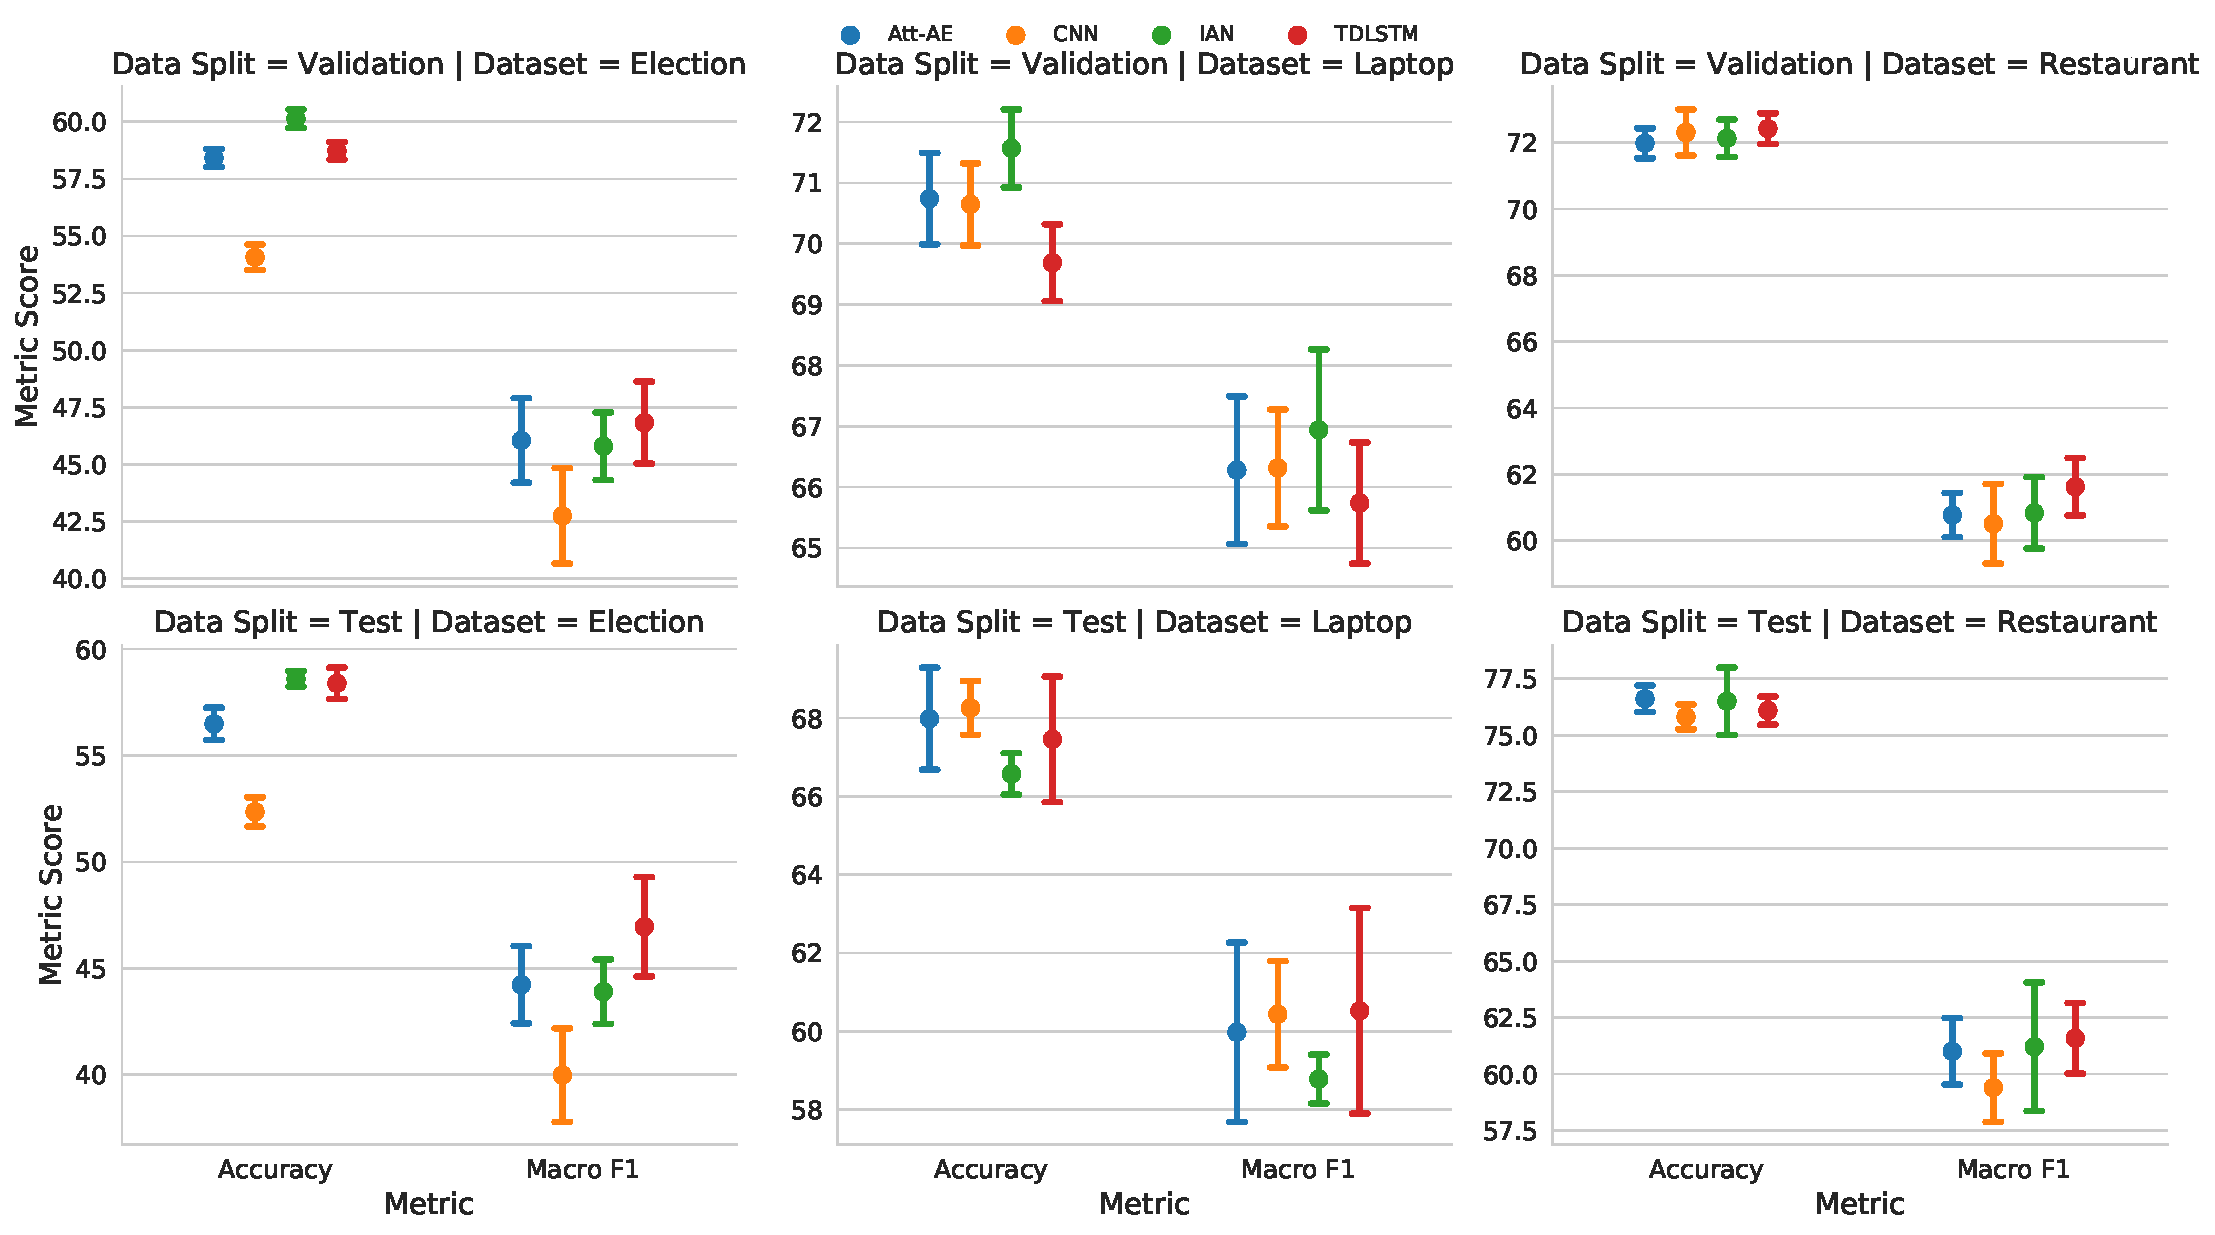
\includegraphics[scale=0.38]{images/augmentation/methods_performance/baseline/baseline_overall_scores.pdf}
    \caption{The mean and standard deviation error bars from running each model 8 times.}
    \label{fig:aug_baseline_overall_scores}
\end{figure}

\FloatBarrier
\subsubsection{Comparison of the Original Model Scores to the Reproduced Models}
Figure \ref{fig:aug_baseline_replication_scores} compares the single run performance of the original TDSA models scores from their associated papers to the distribution of eight accuracy scores from our reproduced TDSA methods\footnote{Accuracy metric was the only metric reported in all of the original TDSA method papers and none of them reported on the Election dataset.}. As can be seen from figure \ref{fig:aug_baseline_replication_scores} the models original score are within the distribution of scores from the reproduced models apart from \textit{IAN} where the original models performance is a lot higher especially for the Laptop dataset. \textit{IAN's} performance difference is most likely due to the fact that the reproduced version uses a different optimiser, ADAM \citep{kingma2014adam}, instead of SGD with momentum \citep{qian1999momentum}, this design choice was made so that all models used the same optimiser. Even though it would be good to optimise the performance of the \textit{IAN} model so that it produces scores similar to the original doing so in a fair manner would mean hyperparameter tuning the other models as well \citep{dodge-etal-2019-show}, which would start becoming computationally expensive. Thus in this thesis it is accepted that the \textit{IAN} model has not been reproduced to the same performance as the original paper reports.

\begin{figure}[ht!]
    \centering
    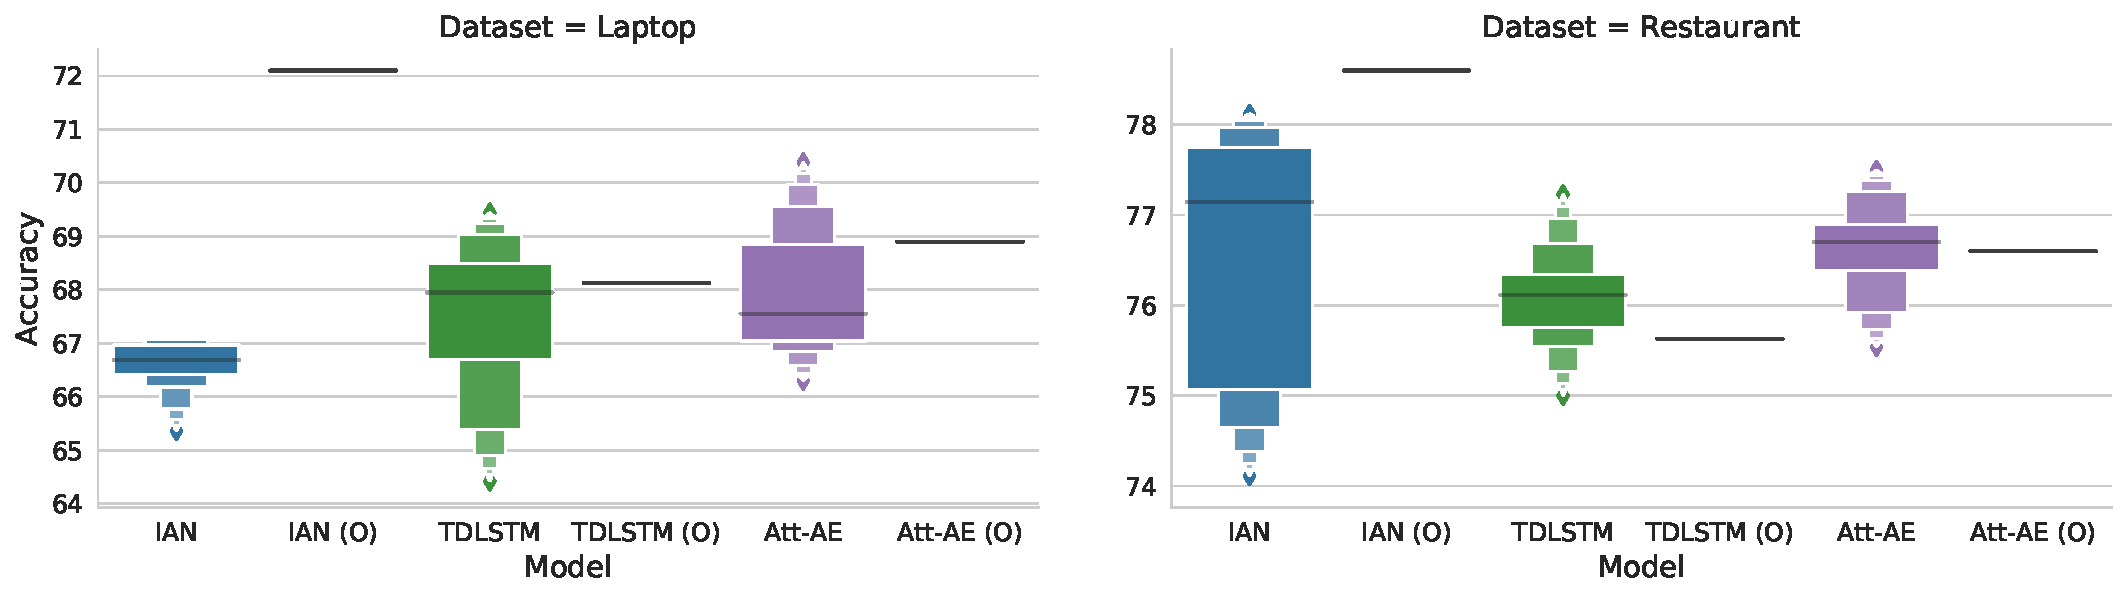
\includegraphics[scale=0.4]{images/augmentation/methods_performance/baseline/replication_experiment_baseline.pdf}
    \caption{Distribution of all scores and the line represents the mean value, of which for the original models this line represents their only reported score. Model names with a \textit{(O)} represent the score reported in the original models paper.}
    \label{fig:aug_baseline_replication_scores}
\end{figure}

\FloatBarrier
\subsubsection{Overall Results Comparison between TDSA and Text Classification Models}
This thesis shows for the first time that not all TDSA models are statistically significantly better than a text classifier as shown by table \ref{tab:augmentation_baseline_tdsa_text_classifier_p_values}, even though all three original TDSA papers state that their TDSA models are superior to a text classifier. Furthermore, at the $95\%$ confidence level none of the TDSA methods are significant on the Laptop test split no matter what the metric is. This shows that potentially hyperparameter tuning is very important to get the most out of the TDSA models. More likely the reason for the text classifier's strong performance on the Laptop and Restaurant dataset compared to the Election dataset is that these datasets contain a large quantity of $DS_1$ samples (see figure \ref{fig:aug_error_analysis_ds}), of which it is shown later in this section in figure \ref{fig:aug_baseline_test_error_subset} that the text classifier does at least as good if not better than the TDSA models on the $DS_1$ subset in the Laptop and Restaurant datasets. This further shows that the overall metrics tell us very little in what the difference is between a text classifier model and the TDSA models.  
%\citet{jiang-etal-2019-challenge} concluded as well for the Restaurant dataset\footnote{\citet{jiang-etal-2019-challenge} did not perform any significance tests between existing TDSA methods and the text classifier baselines.} that the text classifier good performance was due to the large quantity of text. Furthermore as shown 



\begin{table}[ht!]
    \centering
    \begin{tabular}{|c|c|c|c|c|c|}       
\hline
&            &  & \multicolumn{3}{c|}{Dataset} \\
\hline
Model & Split & Metric &      Election         &    Laptop       &  Restaurant           \\
\hline
Att-AE & \multirow{2}{*}{Test} & Accuracy &  \textbf{2.14e-08} &  0.68 &    \textbf{0.01} \\
&            & Macro F1 &  \textbf{7.86e-04} &  0.67 &    \textbf{0.03} \\
& \multirow{2}{*}{Validation} & Accuracy &  \textbf{2.57e-10} &  0.40 &    0.84 \\
&            & Macro F1 &  \textbf{3.76e-03} &  0.52 &    0.31 \\
\hline
IAN & \multirow{2}{*}{Test} & Accuracy &  \textbf{2.21e-10} &  0.99 &    0.14 \\
&            & Macro F1 &  \textbf{1.02e-03} &  0.99 &    0.08 \\
& \multirow{2}{*}{Validation} & Accuracy &  \textbf{3.98e-12} &  \textbf{0.01} &    0.69 \\
&            & Macro F1 &  \textbf{3.96e-03} &  0.16 &    0.30 \\
\hline
TDLSTM & \multirow{2}{*}{Test} & Accuracy &  \textbf{1.29e-10} &  0.87 &    0.19 \\
&            & Macro F1 &  \textbf{2.53e-05} &  0.46 &    \textbf{0.01} \\       
& \multirow{2}{*}{Validation} & Accuracy &  \textbf{1.26e-10} &  0.99 &    0.36 \\
&            & Macro F1 &  \textbf{8.07e-04} &  0.85 &    \textbf{0.03} \\
\hline
\end{tabular}
    \caption{The P-values for each model where the null hypothesis is that each model performs as well as a \textit{CNN} text classifier. The P-Values in bold are those $\leq 0.05$.}
    \label{tab:augmentation_baseline_tdsa_text_classifier_p_values}
\end{table}

\FloatBarrier
\subsubsection{Error Split Results}
\label{section:augmentation_cwr_error_split_results_sub}

The performance of all of the models across all datasets for each split and their associated subsets can be seen in figure \ref{fig:aug_baseline_test_error_subset} (appendix \ref{appendix_augmentation_figures} figure \ref{fig:aug_baseline_validation_error_subset} shows the validation split results). The figures that contain subset performance results will not contain results for the $DS_3$ subset for the Laptop and Restaurant datasets, this is due to the subset containing very few samples as highlighted in subsection \ref{section:aug_analysing_the_splits}. The error split results for the test and validation splits are better highlighted in figures \ref{fig:aug_baseline_test_error_diff_subset} and \ref{fig:aug_baseline_validation_error_diff_subset} respectively where the accuracy on the whole dataset (overall accuracy) is subtracted from the error subset accuracies. These figures can thus evaluate the error splits that were discussed and created within this section. In the list below the results will be analysed by error split:

\begin{itemize}
    \item \textit{DS} split, as expected, increases in difficulty as the number of unique sentiments in the text increases, thus showing that target sentiment relation to be a difficult task for the models to perform. Furthermore, it can be seen that on average the \textit{TDLSTM} model performs consistently well on the $DS_2$ and $DS_3$ subsets compared to the other models.
    \item \textit{NT} split does not have a consistent affect on the performance of the models, this was also found in one of the original papers \citep{zhang-etal-2019-aspect}. One would expect texts that contain a lot of targets to be more difficult and at times it is as shown by the Restaurant dataset. However, on the other two datasets this is not the case. Furthermore, the performance across the subsets can differ between datasets splits, e.g. the performance of all models on the \textit{med-targets} subset on the Election dataset is worse than \textit{high-targets} for all models on the test split, but on the validation figure (\ref{fig:aug_baseline_validation_error_diff_subset}) the opposite is true. This would suggest that even though theoretically a text with more targets should be more difficult for a model to classify, due to the complexities of matching targets to their respective sentiments \citep{zhang-etal-2019-aspect}, this is not the case. Thus later in this section, analysis is conducted to investigate what other factors are influencing the change in performance within the \textit{NT} split. However, for now it can be concluded that \textit{NT} cannot effectively evaluate the target interaction as no consistent trend can be found in this split.
    \item \textit{TSSR} As expected the \textit{1-Multi} subset is by far the easiest subset to classify suggesting that the models are exploiting the fact that all targets have the same sentiment. The \textit{1} subset tends to perform the next best with the \textit{high} subset at times quite close if not the same. A reason for the \textit{high} subset to have such high performance across the models could be due to the models overfitting to the most frequent sentiment class in the text, as suggested in section \ref{section:aug_error_analysis}. As expected the \textit{low} subset is by far the worst across all datasets and models and in some cases harder to classify than samples within $DS_2$ and $DS_3$. Only on the Laptop test split are the \textit{high} scores similar to the \textit{low}, of which this might be due to the lack of samples for the \textit{high} subset (5\% of the dataset) compared to the (11.1\% of the dataset) in the \textit{low} subset, which is also suggested by the large error bars. Furthermore the sentiment overfitting which this split is supposed to measure does show to some extent where the TDSA model, \textit{TDLSTM}, that performs consistently better or at least as good in the $DS_2$ and $DS_3$ subsets tends to have a smaller difference between subset \textit{1-Multi} and \textit{1}, and is consistently a lot higher than the text classifier on the \textit{low} subset. However this split does not measure sentiment overfitting explicitly very well without the text classification baseline and the \textit{DS} split. For example without \textit{DS} and the text classification baseline it would be impossible to know that the \textit{TDLSTM} is performing target sentiment relation well on the laptop dataset as the $DS_2$ subset performance could be high due to \textit{TDLSTM} predicting the most frequent sentiment class. This cannot be the case as the performance of \textit{TDLSTM} on the \textit{high} and \textit{low} \textit{TSSR} subsets are both above the text classification model unlike the other two TDSA models. Though this is a rather loose way of measuring sentiment overfitting and is not the way that was stated in the previous subsection \ref{section:aug_analysing_the_splits}. In the previous  subsection \ref{section:aug_analysing_the_splits} the difference between the \textit{high} and \textit{low} subsets was hypothesised to indicate sentiment overfitting, but as can be seen from the figures \textit{TDLSTM} that is supposed to not be overfitting as much as the other TDSA models does indeed contain a low difference between \textit{high} and \textit{low} on the Laptop dataset, but so does \textit{IAN} thus making the hypothesis less likely to be true. Therefore to conclude on the \textit{TSSR} split, it cannot measure sentiment overfitting nor would it be able to measure target interaction as suggested in \ref{section:aug_analysing_the_splits} either as it would be impossible to know if it was target interaction or sentiment overfitting. However there are clear signs that the subsets measure to some degree target sentiment relation as the score of subsets \textit{1}, \textit{high}, and \textit{low} are similar in order to subsets $DS_1$, $DS_2$, and $DS_3$ respectively and these subsets co-occur frequently as shown in figure \ref{fig:aug_error_analysis_tssr_ds_nt_breakdown}. Thus after this subsection the \textit{TSSR} split will no longer be used. 
    \item \textit{TSR} again the finding is expected where the \textit{USKT} is by far the most difficult subset. The \textit{UT} is more difficult in general than the \textit{KSKT} but with a much smaller margin. This finding is therefore in line with the relation extraction literature where unknown entities are easier to predict than unknown relations \citep{levy-etal-2017-zero,abdou-etal-2019-x}. Within the validation results for the Election dataset the margin between \textit{UT} and \textit{KTKS} is very small. This very much suggests that the models do require a certain amount of supervision for all targets in all sentiment classes or else they bias the target more towards one sentiment class than another. This type of bias can be very harmful as shown by the \textit{USKT}. This could suggest a reason why the margin between \textit{UT} and \textit{KSKT} is so small as some of the \textit{KSKT} targets might not occur in enough samples within a sentiment class. Furthermore the \textit{KSKT} subset can be seen as the upper limit for the other two subsets as it can be seen as the data rich subset.
    \item \textit{n-shot} the expected result can be clearly seen in all the datasets within the test split but less so within the validation split. Where the expectation is that the greater \textit{n} is the easier the subset will be. Within the validation split the Election and to some extent Restaurant datasets are the major outliers, where no matter what the subset is, the scores are almost all the same. A reason for this could be that the validation split is used in early stopping therefore some information is leaked to the model. As both the \textit{n-shot} and \textit{TSR} splits measure a model's generalisation to new targets, from the results shown it would appear that \textit{TSR} does this more explicitly. The \textit{TSR} split unlike the \textit{n-shot} models both the unseen targets and unseen relations, of which modelling both has been shown through \textit{TSR} to be crucial. This finding creates another possible explanation why the \textit{n-shot} subsets do not always show a positive correlation between \textit{n} and the metric score. Furthermore, the \textit{TSR KSKT} subset is always the best performing subset within the split unlike the \textit{high} in the \textit{n-shot}. Thus, for exploring a model's ability to generalise to unknown targets and unknown sentiment relations \textit{TSR} is recommended compared to \textit{n-shot}. Thus, like the \textit{TSSR} split the \textit{n-shot} will not be used after this subsection.
\end{itemize}

Generally, the test and validation results from figures \ref{fig:aug_baseline_test_error_subset} and \ref{fig:aug_baseline_validation_error_subset} respectively show that the \textit{DS}, \textit{TSSR}, and \textit{TSR} splits contain the most difficult subsets. The TDSA models perform a lot better on the $DS_2$ subset on the Election datasets compared to the Laptop and Restaurant datasets. This could be due to the Election dataset containing far more $DS_2$ samples relative to it's overall size compared to Laptop and Restaurant datasets (see figure \ref{fig:aug_error_analysis_ds}). This may suggest that ways to improve the models performance on the $DS_2$ and potentially $DS_3$ subsets could be by training the models on more of these samples and thus improving the target sentiment relation modelling. However, this could have a negative affect on the performance in the $DS_1$ subset. Also how to generate more $DS_2$ and $DS_3$ samples could also be a difficult and interesting challenge.

From the test and validation results in figures \ref{fig:aug_baseline_test_error_subset} and \ref{fig:aug_baseline_validation_error_subset} respectively the text classification model, has a few unexpected findings. The \textit{TSR}, and \textit{n-shot} splits do not explicitly probe a models capability to model the target sentiment relationship rather how well a model generalises to new targets or less seen targets and unknown sentiment classes for known targets. These probes thus do not explicitly require target information, for example in the \textit{DS} split for the $DS_2$ subset without modelling the target it is impossible to get all the samples correct, this is not directly true for the subsets in the \textit{n-shot} and \textit{TSR}. However, as can be seen from the results the text classification model does not perform equally well across all subsets in the \textit{n-shot} and \textit{TSR} splits, this suggest that either the text classification model does use the target to influence the sentiment prediction, or these subsets correlate with other dataset factors, for example \textit{zero-shot} subset has far fewer samples that belong to the $DS_2$ subset than the \textit{high-shot} subset. These issues are not explored any further but should be looked at in the future.

\begin{figure}[h!]
    \centering
    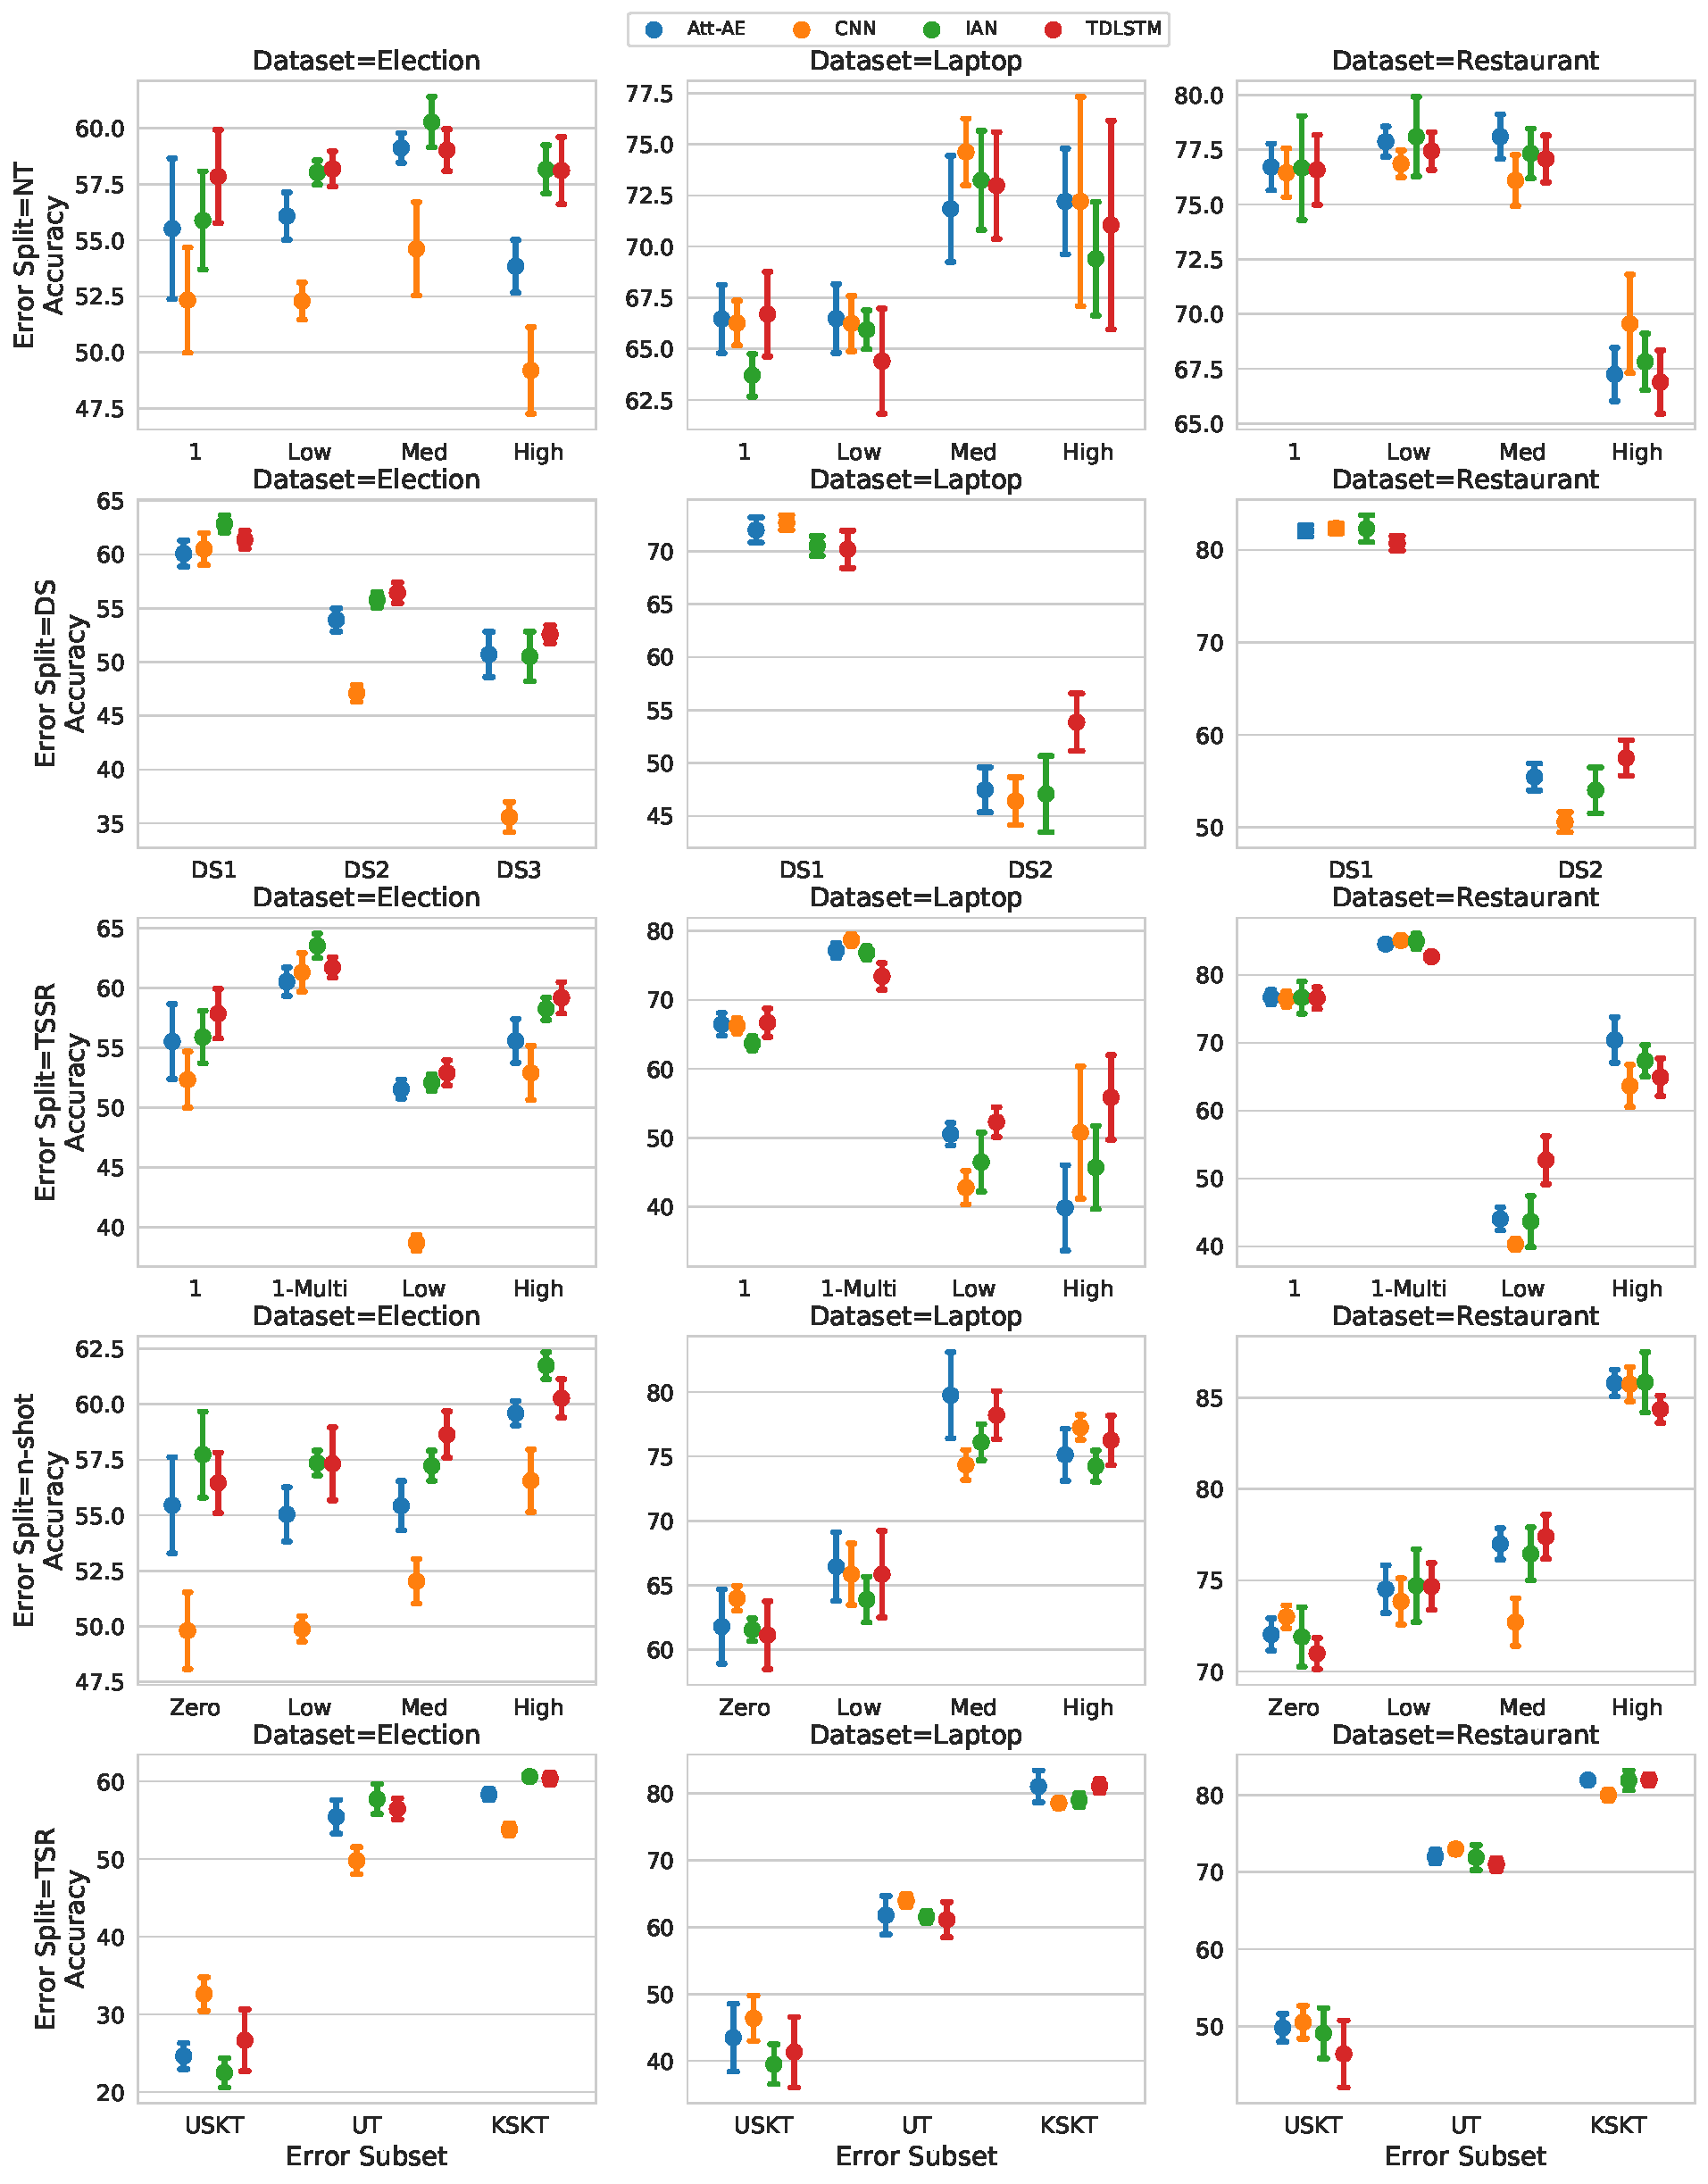
\includegraphics[scale=0.43]{images/augmentation/methods_performance/baseline/test_error_subsets.pdf}
    \caption{The mean and standard deviation error bars for each error subset within all of the error splits on the test split across all datasets.}
    \label{fig:aug_baseline_test_error_subset}
\end{figure}

\begin{figure}[h!]
    \centering
    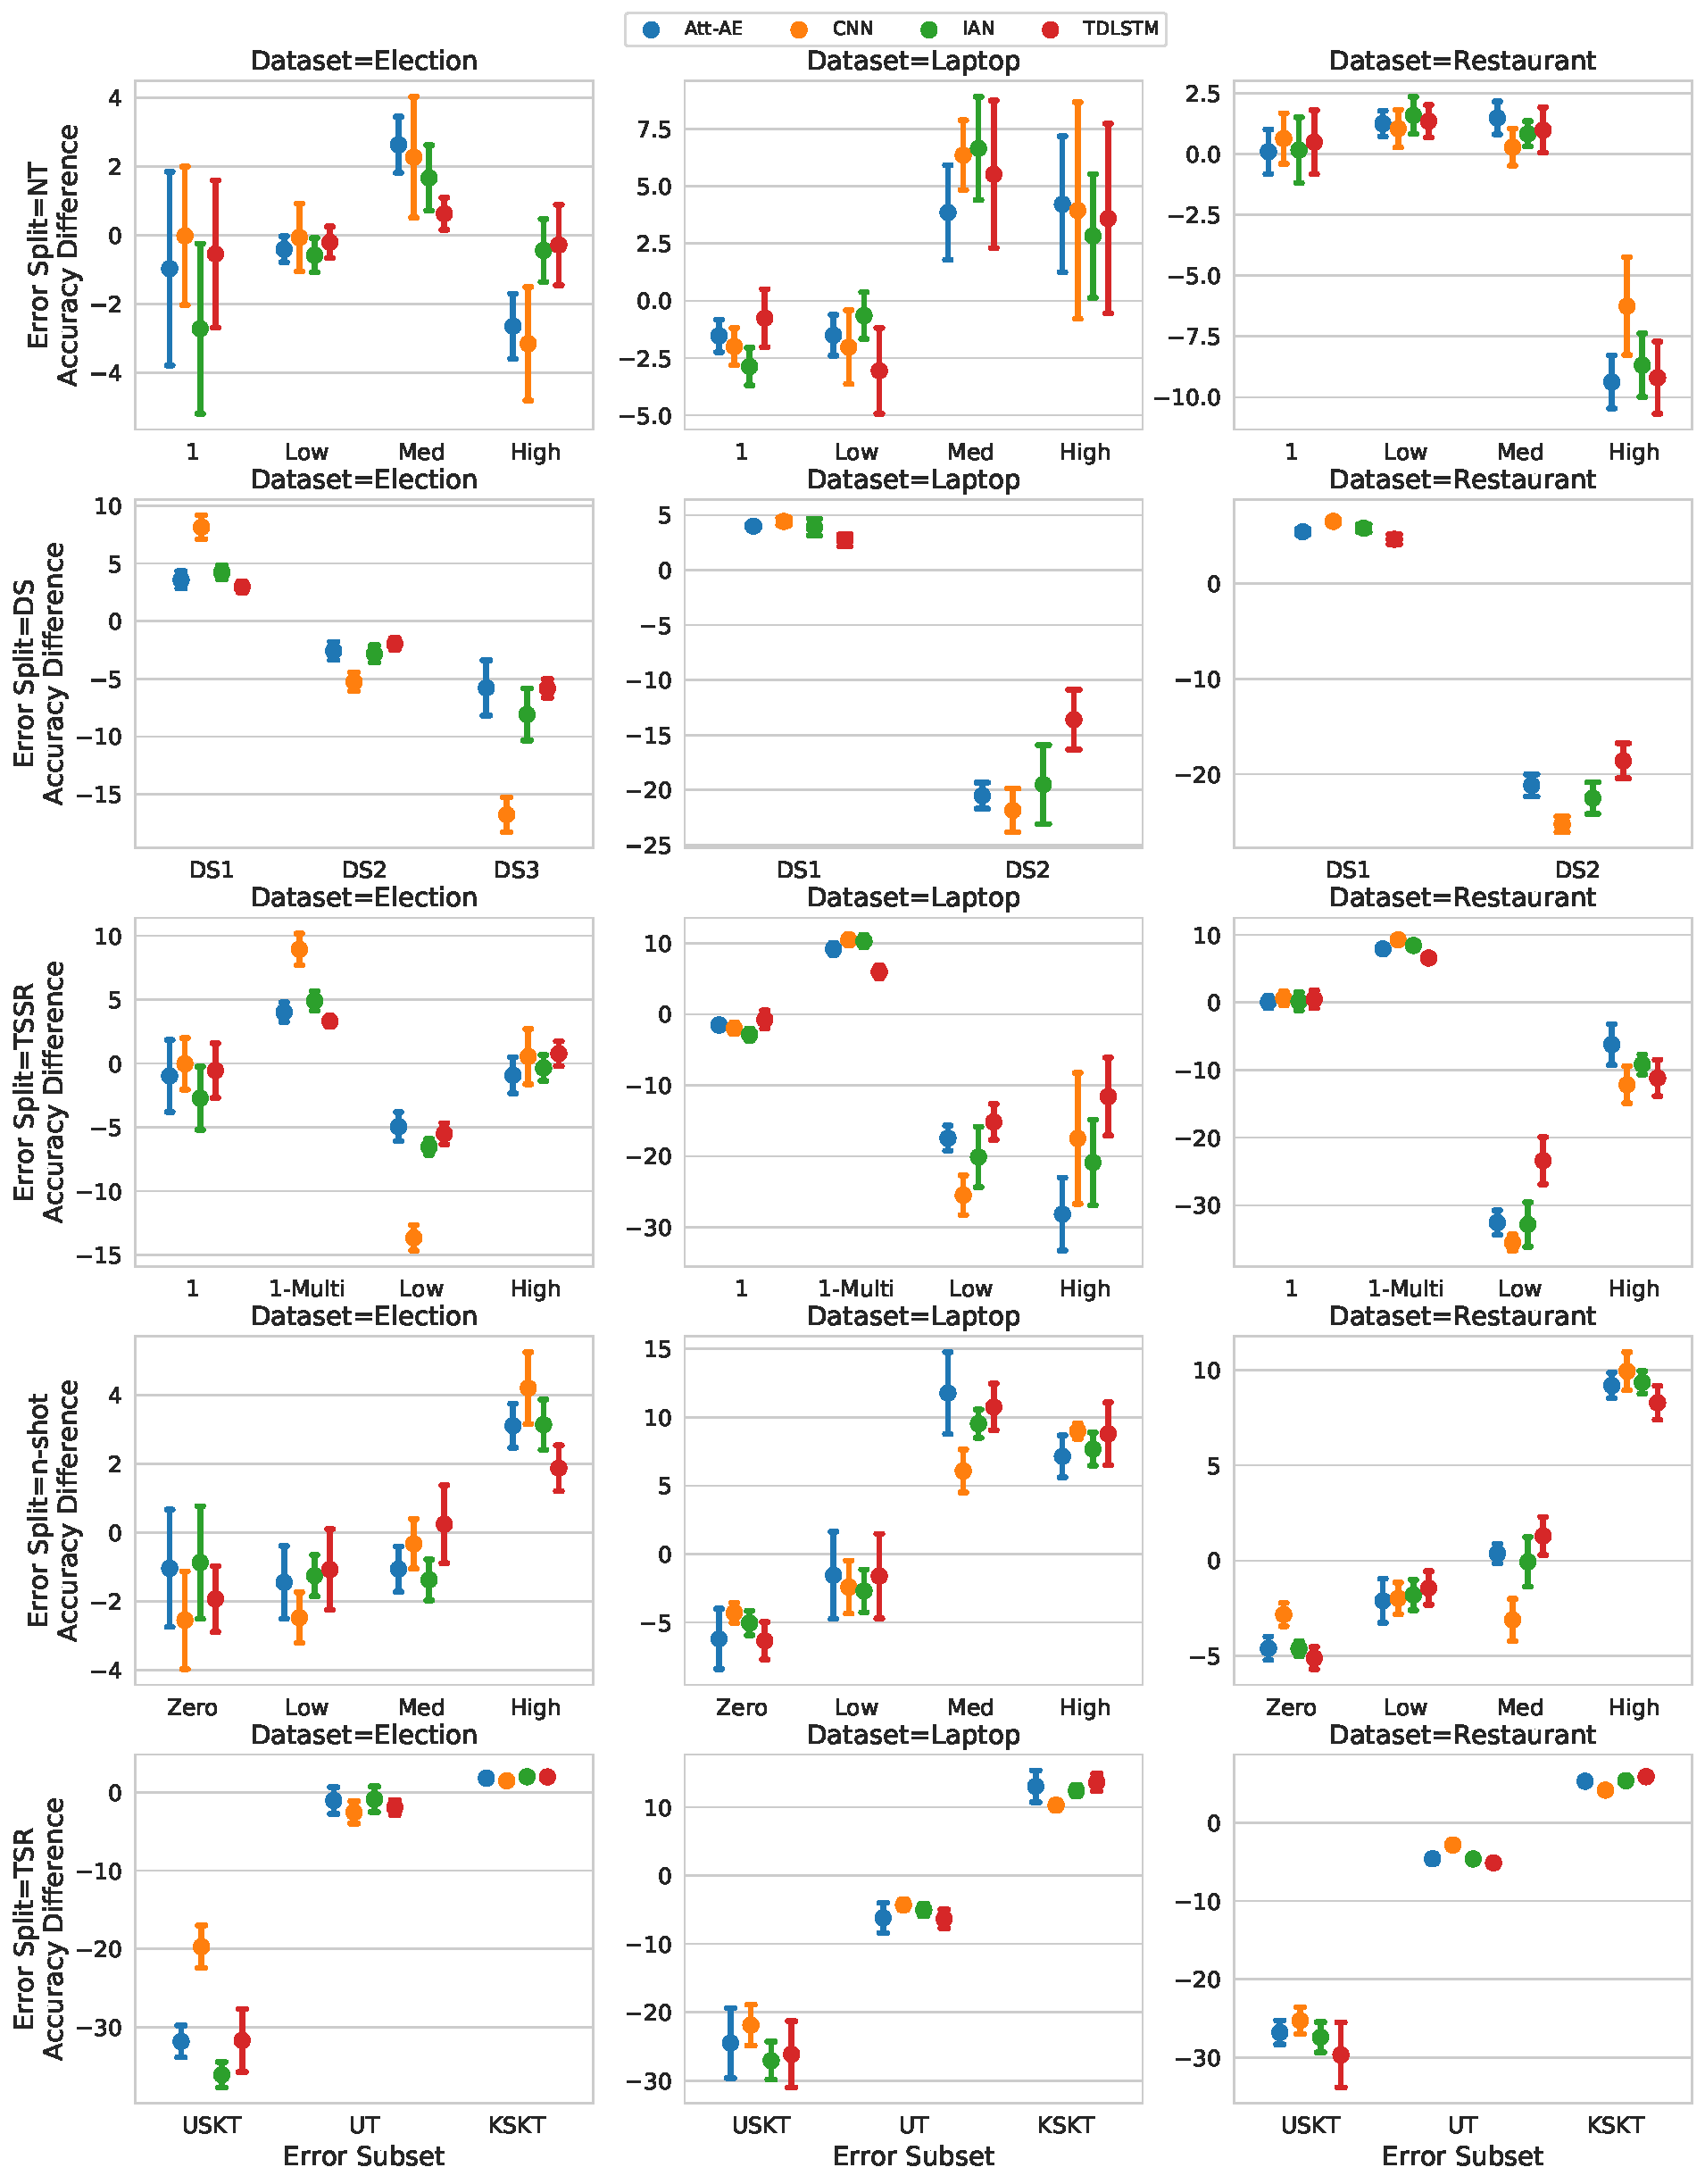
\includegraphics[scale=0.43]{images/augmentation/methods_performance/baseline/test_error_diff_subsets.pdf}
    \caption{The mean and standard deviation error bars for the difference between the overall accuracy and the accuracy from each error subset within all of the error splits on the test split across all datasets.}
    \label{fig:aug_baseline_test_error_diff_subset}
\end{figure}

\FloatBarrier
\subsubsection{Error Split Results Comparison between TDSA and Text Classification Models}

Using the test and validation results from the subsets shown in figures \ref{fig:aug_baseline_test_error_subset} and \ref{fig:aug_baseline_validation_error_subset} respectively it is possible to explore the differences between the text classification model and the TDSA models. These differences can be better seen through the heatmaps in figures \ref{fig:aug_baseline_dataset_error_subset_heatmap} and \ref{fig:aug_baseline_combined_dataset_error_subset_heatmap}, where the former is not corrected for multiple significance tests where as the later is using Bonferroni and is aggregated across datasets. Note that for figure \ref{fig:aug_baseline_dataset_error_subset_heatmap} the $DS_3$ subset results should be ignored for the Laptop and Restaurant datasets as they were never calculated as the sample size for the $DS_3$ subset is too small. Also the $DS_3$ subset is removed from figure \ref{fig:aug_baseline_combined_dataset_error_subset_heatmap} as only the Election dataset contains enough samples to create confidence scores. From all of these figures it is clear to see that the subsets that the TDSA models outperform the text classification model in are $DS_2$, $DS_3$, \textit{low-TSSR}, \textit{TSR KSKT}, \textit{n-shot Med}, and \textit{NT Low}. There are other subsets where the difference is significant as shown in the heatmaps but the majority of these significant differences only occur because of the Election dataset as can be seen if you compare figures \ref{fig:aug_baseline_dataset_error_subset_heatmap} and \ref{fig:aug_baseline_combined_dataset_error_subset_heatmap}. Furthermore, the outliers in these differences are the \textit{n-shot Med}, and \textit{NT Low} subsets of which the reason why it is believed these are outliers was described in the previous paragraphs. The $DS_2$, $DS_3$, and the \textit{low-TSSR} are expected to perform better for the TDSA models as they contain multiple unique sentiments within a sentence, for which a text classification model can only predict one of those sentiments for the sentence thus, limiting the model's capability to perform well on these subsets. This therefore shows that the TDSA models must be learning some target sentiment relationship modelling or else they would not be more competitive than the text classifier. The \textit{TSR KSKT} shows that when the TDSA models have seen a target enough times in a known sentiment context then they can perform a lot better than the text classification model and their respective overall accuracy. However it is the other subsets within \textit{TSR} that are of more interest showing the deficiencies of the TDSA models. The worse subset within \textit{TSR} is the \textit{USKT} of which this is the only subset where the text classification model in general perform significantly better (see figure \ref{fig:aug_baseline_combined_dataset_error_subset_heatmap}). TDSA models are most likely biasing the target representation towards a subset of sentiment classes for those targets and hence why the text classification models perform better on those targets. The \textit{UT} (\textit{n-shot zero} is the same subset) subset is an interesting result as it is dataset dependent as shown best in \ref{fig:aug_baseline_dataset_error_subset_heatmap}, in the Election dataset the TDSA models are better but in all other datasets the text classification model is better. This could be due to the size of the datasets as the Election dataset is much larger than the rest and therefore could allow the TDSA models to create better general target representations, thus allowing the models to leverage similarities with known targets. From the dataset heatmap figure \ref{fig:aug_baseline_dataset_error_subset_heatmap} it can be easily seen that on the Election dataset the majority of subsets are statistically significant compared to the Laptop and Restaurant dataset. This is most likely due to the Election dataset containing more targets per text (as can be seen in table \ref{table:augmentation_combined_dataset_statistics} \footnote{Dataset statistics for the splits, rather than the whole dataset, used in this section can be seen in table \ref{table:augmentation_splits_dataset_statistics}.}) and therefore far fewer texts within $DS_1$ which is the subset the text classification model is most suited to. Even though the text classifier does not perform  statistically significantly better than all the TDSA models on the Laptop and Restaurant datasets for $DS_1$ they are never worse. Furthermore, as the Laptop and Restaurant datasets are mainly made up of $DS_1$ samples (see figure \ref{fig:aug_error_analysis_ds}) this is most likely the reason why the TDSA models are not statistically significantly better than the text classification models on these datasets.



\begin{figure}[ht!]
    \centering
    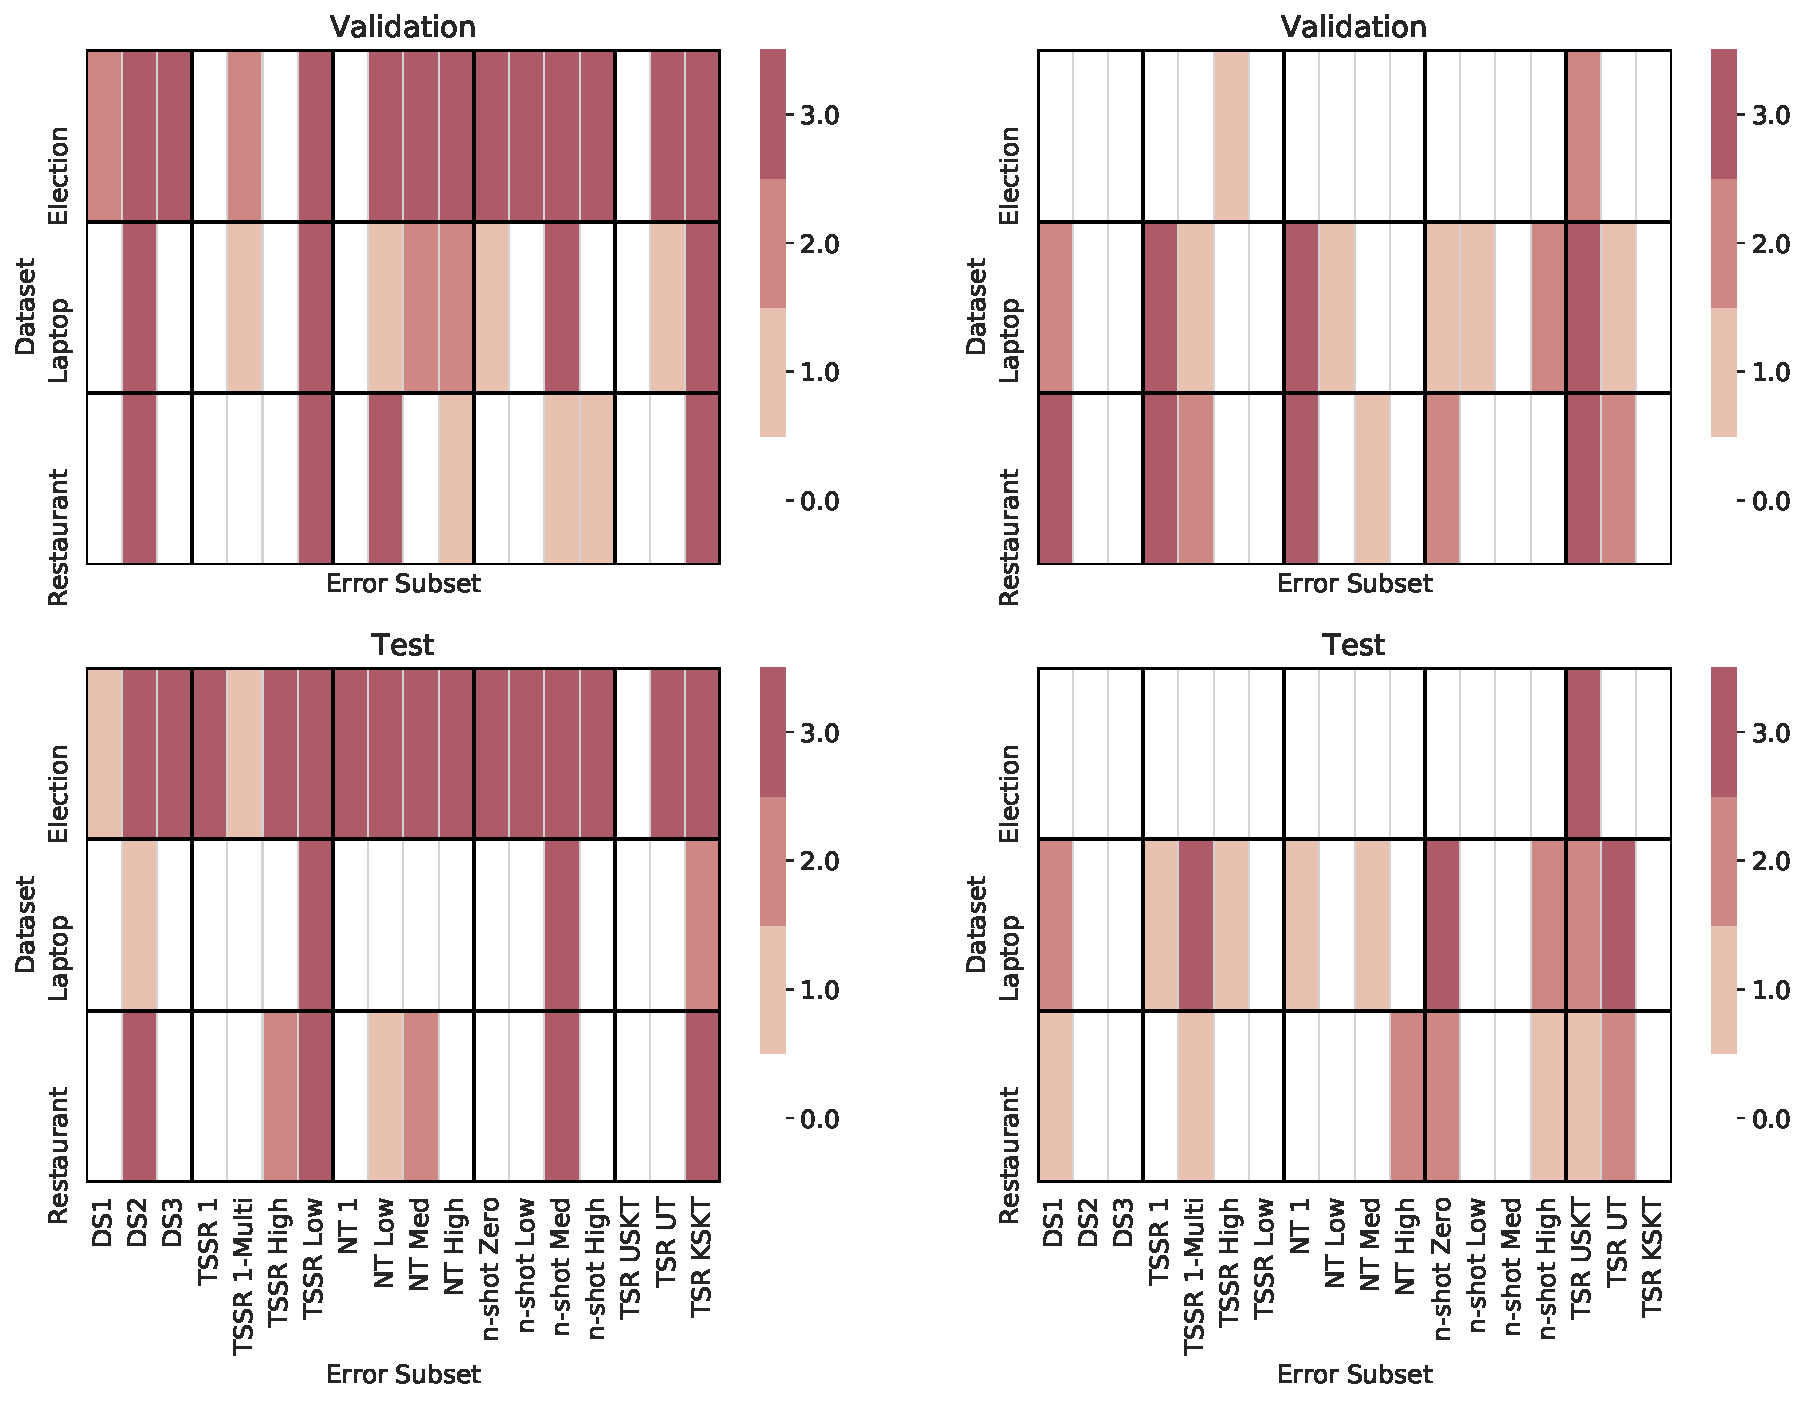
\includegraphics[scale=0.45]{images/augmentation/methods_performance/baseline/baseline_dataset_error_subset_heatmap.pdf}
    \caption{Plots in the first column represent the number of TDSA models that are statistically significantly better than the text classification model. Plots in the second column show the opposite, the number of TDSA models where the text classification is statistically significantly better. All plots have a confidence level of 95\% ($p \leq 0.05$).}
    \label{fig:aug_baseline_dataset_error_subset_heatmap}
\end{figure}

\begin{figure}[ht!]
    \centering
    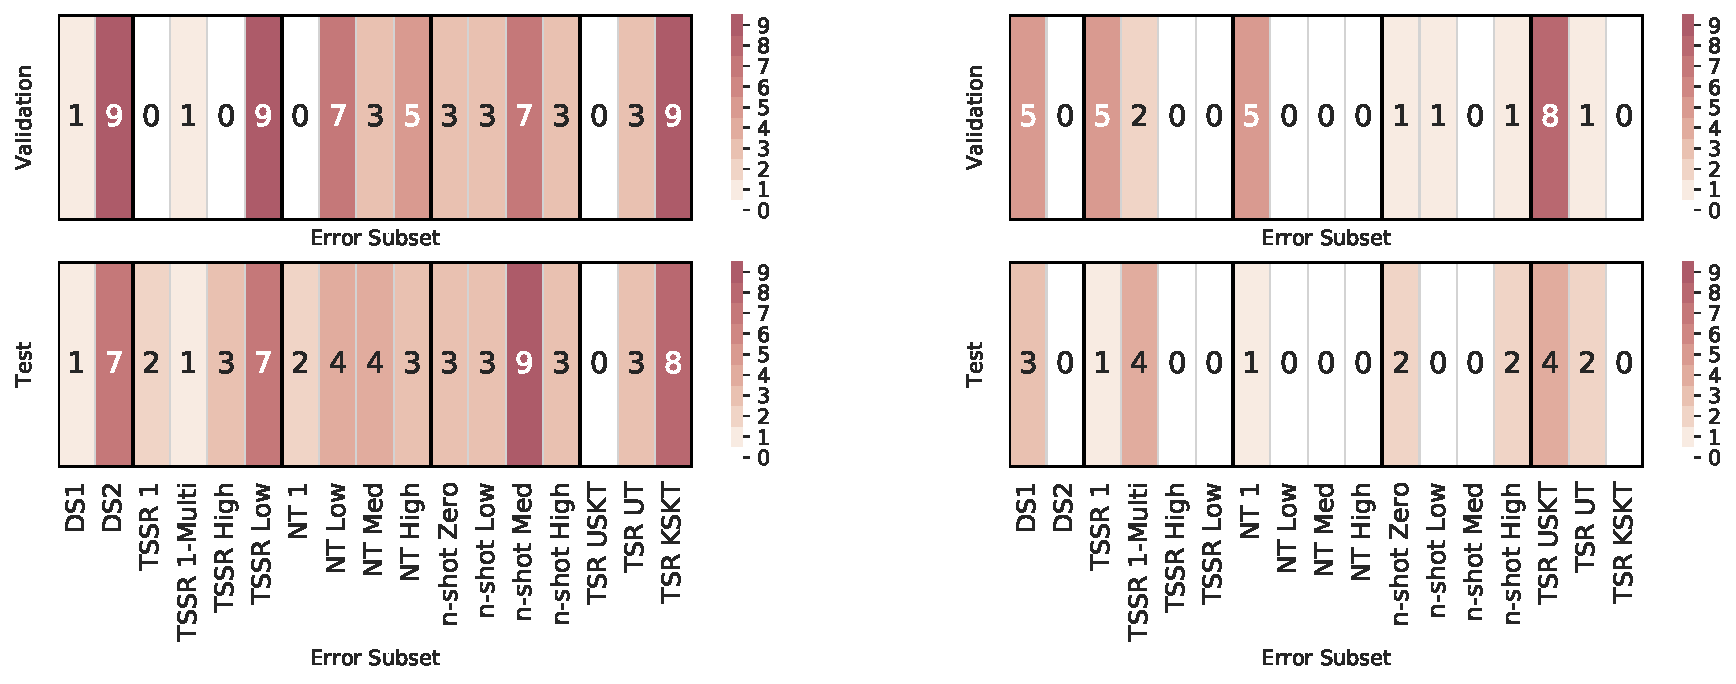
\includegraphics[scale=0.48]{images/augmentation/methods_performance/baseline/baseline_combined_dataset_error_subset_heatmap.pdf}
    \caption{Plots in the first column represent the number of TDSA models that are statistically significantly better than the text classification model across all datasets. Plots in the second column show the opposite, the number of TDSA models where the text classification is statistically significantly better. All plots have a confidence level of 95\% ($p \leq 0.05$) and have been corrected using Bonferroni.}
    \label{fig:aug_baseline_combined_dataset_error_subset_heatmap}
\end{figure}


\afterpage{
    \begin{landscape}% Landscape page
            \centering
            \begin{longtable}{|c|c|c|c|c|c|c|c|}
\hline
Name &  No. Sents(t) &  No. Targs (Uniq) &  ATS(t) & POS (\%) & NEU (\%) & NEG (\%) \\
\hline
Laptop &              1872 &         2950 (1181) &    1.58 &  1328 (45.02) &   628 (21.29) &   994 (33.69) \\
\hline
Restaurant &              2578 &         4722 (1528) &    1.83 &  2892 (61.25) &   829 (17.56) &   1001 (21.2) \\
\hline
Election &              4045 &        11899 (2179) &    2.94 &  1744 (14.66) &  4572 (38.42) &  5583 (46.92) \\
\hline
\multicolumn{7}{|p{0.9\linewidth}|}{No. Sents(t)=number of sentences that contain a target, No. Targs (Uniq)=Number of (unique) targets (all targets are lower cased), ATS(t)=Average Target per Sentence where the sentences must contain a target, LABEL (\%)=Number of LABEL samples (percentage of LABEL samples).} \\
\hline
\caption{Dataset statistics for each datasets where each dataset represent the combination of all the dataset's splits e.g. train, validation, and test.}
\label{table:augmentation_combined_dataset_statistics}
\end{longtable}
    \end{landscape}
}

\newpage
\FloatBarrier
\subsubsection{Comparing the Error Split Results to the Prior Work}
\label{section:augmentation_cwr_comparing_to_prior_work_new}
% How does all of this relate back to the previous work this needs to be moved up to above the NT stuff.
From the results in this subsection the findings can relate back to some of the original work on these splits confirming the same findings. The findings of the \textit{TSSR 1-Multi} performing better than \textit{TSSR 1} is the same finding as \citet{nguyen-shirai-2015-phrasernn} as both of these subsets are the equivalent to \textit{ST2} and \textit{ST1}. When the number of unique sentiments increase in a text, which can be measured through the \textit{DS} and \textit{TSSR} splits, this reduces the performance of a method, which is the same finding as \citet{xue-li-2018-aspect} comparing the normal test to the \textit{hard} test, and that of \citet{nguyen-shirai-2015-phrasernn} comparing \textit{ST1} or \textit{ST2} with \textit{ST3}.  

The \textit{n-shot} findings do not confirm the findings of the original work by \citet{yang2018multi} where they found that in general models performance do not correlate with the number of times the target/aspect appeared in the training data. However, our findings show that they do correlate where the more the target appears in the training data the better the performance in general. The reason for the difference could come from the task itself, as \citet{yang2018multi} was not solving the task of TDSA but rather the task of Multi-Entity Aspect Based Sentiment Analysis (ME-ABSA), where TDSA would be equivalent if when predicting the sentiment of the target the latent aspect was also given. This difference in task could make a large difference as knowing a target's latent aspect could greatly improve a model's performance on unknown targets. The reason why the latent aspect would make such a large difference is because the dataset would contain a few aspects which occur frequently therefore allowing the model to create a good representation for the aspects. Furthermore, given these aspects the likelihood is that there could be many unknown aspect target pairs but due to the model potentially having a good representation of the aspect the performance on these \textit{zero-shot} pairs could be quite high. Thus, a reason for \citet{yang2018multi} finding no correlation between performance and number of times the target/aspect appeared in the training data could be due to the aspects.

%
% The above three paramgraphs need to be merged with the one below. as need to add a paragraph on DS
%
% The \textit{NT} split by \citet{zhang-etal-2019-aspect} which was found to be unstable in that original work and similar in this thesis, was to some extent explained empirically why it was for the first time in this thesis. The reason in \citet{zhang-etal-2019-aspect} work to overcome the stability was to better model inter target dependencies (target interaction). However considering the empirical evidence put forward here as shown in figures \ref{fig:aug_baseline_ds_nt_test_scores} and \ref{fig:aug_baseline_tssr_nt_test_scores}, the belief is that the \textit{NT} split itself does not measure target interaction and a dataset that does so would be a more suitable suggestion.

As found earlier in figures \ref{fig:aug_baseline_test_error_subset} and \ref{fig:aug_baseline_validation_error_subset} for the test and validation results respectively the \textit{NT} split does not show any consistent trend, which to some degree is what is found in the original works \citep{he-etal-2018-effective,zhang-etal-2019-aspect}. The expected trend was as the number of targets increase the lower the performance. A potential reason for this could be that there are other factors that influence the \textit{NT} split. The factors that will be explored here are the target sentiment relationship factors which can be measured to some extent using the \textit{DS} and \textit{TSSR} splits. To explore this all the datasets will be first subsetted by one of the \textit{DS} or \textit{TSSR} subsets and then further subsetted by one of the \textit{NT} subsets, the model's performance will be measured on each one of these compounded subsets. Figures \ref{fig:aug_baseline_ds_nt_test_scores} and \ref{fig:aug_baseline_tssr_nt_test_scores} show the performance on these compounded subsets whereby the former subsets the data by \textit{DS} and the latter \textit{TSSR}, for the validation data this can be seen in figures \ref{fig:aug_baseline_ds_nt_validation_scores} and \ref{fig:aug_baseline_tssr_nt_validation_scores}. Note that in the figures some of the \textit{NT} subsets do not exist on the x-axis, this is because after the subset compounding no data exists for those subsets. These figures show that in general for the $DS_1$ and \textit{TSSR 1-Multi} rows the larger \textit{NT} the better the performance of the models, of which for the $DS_1$ row this can be better seen in the validation data (figure \ref{fig:aug_baseline_ds_nt_validation_scores}) than the test. This is most likely the case because of the models exploiting the fact that there are more targets expressing the same sentiment. This exploitation of targets expressing the same sentiment can also be seen in the $DS_2$ rows (better seen in the validation data) where the more targets the better the score. Within the \textit{Low} and \textit{High TSSR} subsets the trend is less clear. The expectation within these subsets would be, when there are more targets (larger \textit{NT}) this will results in poorer performance for the \textit{Low TSSR} subset, but better results for the \textit{High TSSR} subset. This expectation is under the assumption that the more targets there are within the \textit{High TSSR} subset the greater the likelihood that the targets have the same sentiment and exploiting the most frequent sentiment would gain a higher performance score. The opposite is true when there are more targets within the \textit{Low TSSR} subset the greater the likelihood that the targets have a different sentiment and exploiting the most frequent sentiment would gain a lower performance. However, this expectation is not always true and can be inconsistent between splits, for example the \textit{High TSSR} Laptop results have different trends between test and validation splits. Furthermore, this assumption of more targets within the \textit{TSSR Low} and \textit{High} subsets does not necessarily mean more targets of the most frequent sentiment class due to the way \textit{TSSR} subsets are created (equation \ref{eq:aug_tssr}), hence a potential reason why there is no consistent correlations in those subsets. Thus, this analysis shows to some extent why the \textit{NT} split has no trend as the target sentiment relationship factors are more influential than the number of targets on the performance of the models. This therefore solves to some extent why \citet{zhang-etal-2019-aspect}\footnote{See figure 4 in the paper.} and \citet{he-etal-2018-effective}\footnote{See figure 3 in the paper.} also could not find a steady trend for the \textit{NT} split.
%The $DS_2$, $DS_3$, \textit{High TSSR}, and \textit{Low TSSR} rows are less clear most likely due to the $DS_2$ and $DS_3$ containing data that can be in both \textit{Low} and \textit{High} \textit{TSSR} subsets. Thus as stated earlier the model could be overfitting to one sentiment in each sentence and hence why there are trends in the \textit{Low (High) TSSR} subset that when there are more (less) targets (higher \textit{NT}) the worse the results. This analysis shows that there are trends in the \textit{NT} subsets when sentiment relation factors have been taken into account as shown by subsetting the data first by one of the \textit{TSSR} or \textit{DS} subsets. Thus this analysis shows to some extent why the \textit{NT} split has no trend as the target sentiment relationship factors are more influential than the number of targets on the performance of the models. This therefore solves to some extent why \citet{zhang-etal-2019-aspect}\footnote{See figure 4 in the paper.} also could not find a steady trend for the \textit{NT} split. 

%This analysis however brings up the question of how to measure target interaction explicitly as the \textit{NT} split clearly cannot do this. Thus a dataset that has target interaction annotated would be of use to the community to better understand these models. However careful consideration will have to be taken when creating such a dataset so that other factors are not being measured at the same time. One could design such a dataset so that the only way a target can be predicted is through target to target interaction, and not possible via target sentiment relationship or most frequent sentiment class within the sentence. Thus it can be concluded that the \textit{NT} split is not fit for any purpose therefore will not be used after this subsection.

\begin{figure}[h!]
    \centering
    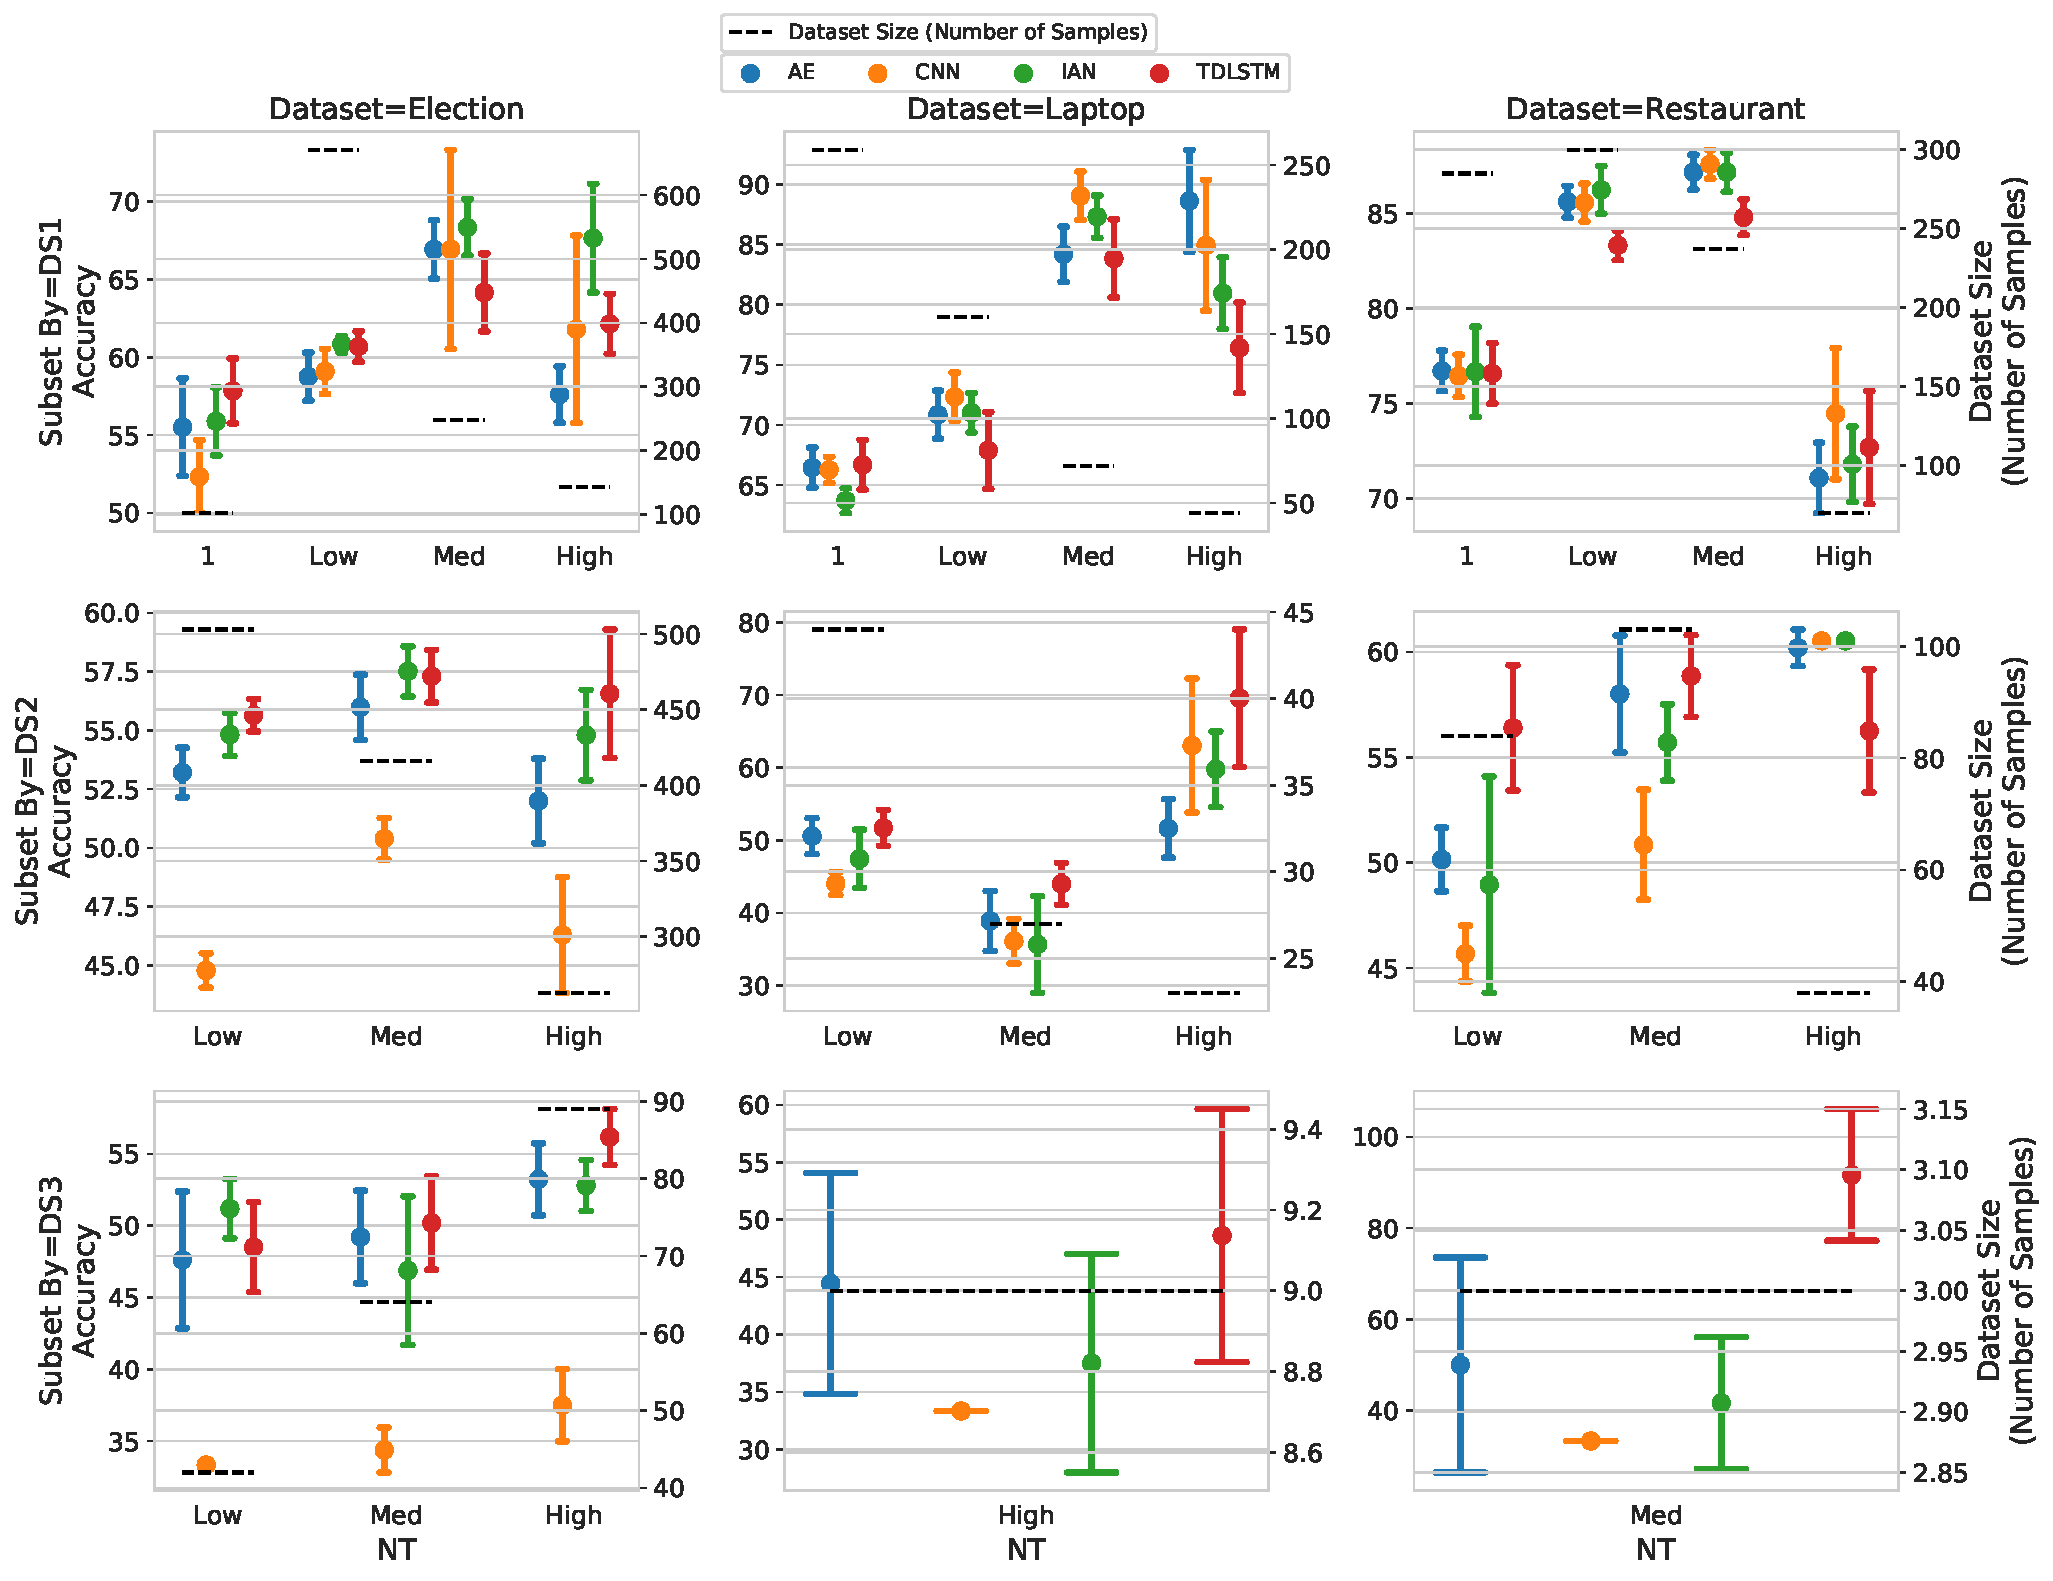
\includegraphics[scale=0.42]{images/augmentation/methods_performance/baseline/baseline_ds_nt_test_scores.pdf}
    \caption{Each plot shows the performance (y-axis accuracy) of the given models and sample size of the data evaluated on (y-axis dataset size) on the different test datasets (columns) after being subsetted by the relevant \textit{DS} subset (rows) and then NT subset (x-axis).}
    \label{fig:aug_baseline_ds_nt_test_scores}
\end{figure}
\begin{figure}[h!]
    \centering
    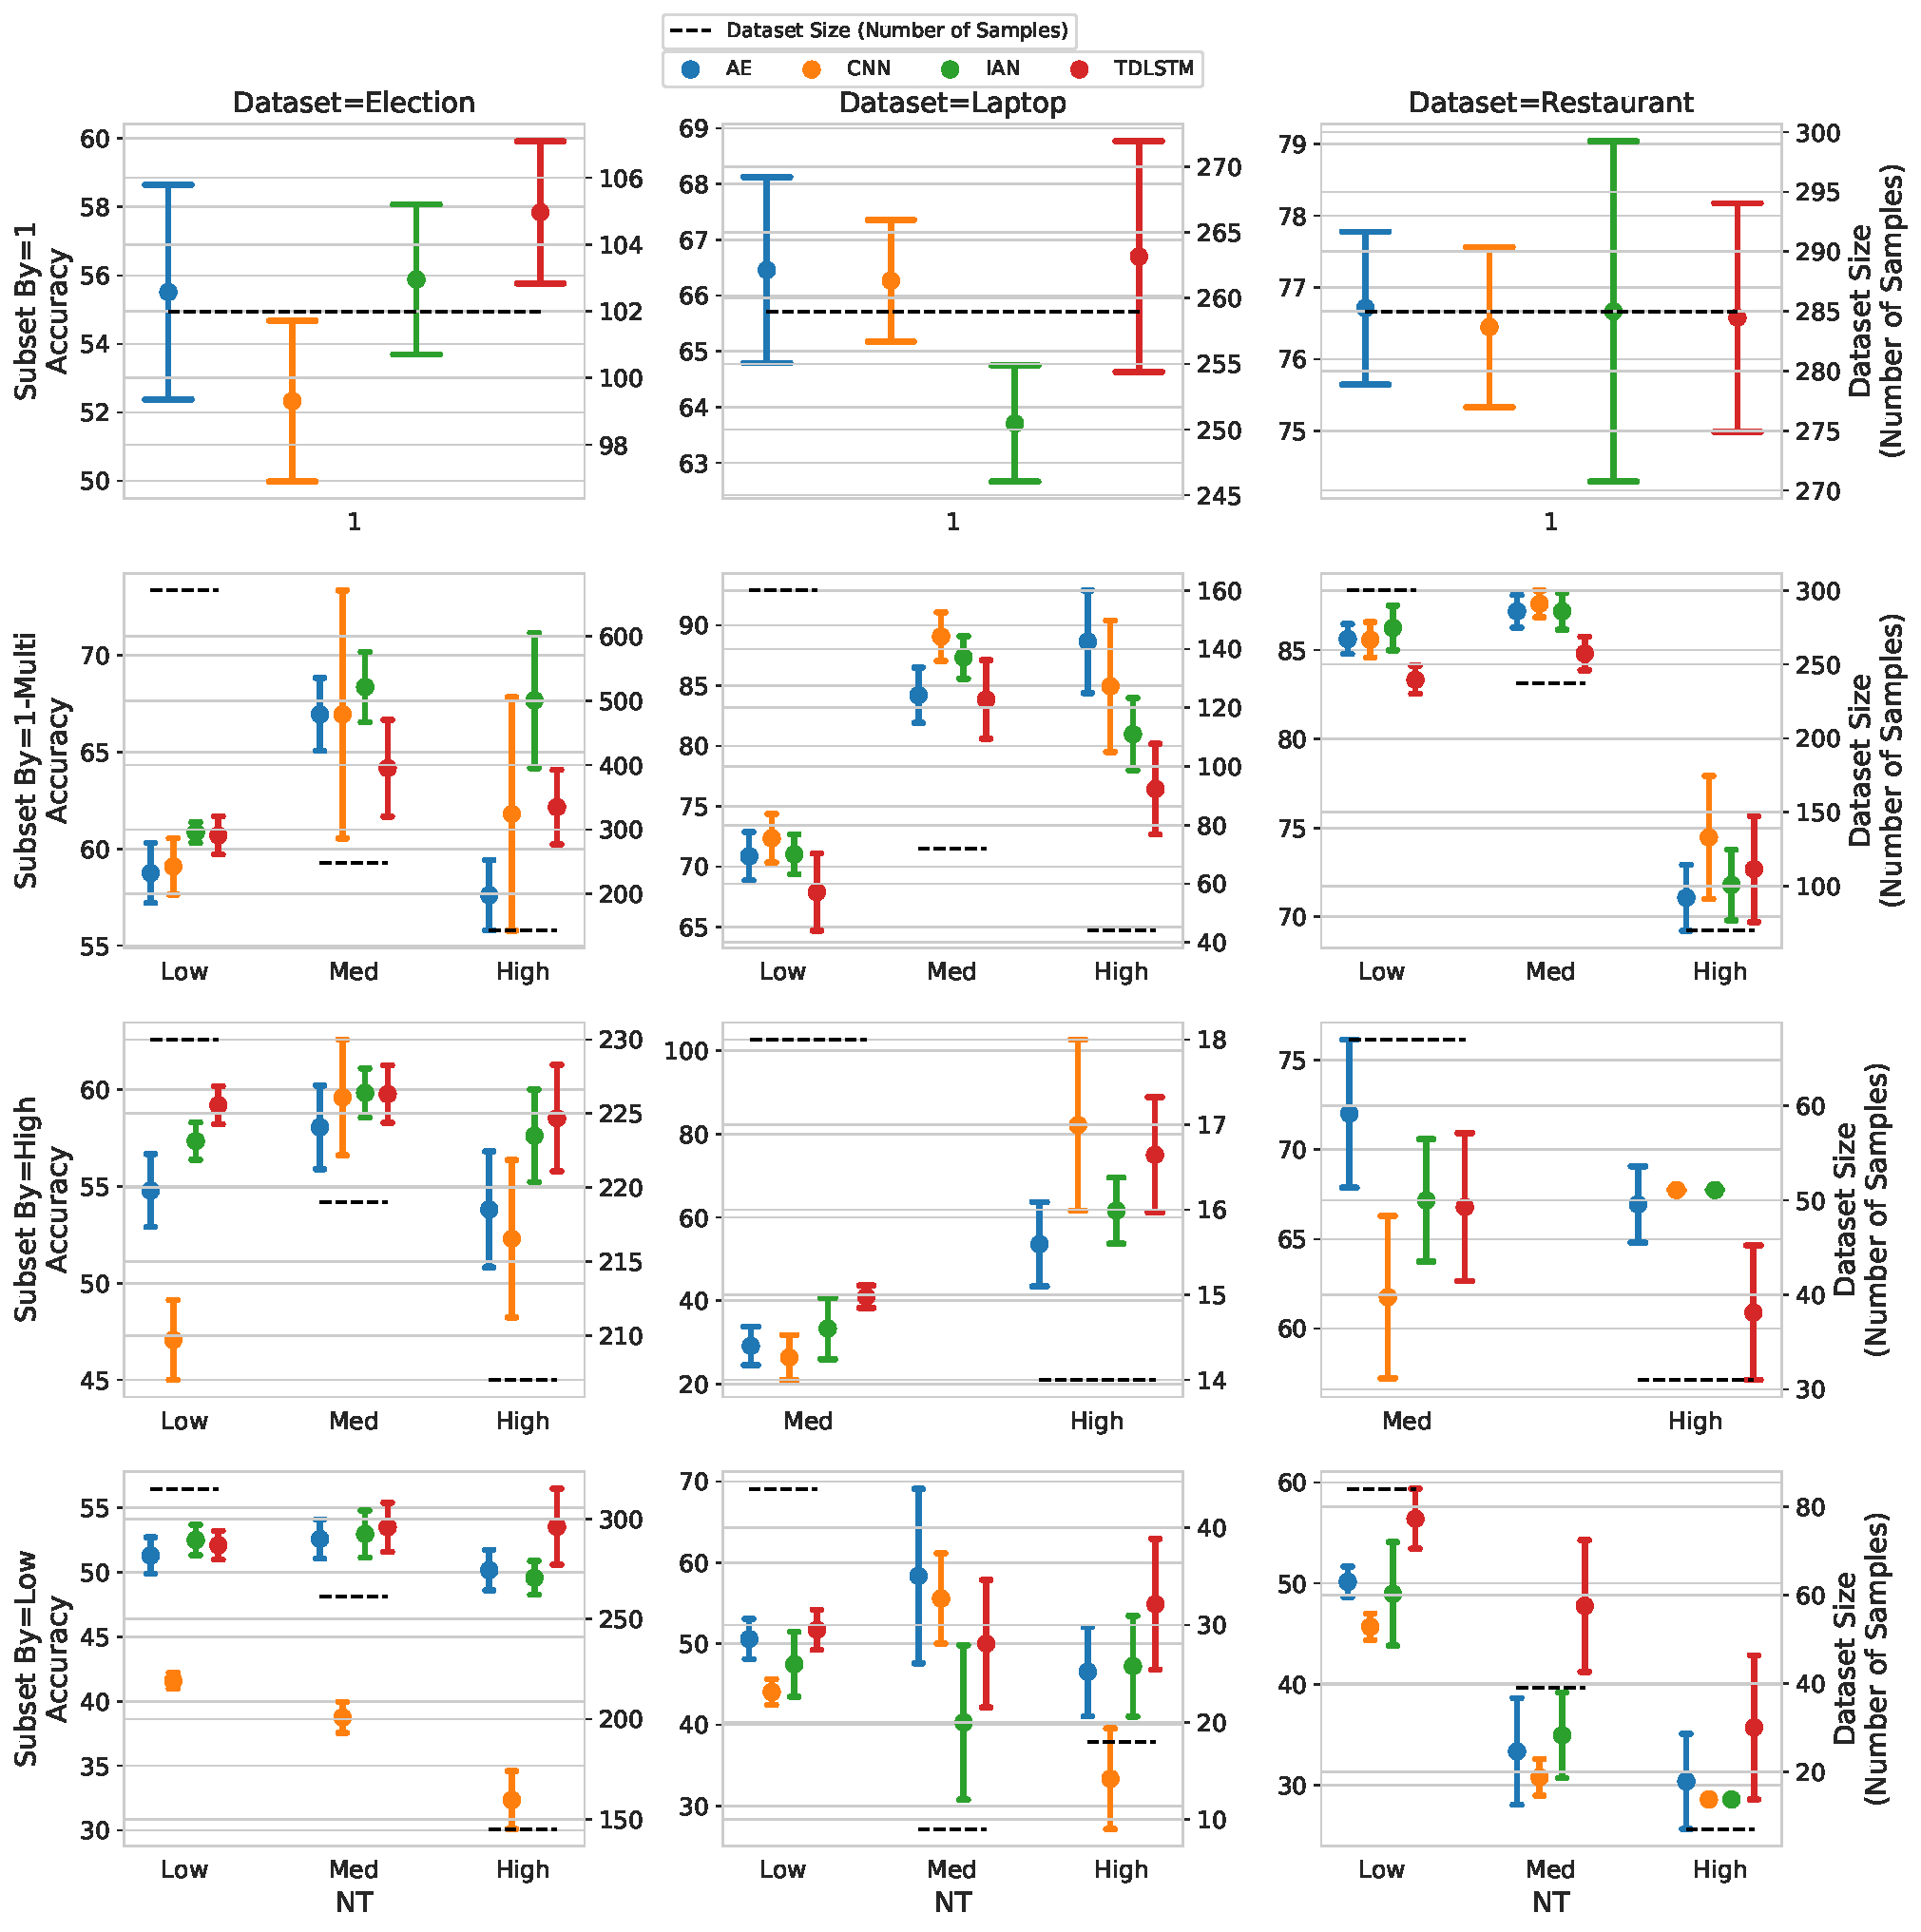
\includegraphics[scale=0.42]{images/augmentation/methods_performance/baseline/baseline_tssr_nt_test_scores.pdf}
    \caption{Each plot shows the performance (y-axis accuracy) of the given models and sample size of the data evaluated on (y-axis dataset size) on the different test datasets (columns) after being subsetted by the relevant \textit{TSSR} subset (rows) and then NT subset (x-axis).}
    \label{fig:aug_baseline_tssr_nt_test_scores}
\end{figure}

The $DS_i$ split was stated to get more difficult as $i$ increased and this has been shown in this work and in the original \citep{wang-etal-2017-tdparse}. However, as mentioned in section \ref{section:aug_error_analysis_previous_work}, in the original work it was also shown for some methods and metrics that the models perform best on the $DS_3$ subset. In this work that phenomena did not occur when using the accuracy metric, which \citet{wang-etal-2017-tdparse} did not use. Therefore, to test if the \textit{DS} split results do change because of the metric, in figure \ref{fig:aug_baseline_sentiment_f1_ds_all} are the \textit{DS} results on all datasets using the macro F1 metric which was one of the metrics used by \citet{wang-etal-2017-tdparse}. As can be seen from the results the only dataset where $i$ in $DS_i$ does not negatively correlate with the macro F1 results is the Election test dataset. The Election test datasets was also the only dataset \citet{wang-etal-2017-tdparse} used when measuring model performance on the \textit{DS} split\footnote{Results can be found in table 4 of \citet{wang-etal-2017-tdparse}.}. The other results follow the trend shown in this section when using the accuracy metric. 

\begin{figure}[h!]
    \centering
    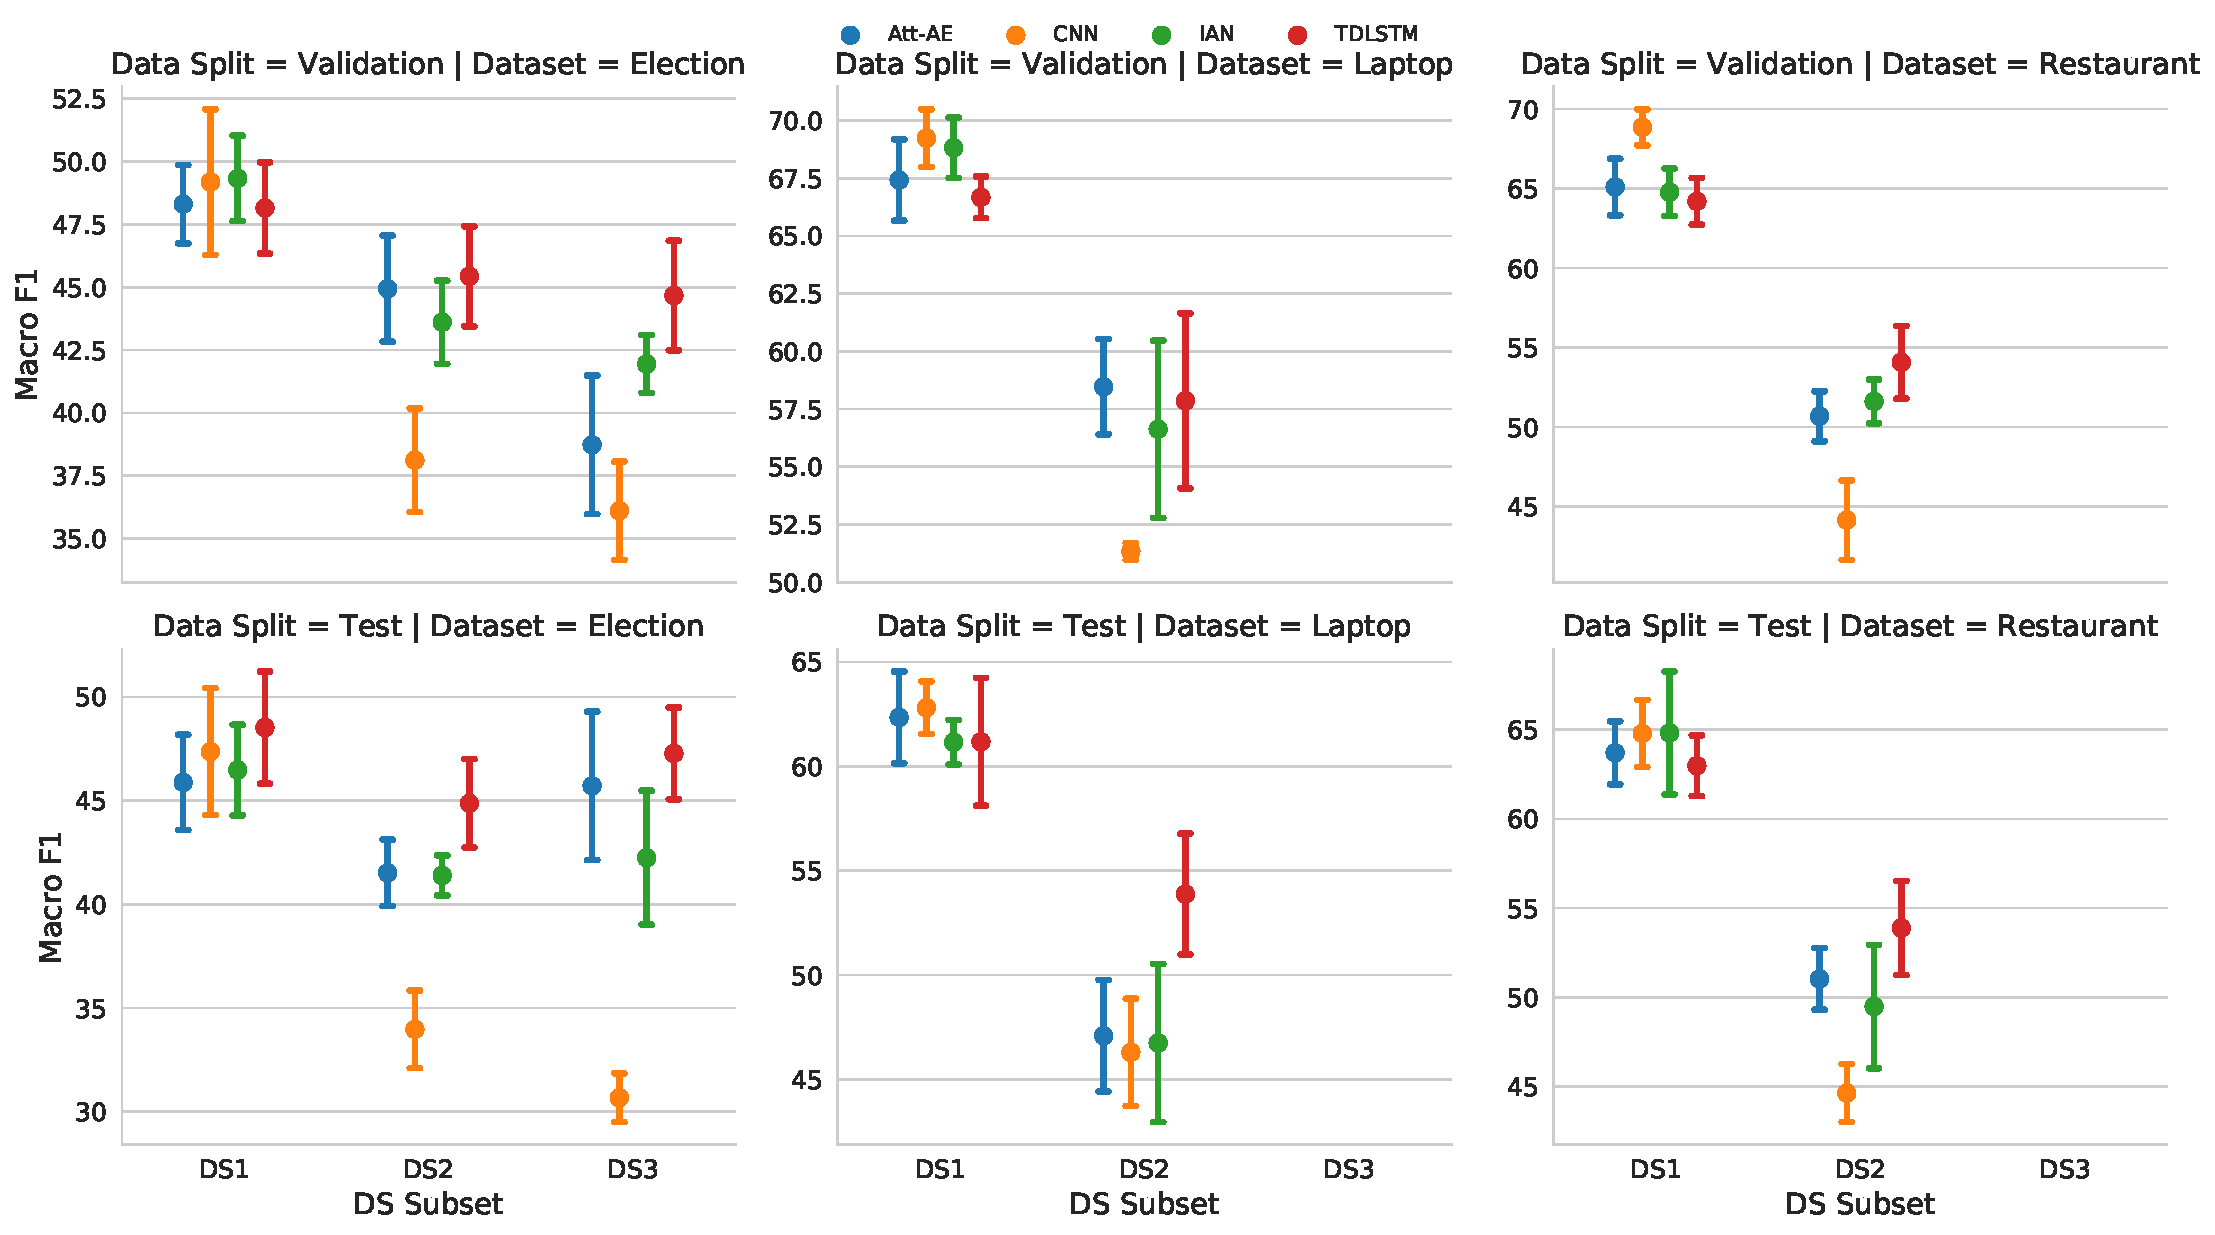
\includegraphics[scale=0.38]{images/augmentation/methods_performance/baseline/sentiment_f1_ds_all.pdf}
    \caption{Macro F1 score where the data is subsetted by the \textit{DS} split.}
    \label{fig:aug_baseline_sentiment_f1_ds_all}
\end{figure}

To investigate why the Election test dataset does have a different trend when using a different metric the approach taken was to explore the individual F1 scores for each sentiment label on the Election dataset. This approach was taken as the main difference between accuracy and macro F1, as the macro F1 is not biased by the un-balanced label distribution that is within the dataset, of which all datasets used are very un-balanced (see table \ref{table:augmentation_combined_dataset_statistics}). Figure \ref{fig:aug_baseline_sentiment_f1_ds_election} shows the results of each sentiment label's F1 score and as expected the most frequent sentiment (negative) has the highest scores no matter the subset. These results highlight why the macro F1 score does not have the same negative correlation as the accuracy metric does for the \textit{DS} split. As the results show the positive and the neutral sentiments do not follow the negative correlation that the negative sentiment does. Thus, as the scores of each sentiment are weighted the same in the macro F1 metric this therefore causes the macro F1 score for the $DS_3$ subset to be higher than the $DS_2$ subset in the test split. The potential reason for this unusual correlation could be due to the model overfitting to the most frequent sentiment class (negative) and hence why if the model predicted negative for all samples in a $DS_3$ sentence then it would get some samples correct but it would get at least 2 samples wrong.

\begin{figure}[h!]
    \centering
    \includegraphics[scale=0.38]{images/augmentation/methods_performance/baseline/sentiment_f1_ds_election.pdf}
    \caption{The Election test and validation split F1 scores for each sentiment label, where the data has been further broken down through \textit{DS} subsets.}
    \label{fig:aug_baseline_sentiment_f1_ds_election}
\end{figure}

To further investigate whether the most frequent sentiment class always has this negative correlation the results for the Restaurant and Laptop datasets are shown in figures \ref{fig:aug_baseline_sentiment_f1_ds_restaurant} and \ref{fig:aug_baseline_sentiment_f1_ds_laptop} respectively. From these two plots we can see that the most frequent sentiment class (positive for both datasets) has the largest drop in F1 score from $DS_1$ to $DS_2$. This large drop in F1 score gives some extra merit to the idea that the models are overfitting to the most frequent sentiment class\footnote{It was also found in chapter \ref{chapter:reproducibility} section \ref{section:repro_mass_eval} that NN based methods overfit to the most frequent sentiment class on many datasets in a low resource setting.}. Due to this overfitting the model is most likely predicting the most frequent sentiment class more often than it should where as in the cases for the least frequent sentiment classes it could be only predicting these when it is confident. These reasons are not empirically proven but the results have shown further insight into the \textit{DS} split. Lastly, these results show more that the results from the original paper \citep{wang-etal-2017-tdparse} do not generalise across datasets and that the general result is that the metrics normally correlate negatively with the \textit{DS} subsets. 

\begin{figure}[h!]
    \centering
    \includegraphics[scale=0.38]{images/augmentation/methods_performance/baseline/sentiment_f1_ds_restaurant.pdf}
    \caption{The Restaurant test and validation split F1 scores for each sentiment label, where the data has been further broken down through \textit{DS} subsets.}
    \label{fig:aug_baseline_sentiment_f1_ds_restaurant}
\end{figure}
\begin{figure}[h!]
    \centering
    \includegraphics[scale=0.38]{images/augmentation/methods_performance/baseline/sentiment_f1_ds_laptop.pdf}
    \caption{The Laptop test and validation split F1 scores for each sentiment label, where the data has been further broken down through \textit{DS} subsets.}
    \label{fig:aug_baseline_sentiment_f1_ds_laptop}
\end{figure}

\FloatBarrier
\subsection{The Strict Text ACcuracy (STAC) Metric}
\label{section:augmentation_cwr_STAC_new}

Both the \textit{DS} and \textit{TSSR} error splits explore the concepts of target sentiment relationships and overfitting to the most common sentiment within a text. However, neither of these can create error subsets that will explicitly inform you if the model can detect sentiment for all the targets in the text and thus performing the target sentiment relationship task perfectly. Both the \textit{DS} and \textit{TSSR} splits do attempt to show this but both are subject to the model finding the most frequent or easiest to find sentiment for some/all of the targets in the subsets. Thus, the creation of the Strict Text ACcuracy (\textit{STAC}) metric. This metric works on the sentence/text level compared to the accuracy and macro F1 metrics that are based at the target level. \textit{STAC} treats each sentence as a sample and each sentence can only be correct if all targets within that sentence have been classified correctly, it is then averaged by the number of sentences. The \textit{TAC} equation \ref{eq:aug_tac} that is used within the \textit{STAC} equation \ref{eq:aug_stac} finds the average number of targets that are correct within a sentence. The notation to describe \textit{STAC} and \textit{TAC} in equations \ref{eq:aug_stac} and \ref{eq:aug_tac} is the same notation used in equation \ref{eq:aug_tssr}, which describes the \textit{TSSR} split. $T_j$ within \textit{STAC} represents all of the targets within sentence $j$ from all sentences $X$ that is within the dataset, and $t_{ji}$ represents target $i$ true sentiment within sentence $T_j$ where $\hat{t_{ji}}$ is the predicted sentiment.

\begin{equation}
    \text{Text ACcuracy (TAC)}(T_j) = \frac{\sum_{i=1}^{|T_j|} [t_{ji}=\hat{t_{ji}}]}{|T_j|}
    \label{eq:aug_tac}
\end{equation}
\begin{equation}
    \text{Strict Text ACcuracy (STAC)} = \frac{\sum_{j=1}^{|X|} \begin{cases}
    1,& \text{if } \text{TAC}(T_j) = 1\\
    0,              & \text{otherwise}
\end{cases}}{|X|}
\label{eq:aug_stac}
\end{equation}

The \textit{STAC} metric is more useful when applied to subsets of a dataset, thus two specific versions of the \textit{STAC} metric are created:
\begin{enumerate}
    \item \textit{STAC 1} - The \textit{STAC} metric applied to only the data in the $DS_1$ subset.
    \item \textit{STAC Multi} - The \textit{STAC} metric applied to only the data in the $DS_2$ and $DS_3$ subsets.
\end{enumerate}

The \textit{STAC Multi} gives in one metric how well overall a TDSA model is at target sentiment relation modelling removing all factors of overfitting to a sentiment class, or predicting the most frequent sentiment, of which this is possible in \textit{STAC 1}. \textit{STAC Multi} can also be seen as a coarse grained and much stricter version of the \textit{DS} split, as both measure target sentiment relationship modelling. However, due to \textit{STAC Multi} being such a strict and thus difficult metric the \textit{DS} subsets can be useful to measure target sentiment relationship modelling at a more fine grained scale. For example, if a model does not perform significantly better nor worse than another on \textit{STAC Multi} but does perform better on $DS_2$ and $DS_3$ subsets, then the likelihood is that the model is performing target sentiment relationship modelling better. The difference between \textit{STAC 1} and \textit{STAC Multi} can show to some degree how much the model is overfitting to the most frequent sentiment class in a text. The performance of all models across all metrics including accuracy and macro F1 can be seen in \ref{fig:baseline_stac_scores.png}, the \textit{STAC} metric is shown for completeness. As can be seen from the figure the \textit{STAC Multi} is by far the most difficult metric and scores much lower than any of the accuracy metrics on any of the subsets shown in figure \ref{fig:aug_baseline_test_error_subset} (validation split figure \ref{fig:aug_baseline_validation_error_subset}). However, the \textit{STAC 1} results can be the easiest metric as shown by the Restaurant dataset. The difference between \textit{STAC 1} and \textit{STAC Multi} for the TDSA models is rather large and more so for the Restaurant and Laptop datasets which could be due to the fact there are proportionally and overall more $DS_2$ and $DS_3$ sentences in Election than the Restaurant and Laptop datasets as shown by table \ref{tab:aug_STAC_samples_stats}. Furthermore, as should be the case, the text classification model (\textit{CNN}) scores $0$ in all of the \textit{STAC Multi} thus showing again the point of the metric and the relevancy to TDSA. These scores highlight that TDSA models have much to improve upon with regards to target sentiment relation modelling as shown by the \textit{STAC Multi} metric without resorting to simpler majority sentiment classification of the sentence as shown by \textit{STAC 1}, and the other error subsets ($DS_1$, \textit{TSSR 1}, and \textit{TSSR 1-Multi}). Furthermore, from the results it is interesting to see that the \textit{TDLSTM} model generally performs well on the \textit{STAC Multi} metric compared to the other models across all datasets, of which this could be due to the model encoding position of the target within its architecture. 

\begin{figure}[ht!]
    \centering
    \includegraphics[scale=0.38]{images/augmentation/methods_performance/baseline/baseline_stac_scores.pdf}
    \caption{Performance across all metrics for all models across all datasets and splits.}
    \label{fig:baseline_stac_scores.png}
\end{figure}

\begin{table}[ht!]
    \centering
    \begin{tabular}{|c|c|c|c|c|}
\hline
& & \multicolumn{2}{c|}{Subset} & \\
\hline
Split & Dataset &  $DS_1$ &  $DS_2$ and $DS_3$ &  Total \\ 
\hline
\multirow{3}{*}{Train} & Election   &    1227 &  1092 & 2319 \\
& Laptop     &    933 &  118 &  1051 \\
& Restaurant &    1162 &  216 & 1378 \\
\hline
\multirow{3}{*}{Validation} & Election   &    467 &  396 & 863 \\
& Laptop     &    364 &  47 &  411 \\
& Restaurant &    497 &  103 & 600 \\
\hline
\multirow{3}{*}{Test} & Election   &    469 &  394 & 863 \\
& Laptop     &    373 &  38 &  411 \\
& Restaurant &    520 &  80 & 600 \\
\hline
\end{tabular}
    \caption{Number of sentences in each split for all datasets.}
    \label{tab:aug_STAC_samples_stats}
\end{table}

\FloatBarrier
\section{Reflection on Error Splits, STAC, and the Results}
Through these error splits and new metrics (\textit{STAC}) the differences between the TDSA and text classifier can be seen and where the TDSA models do outperform the text classifiers by a large margin. The flip side to distinguishing the performance of TDSA and text classifier models is by creating `challenge datasets' that examine the performance of a model in specific circumstances. This approach was taken by \citet{jiang-etal-2019-challenge} where they created a new version of the Restaurant dataset called Multi-Aspect Multi-Sentiment (MAMS). The MAMS dataset as the name suggests only contain texts that have at least two targets with at least two different sentiments, thus removing all texts that only have one sentiment. This new dataset was created to avoid samples being easily classified by a text level classifier. This dataset therefore fits into the $DS_2$ and $DS_3$ only subsets from the \textit{DS} split. They found a large difference in scores between the text classifier models and the TDSA ($\geq 10\%$), which is what was found in the error split analysis in section \ref{section:augmentation_cwr_error_split_results_sub} on all datasets as shown in figures \ref{fig:aug_baseline_test_error_subset} and \ref{fig:aug_baseline_test_error_diff_subset}. However, to overcome this problem they have had to create a new dataset which costs in either money and/or time, which is not the case in the error split approach shown here. The approach of creating new datasets to examine properties of TDSA models is not scalable without large resources thus the error split approach is a very feasible alternative and as shown effective. Furthermore, using the new \textit{STAC-Multi} metric it is now possible to quantify TDSA model performances on samples that only TDSA models can correctly predict. This does not mean that these challenge datasets are not useful, for instance using this dataset can help answer the question of whether using more $DS_2$ and $DS_3$ samples will improve TDSA models performance on those subsets and how much would that affect the performance on the $DS_1$ subset.

The baseline experiments (section \ref{section:aug_baseline}) have brought about many different findings, of which some have confirmed prior findings, where as others have not. Unlike previous work it has been shown that TDSA models on datasets that do not contain a lot of targets per text such as the Laptop and Restaurant datasets can be statistically no better than a text classifier, prior work has shown this in absolute performance but not statistically \citep{jiang-etal-2019-challenge}. From these baseline experiments we can conclude that all the error splits have been successfully tested across a range of models and datasets. From analysing the error split results the baseline TDSA models generally perform best on subsets of data that contain one unique sentiment ($DS_1$) and on targets that appear multiple times in different sentiment classes within the training data (\textit{KSKT}). This finding suggests that the baseline models are very brittle and cannot generalise to unknown targets (\textit{UT}), unknown sentiment relations (\textit{USKT}) or texts that contain multiple unique sentiments ($DS_2$ and $DS_3$). Due to these factors the models are unlikely to perform well in low resourced or cross domain settings. Subsection \ref{section:augmentation_cwr_STAC_new} introduced a novel TDSA metric \textit{STAC} and its two variants \textit{STAC-Multi} and \textit{STAC 1} of which when used together can show sentiment overfitting to the most frequent sentiment class in a text to some extent. Furthermore the \textit{STAC-Multi} shows how well the TDSA models can perform target sentiment relationship modelling perfectly, as well as how the \textit{DS} subsets are a fine grained and easier version of \textit{STAC Multi}.

Subsection \ref{section:augmentation_cwr_comparing_to_prior_work_new} has related back to the original work that created these error splits in doing so explained why the \textit{NT} split does not have a consistent trend. From exploring the different splits many of them have been dismissed due to the results not matching the hypothesis of what the split is supposed to measure. Thus the \textit{NT} split, due to having no consistent trend, cannot be used to measure target interaction. The \textit{TSSR} split cannot measure sentiment overfitting, and the \textit{n-shot} split is not as useful as the \textit{TSR}. Therefore the recommended splits to use are the \textit{DS} for measuring fine grained target sentiment relation modelling and \textit{TSR} to measure the model's ability to generalise to unseen targets and sentiment relationships. Furthermore, the \textit{STAC-Multi} metric is recommended to measure target sentiment relation modelling, but it is a much stricter and coarser measure compared to \textit{DS}. The \textit{STAC 1} should also be used so that it can show to some degree with \textit{STAC-Multi} the extent of overfitting to the most frequent sentiment class in a sentence.

Lastly, from exploring the results across these different splits future research directions have surfaced. Due to none of the splits being capable of explicitly measuring target interaction, an annotated corpus incorporating this annotation would be of use. \citet{he-etal-2018-effective} has shown that using an un-supervised autoencoder objective to mimic encoding a latent aspect into the target representations improves general results as well as results on multi word targets, and visually has shown on selected targets to create better target representations. However it would be of interest to see if such a method can help target representations for unknown targets (\textit{UT}) as this would be similar to the Multi-Entity Aspect Based Sentiment Analysis (ME-ABSA) task, where \citet{yang2018multi} had found no difference between \textit{UT} and Known Sentiment Known Targets (\textit{KSKT}). Thus suggesting that encoding the latent aspect could greatly benefit the \textit{UT} samples.

\FloatBarrier
\section{Conclusion}
The research question that this chapter was attempting to answer is \rqref{rq:measured} `What is an appropriate empirical evaluation methodology for TDSA?'. To investigate this, section \ref{section:aug_error_analysis} reviewed the prior work in error analysis splits within TDSA. From this literature review, several existing error splits were found, \textit{DS} which measured target sentiment relationship modelling, \textit{NT} measuring target interaction, and \textit{n-shot} measuring generalisation to unknown targets. From this literature review, two novel error splits were created, \textit{TSSR} that measured target sentiment overfitting to the most frequent sentiment in a sentence and \textit{TSR} measuring generalisation to unknown sentiment relationships and targets. These existing error splits were rigorously tested in section \ref{section:aug_baseline} across three TDSA methods and a text classification method to ensure they were measuring what was hypothesised. From this, \textit{NT} error split was removed due to it not measuring target interaction but rather the sentiment factors \textit{DS}. \textit{TSSR} was dropped due to it not measuring target sentiment overfitting without a text classification model and the \textit{DS} split. Lastly, the \textit{n-shot} split was removed as when the value of \textit{n} increased it was expected the accuracy should increase as well or at the least not drop, which was not always true. Thus the \textit{TSR} split which measured both unknown targets and sentiment relationships was recommended as a better replacement to \textit{n-shot}. The findings from reviewing the \textit{NT} split bring the recommendation that the only way to investigate target interaction is through an annotated corpus with this explicitly annotated. A novel TDSA metric is created, \textit{STAC Multi} and \textit{STAC 1}, which when used together can be used to evaluate sentiment overfitting to the most frequent sentiment in the sentence. Furthermore, the \textit{STAC Multi} metric can be seen as a coarse grained version of the \textit{DS} error split as they both measure target sentiment relationship modelling, but \textit{STAC Multi} cannot be influenced by sentiment overfitting to the most frequent sentiment in the sentence. 

In this chapter the error splits have been reduced to those that match their hypotheses (\textit{DS} and \textit{TSR}) and a new novel metric has been created to overcome previous limitations in the error splits. Therefore a new empirical evaluation methodology for TDSA has been created, whereby each error split and metric can be used to quantify different theories about a TDSA method.





%3. Even though TSSR was mainly created to measure sentiment overfitting, through differences in the High and Low subset scores, this overfitting measure is a somewhat more fine grained version from the STAC metric. In the STAC metric the gap between STAC Multi and STAC 1 is normally large and this can be due to overfitting, but is more likely due to the model getting just one prediction wrong, hence why the gap between High and Low is much smaller. Thus when the sample size is large enough in the High and Low TSSR subsets this is another good measure of overfitting to the most frequent sentiment class without the requirement of having to predict all targets correctly. 4. The DS subsets show on a discrete scale the extent to which the TDSA models can detect sentiment relations, where the better it is at the top end of the scale DS3 the more likely the model is performing sentiment relation extraction on each target. This can be seen as a more fine grained analysis on the STAC Multi metric where this metric is an extremely difficult version of the DS3 and DS2 subsets. Furthermore this can empirically be seen in the analysis, where the TDLSTM model performs best in the STAC Multi metric and also performs in the top 2 of the DS3 subset on the Election dataset in both splits compared to the ATT-AE which performs worse in the TDSA models in both DS3 and STAC Multi.5. The n-shot subset can measure to some extent the ability of a model to generalise to new targets. However the TSR subsets results shows this more explicitly due to the subsetting the data based on both the target occurrence and the occurrence of the target with a sentiment class in the training data. Due to this it can be seen that even if a target is known it can perform badly on that target if the sentiment associated to it has not be seen before in the training data. This finding can possibly explain why the n-shot subsets do not show a positive correlation between n and the metric score. Furthermore the TSR KSKT subset is always the best performing subset within the split unlike the high in the n-shot. Thus for exploring a models ability to generalise to unknown targets and unknown sentiment relations TSR is recommended compared to n-shot as both of these subsets can be compared to KSKT subset as the upper limit as KSKT can be seen as the data rich subset.

\chapter[Case Studies in Improving Experimental Methodology for TDSA]{Case Studies in\\Improving Experimental\\Methodology for TDSA}
\label{chapter:case_study_methodology}
\section[Introduction]{Introduction\footnote{All code that creates the evidence for this chapter can be found here: \url{https://github.com/apmoore1/tdsa_comparisons}. Certain sections throughout this chapter may have more specific pointers to python notebooks that created the analyses within that given section.}}
\label{section_case_intro}
Following on from chapter \ref{chapter:methodology}, several case studies will be explored using the newly developed TDSA evaluation methodology to test if it can quantify the justification behind these new developments. These justifications are normally qualitative case studies which are hard to quantify and to a large extent impossible to compare. Thus the importance on testing if this new TDSA evaluation methodology can work in practice is highly motivated to overcome the issues with qualitative analysis. Furthermore in each case study a rigorous experimental setup\footnote{This is through statistical testing, comparing across more models and datasets, and in the inter-target encoding setup comparing to a more suitable baseline model.} will be conducted unlike many previous works.

The new developments, where each is a separate case study within the chapter, within the TDSA literature that will be tested are; encoding the target's position (position encoding) \citep{gu-etal-2018-position}, inter-target encoding where each target is aware of all of targets within the same text \citep{hazarika-etal-2018-modeling}, and CWR \citep{sun-etal-2019-utilizing,xu-etal-2019-bert}. Of these developments, only the first two are TDSA specific whereas the transfer learning is a general machine learning concept that has been shown useful in many NLP tasks \citep{peters-etal-2018-deep}. These developments have been mainly justified by the improvements on the overall accuracy and/or macro F1 score, but the justification in the paper is normally more detailed. An example justification (and one that is typical of most developments) of inter-target encoding from \citet{hazarika-etal-2018-modeling}, where they first show improvements on the general accuracy scores over baselines. They then further state these improvements are due to the model being able to infer one target's sentiment from knowing another target's sentiment, and show this through a case study (section 4.2) from a few samples. The reason for inter-target encoding does sound valid but the case studies are qualitative and thus hard to quantify and compare too. Furthermore in both position and inter-target encoding there have been papers by \citet{he-etal-2018-effective} and \citet{majumder-etal-2018-iarm} that respectively use more detailed quantitative metrics through their own error splits to justify these improvements. However the error splits used in both cases (\textit{NT}) have been shown within chapter \ref{chapter:methodology} to be unsuitable.

All of these new developments will be applied to the methods that were used within chapter \ref{chapter:methodology}, as these methods can easily be enhanced with these new developments. Furthermore the same experimental setup that was used within chapter \ref{chapter:methodology}, described in section \ref{section:aug_experimental_setup}, will be used throughout this chapter.

%Furthermore within the TDSA literature there have been many general developments with regards to improvements that are to some extent agnostic to the Neural Network (NN) architecture they are applied to. The general developments of note for this chapter are; encoding the target's position (position encoding) \citep{gu-etal-2018-position}, inter-target encoding where each target is aware of all of targets within the same text \citep{hazarika-etal-2018-modeling}, and transfer learning from Bi-directional Language Models (BiLM) \citep{sun-etal-2019-utilizing,xu-etal-2019-bert} (also known as Contextualised Word Representations (CWR) which is what they will be called from now on). Of these developments, only the first two are TDSA specific where as the transfer learning is a general machine learning concept that has been shown useful in many NLP tasks \citep{peters-etal-2018-deep}. These developments have been mainly justified by the improvements on the overall accuracy and/or macro F1 score, but the justification in the paper is normally more detailed. An example justification (and one that is typical of most developments) of inter-target encoding from \citet{hazarika-etal-2018-modeling}, where they first show improvements on the general accuracy scores over baselines. They then further state these improvements are due to the model being able to infer one target's sentiment from knowing another target's sentiment, and show this through a case study (section 4.2) from a few samples. The reason for inter-target encoding does sound valid and the case studies do help this, however qualitative case studies are hard to quantify from these papers and to a large extent impossible to compare. Furthermore in both position and inter-target encoding there have been papers by \citet{he-etal-2018-exploiting} and \citet{majumder-etal-2018-iarm} that respectively use more detailed quantitative metrics through their own error splits to justify these improvement. However the error splits used in both cases are shown within this chapter to be unsuitable as they both measure other factors that the original authors did not know they were measuring.
%Furthermore as stated in the introduction section \ref{section:aug_introduction}, the TDSA methods will be enhanced with three different developments; 1. position-encoding, 2. inter-target encoding, and 3. CWR. From the three methods, only \textit{IAN} and \textit{Att-AE} will be enhanced with position-encoding as \textit{TDLSTM} already has the target position somewhat encoded into its NN architecture. Each of these enhancements will be tested against their standard/base model with respect to the error analysis splits. The quantitative results from these error analysis splits will be compared to the original qualitative justifications for these developments from the respective papers.
% Finally these three baseline TDSA models are then enhanced (when appropriate) with position encoding, inter-target encoding, and CWR to quantify how these different developments enhance the models through the error splits. The results from these splits and metrics for the position and inter-target encoding enhancements will for the first time quantify the theory behind the developments, and in contrast to previous work, we use suitable error analysis splits and a more rigorous experimental setup\footnote{This is through statistical testing, comparing across more models and datasets, and in the inter-target encoding setup comparing to a more suitable baseline model.}. The results from the CWR will be the first detailed quantifiable results that should highlight what the models are not capturing and should help guide future state-of-the-art TDSA models. 
\section[Position Encoding]{Position Encoding\footnote{All graphs within this section have been generated through the following notebook \url{https://github.com/apmoore1/tdsa_comparisons/blob/master/analysis/Position_Encoding.ipynb}.}}
\label{section:aug_position_encoding}
\subsection{Introduction}
This is the first model enhancement that will be explored in this chapter. As stated in section \ref{section:aug_method_performance_intro}, the two models that will be explored in this section are \textit{IAN} and \textit{Att-AE} due to the \textit{TDLSTM} already having position information somewhat encoded into its NN architecture. Within the prior work, position information has been encoded into different TDSA methods in broadly three different approaches; weighting, embedding, and via the construction of the NN architecture (construction). 

Position weighting is probably the simplest approach as it weights the vectors of tokens/words\footnote{Normally after they have been encoded via some sequence encoder e.g. LSTM.} based on some distance metric to the relevant target word(s). However there is no one standard distance metric in the literature but a lot of them are very similar; \citet{chen-etal-2017-recurrent} (equation 7 and section 3.3) based the weighting on how many tokens are between the context word and the nearest target word (token) and then normalised via sentence length\footnote{They further encoded the relative position of the word into the model.}. Other methods have created an arbitrary cut off so that context words that are too distant are ignored \citep{he-etal-2018-effective, zhao2019modeling}, \citet{zhang-etal-2019-aspect} uses the same weighting as \citet{chen-etal-2017-recurrent} but ignores the target words. \citet{he-etal-2018-effective} incorporated syntax into the weighting where the position to the target word(s) is defined by the distance through the dependency tree. Lastly \citet{li-etal-2018-transformation} used the same weighting as \citet{chen-etal-2017-recurrent} but normalises using an arbitrary constant rather than the sentence length ($n$).  In most cases across all of the experiments within the prior work on position weighting when the work has shown ablation studies position weighting has increased the performance of the models\footnote{The only work that has shown position weighting to harm performance is \citet{zhang-etal-2019-aspect} on the Twitter and Rest14 datasets in table 3.}. 

Position embeddings unlike the weighting mechanism encodes the position of a token/word via a learnt embedding space. Position embeddings are similar to the weighting mechanism in that they create position indexes that are relative to the target, where the indexes are created similar to the weighting mechanism. These position indexes for each word are calculated based on token distance from the closest target word. These position indexes, unlike the weighting method, are integers not floats as these integers are then used as an index to the random initialised (position) embedding. These position embeddings are then normally concatenated onto the word embeddings that represent the tokens in the sentence that the target occurs in \citep{gu-etal-2018-position, li-etal-2018-hierarchical, chen-qian-2019-transfer, sun-etal-2019-aspect, kumar2020aspect}. Unlike the position weighting literature all prior works that have used position embeddings calculate the position indexes based on relative distance to the nearest target token. Out of the five prior works, three use a position embedding dimension of 100, one uses 50, and another 30\footnote{Another prior work does not state the dimension of the position embeddings \citep{du-etal-2019-capsule}.}.  For clarification on position weighting and embeddings, table \ref{tab:aug_examples_position_indexes_weighting} shows an example text that has been tokenised where the target that is being predicted for is `Apple Mac', beneath each token is the weighting value and position index where the weighting value is calculated using equation \ref{eq:aug_chen_position}, which has come from \citet{chen-etal-2017-recurrent}. In equation \ref{eq:aug_chen_position}, $i$ represents the index of the token/word whose position is to be weighted, $\tau$ represents the index of the closest target token to $i$, and $n$ is the length of the text in tokens. 

\begin{equation}
    w_i = 1 - \frac{|\tau - i|}{n}
    \label{eq:aug_chen_position}
\end{equation}

\begin{table}[!h]
    \centering
    \begin{tabular}{|c|c|c|c|c|c|}
    \hline
         Tokens: & The & Apple & Mac & is & great  \\
    \hline
         Position indexes & 1 & 0 & 0 & 1 & 2 \\
    \hline
         Position weighting & 0.8 & 1 & 1 & 0.8 & 0.6 \\
    \hline
    \end{tabular}
    \caption{Example text which contains the target `Apple Mac', where the text has been tokenised and the associated position indexes and weightings are shown.}
    \label{tab:aug_examples_position_indexes_weighting}
\end{table}

Construction based approaches have used numerous different NN methods. \citet{tang-etal-2016-effective} (\textit{TDLSTM}) used RNNs where a forward RNN would process all tokens up to the last target token and a backward RNN for all tokens to the first target token. Other approaches have split the sentence up into left, right, and target contexts and aggregated the word embeddings using Neural Pooling methods \citep{vo2015target, zhang2016gated} or using a RNN based sequence encoder \citep{liu-zhang-2017-attention}. Another direction is to make use of a dependency parser to explicitly model the syntactic structure of the target's position, \citet{dong-etal-2014-adaptive} re-ordered the dependency tree to ensure the target word is the root and then used a Recursive NN (RCNN). \citet{sun-etal-2019-aspect, huang-carley-2019-syntax} both use the dependency tree without re-ordering it and apply a Graph NN (GNN) to encode words that are close to the target word through the dependency tree. \citet{nguyen-shirai-2015-phrasernn} used both a dependency and constituency parser to create a phrase dependency tree where the the tree is re-ordered such that the target word phrase is always at the root of the tree, they then used a RCNN to encode the tree data. Lastly one prior work has combined both position embeddings and a position based architecture \citep{sun-etal-2019-aspect}.

From this prior literature, the main reason for using position information is to create a more explicit bias in the model. The bias assumes that words that are closer to the target word(s) are more important and therefore should be given more weight, attention, or priority in the model. This bias is more or less explicit depending on the method used, in the case of weighting it is more explicit as words that are closer are always weighted higher than those further away. In comparison the embedding approach can be less biased as it allows the model to choose which words are closer and more important through the embedding. The construction method is hard to compare to the embedding and weighting approaches on bias as these approaches to some degree change their whole model so that position information is prioritised. In the case of \textit{TDLSTM} \citep{tang-etal-2016-effective} the bias of relatively close words are prioritised, compared to \citet{dong-etal-2014-adaptive} where they prioritise the syntactic distance between tokens and the targets words. 

In general, encoding position information is used to improve the performance on sentences that contain multiple targets as it should help match relevant words with their respective target \citep{li-etal-2018-hierarchical, he-etal-2018-effective}. This indicates that the point of position encoding is to help improve target sentiment relation modelling. From these position encoding papers, \citet{he-etal-2018-effective} is the only one to quantitatively evaluate the importance of position information further than just using overall metrics on the entire dataset. \citet{he-etal-2018-effective} have shown that using syntactic position weighting improves the performance for sentences that contain more than one target. The way this was evaluated was in effect using the \textit{NT} splits where they subsetted the data based on 1, 2, 3, and more than 3 targets per text. As has been shown in subsection \ref{section:aug_baseline}, the performance on the \textit{NT} split tends to be dominated by sentiment factors and does not directly measure target sentiment relationships. Even though \citet{he-etal-2018-effective} has performed a good quantitative evaluation, this cannot determine if the position information is actually improving target sentiment relation modelling. Therefore in this section position encoding will be evaluated across the two TDSA methods using the recommended error splits from the last subsection \textit{DS} and \textit{TSR} as well as using the TDSA specific metrics \textit{STAC Multi} and \textit{STAC 1}. In doing so, position encoding will be thoroughly evaluated for target sentiment relation modelling that it is claimed to do from the literature, as well as exploring any other positive or negative side effects. Furthermore, the \textit{NT} subsets will also be included in the evaluation to demonstrate the point of why this split is not suitable for error analysis as it has been used in the prior work \citep{he-etal-2018-effective}. 

Given this prior literature the position encoding that will be used in this section is position weighting. This was chosen as it requires no extra parameters unlike the position embeddings and does not require fundamentally changing the NN architecture. The distance metric proposed by \citet{chen-etal-2017-recurrent} as shown in equation \ref{eq:aug_chen_position} will be used as it does not require any arbitrary cut off or normalising parameter to be tuned \citep{zhao2019modeling, li-etal-2018-transformation}, nor does it mask any words \citep{zhang-etal-2019-aspect}, and finally does not require a dependency parser \citep{he-etal-2018-effective}. Furthermore, as this weighting method does not remove any words it allows the model to ignore the explicit bias of the position weighting in cases where the closest words are not always the most important e.g. in the case that the affecting opinion word(s) are a few syntactic hops away from the target. The position weighting will be applied to the context/sentence vectors after being encoded by the LSTM layer and before the attention is applied in both \textit{IAN} and \textit{Att-AE}.

\subsection{Experiments}

Figure \ref{fig:aug_overall_position_scores} shows the overall scores of the position encoded \textit{IAN} and \textit{Att-AE} models. These scores are somewhat meaningless without comparing them to their respective non-position encoded baseline models.

\begin{figure}[h!]
    \centering
    \includegraphics[scale=0.32]{images/augmentation/methods_performance/Position_Encoding/overall_position_scores.png}
    \caption{Columns represent different datasets, rows different metrics. Each plot represents the two position encoded models metric score on the test and validation splits.}
    \label{fig:aug_overall_position_scores}
\end{figure}

Figure \ref{fig:aug_position_baseline_overall_differences} shows the metric score difference between the position and the respective baseline models. As we can see from the results the overall trend is that, no matter the dataset or metric, position weighting on average improves the model's performance. There are a few exceptions to this in the \textit{STAC 1} results for both Election and Laptop datasets, and the \textit{accuracy} metric for the Laptop dataset. Furthermore there are several results where even though the mean is positive the standard deviations are so large that they go into the negative of the metric score difference. This shows that the trend might show an overall improvement in performance but the improvement is marginal.

%Finally the metric that appears to have the largest benefit from position weighting is the \textit{STAC-Multi} which does suggest that position weighting does improve the target sentiment relationship modelling, confirming the hypothesis from the literature about position weighting. Further this may explain the reason why \textit{TDLSTM} performed consistently better than the rest in the baseline results for the \textit{STAC-Multi} metric (see figure \ref{fig:baseline_stac_scores.png}) due to it having position information encoded into it NN architecture.

\begin{figure}[h!]
    \centering
    \includegraphics[scale=0.32]{images/augmentation/methods_performance/Position_Encoding/position_baseline_overall_differences.png}
    \caption{Columns represent different datasets, rows different metrics. Each plot represents the differences between the position and baseline models for the relevant metric score on the test and validation splits.}
    \label{fig:aug_position_baseline_overall_differences}
\end{figure}

To better visualise the differences figures \ref{fig:aug_position_overall_sig_models} and \ref{fig:aug_position_corrected_overall_sig_models} show the number of models that are significantly better than their baseline, where the former is not corrected for multiple significance tests whereas the latter is using Bonferroni and is aggregated across datasets. There were no models on any of the metrics or dataset splits where the baseline models were significantly better than the position models. From these heatmaps it can indeed be seen that the Restaurant dataset does benefit the most.%\footnote{The p-values for comparing the position to their baseline models can be found in table and the baseline to the position models in table} 

As can be seen from the heatmaps, the Laptop and the Restaurant datasets are the only datasets that consistently have position models that are significantly better on the \textit{STAC Multi} metric. Furthermore, the Laptop dataset is the only dataset that does not find the position models to be consistently significantly better than the baselines on \textit{Accuracy}. This might not be a surprising finding considering that the Laptop dataset contains the least number of $DS_2$ and $DS_3$ samples relative to its size (see figure \ref{fig:aug_error_analysis_ds}). Thus, the findings suggest that the position information improves the scores on the samples that have multiple unique sentiments within the sentences ($DS_2$ and $DS_3$), compared to a dataset that is made up of mainly sentences that only contain one unique sentiment. This reason is also related to another, of why position information does not perform significantly better on the \textit{STAC 1} metric. As the \textit{STAC 1} metric is only looking at the accuracy score for sentences that contain one unique sentiment and that the model predicts all samples in those sentences correctly. A model that overfits to the most frequent sentiment class will perform well on this metric. As the position information is biasing the model towards only looking at local context around the target it removes the bias for the model to look at the global context. This shows that biasing the model towards the local context through the position information removes some of the position overfitting that the baseline models exploited. It is clear to some degree that for at least the Laptop and Restaurant datasets that as the position models have improved on the \textit{STAC Multi} metric and not regressed on the \textit{STAC 1} metric, that the models are less prone to sentiment overfitting and do perform better at target sentiment relation modelling.

\begin{figure}[h!]
    \centering
    \includegraphics[scale=0.5]{images/augmentation/methods_performance/Position_Encoding/position_overall_sig_models.png}
    \caption{Heatmaps that represent the number of position models that are statistically significantly better than their baseline equivalents at the 95\% confidence level.}
    \label{fig:aug_position_overall_sig_models}
\end{figure}

\begin{figure}[h!]
    \centering
    \includegraphics[scale=0.6]{images/augmentation/methods_performance/Position_Encoding/position_corrected_overall_sig_models.png}
    \caption{Heatmaps that represent the number of position models that are statistically significantly better than their baseline equivalents across all datasets at the 95\% confidence level. Where the multiple hypothesis tests have been corrected using Bonferroni.}
    \label{fig:aug_position_corrected_overall_sig_models}
\end{figure}

Furthermore, from the heatmap results we can see that the Election dataset is the only one that the models do not perform significantly better than the baseline version on the \textit{STAC Multi} metric. However, they do consistently perform better on the \textit{Accuracy} metric. This may suggest that the position information does improve the target sentiment relationship modelling but cannot be shown through the \textit{STAC Multi} metric as it requires all targets in the sentence to be correctly classified. The further reason why it is believed that it is improving the target sentiment relationship modelling rather than overfitting to the overall sentiment as the \textit{STAC 1} metric has not improved on the dataset. To investigate if the position models are improving the target sentiment relationship modelling on the Election dataset the results across all datasets for the \textit{DS}, \textit{TSR}, and \textit{NT} error splits are shown in figures \ref{fig:aug_position_split_difference_test_results} and \ref{fig:aug_position_split_difference_validation_results} for the test and validation splits respectively. The figures show the difference between the position and respective baseline model\footnote{Figures \ref{fig:aug_position_split_overall_test_results} and \ref{fig:aug_position_split_overall_validation_results} show the test and validation results respectively for the splits without subtracting from their respective baseline models.}. From figure \ref{fig:aug_position_split_overall_test_results} it is clear that that the position models improve the results for the $DS_2$ subset on the Restaurant and Laptop datasets. However, for the Election dataset it would appear that the \textit{Att-AE} model is the one that benefits most from the position encoding (better seen in the validation results). The heatmaps in figures \ref{fig:aug_position_dataset_subset_heatmap} and \ref{fig:aug_position_combined_subset_heatmap}\footnote{The legend goes to $6$ as the number of position models that can be better than their baseline is $6$, as there are $2$ models and $3$ datasets per evaluation, and each model is evaluated against its baseline across all datasets.} show the number of models that are significantly better than their baseline on each error subset, where the former is not corrected for multiple significance tests whereas the latter is using Bonferroni and is aggregated across datasets. The heatmaps differ by a large margin between the validation and test splits. The Laptop dataset from the validation split appears to be the only one that has no significant difference in any of the subsets, of which this differs from the overall metric results in figure \ref{fig:aug_position_overall_sig_models} showing that there is a significant difference for the \textit{STAC Multi} and \textit{Accuracy}. It can be seen for the Election dataset for both validation and test splits that for all subsets in the \textit{DS} split that a position model is significantly better. Furthermore, when correcting for multiple hypothesis tests on the test split figure \ref{fig:aug_position_combined_subset_heatmap} shows that the Election dataset must contain at least one position model that is significantly better for the $DS_2$ and $DS_3$ subsets. This to some degree confirms that the position encoding must be improving the target sentiment relationship modelling even though it does not show through the \textit{STAC Multi} metric. This shows the reason why the \textit{DS} split is still useful as it shows a more fine grained analysis of the target sentiment relationship modelling. 

\begin{figure}[h!]
    \centering
    \includegraphics[scale=0.32]{images/augmentation/methods_performance/Position_Encoding/position_split_difference_test_results.png}
    \caption{Test split results. Columns represent different datasets, rows different error splits. Each plot represents the differences between the position and baseline models for the Accuracy metric on the given error subset.}
    \label{fig:aug_position_split_difference_test_results}
\end{figure}

\begin{figure}[h!]
    \centering
    \includegraphics[scale=0.5]{images/augmentation/methods_performance/Position_Encoding/position_dataset_subset_heatmap.png}
    \caption{Heatmaps that represent the number of position models that are statistically significantly better than their baseline equivalents at the 95\% confidence level.}
    \label{fig:aug_position_dataset_subset_heatmap}
\end{figure}

\begin{figure}[h!]
    \centering
    \includegraphics[scale=0.6]{images/augmentation/methods_performance/Position_Encoding/position_combined_subset_heatmap.png}
    \caption{Heatmaps that represent the number of position models that are statistically significantly better than their baseline equivalents across all datasets at the 95\% confidence level. Where the multiple hypothesis tests have been corrected using Bonferroni.}
    \label{fig:aug_position_combined_subset_heatmap}
\end{figure}

As was suggested in sub section \ref{section:aug_baseline} the \textit{DS} and \textit{TSR} splits should be used when analysing the results, this is the reason why the \textit{TSR} split was included in the figures. From figure \ref{fig:aug_position_combined_subset_heatmap} for the \textit{TSR} split it can be seen that in general the only subset that the position models consistently perform better on is the \textit{KSKT} subset. This is most likely due to the target sentiment relationship modelling improvement, as the \textit{KSKT} subset is the dominate subset within the \textit{TSR} split (see figure \ref{fig:aug_error_analysis_trs}).

\begin{figure}[h!]
    \centering
    \includegraphics[scale=0.32]{images/augmentation/methods_performance/Position_Encoding/position_DS_NT_validation.png}
    \caption{Validation split results. Columns represent different datasets, rows different \textit{DS} error split subsets. Each plot represents the differences between the position and baseline models for the Accuracy metric on the given error subset.}
    \label{fig:aug_position_DS_NT_validation}
\end{figure}

\begin{figure}[h!]
    \centering
    \includegraphics[scale=0.32]{images/augmentation/methods_performance/Position_Encoding/position_DS_NT_test.png}
    \caption{Test split results. Columns represent different datasets, rows different \textit{DS} error split subsets. Each plot represents the differences between the position and baseline models for the Accuracy metric on the given error subset.}
    \label{fig:aug_position_DS_NT_test}
\end{figure}

Lastly, as in the previous work by \citet{he-etal-2018-effective}, the way they evaluated the position encoding was through using a similar method to the \textit{NT} error splits. Therefore to show quantitatively that the \textit{NT} splits are not the best way to show that a method improves on target sentiment relationship modelling, figure \ref{fig:aug_position_combined_subset_heatmap} finds that only a few models are significantly better across the different \textit{NT} subsets. When any of the \textit{NT} subsets are compared to the $DS_2$ subset none have more significant models. Furthermore, figures \ref{fig:aug_position_DS_NT_validation} and \ref{fig:aug_position_DS_NT_test} show the validation and test split performance difference between the position and baseline models when the data has been first subsetted by the \textit{DS} subsets (rows in the figures) and then further subsetted by the \textit{NT} subsets. From these figures it shows some inconsistencies of which the most of these are in the validation results. The validation results for the Restaurant dataset when subsetted by $DS_1$ show a large negative correlation of which this is most likely due to the baseline model being better at sentiment overfitting on sentences that contain lots of targets. Furthermore, on the Laptop test and validation splits for the $DS_1$ subsetted row several of the results mean value is less than $0$ suggesting the baseline model is better in these circumstances. From across the test and validation splits out of all the $DS_1$ subsetted models $29.16\%$($\frac{14}{48}$) perform on average worse than their baseline models compared to $10.4\%$($\frac{5}{48}$) from the $DS_2$ and $DS_3$\footnote{The $DS_3$ subsetted models from the Laptop and Restaurant datasets were not included as they contain very few samples (less than $20$).} subsetted models. This to some degree shows that the \textit{NT} split for the $DS_1$ subsetted data at least is more likely measuring sentiment overfitting than target sentiment relationship modelling, as the baseline models perform competitively. From this it can be seen that when the number of targets does increase the performance of the position models do not always improve the results. Furthermore, the \textit{NT} split is more affected by the sentiment factors within the sentence and can be skewed by sentiment overfitting.

\subsection{Conclusion}
This section has found that position encoding does improve TDSA models performance in general. Further it has been shown quantitatively that the theory from the literature on position encoding improving target sentiment relationship modelling \citep{li-etal-2018-hierarchical, he-etal-2018-effective} is true through the novel TDSA metrics (\textit{STAC Multi} and \textit{STAC 1}) and existing error split (\textit{DS}). This finding could explain the reason why the \textit{TDLSTM} model performed generally better than the others on the \textit{STAC Multi} metric, and $DS_2$ and $DS_3$ subsets within the baseline results section (\ref{section:aug_baseline}). Lastly, it has been shown again that the \textit{NT} split is not a useful error split to use due to it being skewed by sentiment overfitting. From this the results that \citet{he-etal-2018-effective} presented using a similar error analysis split as \textit{NT} does not quantitatively prove that position encoding does improve target sentiment relationship modelling. Therefore, the results presented here are the first quantitative results demonstrating that position encoding does improve target sentiment relationship modelling.

\section[Inter-Target Encoding]{Inter-Target Encoding\footnote{All graphs within this section have been generated through the following notebook \url{https://github.com/apmoore1/tdsa_comparisons/blob/master/analysis/Aspect_Encoding.ipynb}.}}
\label{section:aug_inter_target_encoding}
\subsection{Introduction}
The majority of TDSA methods do not explicitly take into account other targets that may occur within the same sentence as the target that it is currently classifying, methods that do take this into account are target-aware. The standard non-target aware methods generally treat the problem as shown in figure \ref{fig:aug_normal_target_modelling}, where for each target (from the three) within the sentence is inputted into the (TDSA) model individually to create a target sentiment aware representation for the target (red/pink square), this representation is then projected down to a vector $\mathbb{R}^{c}$, where $c$ is the number of sentiment classes for prediction. Where as a target-aware model as shown in figure \ref{fig:aug_target_general_modelling} takes all of the targets as input and makes predictions on all targets (three of them in this case) in-affect at the same time, where the model explicitly makes itself aware of all targets within the text through the inter target encoding layer. The inter target encoding layer was first suggested by \citet{hazarika-etal-2018-modeling}, where they used an LSTM as their inter target encoder as shown in figure \ref{fig:aug_target_hazarika_modelling}. As can be seen the LSTM layer is uni-directional thus all targets preceding other targets within the sentence would not be aware of these future targets. This limitation was overcome in \citet{majumder-etal-2018-iarm} where they used a similar network to \citet{hazarika-etal-2018-modeling} but added a memory network on top, of which this memory network performed attention so that each target sentiment representation was aware of all other targets. \citet{zhao2019modeling} instead of using attention and an RNN structure made the targets aware of each other explicitly through a GNN as shown in figure \ref{fig:aug_target_zhao_modelling}. These inter target encoding layer methods is one of two general ways of making a model target aware. The other approach is through regularisation of the attention layer \citep{fan-etal-2018-multi} that is applied to the encoded word representations within the sentence, to make the representations target aware. This form of regularisation was called `Aspect Alignment Loss'\footnote{Aspect here is the same as target.} \citep{fan-etal-2018-multi}, where the intuition behind it was to penalise similar attention weight of targets in the same sentence that contain different sentiment\footnote{Equation 24 shows the Aspect Alignment Loss in \citet{fan-etal-2018-multi}.}. This was to try and force the attention weights of targets that have different sentiment to focus on different words within the sentence. The only other work that has used regularisation to make a model target aware is \citet{hu-etal-2019-constrained}. \citet{hu-etal-2019-constrained} applied a very similar technique to \citet{fan-etal-2018-multi}, however this work was done on the task of aspect based sentiment analysis rather than target\footnote{Aspect based in this thesis is the latent version of target based.}.

\begin{figure*}
        \centering
        \begin{subfigure}[b]{0.475\textwidth}
            \centering
            \includegraphics[width=\textwidth]{images/augmentation/methods_performance/Inter_Target/normal.pdf}
            \caption{General non-target aware setup.}    
            \label{fig:aug_normal_target_modelling}
        \end{subfigure}
        \hfill
        \begin{subfigure}[b]{0.475\textwidth}  
            \centering 
            \includegraphics[width=\textwidth]{images/augmentation/methods_performance/Inter_Target/inter_target_encoding.pdf}
            \caption{General target aware setup.}    
            \label{fig:aug_target_general_modelling}
        \end{subfigure}
        \vskip\baselineskip
        \begin{subfigure}[b]{0.475\textwidth}   
            \centering 
            \includegraphics[width=\textwidth]{images/augmentation/methods_performance/Inter_Target/LSTM_Encdoing.pdf}
            \caption{Target aware setup of \citet{hazarika-etal-2018-modeling}.}    
            \label{fig:aug_target_hazarika_modelling}
        \end{subfigure}
        \quad
        \begin{subfigure}[b]{0.475\textwidth}   
            \centering 
            \includegraphics[width=\textwidth]{images/augmentation/methods_performance/Inter_Target/GNN_Encoding.pdf}
            \caption{Target aware setup of \citet{zhao2019modeling}.}    
            \label{fig:aug_target_zhao_modelling}
        \end{subfigure}
        \caption{The first row shows in abstract the difference between non target aware and aware setups. The second row shows more concrete target aware methods.} 
        \label{fig:aug_target_aware_and_non_setups}
\end{figure*}

The main benefit that these papers believe that the inter target encoding layer brings, is the improvement for targets that depend on the sentiment of other targets within the same sentiment. This target interaction was hypothesised within section \ref{section:aug_analysing_the_splits} when describing the different error splits to be quantifiable through the \textit{NT} split. However this was shown not to be the case through the experiments in section \ref{section:aug_baseline}. Thus testing the theory of whether target aware models do perform better on targets that do rely on others cannot be tested here, this would require a specialist corpus as stated in this chapter \ref{chapter:methodology}. Furthermore only one prior work \citep{majumder-etal-2018-iarm} tested this hypothesis more than just qualitatively showing some samples, or dataset statistics on the number of sentences that contain multiple targets. \citet{majumder-etal-2018-iarm} stated the results of their target encoding method on two error subsets of the data, the subset that contains sentence with one target and the sentences that contain more than one target. These two subsets are equivalent to \textit{NT 1-target} and the combination of all of the other \textit{NT} subsets combined respectively. Even though this error analysis \citet{majumder-etal-2018-iarm} performed would not directly test the target interaction hypothesis it was an alternative form of measurement. This alternative form of measurement as shown in section \ref{section:aug_baseline} would not measure target interaction. However in these prior works including the regularisation work \citep{fan-etal-2018-multi}, it was suggested that target aware methods should perform better in sentences that contain multiple targets. Hence the error analysis in \citet{majumder-etal-2018-iarm} was some what a valid choice. This form of coarse measuring of sentences that contain one target and others that contain multiple targets does not measure how good a method is on multiple targets. Rather this measurement is mainly dominated by sentiment factors as shown in section \ref{section:aug_baseline} where sentences that contain one sentiment are easier to classify when they have multiple targets rather than one, even for text classifier methods. Thus knowing that using the number of targets in a sentence cannot state anything about the method in general, the models here will not be evaluated using the same error split as \citet{majumder-etal-2018-iarm}. The models within this section will use the recommended error splits and metrics from section \ref{section:aug_baseline}. These error splits and metrics will inform the community on what the target aware models actually capture more than their baseline equivalents.

The target aware method used in this section is the LSTM approach by \citet{hazarika-etal-2018-modeling} due to the model that is used within the paper to create the target sentiment aware representations being that of the \textit{Att-AE} method. Therefore the \textit{Att-AE} model when enhanced within the inter target encoding will be the same as the model used in \citet{hazarika-etal-2018-modeling}. This will allow direct comparisons with the overall results from \citet{hazarika-etal-2018-modeling}. Furthermore the approach from \citet{hazarika-etal-2018-modeling} was chosen over \citet{majumder-etal-2018-iarm} due to it containing far fewer components within the inter target encoding and the results being only slightly worse\footnote{\citet{hazarika-etal-2018-modeling} (\citet{majumder-etal-2018-iarm}) reported 79\% (80\%) and 72.5\% (73.8\%) accuracy on the Restaurant and Laptop datasets respectively. The reported results are only one accuracy score as they did not run the models multiple times to take into account the random seed/initialisation problem.}. As stated in the introduction the target aware enhancement will be added to all of the TDSA models.



\subsection{Experiments}
As stated in the introduction to this section the \textit{Att-AE} model when enhanced with the LSTM target encoding of \citet{hazarika-etal-2018-modeling} becomes the same model that was used in \citet{hazarika-etal-2018-modeling}. Therefore the first experimental results presented in figure \ref{fig:aug_inter_target_reproducability} shows the single run performance from the reported accuracy scores of \citet{hazarika-etal-2018-modeling}\footnote{The accuracy scores were taken from table 2.} and the distribution of eight scores from the reproduced version in this thesis. As can be seen the reproduced model does not contain the original model's stated performance within its distribution of scores, thus it failed to reproduce the original model. The reproduced model does use the same hyperparameters and components as those stated in \citet{hazarika-etal-2018-modeling}, the only parameter difference is the output dimension of the LSTM that creates a representation for the target words,\footnote{This is LSTM\textsubscript{a} within section 3.1 of \citet{hazarika-etal-2018-modeling}.} in the reproduced model it is 300 whereas in the original it is 100. The reason for it being 300 dimension instead of 100 is that the \textit{Att-AE} model is based on two prior works \citet{hazarika-etal-2018-modeling} and \citet{wang-etal-2016-attention} and in \citet{wang-etal-2016-attention} the parameter is 300 not 100\footnote{See the first paragraph of section 4 in \citet{wang-etal-2016-attention}.}. Even though the \textit{Att-AE} model could not reproduce that of \citet{hazarika-etal-2018-modeling}, it may not be due to the different parameter decision on the LSTM. As \citet{hazarika-etal-2018-modeling} report similar models that use their inter target encoding layer but have results more similar to those of the reproduced model 74.5\% and 73.42\% on the Restaurant dataset and 69.6\% and 63.7\% of the Laptop dataset. As the results reported in \citet{hazarika-etal-2018-modeling} are single run scores, it is hard to determine if the LSTM parameter difference is the reason or the authors had a favourable random seed, as it has been shown for the macro F1 score that NN TDSA models can range by at 15 F1 points \citep{moss-etal-2019-fiesta}\footnote{See figure 3.}. Even though the results are not reproduced, it is still reasonable to compare and contrast the results from the reproduced models that use target encoding and the models that do not. As models being compared are reproductions rather than comparing to the original works results directly. 

\begin{figure}[h!]
    \centering
    \includegraphics[scale=0.5]{images/augmentation/methods_performance/Inter_Target/inter_target_reproducability.png}
    \caption{Distribution of eight scores and the line represents the mean value, for the original model this line represents their only reported score. Model name with a \textit{(O)} represents the score reported in the original models paper.}
    \label{fig:aug_inter_target_reproducability}
\end{figure}

Figure \ref{fig:aug_overall_inter_target_scores.png} presents the overall results across the different metrics for the inter target encoding models. For easier comparison, figure \ref{fig:aug_overall_difference_inter_target_scores} reports the metric differences between the inter target encoding models and their respective baseline. As can be seen the results are either no better or worse in the majority of cases, only for the \textit{TDLSTM} model for the \textit{STAC 1} metric on the Election dataset are the results better as the standard deviation bars are greater than zero. This shows without performing any statistical tests that, in general, target aware models are not any better than their baseline models. 

\begin{figure}[!h]
    \centering
    \includegraphics[scale=0.3]{images/augmentation/methods_performance/Inter_Target/overall_inter_target_scores.png}
    \caption{Each plot represents the three target aware enhanced models metric score on the test and validation splits. Columns represent different datasets, rows different metrics.}
    \label{fig:aug_overall_inter_target_scores.png}
\end{figure}
\begin{figure}[!h]
    \centering
    \includegraphics[scale=0.3]{images/augmentation/methods_performance/Inter_Target/overall_difference_inter_target_scores.png}
    \caption{Each plot represents the differences between the target aware and the baseline models for the relevant metric score on the test and validation splits. Columns represent different datasets, rows different metrics.}
    \label{fig:aug_overall_difference_inter_target_scores}
\end{figure}

Thus the heatmaps in figures \ref{fig:aug_dataset_sig_scores_inter_target} and \ref{fig:aug_combined_sig_scores_inter_target} show for the left (right) column the number of target aware (baseline) models that are statistically significantly better than their baseline (target aware) models, where the former is not corrected for multiple significance tests whereas the later is using
Bonferroni and is aggregated across datasets. As can be seen the only significant metric difference for the target aware models is on the \textit{STAC 1} metric for the Election dataset, of which when corrected with Bonferroni does not exist. On the other hand the baseline models appear to be better on the accuracy and \textit{STAC Multi} metric across both test and validation splits. This may suggest that for the Election dataset at least that the target aware models are somewhat overfitting to the most frequent sentiment more as they improve the results on the \textit{STAC 1} metric while becoming worse on the \textit{STAC Multi} metric. This would seem intuitive as the model could take advantage of knowing roughly the sentiment of all of the other targets within the sentence due to it's target awareness, and thus take the most likely overall sentiment. However as the number of target aware models that are significantly worse (better) while taking into account multiple tests is low (none) and none for the validation and test splits the assumption of sentiment overfitting cannot be empirically shown. This does show that target aware models from these metrics are not any better and in some cases worse than their baseline equivalent.

\begin{figure}[!h]
    \centering
    \includegraphics[scale=0.35]{images/augmentation/methods_performance/Inter_Target/dataset_sig_scores_inter_target.png}
    \caption{The left (right) hand side heatmaps represent the number of target aware (baseline) models that are statistically significantly better than their baseline (target aware) equivalents at the 95\% confidence level.}
    \label{fig:aug_dataset_sig_scores_inter_target}
\end{figure}
\begin{figure}[!h]
    \centering
    \includegraphics[scale=0.35]{images/augmentation/methods_performance/Inter_Target/combined_sig_scores_inter_target.png}
    \caption{The left (right) hand side heatmaps represent the number of target aware (baseline) models that are statistically significantly better than their baseline (target aware) equivalents across all datasets at the 95\% confidence level. Where the multiple hypothesis tests have been corrected using Bonferroni.}
    \label{fig:aug_combined_sig_scores_inter_target}
\end{figure}

Given these results strongly indicate the target aware models are no better, if not at times worse, than their baseline equivalents, the results comparing target aware to the baseline models across \textit{DS} and \textit{TSR} error splits are shown in figures \ref{fig:aug_inter_target_split_dataset_heatmaps} and \ref{fig:aug_inter_target_split_combined_heatmap} \footnote{The accuracy results for each subset for the test (validation) split are shown in figure \ref{fig:aug_inter_target_encoding_split_overall_test} (\ref{fig:aug_inter_target_encoding_split_overall_validation}). The accuracy difference between the target aware and their associated baseline models are in figures \ref{fig:aug_inter_target_encoding_split_overall_diff_test} and \ref{fig:aug_inter_target_encoding_split_overall_diff_validation} for the test and validation split respectively. These results are within the appendix as they do not show any additional information that the heatmaps in figures do not represent better. They are also within the thesis itself for reproducibility reasons.}. These heatmaps \ref{fig:aug_inter_target_split_dataset_heatmaps} and \ref{fig:aug_inter_target_split_combined_heatmap} show once again that the target aware models are not any better than their baseline equivalents on any subset of any split of any dataset consistently across data splits. Furthermore even though the baseline models are significantly better and consistently better for some subsets of splits as shown in figure \ref{fig:aug_inter_target_split_dataset_heatmaps} when corrected for multiple testing they are not, as shown in figure \ref{fig:aug_inter_target_split_combined_heatmap}. Thus this shows once again the target aware models are no better if not worse in some cases than their baseline equivalents.

\begin{figure}[!h]
    \centering
    \includegraphics[scale=0.4]{images/augmentation/methods_performance/Inter_Target/inter_target_split_dataset_heatmaps.png}
    \caption{The left (right) hand side heatmaps represent the number of target aware (baseline) models that are statistically significantly better than their baseline (target aware) equivalents at the 95\% confidence level.}
    \label{fig:aug_inter_target_split_dataset_heatmaps}
\end{figure}
\begin{figure}[!h]
    \centering
    \includegraphics[scale=0.35]{images/augmentation/methods_performance/Inter_Target/inter_target_split_combined_heatmap.png}
    \caption{The left (right) hand side heatmaps represent the number of target aware (baseline) models that are statistically significantly better than their baseline (target aware) equivalents across all datasets at the 95\% confidence level. Where the multiple hypothesis tests have been corrected using Bonferroni.}
    \label{fig:aug_inter_target_split_combined_heatmap}
\end{figure}

\subsection{Conclusion}
To conclude, even though the previous works that incorporated some form of target awareness into their models have shown improvements over their own baseline models \citep{zhao2019modeling, fan-etal-2018-multi}, this has not been shown here. Furthermore it has been shown that on some datasets and some baseline models that they are significantly better than their target aware version. This negative result showing that unlike the previous work here it has been shown that the target aware models are no better than their baseline models could be due to none of the previous works performing rigorous testing of their methods. In all of the previous works none of them perform statistical significant testing nor do they take into account the random seed problem \citep{reimers-gurevych-2017-reporting} which has been shown significant in chapter \ref{chapter:reproducibility} for NN TDSA methods. In comparison this work takes both the significance testing and random seeds into account. Even though it was shown that the \textit{Att-AE} model could not reproduce the results from the original paper \citep{hazarika-etal-2018-modeling}, it can be concluded here that at least for \citet{hazarika-etal-2018-modeling} inter target encoding method it does not perform any better than not using it. Even though it is stating that opposite of  \citet{hazarika-etal-2018-modeling}, the results here are more rigorously tested and on more models and datasets.

\section[Contextualised Word Representations (CWR)]{Contextualised Word Representations (CWR)\footnote{All graphs within this section have been generated through the following notebook \url{https://github.com/apmoore1/tdsa_comparisons/blob/master/analysis/CWR.ipynb}.}}
\label{section:aug_cwr}
\subsection{Introduction}
\label{section:aug_cwr_intro}
% (Looks at point 2 and 3 from the introduction)

%In this section, we are going to look at three different types of Neural Network (NN) systems:
%\begin{enumerate}
%    \item TDLSTM -- A RNN based NN that encodes the target by ensuring the target word(s) are always the last word(s) fed to the RNN from the context. Thus a position based method where the position is encoded through the NN architecture.
%    \item IAN -- Encodes the target into the context via attention.
%    \item InterAE -- Encodes the target into the context by fusing the context and target representations to create a target-context sequence. It further encodes the target into this new target-context sequence by applying attention using the target representation. Then models the other targets within the same context by using an RNN.  
%\end{enumerate}
%Thus to summarise the differences in these TDSA methods; TDLSTM encodes the position of targets through its architecture, IAN encodes the target into the context via attention, and InterAE encodes the target similar to IAN but further models other targets within the same context. Thus using three different types of methods and three different datasets this will ensure that the experimental results and findings to be robust and generalisable. In this subsection the thesis will: 
%\begin{enumerate}
%    \item Review the state of CWR within TDSA and the findings that already exist within the literature. 
%    \item Confirm prior works findings on CWR improving results over non-CWR, as well as the benefits of pre-training CWR.
%    \item How CWR improve TDSA model through novel error analysis.
%\end{enumerate}
  
%\begin{enumerate}
%    \item Are general CWR significantly better than Glove (non-CWR) representations.
%    \item Are domain specific CWR significantly better than general CWR.
%\end{enumerate}
%Furthermore given the better CWR the thesis will explore the differences between CWR and non-CWR with respect to the different splits stated in the error analysis section \ref{section:aug_error_analysis}. Thus showing what gains CWR bring to TDSA and more importantly what is still difficult to classify within TDSA.

%As stated in the introductory section of this chapter \ref{section:aug_introduction}, the three datasets that are used throughout this chapter are the Election, Laptop and Restaurant datasets. However unlike the error analysis section \ref{section:aug_error_analysis}, the standard training split for each of the datasets will be further randomly split into a new training and an additional validation split, and the size of these splits can be seen in table \ref{table:aug_cwr_split_breakdown}. The validation set is required so that the early stopping can be used for all of the NN methods. Furthermore, the validation set would usually be used for more hyper-parameter tuning e.g. finding the best learning rate etc. but due to compute time this is not the case. Instead we selected the most common hyper-parameters from the literature as detailed in table \ref{table:aug_cwr_default_hyperparameters}, it will be stated explicitly within this chapter if these hyperparameters are not used. Lastly all results reported in this section will be results on the test set and all validation results will be reported in the appendix for reproducibility reasons \citep{dodge-etal-2019-show}. However if there is a large difference between the validation and test results this will be mentioned explicitly in this section.

%\begin{table}[ht!]
%    \centering
%    \begin{tabular}{|c|c|c|c|c|}
\hline
        & \multicolumn{4}{c|}{Data Split} \\
\hline
Dataset &          Train &     Validation &           Test &  Total \\
\hline
Election   &  6811 (57.24\%) &  2547 (21.41\%) &  2541 (21.35\%) &  11899 \\
\hline
Laptop     &  1661 (56.29\%) &   652 (22.09\%) &   638 (21.62\%) &   2951 \\
\hline
Restaurant &  2490 (52.73\%) &  1112 (23.55\%) &  1120 (23.72\%) &   4722 \\
\hline
\end{tabular}
%    \caption{Number of samples.}
%    \label{table:aug_cwr_split_breakdown}
%\end{table}

%Due to the splitting of the training dataset, the error analysis split statistics in section \ref{section:aug_error_analysis} will not be identical for the global error splits (\textit{n-shot} and \textit{TRS}) between the train/test and train/validation as they rely on a comparison of train and validation/test. Even though they will not be identical they are relatively similar as shown by table \ref{table:aug_cwr_global_error_diff}. Furthermore as the local splits ($DS_i$, \textit{NT}, and \textit{TSSR}) are only reported for the test set, table \ref{table:aug_cwr_local_error_diff} shows them for the validation and test set showing that they are again relatively similar, thus results should be comparable between validation and test sets.  


The majority of TDSA work so far has only used the standard 840 billion token 300 dimensional GloVe vectors \citep{pennington-etal-2014-glove} to initialise word representation within the NN \citep{tang-etal-2016-aspect,tang-etal-2019-progressive}. These non-CWR word vectors in effect transfer semantic and syntactic knowledge of words from the semi-supervised task they were trained from \citep{mikolov2013efficient}. Due to this transferring of knowledge they have been shown to help in multiple NLP settings such as Semantic Role Labelling \citep{collobert2008unified}, Named Entity Recognition, Chunking \citep{turian-etal-2010-word}, and text classification \citep{kim-2014-convolutional}. The word vectors are normally the embedding layer (the first layer) of the NN that is usually trained with a Language Model (LM) type of objective. Thus the data they train from does not require any human annotation. Due to the word vectors coming from this embedding layer the vectors themselves are not contextualised as the NN at this point has not seen any of the other words within the context/text. Therefore the main drawback of non-CWR is that they suffer from word ambiguity \citep{camacho2018word}. 

To overcome this, CWR have been devised which are still trained on a LM objective, but instead of using the embedding layer they either use the second to last layer of the NN \citep{peters-etal-2017-semi}, or a weighted combination of each layers weights which has been shown to be more effective \citep{peters-etal-2018-deep}. These CWR have been shown to outperform non-CWR across a spectrum of NLP tasks by a large margin \citep{liu-etal-2019-linguistic}. The CWR work that has been stated are used in a \textit{feature based} approach where the CWR are fed to a task specific architecture. However, work has also been focused on an alternative approach \textit{fine-tuning} where normally the last layer of the LM NN is replaced with a new task specific layer, and then the whole NN is tuned to the new task \citep{radford2018improving, howard-ruder-2018-universal}. This approach has become very popular since the arrival of BERT \citep{devlin-etal-2019-bert}, due to its impressive performance across multiple tasks compared to other State Of The Art (SOTA) approaches, and its accessibility through the release of its code base\footnote{\url{https://github.com/google-research/bert}}. 

For the interested reader on CWR, there are many different CWR each with subtle differences. These differences are normally based around their learning objective e.g. Bi-LM \citep{peters-etal-2018-deep}, masked LM \citep{devlin-etal-2019-bert}, etc, how they are trained e.g. discriminative fine-tuning \citep{howard-ruder-2018-universal}, model design choices \citep{liu2019roberta}, distillation \citep{tsai-etal-2019-small}, etc if they are multi-lingual \citep{conneau2019cross}, multi task learning with supervised objectives \citep{liu-etal-2019-multi}, for a whole list of papers on CWR see the following GitHub list\footnote{\url{https://github.com/thunlp/PLMpapers}}.

As stated in the introduction section \ref{section_case_intro}, previous works have already started to use CWR within TDSA, of which a comprehensive list of these works and metadata details can be seen in table \ref{table:aug_cwr_tdsa_cwr_methods_overview}\footnote{This is most likely already out of date due to the speed that new publications are coming out, and the fact that CWR produce the SOTA results.}. The table clearly shows that a lot of the prior works have tried different architectures: Task Specific Architecture (TSA) and non-TSA\footnote{non-TSA is defined as adding a linear layer on top of the CWR class vector in the case of the BERT model (which is the only CWR model used in prior work).}, fine-tuning or feature based, and pre-training the CWR and not. From this prior work some general insights can be drawn, which will be discussed below.

Pre-training in this thesis is defined as the process of fine-tuning the LM NN that the CWR come from with a separate task and dataset before using the LM NN on the final task, which here is TDSA. A concrete example of pre-training from table \ref{table:aug_cwr_tdsa_cwr_methods_overview}, is pre-training to Yelp and/or Amazon datasets by using an LM objective to fine-tune the BERT\textsubscript{b} LM NN to these dataset, thus making the BERT\textsubscript{b} model more domain specific. Generally one would expect pre-training to improve results as it adapts the CWR to the domain, and this is what both \citet{rietzler2019adapt} and \citet{xu-etal-2019-bert} found. However considering both works use the same pre-training datasets and technique, as well as same CWR and model architecture there is a 2-3\% difference in results. This is most likely due to the lack of pre-training that \citet{xu-etal-2019-bert}\footnote{Used around 1 and 2 million sentences for Laptop and Restaurant domain respectively. This was calculated by multiplying the batch size (16) by the number of training steps.} did not perform, as \citet{rietzler2019adapt} showed that at least 10 million sentences\footnote{These do not have to be the same sentences, as they had 1 million `unique' sentences and 10 million sentence comes from training the model for 10 epochs.} are required before any improvements can be seen for the Laptop domain.

Another insight that can be drawn from the works that use TSAs \citep{zeng2019lcf,zhao2019modeling,song2019attentional,huang-carley-2019-syntax, jiang-etal-2019-challenge} is that using a CWR instead of a non-CWR is always better. This finding is more interesting for the works that do not fine-tune the CWR \citep{zhao2019modeling, huang-carley-2019-syntax} as it shows that by using CWR alone, and not more parameters, results improve over using non-CWR. Furthermore \citet{song2019attentional}, \citet{jiang-etal-2019-challenge}, and \citet{huang-carley-2019-syntax} all found that using a TSA with CWR in a feature based or fine-tuning approach to be better than fine tuning the CWR model with no TSA.

Lastly shown in table \ref{table:aug_cwr_tdsa_non_cwr_methods_overview} are the best performing non-CWR methods\footnote{In both cases they are using GloVe vectors and have a TSA.}, of which these are a lot worse in performance compared to any of the CWR methods within table \ref{table:aug_cwr_tdsa_cwr_methods_overview}.

\begin{landscape}% Landscape page
        %\centering
        \begin{table}
\centering
\begin{tabular}{|c|c|c|c|c|c|c|}
\hline
Authors & Laptop (\%) & Restaurant (\%) & Fine Tuned &  CWR Model & Pre-Trained & TSA \\
\hline
\cite{rietzler2019adapt}   & 80.23 &  \textbf{87.89} &  Yes &  BERT\textsubscript{b} & Yelp, Amazon & No \\
\hline
\cite{zeng2019lcf}   & \textbf{82.45} &  87.14 &  Yes &  BERT\textsubscript{b} & No & Yes \\
\hline
\cite{jiang-etal-2019-challenge}   & - &  85.93 &  Yes &  BERT\textsubscript{b} & No & Yes \\
\hline
\cite{xu-etal-2019-bert}   & 78.07 & 84.95  &  Yes &  BERT\textsubscript{b} & Yelp , Amazon, SQuAD & No \\
\hline
\cite{zhao2019modeling}   & 81.35 &  83.57 &  No &  BERT\textsubscript{b} & No & Yes \\
\hline
\cite{song2019attentional}   & 79.93 &  83.12 &  Yes &  BERT\textsubscript{b} & No & Yes \\
\hline
\cite{huang-carley-2019-syntax}   & 80.1 &  83.0 &  No &  BERT\textsubscript{l} & No & Yes \\
\hline
\multicolumn{7}{|c|}{Bert\textsubscript{b}=BERT base model, Bert\textsubscript{l}=BERT large model \citep{devlin-etal-2019-bert}} \\
\multicolumn{7}{|c|}{TSA=Task Specific Architecture} \\
\hline
\end{tabular}
\caption{Overview of TDSA methods that use CWR}
\label{table:aug_cwr_tdsa_cwr_methods_overview}
\end{table}
\end{landscape}

\begin{table}[!h]
    \centering
    \begin{tabular}{|c|c|c|}
\hline
Authors & Laptop (\%) & Restaurant (\%)\\
\hline
\cite{zhao2019modeling}   & 75.55 &  \textbf{82.95}\\
\hline
\cite{zeng2019lcf}   & \textbf{76.02} &  82.5\\
\hline
\end{tabular}
    \caption{Top performing non-CWR TDSA methods}
    \label{table:aug_cwr_tdsa_non_cwr_methods_overview}
\end{table}

Thus to summarise from this prior work, we can determine that:
\begin{enumerate}
    \item Pre-training is always useful but to be fully utilised it requires fitting on large amounts of pre-training data.
    \item Using a TSA with CWR is better than using no TSA with CWR.
    \item Using CWR is always better than non-CWR.
\end{enumerate}

%Another interesting difference in the prior works is fine-tuning and Task Specific Architecture (TSA), where no TSA means that only a linear layer is added on top of the CWR model. It would appear based on \citet{zeng2019lcf} that fine-tuning is always better if you have a TSA. However this would contradict the results from \citet{song2019attentional}, which showed for one dataset out of the three evaluated on that the original BERT model fine-tuned was better than there TSA with BERT fine-tuned. Thus this shows some discrepancies between works and that certain TSA are better than others at utilising CWR. Furthermore it has been shown for NER that fine-tuning a BERT type model with a large TSA on top is not optimal \citep{peters-etal-2019-tune}. 

%These works mainly use a non-task specific BERT model \citep{devlin-etal-2019-bert}, where they use a st

The CWR that will be used to investigate the effect it has on the TDSA and text classification methods in this thesis is the ELMo transformer (ET)\footnote{The base ET model can be found here \url{https://allennlp.org/elmo} named as the `Transformer ELMo' model.} as it is quicker for both training and inference than the standard LSTM ELMo, and generally better than a Gated CNN version \citep{peters-etal-2018-dissecting}. Furthermore this is used in the \textit{feature based} manner with a weighted combination of it each layers weights. \textit{Feature based} was chosen over \textit{fine-tuning} as \textit{fine-tuning} adds a large number of parameters to the task specific model, which would therefore mean that we are testing not just CWR but also the affect of adding more parameters. The effect of adding more parameters is thus undesirable and not needed, hence a \textit{feature based} approach was chosen. Furthermore ET was chosen over BERT due to practicalities of training these models at the time of experimentation. Lastly the point of these experiments is to test the differences between CWR and non-CWR rather than differences in CWR for TDSA. As it has been shown in the prior work that domain specific CWR out perform non-domain specific, the ET model is pre-trained using an LM task for each domain Laptop, Restaurant and Election. For the Laptop dataset the ET model is pre-trained on the Amazon electronics reviews dataset\footnote{Can be found here \url{http://jmcauley.ucsd.edu/data/amazon/}} \citep{mcauley2015image}, where the ET model is trained on 28,742,985 in domain sentences. The Restaurant dataset uses the 2019 Yelp dataset\footnote{\url{https://www.yelp.com/dataset}} where the ET model is trained on 27,286,698 in domain sentences. Finally the Election dataset unlike the others trains the ET model from scratch on 9,903,000 in domain tweets\footnote{These tweets were collected by scraping Tweets that originate from the current MPs of the time.}. All of the detailed pre-processing, analysis and training of these domain sepcific ET models can be found here \url{https://github.com/apmoore1/language-model}. As \citet{rietzler2019adapt} found that at least 10 million pre-training sentences are required before the CWR models perform any better than their non-domain specific CWR, furthermore the performance of their models saturate after 17 million sentences. This advice from \citet{rietzler2019adapt} has been followed for the Laptop and Restaurant ET models but not the Election ET model. Within the experiment section considering non of the prior work investigated what affect the CWR had on TDSA and text classification methods other than overall Accuracy and macro F1, this will be explored through the recommended metrics and error splits. 

\subsection{Experiments}
To fully report the results figure \ref{fig:aug_overall_cwr_results} shows the different metric scores the CWR TDSA and text classification (\textit{CNN}) models scored on all datasets. The more informative is figure \ref{fig:aug_overall_diff_cwr} which compares the metric scores of the CWR and their respective baseline models. From this figure it can be seen that all of the TDSA models perform better on almost every metric. The \textit{STAC 1} metric on the Election dataset some of the TDSA models perform worse/no better, which may suggest the models are becoming better at the target sentiment relationship modelling and overfitting less to the most frequent sentiment in the sentence as they improve on the \textit{STAC Multi} metric. Also some of the TDSA models perform worse/no better on the \textit{STAC Multi} metric on the Laptop and Restaurant dataset but perform much better on the \textit{STAC 1} metric suggesting the models are overfitting to the most frequent sentiment in the sentence. This initial analysis suggests to some extent that the CWR increase the performance of the TDSA model by exploiting the artefacts of the datasets. This is shown through the fact that the datasets that contain the least number of $DS_2$ and $DS_3$ sentences, Laptop and Restaurant, the CWR TDSA models perform a lot better compared to their baseline on the \textit{STAC 1} metric, but not the \textit{STAC Multi}. Where as the Election dataset that contains more sentences of $DS_2$ and $DS_3$ combined than $DS_1$, the CWR models perform better compared to their baseline on the \textit{STAC Multi} than the \textit{STAC 1} in general. 

\begin{figure}[!h]
    \centering
    \includegraphics[scale=0.3]{images/augmentation/methods_performance/CWR/overall_cwr_results.png}
    \caption{Each plot represents the CWR models metric score on the test and validation splits. Columns represent different datasets, rows different metrics.}
    \label{fig:aug_overall_cwr_results}
\end{figure}

\begin{figure}[!h]
    \centering
    \includegraphics[scale=0.3]{images/augmentation/methods_performance/CWR/overall_diff_cwr.png}
    \caption{Each plot represents the differences between the CWR and the baseline models for the relevant metric score on the test and validation splits. Columns represent different datasets, rows different metrics.}
    \label{fig:aug_overall_diff_cwr}
\end{figure}

To investigate this further the heatmaps in figure \ref{fig:aug_cwr_dataset_metric_sig} and \ref{fig:aug_cwr_sig_metric}\footnote{This heatmap does not show the number of baseline models that are significantly better than their CWR model as none were.} show the number of TDSA only CWR models that are statistically significantly better than their baseline, where the former is not correct for multiple significance tests where as the later is using Bonferroni and is aggregated across datasets. It can be seen that for the accuracy metric the CWR improve over the baseline significantly. Macro F1 when corrected for multiple tests it is not shown as significant as seen in figure \ref{fig:aug_cwr_sig_metric}. In general and as stated before the CWR models perform significantly better on the \textit{STAC Multi} for the Election dataset but for those that contain far fewer $DS_2$ and $DS_3$ samples this is not true. The \textit{STAC 1} metric is similar to the accuracy in that in almost all cases the CWR are significantly better than their baselines. These significant test some what agree with the initial analysis that the CWR are exploiting the artefacts of the datasets, as they perform generally no better on the \textit{STAC Multi} metric for datasets that contain far fewer $DS_2$ and $DS_3$ samples (Laptop and Restaurant).

\begin{figure}[!h]
    \centering
    \includegraphics[scale=0.4]{images/augmentation/methods_performance/CWR/cwr_dataset_metric_sig.png}
    \caption{The left (right) hand side heatmaps represent the number of CWR (baseline) models that are statistically significantly better than their baseline (CWR) equivalents at the 95\% confidence level.}
    \label{fig:aug_cwr_dataset_metric_sig}
\end{figure}

\begin{figure}[!h]
    \centering
    \includegraphics[scale=0.4]{images/augmentation/methods_performance/CWR/cwr_sig_metric.png}
    \caption{The number of CWR models that are statistically significantly better than their baseline equivalents across all datasets at the 95\% confidence level. Where the multiple hypothesis tests have been corrected using Bonferroni.}
    \label{fig:aug_cwr_sig_metric}
\end{figure}

To further investigate whether this initial analysis is true the \textit{DS} error split significance heatmaps can be seen in figures \ref{fig:aug_cwr_dataset_sig_error_splits} and \ref{fig:aug_cwr_combined_sig_error_splits}. Also within those heatmaps are the \textit{TSR} error analysis results, which can be used to study if the CWR improve zero shot target and sentiment relation prediction through the \textit{UT} and \textit{USKT} subsets respectively. The results from the \textit{DS} error splits some what confirm the initial analysis as the laptop validation results for the $DS_2$ subset have no significantly better CWR models. Furthermore out of the nine possible model and dataset combinations only six and five models are significantly better than their baseline for the $DS_2$ subset on the test and validation data splits respectively. This in comparison to almost all CWR models significantly better on the $DS_1$ subset. In comparison to any of the other enhancements this is the first time that the \textit{UT} and \textit{USKT} subsets have improved significantly. This suggests that contextualising the target representations greatly improves the generalisation of them to new targets that are most likely similar to seen targets.

\begin{figure}[!h]
    \centering
    \includegraphics[scale=0.5]{images/augmentation/methods_performance/CWR/cwr_dataset_sig_error_splits.png}
    \caption{The left (right) hand side heatmaps represent the number of CWR (baseline) models that are statistically significantly better than their baseline (CWR) equivalents at the 95\% confidence level.}
    \label{fig:aug_cwr_dataset_sig_error_splits}
\end{figure}

\begin{figure}[!h]
    \centering
    \includegraphics[scale=0.5]{images/augmentation/methods_performance/CWR/cwr_combined_sig_error_splits.png}
    \caption{The number of CWR models that are statistically significantly better than their baseline equivalents across all datasets at the 95\% confidence level. Where the multiple hypothesis tests have been corrected using Bonferroni.}
    \label{fig:aug_cwr_combined_sig_error_splits}
\end{figure}

\subsection{Conclusion}
To conclude, in accordance with the existing literature, it is found that through the general accuracy metric CWR improve TDSA methods significantly compared to using non-CWR (baseline). Unlike the previous work, much greater emphasis has been placed on finding for the first time how CWR improve TDSA models. It has been shown here that the CWR significantly improve the performance of samples that contain unknown targets (\textit{UT}) or unknown sentiment relationship (\textit{USKT}). Thus suggesting that CWR model will perform better in the real world or low resource setting where a lot of the targets or sentiment relationships are not known. It was also found that the macro F1 scores for the CWR are significantly better than their non-CWR but when correcting for multiple tests was not found to be true. The CWR would appear to only improve significantly for the \textit{STAC Multi} metric and $DS_2$ subsets when the dataset contains more $DS_2$ and $DS_3$ samples like the Election dataset, improving the target sentiment relationship modelling for those TDSA models. Where as the CWR would almost always improve the \textit{STAC 1} metric and accuracy on the $DS_1$ subset, this suggesting that in some cases the CWR maybe overfitting to the most frequent sentiment in the sentence. Lastly unlike the previous CWR works the overall accuracy results are somewhat lower. This could be due to the fact that a different CWR model was used, ET instead of BERT. Where BERT\textsubscript{b}, even though it contains a similar transformer architecture, it has 12 transformer layers compared to ET's 6. Even though the number of layers this may not be significant, it has been shown for cross lingual performance in Natural Language Inference to be of great importance \citep{wang2019cross} \footnote{See table 4. Depth in table 4 is the same as layers.}. 

\section{Conclusion}
%The research question that this chapter was attempting to answer is `How can TDSA methods be measured quantitatively?'. To investigate this, section \ref{section:aug_error_analysis} reviewed the prior work in error analysis splits within TDSA. From this literature review, several existing error splits were found \textit{DS} which measured target sentiment relationship modelling, \textit{NT} measuring target interaction, and \textit{n-shot} measuring generalisation to unknown targets. From this literature review, two novel error splits were created \textit{TSSR} that measured target sentiment overfitting to the most frequent sentiment in a sentence and \textit{TSR} measuring generalisation to unknown sentiment relationships and targets. These existing error splits were rigorously tested in section \ref{section:aug_baseline} across three TDSA methods and a text classification method to ensure they were measuring what was hypothesised. From this \textit{NT} error split was removed due to it not measuring target interaction but rather the sentiment factors \textit{DS}. \textit{TSSR} was dropped due to it not measuring target sentiment overfitting without a text classification model and the \textit{DS} split. Lastly the \textit{n-shot} split was removed as when the value of \textit{n} increased it was expected the accuracy should increase as well or at the least not drop, which was not always true. Thus the \textit{TSR} split which measured both unknown targets and sentiment relationships was recommended as a better replacement to \textit{n-shot}. The findings from reviewing the \textit{NT} split bring the recommendation that the only way to investigate target interaction is through an annotated corpus with this explicitly annotated. A novel TDSA metric is created \textit{STAC Multi} and \textit{STAC 1} which when used together can be used to evaluate sentiment overfitting to the most frequent sentiment in the sentence. Furthermore \textit{STAC Multi} metric can be seen as a coarse grained version of the \textit{DS} error split as they both measure target sentiment relationship modelling, but \textit{STAC Multi} cannot be influenced by sentiment overfitting to the most frequent sentiment in the sentence. Thus from section \ref{section:aug_baseline} the error splits have been reduced to those that match there hypothesises and a new novel metric has been created to over come short comings from the error splits. 

From these three investigations, the position encoding showed successfully that the original hypothesis that adding position information does improve target sentiment relationship modelling, due to the position model's significant improvements on the \textit{STAC Multi} metric and $DS_2$ subset. Negative results were found for the inter target encoding experiments as all results showed that the baseline models were no worse if not at times better than their inter target encoded enhanced models. Furthermore the original hypothesis that inter target encoding was supposed to improve the model target interaction could not be measured using any error split or metric. Lastly, testing on the CWR where the main hypothesis from the previous work was that the models generally improved as shown through either the accuracy or macro F1 score was confirmed in this thesis. Furthermore, the results from the error splits and novel metrics showed for the first time that they significantly improve results for unknown targets (\textit{UT}) and unknown sentiment relationships (\textit{USKT}). This result was not found in any of the other model enhancements. It was also shown that in general they improve target sentiment relationship modelling through the results of \textit{STAC Multi} and $DS_2$. However these results were more convincing on the Election dataset that contained more $DS_2$ and $DS_3$ samples whereas it appeared that the CWR might be overfitting to the overall sentiment in the sentence for datasets that contain less $DS_2$ and $DS_3$ samples (Laptop and Restaurant). These three model investigations to a large extent successfully showed the use of this new evaluation methodology and in the position encoding investigation how they can match the original hypothesis of why position information is important. %Thus as all of the error splits and new metrics are quantitative this answers the original research question of `How can TDSA methods be measured quantitatively?'. This does not mean that new error splits will not be useful.

In comparison to previous works, this chapter has systematically evaluated multiple TDSA models across multiple datasets, multiple random seeds, and model enhancements evaluating using the appropriate statistical tests. Potentially due to this empirical rigour it has shown negative results with respect to inter target encoding, which is the opposite of what the original work found \citep{hazarika-etal-2018-modeling}, which is believed due to the original work not reporting results across multiple random seeds. For future work it would be of interest to see if increasing the number of $DS_2$ and $DS_3$ samples could create models that are better at target sentiment relationship modelling without affecting the $DS_1$ samples. Additionally, it was shown that the \textit{STAC Multi} metric is still by far the worst performing metric through the CWR experiment, this therefore shows that this metric is what future researchers need to focus on.   %Other future works have been suggested due to the findings in this chapter, such as exploring whether better modelling target representations so that they better reflect latent aspects would improve results for \textit{UT} error subset. Furthermore, if increasing the number of $DS_2$ and $DS_3$ samples could create models that are better at target sentiment relationship modelling without affecting the $DS_1$ samples. Lastly it was shown that the \textit{STAC Multi} metric is by far the worst performing metric and more so than any error subset, this therefore shows that this metric is what future researchers need to focus on.  
%, and the differences are subtle e.g. learning objective and size of model.

%when comparing CWR and non-CWR, the frequently used 300 dimension Glove vectors will be 

%In more recent work pioneered by the BERT model instead of using the outputs from these LM NN to create CWR to be inputted into a task specific network, the LM NN is fined tuned to the task. The fine tune   

%trained with a Language Model (LM) type of objective, thus the data they train from does not require any human annotated data.  for instance Skip-Gram  Even though these word vectors have been shown to help in multiple different NLP settings; Semantic Role Labelling \citep{collobert2008unified}, Named Entity Recognition and Chunking \citep{turian-etal-2010-word}, text classification they fundamentally suffer from word ambiguity/polysemy \citep{peters-etal-2017-semi}. Motivated by this drawback CWR have come about. CWR unlike the non-CWR use either the entire output of 

%These word vectors are non-CWR therefore they are affected by word ambiguity/polysemy \citep{peters-etal-2017-semi}. Motivated by this drawback, CWR have come about, which are multi-layer NN where the layers can be either CNN \citep{peters-etal-2017-semi}, RNN (ELMO), or transformer (BERT) based. The main objective for CWR is similar to that of the non-CWR, in non-CWR the popular objectives are CBOW, Skip-Gram  


%\chapter{Mass evaluation and error analysis of Target Dependent algorithms}
\chapter{Conclusion}
\label{chapter:conclusion}
\section{Thesis Summary}
This thesis, in chapter \ref{chapter:lit_review}, has summarised the literature related to sentiment analysis from a coarse to fine grained perspective, in doing so has created one of, if not, the most extensive reviews of sentiment analysis applied to the English language, that links the different granularities together. In the review a new extended definition of fine grained sentiment analysis has been created, the hextuple, which in comparison to the original \citep{liu2015sentiment} removes sentiment ambiguity that was shown through multiple examples and empirical evidence from two existing datasets. Further, parts of the original definition by \citet{liu2015sentiment} that is used within the hextuple, time and sentiment holder, are justified for the first time in this thesis through sentiment ambiguity rather than application uses \citep{liu2015sentiment}. The literature review concludes with multiple further related topics on implicit sentiment, discourse level considerations, and stance detection, the first two related topics will be revisited in the future work section \ref{section:conclusion_future_work} whereas the stance detection topic discussed the similarities between it and sentiment analysis.

The first reproduction study for TDSA was conducted in chapter \ref{chapter:reproducibility}, in which all three chosen papers were successfully reproduced. From these studies it was found for the two NP methods \citep{vo2015target, wang-etal-2017-tdparse} that scaling features and the C-value for the SVM classifier are significant factors in these methods, and it was noted that \citet{vo2015target} never reported scaling the features and \citet{wang-etal-2017-tdparse} did not report the C-value they used. It was further tested that both scaling features and the C-value are not just significant factors for the methods on the one (two) dataset(s) that \citet{vo2015target} (\citet{wang-etal-2017-tdparse}) used, but is shown to be significant across six diverse datasets\footnote{These six datasets include the datasets from \citet{vo2015target} and \citet{wang-etal-2017-tdparse}.}. Thus it was concluded that both scaling and the C-value used should be reported within a structured format like that suggested by \citet{dodge-etal-2019-show} within Appendix B-D. For the LSTM methods it was shown for at least one metric (macro F1) that they can be statistically significantly affected by random seeds, which is what \citet{reimers-gurevych-2017-reporting} found for neural sequence labelling methods. These findings suggests a possible reason why previous papers that attempted to replicate \citep{chen-etal-2017-recurrent} and reproduce \citep{tay2018learning} \citet{tang-etal-2016-effective} methods could not do so, this problem was the original motivation behind the reproduction of \citet{tang-etal-2016-effective}. From this it was concluded to follow \citet{reimers-gurevych-2017-reporting} advice on reporting the distribution of results from multiple runs to allow for better evaluative comparisons and more accurate representation of the method, as single run scores can be misleading.

Additionally, it was found for \citet{vo2015target} methods that larger general word embeddings (GloVe) are at least as good and in \citet{tang-etal-2016-effective} case were found to be in general better than smaller type and/or task specific embeddings. This suggests that for \citet{vo2015target} methods that once the smaller type and/or task specific embeddings have been trained the methods can be more energy efficient without losing any performance gains. Alternatively it can be seen that smaller type and/or task specific embeddings are not required. These findings are rather restricted findings as they were only tested on the one Twitter dataset \citep{dong-etal-2014-adaptive}. These findings from the reproduction studies thus answers \rqref{rq:lessons} `What lessons can be learned from reproducing a method within TDSA?'.

Additionally, in chapter \ref{chapter:reproducibility}, the methods reproduced from the chosen studies are then used within the mass evaluation experiments to test the methods' generalisable capabilities. These three diverse sets of methods are then evaluated across six English datasets that differ in type, domain, medium, dataset sizes, and sentiment class distributions. It was found that no one method performs best or could be declared generalisable, but the NP methods performed better across more datasets than the LSTM methods, however the LSTM methods tend to prefer larger datasets. The LSTM methods were shown to be greatly affected by dataset size and/or sentiment class distribution and when in the low resource setting for all datasets the LSTM methods in some cases can only predict the majority class correctly. Thus it was found that the NP methods are the preferred method in low resource or highly unbalanced class distribution settings. When in the low resource setting it was found that sentiment lexicons, for the NP methods, as an inductive bias, can be useful if the lexicon comes from the same type and medium. However when the NP methods were tested in the normal settings the sentiment lexicons were not shown to be useful, this was also found for the dependency parser features in both low and normal settings. By testing the methods across these six datasets it showed that the novel target aware LSTM methods (TDLSTM and TCLSTM) could be beaten by the non-target aware baseline on at least one dataset, and this was never found in the original work \citep{tang-etal-2016-effective}, as they only evaluated on one dataset. All of these findings from the mass evaluation experiments answer \rqref{rq:generalisable} `How generalisable are existing methods within TDSA?'.

In chapter \ref{chapter:methodology} the prior work on error analysis splits were reviewed extensively, from which two new error splits are created: \textit{TSSR} which measures sentiment overfitting to the most frequent sentiment class within the text, and \textit{TSR} which measures generalisation to Unknown Targets (\textit{UT}s) and Unknown Sentiment relationships for Known Targets (\textit{USKT}s). The prior and new error splits are then analysed across three English datasets showcasing the differences between the datasets through the splits, through which it is found that smaller datasets tend to have more \textit{UT}s and \textit{USKT}s. These findings thus show that in the low resource setting a method that can generalise well to \textit{UT} and \textit{USKT} is required to perform well. Lastly, these prior and new splits are summarised describing what they do and what they hypothetically measure. Three different Neural Network (NN) based TDSA methods and one baseline non-target aware NN method are compared across three English datasets and the results are analysed using the splits. From the analysis it is found that the \textit{NT} split does not measure target interaction, which it was originally hypothesised to measure \citep{zhang-etal-2019-aspect}. Further, it is recommended to use the \textit{TSR} split over a prior works' \textit{n-shot} split due to it measuring the difference between known targets and \textit{UT} better as well as being capable of also measuring \textit{USKT}s. Also the \textit{TSSR} split could not identify sentiment overfitting to the most frequent sentiment class, however a new metric \textit{STAC} was created whereby the metric difference between its two variants \textit{STAC 1} and \textit{STAC Multi} is hypothesised to better measure the sentiment overfitting. The \textit{DS} split was shown to increase in difficulty when more unique sentiments existed within the text, and thus believed to measure target sentiment relationship modelling. However the \textit{DS} split can be influenced by the most frequent sentiment class within the text. Thus the \textit{STAC Multi} metric can be used as a coarse grained version of \textit{DS} whereby this measure is not influenced by the most frequent sentiment class within the text. Therefore this chapter concludes with a set of recommended error splits and metrics that can measure different phenomena within TDSA, forming the new empirical evaluation methodology for TDSA. Thus the chapter answers \rqref{rq:measured} `What is an appropriate empirical evaluation methodology for TDSA?'

Following the creation of this new empirical evaluation methodology within chapter \ref{chapter:methodology}, chapter \ref{chapter:case_study_methodology} conducts several case studies to further test the evaluation methodology. These case studies use the same methods and datasets as chapter \ref{chapter:methodology}, but each case study enhances the method with a new development. These enhanced methods are then compared to their non-enhanced version using the new evaluation methodology. The findings from these case studies are then compared, where appropriate, to the original hypothesis that were associated with the relevant development. The original hypothesis from the prior works have only ever been justified either through small qualitative case studies, improvements in overall metric scores, such as accuracy on the entire datasets, or through the unsuitable \textit{NT} error split as shown in chapter \ref{chapter:methodology}. From the three case studies the position encoding enhancement was shown to match the original hypothesis of improving target sentiment relationship modelling through significant improvements on the \textit{STAC Multi} metric and $DS_2$ subset. A negative result was found through the inter-target encoding enhancement, whereby the non-enhanced version was no worse and at times better than the enhanced one. Further it would not have been possible to measure the original hypothesis of inter-target encoding as the empirical evaluation methodology cannot measure target interaction. Additionally it is believed that the negative results might be due to the original work by \citet{hazarika-etal-2018-modeling} not evaluating their methods rigorously enough, as they only report results from one run, and it has already been shown in chapter \ref{chapter:reproducibility} that results from different runs can be significantly different. The last case study evaluated the CWR enhancement, where no prior work has shown how they improve over non-CWR apart from through overall metrics like accuracy. The CWR significantly performed better on the \textit{UT} and \textit{USKT} and this was not found for any of the other developments. Additionally, significant improvement also occurred for the \textit{STAC Multi} metric and $DS_2$ samples suggesting that it improves target sentiment relationship modelling, but these results were more convincing on the Election dataset which contained higher quantities of $DS_2$ and $DS_3$ samples. This suggests in part that the CWR enhancement might be overfitting to artefacts within the trained dataset. These case studies have rigorously tested the new empirical evaluation methodology and demonstrated how it can better quantify new developments and how these new developments improve TDSA. 

Throughout this thesis each experiment has been conducted within a rigorous experimental setup, which includes significance testing and using a correction procedure, Bonferroni, when appropriate.

\section{Research Limitations}
Given that the thesis summary has stated how the three research questions have been addressed within this thesis, this section will state the limitations of the answers to these research questions. 

\begin{itemize}
    \item \textbf{What lessons can be learned from reproducing a method within TDSA?} (\rqref{rq:lessons})\newline
    The answer to this has only tested for two parameters for the NP methods, scaling features and C-values within the SVM, and one parameter, random seeds, within the neural LSTM methods. There are many more parameters that could have been tested, for instance not having a standard train, validation, test setup for the neural methods and only having a training and test setup. It has already been shown that there can be differences between methods when using different train and test splits as shown for POS tagging \citep{gorman-bedrick-2019-need} and NER \citep{moss-etal-2019-fiesta}. Thus it is likely that by not having a standard validation split within the already standard train test splits will create reproducibility problems. However the parameters that were explored were justified as it was already shown by \citet{reimers-gurevych-2017-reporting} that it was important to report multiple runs of a neural based method. The C-values were tuned for one of the NP methods \citep{vo2015target} thus it seemed logical to investigate if this was important for the other NP method \citep{wang-etal-2017-tdparse}. Also scaling features was used within the codebase of one of the NP methods \citep{wang-etal-2017-tdparse}, but it was not stated to be used for the other NP method \citep{vo2015target}. Thus there are likely many parameters that are known and unknown that would affect reproducibility, but in this thesis only three key parameters were explored.  
    \item \textbf{How generalisable are existing methods within TDSA?} (\rqref{rq:generalisable})\newline
    There are two large limitations with this work. The first being the set of methods that were evaluated, which were in general Neural Pooling (NP) and LSTM methods. Even though they represent two different large sets of methods non-neural and neural, however there are a number of different non-neural and neural methods e.g. transformers \citep{vaswani2017attention} which have become very popular recently and unlike LSTM does not have a strong dependency/bias between its past encoded tokens. Further, both the NP and LSTM methods use the same type of input representation, the word embedding, where for the non-neural methods a bag of words input would be appropriate and could have created another strong and interesting baseline to compare too. The second limitation is that all datasets are in the same language, English, thus the findings are currently restricted to the English language only.
    \item \textbf{What is an appropriate empirical evaluation methodology for TDSA?} (\rqref{rq:measured})\newline
    The empirical evaluation methodology is limited to testing phenomena that can be automatically created but has not yet been tested for linguistic phenomena. There are many linguistic phenomena that would be of interest to explore such as those suggested by \citet{barnes-etal-2019-sentiment} that includes negation, amplifier, emoji, and many more.
\end{itemize}

\section{Future Work}
In this section, the future work will be stated that is based upon the findings within this thesis and the literature review. However, it is worth noting that there has been a very comprehensive survey on the future of sentiment analysis by \citet{poria2020beneath} that explores many worthwhile avenues for sentiment analysis in general.
\begin{itemize}
    \item As found within chapter \ref{chapter:reproducibility}, the generalisation experiments showed the neural methods under perform on small and un-balanced datasets. Thus testing different methods such as transfer learning from language models, which has been demonstrated to be successful in low resource settings \citep{howard-ruder-2018-universal}, and transfer learning from document sentiment analysis which has already been shown useful on un-balanced datasets \citep{he-etal-2018-exploiting} would be of interest.
    \item Through the error analysis studies in chapters \ref{chapter:methodology} and \ref{chapter:case_study_methodology} it was found that many methods did not perform well on target sentiment relationship modelling, measured through the \textit{DS} split and \textit{STAC Multi} metric. Thus finding a way to improve this would be of use.
    \item Also through the error analysis, within chapter \ref{chapter:methodology} and \ref{chapter:case_study_methodology}, Unknown Targets (\textit{UT}s) and especially Unknown Sentiment Known Targets (\textit{USKT}s) performed poorly in comparison to Known Sentiment Known Targets (KSKT). Again finding a way to improve on samples within the \textit{UT} and \textit{USKT} would be a potentially fruitful future direction, more so as these subsets of data tend to occur more within low resource settings as shown by chapter \ref{chapter:methodology}. A proposed approach to this problem would be to better model the target itself as done within \citet{he-etal-2018-effective}.
    \item The literature review highlighted, within section \ref{section:review_discourse}, the importance of discourse information within fine grained sentiment analysis. It would be of interest to study the importance of discourse information within TDSA. One area of discourse information that could be of use is co-reference resolution. This is motivated by the fact that \citet{kessler2009targeting} found that 14\% of targets are pronouns\footnote{The corpus this was performed on was an early version of JDPA corpus \citep{kessler2010icwsm}.}, thus if recent TDSA methods perform differently on these pronoun targets it could motivate the need for incorporating co-reference information into the TDSA method. Further, alternative discourse information could be of use too so that methods take into account more than the current sentence, as \citet{kessler2010icwsm} found that 9\% of sentiment expressions are not within the same sentence as the target they affect.
    \item \citet{poria2020beneath} indicates that commonsense information could help improve implicit and factual sentiment analysis and we agree with \citet{poria2020beneath} that this would be a fruitful avenue of future research. In the pursuit of this research the review on implicit and factual sentiment analysis, within section \ref{lit_review_further_related_topics_implicit_and_factual_Sentiment}, should be of use. %The literature review also highlighted, within section \ref{lit_review_further_related_topics_implicit_and_factual_Sentiment}, implicit and factual sentiment analysis within fine grained sentiment analysis. \citet{poria2020beneath} indicates that commonsense information could help improve implicit and factual sentiment analysis and we agree with \citet{poria2020beneath} that this would be a fruitful avenue of future research. In the pursuit of this research the review on implicit and factual sentiment analysis should be of use.
\end{itemize}

\label{section:conclusion_future_work}

\appendix
\chapter{Reproducibility and Generalisability of TDSA Methods}
\section{Tables}
\label{appendix_reproducibility_tables}
\begin{table}[!h]
    \centering
    \begin{tabular}{|c|c|c|c|c|c|c|}
\hline
  &       &  \multicolumn{5}{c|}{Fold} \\
\hline
 Method &   Embedding    &  1 &  2 &  3 &  4 &  5 \\
\hline 
 \multirow{3}{*}{TI} & w2v &      \textbf{0.0187} &      \textbf{0.0492} &      0.1708 &      0.1891 &      0.4314 \\
 & SSWE &      0.1132 &      0.0533 &      0.0567 &      \textbf{0.0099} &      0.4532 \\
 & GloVe &      0.7992 &      0.9976 &      0.6734 &      0.4927 &      0.8801 \\
\hline
 \multirow{3}{*}{TDM} & w2v &      0.4774 &      \textbf{0.0046} &      \textbf{0.0023} &      \textbf{0.0328} &      \textbf{0.0124} \\
 & SSWE &      0.0858 &      0.0717 &      0.2807 &      0.8586 &      0.1042 \\
 & GloVe &      0.8991 &      0.3767 &      0.1138 &      0.8357 &      0.2367 \\
\hline
 \multirow{3}{*}{TD} & w2v &      0.1236 &      \textbf{0.0158} &      \textbf{0.0274} &      0.0533 &      0.6894 \\
 & SSWE &      \textbf{0.0103} &      \textbf{0.0117} &      0.0652 &      0.1148 &      0.1054 \\
 & GloVe &      0.7350 &      0.8223 &      0.1859 &      0.6779 &      0.9725 \\
\hline
 \multirow{3}{*}{TDP} & w2v &      0.1314 &      0.1086 &      0.1825 &      0.2366 &      0.5573 \\
 & SSWE &      0.0798 &      \textbf{0.0027} &      \textbf{0.0311} &      0.2026 &      0.4478 \\
 & GloVe &      0.5684 &      0.4610 &      0.0743 &      0.6331 &      0.8284 \\
\hline
 \end{tabular}
    \caption{P-values for the accuracy metric, testing if SSWE + w2v embedding is significantly better than the other embeddings for each method on each fold of the five-fold cross validation. The five folds came from the \citet{dong-etal-2014-adaptive} Twitter training dataset. All p-values that are significant $\le 0.05$ are in \textbf{bold}.}
    \label{table:repro_vo_appendix_embedding_p_values_accuracy}
\end{table}

\begin{table}[!h]
    \centering
    \begin{tabular}{|c|c|c|c|c|c|c|}
\hline
  &       &  \multicolumn{5}{c|}{Fold} \\
\hline
 Method &   Embedding    &  1 &  2 &  3 &  4 &  5 \\
\hline 
\multirow{3}{*}{TI} & w2v &      \textbf{0.0028} &      \textbf{0.0057} &      \textbf{0.0362} &      \textbf{0.0192} &      0.1254 \\
& SSWE &      0.1101 &      \textbf{0.0023} &      \textbf{0.0348} &      \textbf{0.0012} &      0.1321 \\                 
& GloVe &      0.9057 &      0.9990 &      0.8106 &      0.6867 &      0.8499 \\
\hline
\multirow{3}{*}{TDM} & w2v &      0.2474 &      \textbf{0.0024} &      \textbf{0.0000} &      \textbf{0.0044} &      \textbf{0.0018} \\
& SSWE &      \textbf{0.0429} &      \textbf{0.0241} &      0.1018 &      0.5029 &      0.0754 \\  
& GloVe &      0.8688 &      0.4317 &      0.0740 &      0.8162 &      0.2744 \\
\hline
\multirow{3}{*}{TD} & w2v &      \textbf{0.0108} &      \textbf{0.0063} &      \textbf{0.0031} &      \textbf{0.0052} &      0.3455 \\
& SSWE &      \textbf{0.0012} &      \textbf{0.0008} &      \textbf{0.0280} &      \textbf{0.0188} &      0.0738 \\                    
& GloVe &      0.6811 &      0.8059 &      0.2267 &      0.7103 &      0.9657 \\
\hline
\multirow{3}{*}{TDP} & w2v &      \textbf{0.0194} &      \textbf{0.0382} &      0.0650 &      0.0961 &      0.3623 \\
& SSWE &      \textbf{0.0221} &      \textbf{0.0003} &      \textbf{0.0151} &      0.0819 &      0.3732 \\
& GloVe &      0.5240 &      0.4813 &      0.0969 &      0.7047 &      0.8225 \\
\hline
\end{tabular}
    \caption{P-values for the macro F1 metric, testing if SSWE + w2v embedding is significantly better than the other embeddings for each method on each fold of the five-fold cross validation. The five folds came from the \citet{dong-etal-2014-adaptive} Twitter training dataset. All p-values that are significant $\le 0.05$ are in \textbf{bold}.}
    \label{table:repro_vo_appendix_embedding_p_values_macro_f1}
\end{table}

\begin{table}[!h]
    \centering
    \begin{tabular}{|c|c|c|c|c|c|c|}
\hline
  &       &  \multicolumn{5}{c|}{Fold} \\
\hline
 Method &   Embedding    &  1 &  2 &  3 &  4 &  5 \\
\hline
\multirow{3}{*}{TI} & w2v &  \textbf{0.0112} &  \textbf{0.0002} &  0.1359 &  0.2858 &  0.0954 \\
& SSWE &  \textbf{0.0403} &  \textbf{0.0001} &  \textbf{0.0485} &  \textbf{0.0375} &  0.1191 \\
& SSWE + w2v &  0.2157 &  \textbf{0.0034} &  0.3456 &  0.5330 &  0.1276 \\
\hline
\multirow{3}{*}{TDM} & w2v &  0.1051 &  \textbf{0.0469} &  0.1746 &  \textbf{0.0125} &  0.2010 \\
& SSWE &  \textbf{0.0176} &  0.2131 &  0.7693 &  0.4632 &  0.4148 \\
& SSWE + w2v &  0.1169 &  0.6399 &  0.8943 &  0.1793 &  0.7803 \\
\hline
\multirow{3}{*}{TD} & w2v &  0.0568 &  \textbf{0.0034} &  0.2774 &  \textbf{0.0486} &  0.0679 \\
& SSWE &  \textbf{0.0127} &  \textbf{0.0072} &  0.3882 &  0.0939 &  \textbf{0.0041} \\
& SSWE + w2v &  0.2800 &  0.1882 &  0.8277 &  0.3421 &  \textbf{0.0351} \\
\hline
\multirow{3}{*}{TDP} & w2v &  0.1747 &  0.2198 &  0.7834 &  0.1974 &  0.1889 \\
& SSWE &  0.1218 &  \textbf{0.0275} &  0.4635 &  0.1772 &  0.1763 \\
& SSWE + w2v &  0.4610 &  0.5737 &  0.9357 &  0.3973 &  0.1862 \\
\hline
\end{tabular}
    \caption{P-values for the accuracy metric, testing if GloVe embedding is significantly better than the other embeddings for each method on each fold of the five-fold cross validation. The five folds came from the \citet{dong-etal-2014-adaptive} Twitter training dataset. All p-values that are significant $\le 0.05$ are in \textbf{bold}.}
    \label{table:repro_vo_appendix_embedding_glove_accuracy_p_values}
\end{table}

\begin{table}[!h]
    \centering
    \begin{tabular}{|c|c|c|c|c|c|c|}
\hline
  &       &  \multicolumn{5}{c|}{Fold} \\
\hline
 Method &   Embedding    &  1 &  2 &  3 &  4 &  5 \\
\hline
\multirow{3}{*}{TI} & w2v &  \textbf{0.0001} &  \textbf{0.0000} &  \textbf{0.0125} &  \textbf{0.0246} &  \textbf{0.0278} \\
& SSWE &  \textbf{0.0120} &  \textbf{0.0000} &  \textbf{0.0107} &  \textbf{0.0014} &  \textbf{0.0350} \\
& SSWE + w2v &  0.0904 &  \textbf{0.0014} &  0.1828 &  0.3076 &  0.1542 \\
\hline 
\multirow{3}{*}{TDM} & w2v &  0.0523 &  \textbf{0.0159} &  0.0520 &  \textbf{0.0033} &  0.0635 \\
& SSWE &  \textbf{0.0099} &  0.0889 &  0.6647 &  0.2007 &  0.3209 \\
& SSWE + w2v &  0.1325 &  0.5576 &  0.9246 &  0.1876 &  0.7198 \\
\hline 
\multirow{3}{*}{TD} & w2v &  \textbf{0.0078} &  \textbf{0.0021} &  0.0640 &  \textbf{0.0065} &  \textbf{0.0164} \\
& SSWE &  \textbf{0.0057} &  \textbf{0.0015} &  0.2117 &  \textbf{0.0226} &  \textbf{0.0017} \\
& SSWE + w2v &  0.3191 &  0.1955 &  0.7637 &  0.2803 &  \textbf{0.0334} \\
\hline 
\multirow{3}{*}{TDP} & w2v &  0.0575 &  0.1054 &  0.5351 &  0.0542 &  0.1034 \\
& SSWE &  0.0582 &  \textbf{0.0064} &  0.2749 &  \textbf{0.0461} &  0.1327 \\
& SSWE + w2v &  0.4589 &  0.5115 &  0.9006 &  0.2989 &  0.1690 \\
\hline 
\end{tabular}
    \caption{P-values for the macro F1 metric, testing if GloVe embedding is significantly better than the other embeddings for each method on each fold of the five-fold cross validation. The five folds came from the \citet{dong-etal-2014-adaptive} Twitter training dataset. All p-values that are significant $\le 0.05$ are in \textbf{bold}.}
    \label{table:repro_vo_appendix_embedding_glove_f1_p_values}
\end{table}

\begin{table}[!h]
    \centering
    \begin{tabular}{|c|c|c|c|c|}
\hline
Embedding & Metric &          LSTM &        TDLSTM &        TCLSTM \\
\hline
SSWE & Accuracy &  60.13 \sd{(1.24)} &  66.38 \sd{(1.18)} &  65.30 \sd{(1.09)} \\
& F1 &  56.13 \sd{(2.25)} &  62.63 \sd{(1.53)} &  61.14 \sd{(1.51)} \\
\hline
Twitter 50 & Accuracy &  59.13 \sd{(0.92)} &  64.36 \sd{(1.33)} &  63.94 \sd{(0.77)} \\
& F1 &  54.62 \sd{(2.47)} &  60.38 \sd{(1.74)} &  59.05 \sd{(1.56)} \\
\hline
Twitter 100 & Accuracy &  60.76 \sd{(0.91)} &  65.29 \sd{(0.96)} &  65.62 \sd{(1.01)} \\
& F1 &  56.23 \sd{(2.31)} &  61.54 \sd{(1.50)} &  61.20 \sd{(1.52)} \\
\hline
Twitter 200 & Accuracy &  61.08 \sd{(1.41)} &  66.44 \sd{(0.92)} &  66.35 \sd{(0.94)} \\
& F1 &  56.14 \sd{(2.73)} &  63.40 \sd{(1.51)} &  62.32 \sd{(1.38)} \\
\hline
GloVe 300 & Accuracy &  \textbf{63.65} \sd{(0.94)} &  \textbf{68.29} \sd{(0.66)} &  \textbf{67.86} \sd{(1.29)} \\
& F1 &  \textbf{60.32} \sd{(1.48)} &  \textbf{65.16} \sd{(0.87)} &  \textbf{64.35} \sd{(1.60)} \\
\hline
\end{tabular}
    \caption{Validation set mean (standard deviation) results on the \citet{dong-etal-2014-adaptive} Twitter dataset, across various embeddings and methods. The \textbf{bold} values indicate the best embedding score for each method and metric.}
    \label{table:repro_tang_val_embedding_scores}
\end{table}

\begin{table}[!h]
    \centering
    \begin{tabular}{|c|c|c|c|}
\hline
Method & Embedding &  Accuracy &      F1 \\
\hline
LSTM & SSWE &    0.0745 &  0.0509 \\
& Twitter 50 &    \textbf{0.0392} &  \textbf{0.0211} \\
& Twitter 100 &    0.1400 &  0.1442 \\
& Twitter 200 &    0.1032 &  \textbf{0.0392} \\
\hline
TDLSTM & SSWE &    \textbf{0.0079} &  \textbf{0.0010} \\
& Twitter 50 &    \textbf{0.0002} &  \textbf{0.0000} \\
& Twitter 100 &    \textbf{0.0039} &  \textbf{0.0006} \\
& Twitter 200 &    \textbf{0.0097} &  \textbf{0.0083} \\
\hline
TCLSTM & SSWE &    \textbf{0.0057} &  \textbf{0.0013} \\
& Twitter 50 &    \textbf{0.0001} &  \textbf{0.0004} \\
& Twitter 100 &    \textbf{0.0176} &  \textbf{0.0100} \\
& Twitter 200 &    0.0958 &  0.0509 \\
\hline
\end{tabular}
    \caption{P-values for the one sided significant test on the test set comparing the GloVe embeddings to the other embeddings for each metric and method. The significant test compared the median best run from the $20$ runs that each method, embedding, and metric produced. The \textbf{bold} values indicate all p-values that are significant ($\le 0.05$).}
    \label{table:repro_tang_embeddings_test_sig}
\end{table}

\begin{table}[!h]
    \centering
    \begin{tabular}{|c|c|c|c|}
\hline
Method     & Embedding &  Accuracy &      F1 \\
\hline
LSTM & SSWE &    0.8901 &  0.4171 \\
& Twitter 50 &    0.4878 &  0.9470 \\
& Twitter 100 &    0.5957 &  0.9509 \\
& Twitter 200 &    0.7947 &  0.9560 \\
\hline
TDLSTM & SSWE &    0.9885 &  0.8986 \\
& Twitter 50 &    0.2894 &  0.9415 \\
& Twitter 100 &    0.9149 &  0.4421 \\
& Twitter 200 &    0.9023 &  0.6515 \\
\hline
TCLSTM & SSWE &    0.9765 &  0.9444 \\
& Twitter 50 &    0.3615 &  0.3511 \\
& Twitter 100 &    0.2046 &  0.9283 \\
& Twitter 200 &    0.3832 &  0.3809 \\
\hline
\end{tabular}
    \caption{P-values for the one sided significant test on the validation set comparing the GloVe embeddings to the other embeddings for each metric and method. The significant test compared the median best run from the $20$ runs that each method, embedding, and metric produced.}
    \label{table:repro_tang_embeddings_val_sig}
\end{table}
\section{Images}
\label{appendix_reproducibility_images}
\begin{figure}[!h]
    \centering
    \includegraphics[scale=0.42]{images/reproducibility/wang/TDParse_F1_C_value_Dong.pdf}
    \caption{Using the C-values optimised for macro F1 metric, the confidence intervals for the two tailed test on the \citet{dong-etal-2014-adaptive} test set.}
    \label{fig:repro_wang_TDParse_Dong_macro_f1_c_values}
\end{figure}

\begin{figure}[!h]
    \centering
    \includegraphics[scale=0.42]{images/reproducibility/wang/TDParse_F1_C_value_alt_scale_Dong.pdf}
    \caption{Using the C-values optimised for macro F1 metric with the original MinMax scaling range of \citet{wang-etal-2017-tdparse}, the confidence intervals for the two tailed test on the \citet{dong-etal-2014-adaptive} test set.}
    \label{fig:repro_wang_TDParse_Dong_alt_scaling_macro_f1_c_values}
\end{figure}

\begin{figure}[!h]
    \centering
    \includegraphics[scale=0.35]{images/reproducibility/Parameters/C_Value/C_Accuracy_Plot.pdf}
    \caption{The mean accuracy from five-fold cross validation on the training set for each C-value.}
    \label{fig:repro_parameters_c_accuracy_plot}
\end{figure}

\begin{figure}[!h]
    \centering
    \includegraphics[scale=0.35]{images/reproducibility/Parameters/C_Value/C_F1_Plot.pdf}
    \caption{The mean macro F1 from five-fold cross validation on the training set for each C-value.}
    \label{fig:repro_parameters_c_macro_f1_plot}
\end{figure}

\begin{figure}[!h]
    \centering
    \includegraphics[scale=0.35]{images/reproducibility/Parameters/Scaling/Scaling_Accuracy_Plot.pdf}
    \caption{The mean accuracy from five-fold cross validation on the training set for the two scaling methods.}
    \label{fig:repro_parameters_scaling_accuracy_plot}
\end{figure}

\begin{figure}[!h]
    \centering
    \includegraphics[scale=0.35]{images/reproducibility/Parameters/Scaling/Scaling_F1_Plot.pdf}
    \caption{The mean macro F1 from five-fold cross validation on the training set for the two scaling methods.}
    \label{fig:repro_parameters_scaling_macro_f1_plot}
\end{figure}

\begin{figure}[!h]
    \centering
    \includegraphics[scale=0.37]{images/reproducibility/LSTM_Test_ACC.pdf}
    \caption{Distribution of accuracy scores from the six runs for each LSTM method and test dataset.}
    \label{figure:repro_LSTM_TEST_ACC}
\end{figure}
\chapter[Improving Experimental Methodology for TDSA]{Improving Experimental\\Methodology for TDSA}
\section{Tables}
\label{appendix_augmentation_tables}
\begin{table}[!ht]
    \centering
    \begin{tabular}{c|c}
\hline
    \textbf{Hyperparameter} & \textbf{Value} \\
\hline
    embedding & GloVe \\
\hline
    embedding trainable & False \\
\hline
    number of epcohs & 100 \\
\hline
    patience &  10 \\
\hline
    metric early stopping monitored & Accuracy \\
\hline
    batch size & 32 \\
\hline
    dropout & 0.5 \\
\hline
    learning rate optimiser & Adam \\
\hline
    learning rate & 0.001 \\
\hline
    regularisation type & L2 \\
\hline
    regularisation value & 0.0001 \\
\hline
\end{tabular}
    \caption{Default hyperparameters.}
    \label{table:aug_methods_performance_default_hyperparameters}
\end{table}

\begin{sidewaystable}
    \centering
    \begin{tabular}{|c|c|c|c|c|c|c|c|c|c|c|}
\hline
& Dataset & \multicolumn{3}{c|}{Election} & \multicolumn{3}{c|}{Laptop} & \multicolumn{3}{c|}{Restaurant} \\    
\hline
& Split &       OT &    ST &     V &     OT &    ST &     V &         OT &    ST &     V \\
\hline
Data Split & Data Subset &          &       &       &        &       &       &            &       &       \\
\hline
\multirow{3}{*}{\textit{TRS}} & \textit{KTKS} &     82.4 &  80.8 &  80.9 &   47.3 &  42.5 &  58.6 &       63.2 &  60.4 &  67.9 \\
& \textit{USKT} &      3.7 &   4.1 &   4.4 &   10.5 &  10.8 &   8.4 &        5.4 &   6.2 &   5.8 \\
& \textit{UT} &     13.9 &  15.1 &  14.7 &   42.2 &  46.7 &  33.0 &       31.4 &  33.4 &  26.3 \\
\hline
\multirow{3}{*}{\textit{n-shot}} & \textit{zero-shot} &     13.9 &  15.1 &  14.7 &   42.2 &  46.7 &  33.0 & 31.4 &  33.4 &  26.3 \\
& \textit{low-shot} &     29.1 &  28.3 &  28.9 &   19.6 &  19.9 &  23.6 &       23.8 &  23.1 &  25.9 \\
& \textit{med-shot} &     29.0 &  28.7 &  28.8 &   19.3 &  17.7 &  23.5 &       23.0 &  22.4 &  29.5 \\
& \textit{high-shot} &     28.0 &  28.0 &  27.6 &   19.0 &  15.7 &  19.9 &       21.7 &  21.1 &  18.3 \\
\hline
\multicolumn{11}{|c|}{OT = original training with test dataset, ST = split training with test dataset} \\
\multicolumn{11}{|c|}{V = split training with validation dataset} \\
\hline
\end{tabular}
    \caption{Differences between different dataset combinations with respect to global error splits.}
    \label{table:aug_methods_performance_global_error_diff}
\end{sidewaystable}

\begin{table}[!ht]
    \centering
    \begin{tabular}{|c|c|c|c|c|c|c|c|}
\hline
& Dataset & \multicolumn{2}{c|}{Election} & \multicolumn{2}{c|}{Laptop} & \multicolumn{2}{c|}{Restaurant} \\
\hline
& Split &       T &     V &     T &     V &         T &     V \\
\hline
Data Split & Data Subset &          &       &        &       &            &       \\
\hline
\multirow{3}{*}{$DS_i$} & $DS_1$ &     45.8 &  44.6 &   83.9 &  80.4 &       79.6 &  72.0 \\
& $DS_2$ &     46.5 &  47.2 &   14.7 &  19.2 &       20.1 &  25.3 \\
& $DS_3$ &      7.7 &   8.2 &    1.4 &   0.5 &        0.3 &   2.7 \\
\hline
\multirow{4}{*}{\textit{NT}} & \textit{1-target} &      4.0 &   4.3 &   40.6 &  38.0 &       25.4 &  26.4 \\
& \textit{low-targets} &     47.9 &  46.8 &   32.0 &  33.7 &       34.3 &  31.5 \\
& \textit{med-targets} &     28.7 &  25.4 &   15.5 &  17.0 &       30.6 &  22.7 \\
& \textit{high-targets} &     19.5 &  23.5 &   11.9 &  11.2 &        9.6 &  19.4 \\ 
\hline
\multirow{4}{*}{\textit{TSSR}} & \textit{1-TSSR} &      4.0 &   4.3 &   40.6 &  38.0 &       25.4 &  26.4 \\
& \textit{1-multi-TSSR} &     41.8 &  40.2 &   43.3 &  42.3 &       54.2 &  45.6 \\
& \textit{high-TSSR} &     25.8 &  25.7 &   5.0 &  7.8 &       8.8 &  12.5 \\
& \textit{low-TSSR} &     28.4 &  29.7 &   11.1 &  11.8 &        11.6 &  15.5 \\ 
\hline
\multicolumn{8}{|c|}{T = test dataset, V = validation dataset} \\
\hline
\end{tabular}
    \caption{Differences between the test and validation datasets with respect to local error splits.}
    \label{table:aug_methods_performance_local_error_diff}
\end{table}

\begin{landscape}
\begin{table}[!ht]
    \centering
    \begin{tabular}{|c|c|c|c|c|c|}
\hline
&  &        \multicolumn{4}{c|}{Model} \\
\hline
Metric & Dataset &     Att-AE &           CNN &           IAN &        TDLSTM   \\
\hline
\multirow{3}{*}{Accuracy} & Election &  58.42 (0.40) &  54.07 (0.56) &  \textbf{60.14 (0.40)} &  58.73 (0.38) \\
& Laptop &  70.74 (0.75) &  70.65 (0.68) &  \textbf{71.57 (0.64)} &  69.69 (0.63) \\
& Restaurant &  71.99 (0.45) &  72.31 (0.69) &  72.13 (0.57) &  \textbf{72.43 (0.46)} \\
\hline
\multirow{3}{*}{Macro F1} & Election &  46.05 (1.85) &  42.74 (2.09) &  45.80 (1.48) &  \textbf{46.83 (1.80)} \\
& Laptop &  66.28 (1.21) &  66.32 (0.96) &  \textbf{66.94 (1.32)} &  65.74 (1.00) \\
& Restaurant &  60.77 (0.67) &  60.51 (1.20) &  60.84 (1.08) &  \textbf{61.63 (0.87)} \\
\hline
\end{tabular}
    \caption{Mean and standard deviation from running each model 8 times on the datasets validation split.}
    \label{table:aug_methods_baseline_tdsa_metrics_validation}
\end{table}
\end{landscape}

\begin{landscape}
\begin{table}[!ht]
    \centering
    \begin{tabular}{|c|c|c|c|c|c|}
\hline
&  &        \multicolumn{4}{c|}{Model} \\
\hline
Metric & Dataset &     Att-AE &           CNN &           IAN &        TDLSTM   \\
\hline
\multirow{3}{*}{Accuracy} & Election & 56.49 (0.76) &  52.35 (0.69) &  \textbf{58.60 (0.36)} &  58.39 (0.74) \\
& Laptop &  67.99 (1.30) & \textbf{ 68.26 (0.69)} &  66.58 (0.53) &  67.46 (1.60) \\
& Restaurant &  \textbf{76.62 (0.59)} &  75.81 (0.55) &  76.51 (1.49) &  76.09 (0.62) \\
\hline
\multirow{3}{*}{Macro F1} & Election &  44.23 (1.81) &  39.98 (2.20) &  43.90 (1.52) &  \textbf{46.95 (2.33)} \\
& Laptop &  59.97 (2.29) &  60.43 (1.36) &  58.78 (0.62) &  \textbf{60.52 (2.63)} \\
& Restaurant &  61.01 (1.47) &  59.40 (1.52) &  61.22 (2.85) &  \textbf{61.59 (1.57)} \\
\hline
\end{tabular}
    \caption{Mean and standard deviation from running each model 8 times on the datasets test split.}
    \label{table:aug_methods_baseline_tdsa_metrics_test}
\end{table}
\end{landscape}

\begin{landscape}
\begin{table}[!ht]
        \centering
        
\begin{longtable}{|c|c|c|c|c|c|c|c|}
 \hline
Name & Split &  No. Sents(t) &  No. Targs (Uniq) &  ATS(t) & POS (\%) & NEU (\%) & NEG (\%) \\
 \hline
\multirow{3}{*}{Laptop} & Train &              1051 &         1661 (739) &    1.58 &   695 (41.84) &   319 (19.21) &   647 (38.95) \\
 &        Val &               411 &          652 (368) &    1.59 &   292 (44.79) &   141 (21.63) &   219 (33.59) \\
 &       Test &               411 &          638 (389) &    1.55 &   341 (53.45) &   169 (26.49) &   128 (20.06) \\
 \hline
\multirow{3}{*}{Election} &    Train &              2319 &         6811 (1496) &    2.94 &  1014 (14.89) &  2645 (38.83) &  3152 (46.28) \\
 &      Val &               863 &         2547 (741) &    2.95 &   352 (13.82) &   970 (38.08) &   1225 (48.1) \\
 &     Test &               863 &         2541 (751) &    2.94 &   378 (14.88) &   957 (37.66) &  1206 (47.46) \\
 \hline
\multirow{3}{*}{Restaurant} &  Train &              1378 &         2490 (914) &    1.81 &   1489 (59.8) &   422 (16.95) &   579 (23.25) \\
 &    Val &               600 &         1112 (480) &    1.85 &    675 (60.7) &   211 (18.97) &   226 (20.32) \\
 &   Test &               600 &         1120 (520) &    1.87 &    728 (65.0) &    196 (17.5) &    196 (17.5) \\
 \hline
 \multicolumn{8}{|p{0.95\linewidth}|}{No. Sents(t)=number of sentences that contain a target, No. Targs (Uniq)=Number of (unique) targets (all targets are lower cased), ATS(t)=Average Target per Sentence where the sentences must contain a target, LABEL (\%)=Number of LABEL samples (percentage of LABEL samples).} \\
 \hline
\caption{Dataset statistics for each split for all datasets.}
\label{table:augmentation_splits_dataset_statistics}
\end{longtable}
        \caption{Dataset statistics for each split for all datasets.}
        \label{table:augmentation_splits_dataset_statistics}
\end{table}
\end{landscape}
\section{Figures}
\label{appendix_augmentation_figures}
\begin{figure}[h!]
    \centering
    \includegraphics[scale=0.3]{images/augmentation/methods_performance/baseline/validation_error_subsets.pdf}
    \caption{The mean and standard deviation error bars for each error subset within all of the error splits on the validation split across all datasets.}
    \label{fig:aug_baseline_validation_error_subset}
\end{figure}

\begin{figure}[h!]
    \centering
    \includegraphics[scale=0.3]{images/augmentation/methods_performance/baseline/validation_error_diff_subsets.pdf}
    \caption{The mean and standard deviation error bars for the difference between the overall accuracy and the accuracy from each error subset within all of the error splits on the validation split across all datasets.}
    \label{fig:aug_baseline_validation_error_diff_subset}
\end{figure}

\begin{figure}[h!]
    \centering
    \includegraphics[scale=0.35]{images/augmentation/methods_performance/baseline/baseline_ds_nt_validation_scores.pdf}
    \caption{Each plot shows the performance (y-axis accuracy) of the given models and sample size of the data evaluated on (y-axis dataset size) on the different validation datasets (columns) after being subsetted by the relevant \textit{DS} subset (rows) and then NT subset (x-axis).}
    \label{fig:aug_baseline_ds_nt_validation_scores}
\end{figure}

\begin{figure}[h!]
    \centering
    \includegraphics[scale=0.35]{images/augmentation/methods_performance/baseline/baseline_tssr_nt_validation_scores.pdf}
    \caption{Each plot shows the performance (y-axis accuracy) of the given models and sample size of the data evaluated on (y-axis dataset size) on the different validation datasets (columns) after being subsetted by the relevant \textit{TSSR} subset (rows) and then NT subset (x-axis).}
    \label{fig:aug_baseline_tssr_nt_validation_scores}
\end{figure}
\section[Text Classifier Performance]{Text Classifier Performance\footnote{Notebook that created these results can be found here: \url{https://github.com/apmoore1/tdsa_comparisons/blob/master/analysis/Baseline_non_target_results.ipynb}.}}
\label{section:appendix_cnn_tdsa_baseline}
The results of the \textit{CNN} method trained using two different ways of creating a text level dataset from the TDSA datasets are reported. To re-iterate the two ways of creating a text level dataset are; 1. only use texts that contain one unique sentiment (single), and 2. use the majority sentiment from the text (average). The model trained using the first (second) dataset creation will be called \textit{CNN (single)} (\textit{CNN (average)}). The training dataset statistics for these two datasets are shown in table \ref{table:aug_appendix_cnn_training_stats}, from this it is clear and expected that the average dataset has far more samples. For clarification the validation and test split statistics are those of the TDSA dataset statistics table \ref{table:aug_methods_performance_split_breakdown} as the text classification models are being tested as TDSA classifiers.
\begin{table}[ht!]
    \centering
    \begin{tabular}{|c|c|c|c|c|}
\hline
& & \multicolumn{3}{c|}{Dataset} \\
\hline
& Creation Method &  Election &  Laptop &  Restaurant \\
\hline
\multirow{2}{*}{Sample Size} & average &    2319 &  1051 &      1378 \\
& single &    1227 &   933 &      1162 \\
\hline
\multirow{2}{*}{Negative} & average &      49\% &    43\% &        24\% \\         
& single &      52\% &    44\% &        21\% \\
\hline
\multirow{2}{*}{Neutral} & average &      37\% &    17\% &        16\% \\         
& single &      37\% &    14\% &        14\% \\
\hline
\multirow{2}{*}{Positive} & average &      15\% &    40\% &        60\% \\         
& single &      11\% &    42\% &        64\% \\
\hline
\end{tabular}
    \caption{Dataset statistics for the training split for the two \textit{CNN} models \textit{average} and \textit{single}. The Negative, Neutral, and Positive rows show the proportion of samples that represent the respective sentiment classes.}
    \label{table:aug_appendix_cnn_training_stats}
\end{table}

Tables \ref{table:aug_appendix_cnn_valid_results} and \ref{table:aug_appendix_cnn_test_results} show the mean and standard deviation of the scores over eight runs on the validation and test splits respectively.

\begin{table}[ht!]
    \centering
    \begin{tabular}{|c|c|c|c|c|}
\hline
&  &       \multicolumn{3}{c|}{CNN Model} \\
\hline
Metric & Dataset &       \textit{average} &        \textit{single} & Difference \\
\hline
\multirow{3}{*}{Accuracy} & Election &  54.07 (0.56) &  \textbf{54.54} (0.43) & -0.48 (0.67) \\
& Laptop &  \textbf{70.65} (0.68) &  69.46 (0.72) & 1.19 (1.14) \\
& Restaurant &  \textbf{72.31} (0.69) &  71.98 (0.41) & 0.34 (0.74) \\
\hline
\multirow{3}{*}{Macro F1} & Election &  \textbf{42.74} (2.09) &  39.62 (1.75) & 3.12 (2.58) \\
& Laptop &  \textbf{66.32} (0.96) &  63.33 (1.70) & 2.99 (2.18) \\
& Restaurant &  \textbf{60.51} (1.20) &  58.74 (1.44) & 1.77 (1.69) \\
\hline
\end{tabular}
    \caption{Validation results for \textit{CNN (single)} and \textit{CNN (average)}.}
    \label{table:aug_appendix_cnn_valid_results}
\end{table}

\begin{table}[ht!]
    \centering
    \begin{tabular}{|c|c|c|c|c|}
\hline
&  &       \multicolumn{3}{c|}{CNN Model} \\
\hline
Metric & Dataset &       \textit{average} &        \textit{single} & Difference \\
\hline
\multirow{3}{*}{Accuracy} & Election &  52.35 (0.69) &  \textbf{54.29} (0.73) & -1.94 (1.36) \\
& Laptop &  \textbf{68.26} (0.69) &  65.99 (0.80) & 2.27 (1.00) \\
& Restaurant &  \textbf{75.81} (0.55) &  75.19 (0.94) & 0.62 (1.31) \\
\hline
\multirow{3}{*}{Macro F1} & Election &  \textbf{39.98} (2.20) &  39.73 (1.88) & 0.24 (3.00) \\
& Laptop &  \textbf{60.43} (1.36) &  55.36 (2.00) & 5.07 (2.76) \\
& Restaurant &  \textbf{59.40} (1.52) &  56.71 (1.63) & 2.69 (2.82) \\
\hline
\end{tabular}
    \caption{Test results for \textit{CNN (single)} and \textit{CNN (average)}}
    \label{table:aug_appendix_cnn_test_results}
\end{table}

From these results the majority of the time \textit{CNN (average)} is the better model, of which the result is larger on the Macro F1 metric. This is most likely due to the fact that the dataset for \textit{CNN (single)} contains very few samples for the minority classes. Table \ref{table:aug_appendix_cnn_p_values} shows the p-values from the appropriate one-tailed hypothesis tests where the null hypothesis is that the \textit{CNN (average)} model performs just as well as the \textit{CNN (single)} model. After correcting the p-values using Bonferroni the \textit{CNN (average)} is significantly better with a confidence of $95\%$ on the validation split for 1 (3) out of the 3 datasets for the accuracy (Macro F1) metric and 1 (2) for the test split.   

\begin{table}[ht!]
    \centering
    \begin{tabular}{|c|c|c|c|c|}
\hline
& &  \multicolumn{3}{c|}{Dataset} \\
\hline
Split & Metric &  Election &    Laptop &  Restaurant\\
\hline
\multirow{2}{*}{Test} & Accuracy &  0.999921 &  $0.000029^\dagger$ &    0.077711 \\
& Macro F1 &  0.444319 &  $0.005859^\dagger$ &    $0.024975^\ast$ \\
\hline
\multirow{2}{*}{Validation}  & Accuracy &  0.950955 &  $0.003293^\dagger$ &    0.144942 \\
& Macro F1 &  $0.005859^\dagger$ &  $0.005859^\dagger$ &    $0.017846^\ast$ \\
\hline
\end{tabular}
    \caption{P-Values. $\dagger$ and $\ast$ indicates p-values less than or equal to 0.01 and 0.05 respectively }
    \label{table:aug_appendix_cnn_p_values}
\end{table}
\chapter[Case Studies in Improving Experimental Methodology for TDSA]{Case Studies in\\Improving Experimental\\Methodology for TDSA}
%\section{Tables}
%\label{appendix_case_tables}
%\input{appendix/case_tables}
\section{Images}
\label{appendix_case_images}
\begin{figure}[h!]
    \centering
    \includegraphics[scale=0.42]{images/augmentation/methods_performance/Position_Encoding/position_split_difference_validation_results.png}
    \caption{Validation split results. Columns represent different datasets, rows different error splits. Each plot represents the differences between the position and baseline models for the Accuracy metric on the given error subset.}
    \label{fig:aug_position_split_difference_validation_results}
\end{figure}
\begin{figure}[h!]
    \centering
    \includegraphics[scale=0.42]{images/augmentation/methods_performance/Position_Encoding/position_split_overall_test_results.png}
    \caption{Test split results. Columns represent different datasets, rows different error splits. Each plot represents the Accuracy metric for the position models on the given error subset.}
    \label{fig:aug_position_split_overall_test_results}
\end{figure}
\begin{figure}[h!]
    \centering
    \includegraphics[scale=0.42]{images/augmentation/methods_performance/Position_Encoding/position_split_overall_validation_results.png}
    \caption{Validation split results. Columns represent different datasets, rows different error splits. Each plot represents the Accuracy metric for the position models on the given error subset.}
    \label{fig:aug_position_split_overall_validation_results}
\end{figure}

\begin{figure}[!h]
    \centering
    \includegraphics[scale=0.42]{images/augmentation/methods_performance/Inter_Target/inter_target_encoding_split_overall_test.png}
    \caption{Test split results. Columns represent different datasets, rows different error splits. Each plot represents the Accuracy metric for the target aware models on the given error subset.}
    \label{fig:aug_inter_target_encoding_split_overall_test}
\end{figure}

\begin{figure}[!h]
    \centering
    \includegraphics[scale=0.42]{images/augmentation/methods_performance/Inter_Target/inter_target_encoding_split_overall_validation.png}
    \caption{Validation split results. Columns represent different datasets, rows different error splits. Each plot represents the Accuracy metric for the target aware models on the given error subset.}
    \label{fig:aug_inter_target_encoding_split_overall_validation}
\end{figure}

\begin{figure}[!h]
    \centering
    \includegraphics[scale=0.42]{images/augmentation/methods_performance/Inter_Target/inter_target_encoding_split_overall_diff_test.png}
    \caption{Test split results. Columns represent different datasets, rows different error splits. Each plot represents the differences between the position and baseline models for the Accuracy metric on the given error subset.}
    \label{fig:aug_inter_target_encoding_split_overall_diff_test}
\end{figure}

\begin{figure}[!h]
    \centering
    \includegraphics[scale=0.42]{images/augmentation/methods_performance/Inter_Target/inter_target_encoding_split_overall_diff_validation.png}
    \caption{Validation split results. Columns represent different datasets, rows different error splits. Each plot represents the differences between the target aware and baseline models for the Accuracy metric on the given error subset.}
    \label{fig:aug_inter_target_encoding_split_overall_diff_validation}
\end{figure}
%\section{Baseline TDSA Performance Metrics}
%\label{section:appendix_tdsa_baseline_metrics}
%\begin{landscape}
\begin{table}[!ht]
    \centering
    \begin{tabular}{|c|c|c|c|c|c|}
\hline
&  &        \multicolumn{4}{c|}{Model} \\
\hline
Metric & Dataset &     Att-AE &           CNN &           IAN &        TDLSTM   \\
\hline
\multirow{3}{*}{Accuracy} & Election &  58.42 (0.40) &  54.07 (0.56) &  \textbf{60.14 (0.40)} &  58.73 (0.38) \\
& Laptop &  70.74 (0.75) &  70.65 (0.68) &  \textbf{71.57 (0.64)} &  69.69 (0.63) \\
& Restaurant &  71.99 (0.45) &  72.31 (0.69) &  72.13 (0.57) &  \textbf{72.43 (0.46)} \\
\hline
\multirow{3}{*}{Macro F1} & Election &  46.05 (1.85) &  42.74 (2.09) &  45.80 (1.48) &  \textbf{46.83 (1.80)} \\
& Laptop &  66.28 (1.21) &  66.32 (0.96) &  \textbf{66.94 (1.32)} &  65.74 (1.00) \\
& Restaurant &  60.77 (0.67) &  60.51 (1.20) &  60.84 (1.08) &  \textbf{61.63 (0.87)} \\
\hline
\end{tabular}
    \caption{Mean and standard deviation from running each model 8 times on the datasets validation split.}
    \label{table:aug_methods_baseline_tdsa_metrics_validation}
\end{table}
\end{landscape}

\begin{landscape}
\begin{table}[!ht]
    \centering
    \begin{tabular}{|c|c|c|c|c|c|}
\hline
&  &        \multicolumn{4}{c|}{Model} \\
\hline
Metric & Dataset &     Att-AE &           CNN &           IAN &        TDLSTM   \\
\hline
\multirow{3}{*}{Accuracy} & Election & 56.49 (0.76) &  52.35 (0.69) &  \textbf{58.60 (0.36)} &  58.39 (0.74) \\
& Laptop &  67.99 (1.30) & \textbf{ 68.26 (0.69)} &  66.58 (0.53) &  67.46 (1.60) \\
& Restaurant &  \textbf{76.62 (0.59)} &  75.81 (0.55) &  76.51 (1.49) &  76.09 (0.62) \\
\hline
\multirow{3}{*}{Macro F1} & Election &  44.23 (1.81) &  39.98 (2.20) &  43.90 (1.52) &  \textbf{46.95 (2.33)} \\
& Laptop &  59.97 (2.29) &  60.43 (1.36) &  58.78 (0.62) &  \textbf{60.52 (2.63)} \\
& Restaurant &  61.01 (1.47) &  59.40 (1.52) &  61.22 (2.85) &  \textbf{61.59 (1.57)} \\
\hline
\end{tabular}
    \caption{Mean and standard deviation from running each model 8 times on the datasets test split.}
    \label{table:aug_methods_baseline_tdsa_metrics_test}
\end{table}
\end{landscape}
%\section{Baseline Error Subset Performance}
%\label{section:appendix_baseline_error_subset_performance}
%\begin{figure}
    \centering
    \includegraphics[scale=0.3]{images/augmentation/methods_performance/baseline/validation_error_subsets.png}
    \caption{The mean and standard deviation error bars for each error subset within all of the error splits on the validation split across all datasets.}
    \label{fig:aug_baseline_validation_error_subset}
\end{figure}

\begin{figure}
    \centering
    \includegraphics[scale=0.3]{images/augmentation/methods_performance/baseline/validation_error_diff_subsets.png}
    \caption{The mean and standard deviation error bars for the difference between the overall accuracy and the accuracy from each error subset within all of the error splits on the validation split across all datasets.}
    \label{fig:aug_baseline_validation_error_diff_subset}
\end{figure}

\begin{figure}[ht!]
    \centering
    \includegraphics[scale=0.35]{images/augmentation/methods_performance/baseline/baseline_ds_nt_validation_scores.png}
    \caption{Each plot shows the performance (y-axis accuracy) of the given models and sample size of the data evaluated on (y-axis dataset size) on the different validation datasets (columns) after being subsetted by the relevant \textit{DS} subset (rows) and then NT subset (x-axis).}
    \label{fig:aug_baseline_ds_nt_validation_scores}
\end{figure}
\begin{figure}[ht!]
    \centering
    \includegraphics[scale=0.35]{images/augmentation/methods_performance/baseline/baseline_tssr_nt_validation_scores.png}
    \caption{Each plot shows the performance (y-axis accuracy) of the given models and sample size of the data evaluated on (y-axis dataset size) on the different validation datasets (columns) after being subsetted by the relevant \textit{TSSR} subset (rows) and then NT subset (x-axis).}
    \label{fig:aug_baseline_tssr_nt_validation_scores}
\end{figure}
%\section{Position Encoded Figures and Tables}
%\label{section:appendix_position_encoded_figures_and_tables}
%\begin{figure}[h!]
    \centering
    \includegraphics[scale=0.32]{images/augmentation/methods_performance/Position_Encoding/position_split_overall_validation_results.png}
    \caption{Validation split results. Columns represent different datasets, rows different error splits. Each plot represents the Accuracy metric for the position models on the given error subset.}
    \label{fig:aug_position_split_overall_validation_results}
\end{figure}

\begin{figure}[h!]
    \centering
    \includegraphics[scale=0.32]{images/augmentation/methods_performance/Position_Encoding/position_split_overall_test_results.png}
    \caption{Test split results. Columns represent different datasets, rows different error splits. Each plot represents the Accuracy metric for the position models on the given error subset.}
    \label{fig:aug_position_split_overall_test_results}
\end{figure}

\begin{figure}[h!]
    \centering
    \includegraphics[scale=0.32]{images/augmentation/methods_performance/Position_Encoding/position_split_difference_validation_results.png}
    \caption{Validation split results. Columns represent different datasets, rows different error splits. Each plot represents the differences between the position and baseline models for the Accuracy metric on the given error subset.}
    \label{fig:aug_position_split_difference_validation_results}
\end{figure}

%\section{Inter Target Encoding Figures}
%\label{section:appendix_inter_target_encoding_figures_and_tables}
%\begin{figure}[!h]
    \centering
    \includegraphics[scale=0.3]{images/augmentation/methods_performance/Inter_Target/inter_target_encoding_split_overall_validation.png}
    \caption{Validation split results. Columns represent different datasets, rows different error splits. Each plot represents the Accuracy metric for the target aware models on the given error subset.}
    \label{fig:aug_inter_target_encoding_split_overall_validation}
\end{figure}

\begin{figure}[!h]
    \centering
    \includegraphics[scale=0.3]{images/augmentation/methods_performance/Inter_Target/inter_target_encoding_split_overall_test.png}
    \caption{Test split results. Columns represent different datasets, rows different error splits. Each plot represents the Accuracy metric for the target aware models on the given error subset.}
    \label{fig:aug_inter_target_encoding_split_overall_test}
\end{figure}


\begin{figure}[!h]
    \centering
    \includegraphics[scale=0.3]{images/augmentation/methods_performance/Inter_Target/inter_target_encoding_split_overall_diff_validation.png}
    \caption{Validation split results. Columns represent different datasets, rows different error splits. Each plot represents the differences between the target aware and baseline models for the Accuracy metric on the given error subset.}
    \label{fig:aug_inter_target_encoding_split_overall_diff_validation}
\end{figure}

\begin{figure}[!h]
    \centering
    \includegraphics[scale=0.3]{images/augmentation/methods_performance/Inter_Target/inter_target_encoding_split_overall_diff_test.png}
    \caption{Test split results. Columns represent different datasets, rows different error splits. Each plot represents the differences between the position and baseline models for the Accuracy metric on the given error subset.}
    \label{fig:aug_inter_target_encoding_split_overall_diff_test}
\end{figure}



\printbibliography
\end{document}
